\documentclass[twoside,12pt]{report}
\usepackage[newparttoc]{titlesec}
\usepackage{titletoc}
%\usepackage{etoc}
%	\etocsettocstyle{}{}
\usepackage{pdfpages}
\usepackage{lipsum}
\usepackage[utf8]{vietnam}

\usepackage{xparse} % hỗ trợ định nghĩa options cho lệnh
\usepackage{xcolor,color,colortbl}  % các gói trộn màu 
\usepackage{xpatch}
\usepackage{tkz-tab} % xử lý hình với tikz 
\usepackage{fancybox} % tạo các hộp 
\usepackage[most]{tcolorbox} % định dạng các hộp, khung 
	\tcbuselibrary{skins} % thư viện bổ sung cho tcolorbox
\usepackage{graphicx} % Chèn hình, vẽ hình đơn giản 
%\usepackage{epstopdf} % chèn hình eps cho pdflatex 
%\usepackage{wrapfig} % Chèn hình giữa chữ
\usepackage{geometry} % định dạng, canh lề trang in 
\usepackage{indentfirst} % viết hoa đoạn đầu của mỗi mục 
\usepackage{fancyhdr} % tạo header và footer 
\usepackage{longtable} % bảng dài nhiều trang 
\usepackage[locale=DE]{siunitx} % cách viết số đo có đơn vị theo chuẩn DE (gần giống VN) 
\usepackage[T1,T5]{fontenc} % font encoding 
\usepackage{tikz} % gói TikZ vẽ hình 
	\usetikzlibrary{decorations.shapes,shapes.geometric,calc}
\usepackage[version=3]{mhchem} % công thức và phương trình hóa học 
%\usepackage{chemmacros} % công thức ion trong hóa học
%\usepackage{chemfig} % vẽ cấu trúc hợp chất hữu cơ 
%\usepackage{wasysym} % các ký hiệu sinh học, khoa học 
%\usepackage[printwatermark]{xwatermark} % watermark 
\usepackage{makecell} % hỗ trợ định dạng ô trong bảng 
\usepackage{array} % hỗ trợ định dạng array
\usepackage{amsmath,amssymb} % công thức và ký hiệu toán học 
%\usepackage{mathabx} % ký hiệu toán học bổ sung (+ thiên văn)  
\usepackage{enumitem}
	\setlist[itemize,enumerate,description]{noitemsep, {nosep}}
\usepackage{cprotect}% cho phép marco hủy tác dụng chống verbatim trong các môi trường tiêu đề 
\usepackage{multicol} % môi trường nhiều cột
\usepackage{environ} % hỗ trợ định nghĩa môi trường
\usepackage{tasks} % hỗ trợ list dạng task 
\usepackage{calc} % hỗ trợ tính toán & đo văn bản 
\usepackage{multido} % thực hiện lệnh lặp lại 
\usepackage{pgf} % hỗ trợ phép tính toán học và vẽ hình	
\usepackage{setspace} % hỗ trợ định dạng khoảng cách văn bản. 
%\usepackage{showframe}	% hiển thị khung lề 
\usepackage{tabularx} % hỗ trợ bảng 
\usepackage{needspace} % hỗ trợ định dạng khối dòng văn bản 
\usepackage{hyperref}
%
\hypersetup{hidelinks,colorlinks=false,breaklinks=true,bookmarksopen=true}
%\usepackage{slashbox}	% chia chéo trong bảng
%\usepackage{mnsymbol} % tạo thêm symbol (stars)

%\usepackage[varg]{txfonts}
%\usepackage{sectsty}
%\allsectionsfont{\sffamily}
%\usepackage{times}
\usepackage{helvet}

\usepackage{eso-pic,calc}
\listfiles

%============ DECLARATION OF DEFAULT VALUE =====
	\newcommand{\outfooter}{
		Đề cương HK I - Vật lý 12 % Tên tài liệu ở footer
	}
	
	\graphicspath{{../figs/}{../extra/}} % các thư mục chứa hình ảnh 
	
% ========== PAPER FORMAT ====================
% --- paper size 
	\geometry{
		a4paper	% khổ giấy A4
		,total={170mm,247mm} % kích thước văn bản 170mmx247mm 
		,left=20mm % canh lề trái 
		,top=20mm % canh lề trên 
		,footskip=1.5cm % khoảng cách từ văn bản đến footer 
	}	
% --- line spacing -- choose 1 in 2 choices 
 	\onehalfspacing			% cách dòng đơn
	%\doublespacing			% cách dòng đôi  


% ========== DEFINE LEVELS  
% --- define \mychapter level, between \part and \chapter
	\titleclass{\mychapter}{top}[\part] 
	\newcounter{mychapter}[part]
	\renewcommand{\themychapter}{\arabic{mychapter}}
	%\titlespacing{\mychapter}{1pc}{*4}{*2.3}
	\titlespacing{\mychapter}{0pt}{1cm}{2.3em}
	
	
% ========== MAIN TABLE OF CONTENTS =========
	\contentsmargin{1.5em}
% Part text styling
%	\texorpdfstring{\setlength\fboxsep{0pt}\noindent\protect\colorbox{ocre!35}{\strut\protect\parbox[c][.8cm]{\linewidth}{\Large\sffamily\protect\centering #1\quad\mbox{}}}	
	\titlecontents{part}
		[3cm] % Left indentation
		{\addvspace{20pt}
			\begin{tikzpicture}[remember picture, overlay]%
			\draw[fill=black!60,draw=black!60] (-3.,-.1) ;%
			\pgftext[left,x=-2.5cm,y=0.23cm]{\color{black}\large\sc\bfseries Phần \thecontentslabel.};%
			\end{tikzpicture}\color{black!60}\large\bfseries
				} % Spacing and font options for parts
		{}
		{}
		{}
		[\addvspace{5pt}\color{black}]
% My chapter text styling 
	\titlecontents{mychapter}
		[1.25em]
		{}
		{\bfseries Bài \thecontentslabel.\enspace}
		{}
		{\bfseries\titlerule*[0.75pc]{.}\contentspage} %bad formatting, but only here to produce a content line in ToC	
% Chapter text styling
	\titlecontents{chapter}
		[1.25em] % Left indentation
		{\bfseries} % Spacing and font options for chapters
		{} % Formatting of numbered sections of this type
		{} % Formatting of numberless sections of this type
		{\bfseries\titlerule*[0.75pc]{.}\contentspage} % Formatting of the filler to the right of the heading and the page number

\makeatletter
% that a section has Level 2, rather than Level 1.
\renewcommand{\l@section}{\@dottedtocline{2}{1.5em}{2.3em}}
\makeatother
\setcounter{tocdepth}{1}


% ========== TITLE FORMATTING 
% --- draw circle around chapter number 
	\newcommand*{\circhap}[1]{
		\tikz[baseline=(char.base)] % tạo ô bao quanh chữ
		{
			\node[
			shape=circle % hình tròn
			,fill=gray!50 % màu nền 
			,inner sep=5pt % khoảng cách chữ và hình 
			] 
			(char)
			{#1};
		}
	}	
% --- 
\AtBeginDocument{
% --- PART format (level -1)
	\titleclass{\part}{top}
	\renewcommand{\thepart}{\Roman{part}}
	\titleformat{\part}
		[display]
		{\bfseries\Huge}
		{\filleft \LARGE PHẦN  \Huge\thepart}
		{4ex}
		{\titlerule
		 %\pagecolor{green}	 
		 \vspace{2ex}%
		 \filcenter
	 	}
		[\vspace{2ex}%
		 \titlerule
		 %\pagecolor{white}
		]
		
% --- MYCHAPTER format (level 0) 
	\titleformat{\mychapter}
		[display]
		{\bfseries\huge}
		{\filleft \LARGE\itshape Bài \Huge\themychapter}
		{4ex}
		{%\titlerule
			\vspace{2ex}%
			\filcenter}
		[\vspace{2ex}%
		%\titlerule
		]

% --- CHAPTER format (level 1)
	\titleformat{\chapter}
		[display]
		{\normalfont\large\bfseries\centering}
		{}
		{-2cm}
		{\Large}	
		%\titleformat % định dạng tiêu đề 
	\renewcommand{\thesection} % định dạng chỉ số subsection
		{
			\arabic{section} % kiểu số Ả rập 
		}
	\titleformat{\section} % chỉnh tiêu đề section  
		[hang]
		{\large\bfseries} % format 
		{\thesection\!\!.} % không ghi chỉ mục 
		{0.5em} % khoảng cách đến tiêu đề 
		{} % trước khi bắt đầu 
\renewcommand{\thesubsection} % định dạng chỉ số subsection
{
	\thesection\!\!.\,\arabic{subsection} % kiểu số Ả rập 
}
\titleformat % định dạng tiêu đề 
{\subsection} %command 
{\normalsize\bfseries} % format 
{\thesubsection\!\!.} % đánh số 1,2,3,...
{0.5em} % khoảng cách đến tiêu đề 
{} % trước tiêu đề 
[] % sau tiêu đề 	
\renewcommand{\thesubsubsection} % định dạng chỉ số subsubsection 
{
	\thesubsection\!\!.\,\arabic{subsubsection} % kiểu số Ả rập 
}
\titleformat % định dạng tiêu đề 
{\subsubsection} % command 
{\normalsize\bfseries} % format 
{\thesubsubsection\!\!.} % 1.1, 1.2
{0.25em} % khoảng cách sau 1.1 
{ } % trước tiêu đề 
[\vspace*{-3mm}] % sau tiêu đề  	
}


% ----- định dạng Header và footer
% --- trang văn bản thông thường  
\pagestyle{fancy} 
\fancyhf{}
\renewcommand{\headrulewidth}
{0pt} % độ dày đường kẻ ở header 
\newcommand*\cirpage[1] % tạo hình tròn quanh số trang 
{\tikz[baseline=(char.base)]
	{
		\node[
		shape=circle
		,draw=black
		,fill=gray!0
		,inner sep=2pt
		]
		(char)
		{#1};
	}
}
\fancyfoot[LO,RE] % footer - lề trong 
{	
	\small \outfooter % tên tài liệu lấy từ phần khai báo đầu file 
}  
\fancyfoot[CO,CE] % footer - giữa trang 
{
	\small \cirpage{\thepage}
} 
\fancyfoot[LE] % footer - lề ngoài 
{
	\vspace*{-11pt}
	\hspace*{-1.1pt}
\includegraphics[scale=0.03]{../extra/Logo.png} 
}
\fancyfoot[RO] % footer - lề ngoài 
{
	\vspace*{-11pt}
	
\includegraphics[scale=0.03]{../extra/Logo.png}\hspace*{-5pt}
}
% --- trang Part và Chapter title 
\fancypagestyle{plain} % mặc định của trang Part và Chapter title 
{
	\fancyfoot[LO,RE]
	{
		\small \outfooter
	}
	\fancyfoot[CO,CE]
	{
		\small \cirpage{\thepage}
	} % footer - giữa trang chẵn và lẻ 
	\fancyfoot[LE]
	{
		\vspace*{-11pt}
		\hspace*{-1.1pt}
\includegraphics[scale=0.03]{../extra/Logo.png}
	}
	\fancyfoot[RO]
	{
		\vspace*{-11pt}
		
\includegraphics[scale=0.03]{../extra/Logo.png}\hspace*{-5pt}
	}
} % giống với trang thường 


% --- Định dạng cấu trúc 
\setcounter{secnumdepth}{4} % đánh số đến cấp thứ 4 của chỉ mục (subsubsection sẽ được đánh số)






% ======== MANUAL DEFINITIONS VERSION 3.1415 ===
% --- chừa chỗ trống tương ứng - văn bản gốc 
\newcommand{\bltext}[1]{#1}
\newcommand{\xtrule}{ }
\newcommand{\phantomeqn}[2][b]{
	#2
}


% --- tạo hộp Tóm tắt lý thuyết  
\newcommand{\hops}[1] %lệnh hộp (tóm tắt lý thuyết)
{	
	\begin{flushright}
		\leavevmode 
		\begin{tcolorbox}
			[
			standard jigsaw
			,opacityback=0
			,opacityframe=1
			,breakable
			,pad at break*=2mm
			%						,colback=white!20!white,
			,colframe=black!70!white
			,width=\textwidth
			,before upper={\parindent15pt}
			%						,watermark color=blue!3!white
			%						,watermark text=\arabic{tcbbreakpart}
			]
			{
				#1
			}
		\end{tcolorbox}
	\end{flushright}
}

% --- định nghĩa môi trường mới - Dạng 
\newcounter{dang} % định nghĩa chỉ số cho Dạng 
[section] % chỉ số sẽ reset mỗi section 
\newenvironment % định nghĩa môi trường mới 
{dang} % tên môi trường 
[1] % số thành phần phải có 
{
	\refstepcounter{dang} % chỉ số tương ứng 
	\leavevmode
	\begin{center}
		\leavevmode \vspace{-0.6cm}
		\begin{tcolorbox}
			[
			bicolor
			,sidebyside
			,width=0.93\textwidth
			,lefthand width=2.7cm
			,arc=0.5cm
			%	,rounded corners
			,colback=green!5
			,colbacklower=white
			,segmentation engine=path
			,segmentation style=
			{
				line width=1.5pt
				,solid
			}
			%						,borderline={0.3mm}{0.3mm}{black}
			]
			\large
			{
				\bf Mục tiêu \thedang
			}
			\tcblower
			\centering\large
			{
				\bf #1
			}
		\end{tcolorbox}
	\end{center}
	
} 

{
	
	\par
	\medskip	
}

% --- Định nghĩa lệnh tạo box Phương pháp giải 
\newcommand{\ppgiai}[1] %lệnh hộp (tóm tắt lý thuyết)
{
	\leavevmode 
	\begin{center}
		\leavevmode 
		\begin{tcolorbox}
			[
			%standard jigsaw
			,enhanced
			,opacityback=0
			,opacityfill=1
			,attach boxed title to top left={yshift=-3mm,yshifttext=-1mm}
			,boxed title style=
			{
				size=small
				,boxrule=1.5pt
				,colframe=black!70!white
				,colback=white!40!black
			}
			,title=\textbf{Phương pháp giải}
			%						,opacityback=0
			,opacityframe=1
			,breakable
			,pad at break*=2mm
			,colback=white!20!white,
			,colframe=black!70!white
			,width=0.85\textwidth
			,before upper={\parindent15pt}
			%						,watermark color=blue!3!white
			%						,watermark text=\arabic{tcbbreakpart}
			]
			{
				#1
			}
		\end{tcolorbox}
	\end{center}
}

% --- Định nghĩa lệnh tạo box Manatips
\newcommand{\manatip}[1] %lệnh hộp (tóm tắt lý thuyết)
{	\begin{center}
		\leavevmode 
		\begin{tcolorbox}
			[
			%standard jigsaw
			,enhanced
			,opacityback=0
			,opacityfill=1
			,attach boxed title to top left={yshift=-0.5mm,yshifttext=0mm}
			,boxed title style=
			{
				size=small
				,boxrule=1.5pt
				,colframe=black!70!white
				,colback=white!40!black
			}
			,title=\textbf{Manatip}
			%						,opacityback=0
			,opacityframe=1
			,breakable
			,pad at break*=2mm
			,colback=white!20!white,
			,colframe=black!70!white
			,width=0.85\textwidth
			,before upper={\parindent15pt}
			%						,watermark color=blue!3!white
			%						,watermark text=\arabic{tcbbreakpart}
			]
			{
				#1
			}
		\end{tcolorbox}
	\end{center}
}
% --- Định nghĩa lệnh tạo box Lưu ý khi dàn trang
\newcommand{\notebox}[1] %lệnh hộp (tóm tắt lý thuyết)
{	\begin{center}
		\leavevmode 
		\begin{tcolorbox}
			[
			%standard jigsaw
			,enhanced
			,opacityback=0
			,opacityfill=1
			,attach boxed title to top center={yshift=-0.5mm,yshifttext=0mm}
			,boxed title style=
			{
				size=small
				,boxrule=1.5pt
				,colframe=red!90!black
				,colback=red!90!black
			}
			,title=\textbf{Lưu ý khi dàn trang}
			%						,opacityback=0
			,opacityframe=1
			,breakable
			,pad at break*=2mm
			,colback=yellow!60!white,
			,colframe=red!90!black
			,width=0.85\textwidth
			,before upper={\parindent15pt}
			%						,watermark color=blue!3!white
			%						,watermark text=\arabic{tcbbreakpart}
			]
			{
				#1
			}
		\end{tcolorbox}
	\end{center}
}

% --- Định nghĩa lệnh tạo box Lưu ý 
\newcommand{\luuy}[1] %lệnh hộp (tóm tắt lý thuyết)
{	
	\vspace*{-0.7cm}
	\begin{center}
		\leavevmode 
		\begin{tcolorbox}
			[
			%standard jigsaw
			,enhanced
			,opacityback=0
			,opacityfill=1
			,attach boxed title to top right={yshift=-0.5mm,yshifttext=0mm}
			,boxed title style=
			{
				size=small
				,boxrule=1.5pt
				,colframe=black!70!white
				,colback=white!40!black
			}
			,title=\textbf{Lưu ý}
			%						,opacityback=0
			,opacityframe=1
			,breakable
			,pad at break*=2mm
			,colback=white!20!white,
			,colframe=black!70!white
			,width=0.85\textwidth
			,before upper={\parindent15pt}
			%						,watermark color=blue!3!white
			%						,watermark text=\arabic{tcbbreakpart}
			]
			{
				#1
			}
		\end{tcolorbox}
	\end{center}
}



% --- Tạo môi trường các đáp án trắc nghiệm 
\makeatletter
\@ifpackagelater{tasks}{2019/10/04}
{
	\NewTasksEnvironment[style=enumerate,label=\Alph*.,label-format={\bfseries},label-width=2ex,label-offset=1ex,item-indent=1.4cm]{mcq}[\item](1)
	% Code which runs if the package date is 2019/10/04 or later
}
{
	\NewTasks[style=enumerate,counter-format={\bfseries tsk[A].},label-width=2ex,label-offset=1.5ex,item-indent=1.6cm]{mcq}[\item](1)
	% Code which runs if the package date is older than 2019/10/04
}
\makeatother
%	\NewEnviron{mcq}[1][]
%		{
% Misc. stuff to preceed the tasks env here
%			\def\tempbegin
%				{%\vspace{1cm}
%					\begin{twopartasks}
%				}%
%					\expandafter\tempbegin\BODY
%					\end{twopartasks}
% Misc. stuff to follow
%		}

% -- insert stars
\newcommand\score[2]{%
	\pgfmathsetmacro\pgfxa{#1 + 1}%
	\tikzstyle{scorestars}=[star, star points=5, star point ratio=2.25, draw, inner sep=1.75pt, anchor=outer point 3]%
	\begin{tikzpicture}[baseline]
	\foreach \i in {1, ..., #2} {
		\pgfmathparse{\i<=#1 ? "gray" : "white"}
		\edef\starcolor{\pgfmathresult}
		\draw (\i*2.5ex, 0ex) node[name=star\i, scorestars, fill=\starcolor]  {};
	}
	\end{tikzpicture}%
}
\newcommand{\mkstar}[1]{\protect\score{#1}{4}}

\newcommand{\whiteBGstarBegin}{}
\newcommand{\whiteBGstarEnd}{}

% --- Định nghĩa môi trường ví dụ 
\newcommand{\vidu}[3] % -- không đánh số, có lời giải 
{
	%\vspace{0.3cm}
	\noindent\textbf{Ví dụ}\quad\mkstar{#1}
	\needspace{4\baselineskip}
	\begin{flushright}
		\leavevmode\vspace{-15pt}
		\begin{tcolorbox}[
			standard jigsaw
			,opacityback=0
			,opacityframe=0
			,width=0.95\textwidth
			,breakable
			,right=-4pt,top=-4pt,left=-4pt
			,colframe=white
			,colback=white
			,before upper={\parindent15pt}
			]
			
			{#2}
			\needspace{4\baselineskip}
%			\begin{center}
%				\textbf{Giải:}
%			\end{center}
			
			{#3}	
		\end{tcolorbox}
	\end{flushright}	
}

\newcommand{\viduon}[2] % không đánh số, không lời giải
{
	%\vspace{0.3cm}
	\noindent\textbf{Ví dụ \quad\mkstar{#1}}
	\needspace{4\baselineskip}
	\begin{flushright}
		\leavevmode\vspace{-15pt}
		\begin{tcolorbox}[
			standard jigsaw
			,opacityback=0
			,opacityframe=0
			,width=0.95\textwidth
			,breakable
			,right=-4pt,top=-4pt,left=-4pt
			,colframe=white
			,colback=white
			,before upper={\parindent15pt}
			]
			
			
			{#2}
			
		\end{tcolorbox}
	\end{flushright}	
}

\newcounter{viduii}[dang] % chỉ số của ví dụ, reset khi bắt đầu dạng mới 

\newcommand{\viduii}[3] % có đánh số, có lời giải 
{
	%\vspace{0.3cm}
	\refstepcounter{viduii}
	\needspace{4\baselineskip}
	\noindent\textbf{Câu \theviduii~ \quad\mkstar{#1}}
	\begin{flushright}
		\leavevmode\vspace{-15pt}
		\begin{tcolorbox}[
			standard jigsaw
			,opacityback=0
			,opacityframe=0
			,width=0.95\textwidth
			,breakable
			,right=-4pt,top=-4pt,left=-4pt
			,colframe=white
			,colback=white
			,before upper={\parindent15pt}
			]
			
			
			{#2}
			\needspace{4\baselineskip}
%			\begin{center}
%				\textbf{Giải:}
%			\end{center}
			
			{#3}	
		\end{tcolorbox}
	\end{flushright}	
}

\newcounter{viduiii}[dang] % chỉ số của ví dụ, reset khi bắt đầu dạng mới 

\newcommand{\viduiii}[3] % có đánh số, có lời giải 
{
	%\vspace{0.3cm}
	\refstepcounter{viduiii}
	\needspace{4\baselineskip}
	\noindent\textbf{Câu \theviduiii~ \quad\mkstar{#1}}
	\begin{flushright}
		\leavevmode\vspace{-15pt}
		\begin{tcolorbox}[
			standard jigsaw
			,opacityback=0
			,opacityframe=0
			,width=0.95\textwidth
			,breakable
			,right=-4pt,top=-4pt,left=-4pt
			,colframe=white
			,colback=white
			,before upper={\parindent15pt}
			]
			
			
			{#2}
			\needspace{4\baselineskip}
			%			\begin{center}
			%				\textbf{Giải:}
			%			\end{center}
			
			{#3}	
		\end{tcolorbox}
	\end{flushright}	
}

\newcommand{\viduin}[2] % có đánh số, không lời giải 
{
	%\vspace{0.3cm}
	\refstepcounter{viduii}
	\needspace{4\baselineskip}
	\noindent\textbf{Ví dụ \theviduii~ \quad\mkstar{#1}}
	\begin{flushright}
		\leavevmode\vspace{-10pt}
		\begin{tcolorbox}[
			standard jigsaw
			,opacityback=0
			,opacityframe=0
			,width=0.95\textwidth
			,breakable
			,right=-4pt,top=-4pt,left=-4pt
			,colframe=white
			,colback=white
			,before upper={\parindent15pt}
			]
			
			
			{#2}	
			
		\end{tcolorbox}
	\end{flushright}	
}

% --- các ký tự tạo thêm 
% --- ký hiệu song song 
\newcommand{\parallelsum} % tên lệnh tạo ký hiệu song song 
{
	{\mathbin{\!/\mkern-5mu/\!}}
}
\newcommand{\dpara}{\parallelsum}
% --- đồng nhất kí hiệu độ (đơn vị góc) thành ^\circ
\renewcommand{\ang}[1]{#1^\circ}
% --- ký hiệu suất điện động và công suất như sgk
% ký hiệu từ font calligra 
%	\DeclareFontFamily{U}{calligra}{}
%	\DeclareFontShape{U}{calligra}{m}{n}{<->callig15}{}
%	\newcommand{\calE} % lệnh tạo ký hiệu sđđ 
%		{
%			{\!\!\text{\usefont{U}{calligra}{m}{n}\textbf{E}}\,\,}
%		}
%	\newcommand{\calP} % lệnh tạo ký hiệu công suất 
%		{
%			{\!\!\text{\usefont{U}{calligra}{m}{n}P}\,\,}
%		}
% ký hiệu từ font Boondox 
\DeclareFontFamily{U}{BOONDOX-cal}{\skewchar\font=45 }
\DeclareFontShape{U}{BOONDOX-cal}{m}{n}{
	<-> s*[1.05] BOONDOX-r-cal}{}
\DeclareFontShape{U}{BOONDOX-cal}{b}{n}{
	<-> s*[1.05] BOONDOX-b-cal}{}
\DeclareMathAlphabet{\bdx}{U}{BOONDOX-cal}{m}{n}
\SetMathAlphabet{\bdx}{bold}{U}{BOONDOX-cal}{b}{n}
\DeclareMathAlphabet{\bbdx}{U}{BOONDOX-cal}{b}{n}
\newcommand{\calE}{\bdx{E}}
\newcommand{\calP}{\bdx{P}}

% lệnh siunit 
\newcommand{\xsi}[2]{\SI[parse-numbers=false]{#1}{#2}}

% --- định nghĩa môi trường định luật 
\newtheorem{thrPh}{Định luật}

%--- hỗ trợ bảng 
\renewcommand{\theadfont}
{
	\normalfont\bfseries
} % làm ô trong bảng canh giữa + in đậm 
\newcommand{\nfhead}[1] % tên lệnh 
{
	\renewcommand{\theadfont}
	{
		\normalfont
	}
	\thead{#1}
	\renewcommand{\theadfont}
	{
		\normalfont\bfseries
	} 
} % làm ô trong bảng canh giữa 
% lưu ý, khi sử dụng \thead và \nfhead thì phải xuống dòng thủ công.

% --- tạo dòng trống 
\newcommand{\Pointilles}[1]{%
	\par\nobreak
	\noindent\rule{0pt}{\baselineskip}% Provides a larger gap between the preceding paragraph and the dots
	%\doublespacing
	\multido{}{#1}{\noindent\makebox[\linewidth]{\dotfill}\endgraf}% ... dotted lines ...
	%\onehalfspacing
	\bigskip% Gap between dots and next paragraph
}

\newcommand{\Linesfill}[1]{%
	\par\nobreak
	\noindent\rule{0pt}{\baselineskip}% Provides a larger gap between the preceding paragraph and the dots
	%\doublespacing
	\multido{}{#1}{\noindent\rule{\linewidth}{0.2pt}\endgraf}% ... dotted lines ...
	%\onehalfspacing
	\bigskip% Gap between dots and next paragraph
}	

\newcommand{\Blfill}[1]{%
	\par\nobreak
	\noindent\rule{0pt}{\baselineskip}% Provides a larger gap between the preceding paragraph and the dots
	%\doublespacing
	\multido{}{#1}{\noindent\rule{\linewidth}{0pt}\endgraf}% ... dotted lines ...
	%\onehalfspacing
	\bigskip% Gap between dots and next paragraph
}	

\newcommand{\phantomline}[2][b]{
	\ifx b#1 \Blfill{#2} \else
	\ifx d#1	\Pointilles{#2} \else
	\ifx l#1 \Linesfill{#2}
	\fi\fi\fi 
}

% --- các lệnh che các đoạn văn bản 
\newlength{\saveparindent}
\AtBeginDocument{\setlength{\saveparindent}{\parindent}}

\newsavebox{\mytext}

\newcommand{\dotshide}[1]{%
	\savebox{\mytext}{%
		\parbox[t]{\columnwidth}{
			\setlength{\parindent}{\saveparindent}
			#1\par\xdef\savedprevdepth{\the\prevdepth}
		}%
	}%
	\noindent
	\pgfmathparse{int(round(\the\dp\mytext/\the\baselineskip))}
	\Pointilles{\pgfmathresult}
	\par
	% restore \prevdepth to compute correctly the interline glue
	\prevdepth\savedprevdepth
}

\newcommand{\lineshide}[1]{%
	\savebox{\mytext}{%
		\parbox[t]{\columnwidth}{
			\setlength{\parindent}{\saveparindent}
			#1\par\xdef\savedprevdepth{\the\prevdepth}
		}%
	}%
	\noindent
	%	\vrule height \ht\mytext % the height of \mytext
	%	depth \dp\mytext  % the depth of \mytext
	%	width \columnwidth
	%	\newline	
	\pgfmathparse{int(round(\the\dp\mytext/\the\baselineskip))}
	\Linesfill{\pgfmathresult}
	\par
	% restore \prevdepth to compute correctly the interline glue
	\prevdepth\savedprevdepth
}

\newcommand{\blankhide}[1]{%
	\savebox{\mytext}{%
		\parbox[t]{\columnwidth}{
			\setlength{\parindent}{\saveparindent}
			#1\par\xdef\savedprevdepth{\the\prevdepth}
		}%
	}%
	\noindent
	%	\vrule height \ht\mytext % the height of \mytext
	%	depth \dp\mytext  % the depth of \mytext
	%	width \columnwidth
	%	\newline	
	\pgfmathparse{int(round(\the\dp\mytext/\the\baselineskip))}
	\Blfill{\pgfmathresult}
	\par
	% restore \prevdepth to compute correctly the interline glue
	\prevdepth\savedprevdepth
}

\newcommand{\hide}[2][b]{
	\ifx b#1 #2
	\fi
}

% --- new commands workshop 
\DeclareSIUnit\minute{\textrm{phút}}
% 
\newcommand{\bai}[1]{\part{#1}}
\newcommand{\LO}[1]{\chapter{#1}}

% --- equation number
\renewcommand{\theequation}{\arabic{equation}}


% --- testing 
\newcommand{\hides}[1]{#1}
% --- các lệnh bật / tắt dáp án
\newcommand{\AnswersOff}{
	\def\anskey{0}
}
\newcommand{\AnswersOn}{
	\def\anskey{1}
}	
\newcommand{\loigiai}[1]{#1}
\renewcommand{\loigiai}[1]{
	\ifthenelse{\equal{\anskey}{1}}{}{#1}	% Chỉnh 0 và 1 tại đây
}
\def\anskey{1}
\newcommand{\cauhoi}[1]{#1}
\renewcommand{\cauhoi}[1]{
	\ifthenelse{\equal{\anskey}{0}}{}{#1}	
}
%	\input{../extra/blank-text2}
\DeclareUnicodeCharacter{2212}{*************************************}
\begin{document}
	\tableofcontents
	\cleardoublepage


\setcounter{mychapter}{19}
	\mychapter{Mạch dao động}
	\startcontents[mychapters]
	\printcontents[mychapters]{}{0}{\setcounter{tocdepth}{1}}
	\begin{enumerate}[label=\bfseries Câu \arabic*:]
	
	
	%%%%%%%%%%%%%%CÂU2%%%%%%%%%%
	\item \mkstar{1}
	
	\cauhoi{Phát biểu nào sau đây là \textbf{không} đúng?
		\begin{mcq}(1)
			\item Công suất của dòng điện xoay chiều phụ thuộc vào công suất hao phí trên đường dây tải điện.
			\item Công suất của dòng điện xoay chiều phụ thuộc vào hiệu điện thế hiệu dụng giữa hai đầu đoạn mạch.
			\item Công suất của dòng điện xoay chiều phụ thuộc vào cường độ dòng điện hiệu dụng trong mạch.
			\item Công suất của dòng điện xoay chiều phụ thuộc vào bản chất của mạch điện và tần số dòng điện trong mạch.
		\end{mcq}
	}	
	\loigiai{
		\textbf{Đáp án: A.}
		
		Công suất của dòng điện xoay chiều được tính theo công thức $P=UI\cos\varphi$. Suy ra công suất của dòng điện xoay chiều phụ thuộc vào cường độ dòng điện hiệu dụng I trong mạch, điện áp hiệu dụng U giữa hai đầu đoạn mạch, bản chất của mạch điện và tần số dòng điện trong mạch (đặc trưng bởi độ lệch pha).
		
	}
	
	%%%%%%%%%%%%%%CÂU3%%%%%%%%%%

	
	%%%%%%%%%%%%%%CÂU4%%%%%%%%%%
	\item \mkstar{1}
	
	\cauhoi{Công suất của dòng điện xoay chiều trên đoạn mạch RLC nối tiếp \textbf{không} phụ thuộc vào đại lượng nào sau đây?
		\begin{mcq}
			\item Hiệu điện thế cực đại giữa hai đầu đoạn mạch.
			\item Cường độ hiệu đụng của dòng điện qua mạch.
			\item Độ lệch pha giữa dòng điện và hiệu điện thế giữa hai bản tụ.
			\item Tỉ số giữa điện trở thuần và tổng trở của mạch.
		\end{mcq}
	}	
	\loigiai{
		\textbf{Đáp án: C.}
		
		Độ lệch pha giữa dòng điện và điện áp giữa hai đầu tụ điện luôn là $\dfrac{\pi}{2}$.
		
	}
	
	%%%%%%%%%%%%%%CÂU5%%%%%%%%%%

	
	%%%%%%%%%%%%%%CÂU7%%%%%%%%%%
	\item \mkstar{1}
	
	\cauhoi{Trong các dụng cụ tiêu thụ điện như quạt, tủ lạnh, động cơ, người ta năng cao hệ số công suất nhằm
		\begin{mcq}(2)
			\item tăng cường độ dòng điện.
			\item tăng công suất tiêu thụ.
			\item giảm cường độ dòng điện.
			\item giảm công suất tiêu thụ.
		\end{mcq}
	}	
	\loigiai{
		\textbf{Đáp án: C.}
		
		Trong các dụng cụ tiêu thụ điện như quạt, tủ lạnh, động cơ, người ta năng cao hệ số công suất nhằm giảm cường độ dòng điện, giảm hao phí tỏa nhiệt và nâng cao hiệu suất.
		
	}
	
	%%%%%%%%%%%%%%CÂU8%%%%%%%%%%
	
	%%%%%%%%%%%%%%CÂU9%%%%%%%%%%
\item \mkstar{2}

\cauhoi{Công suất của dòng điện xoay chiều trên một đoạn mạch $RLC$ nối tiếp nhỏ hơn tích $UI$ là do
	\begin{mcq}
		\item một phần điện năng tiêu thụ trong tụ điện.
		\item trong cuộn dây có dòng điện cảm ứng.
		\item điện áp giữa hai đầu đoạn mạch và cường độ dòng điện lệch pha không đổi với nhau.
		\item có hiện tượng cộng hưởng điện trên đoạn mạch.
	\end{mcq}
}
	\loigiai{
		\textbf{Đáp án: C.}
		
		Công suất của dòng điện xoay chiều trên một đoạn mạch $RLC$ nối tiếp nhỏ hơn tích $UI$ là do điện áp giữa hai đầu đoạn mạch và cường độ dòng điện lệch pha không đổi với nhau.
		
		}


%%%%%%%%%%%%%%CÂU3%%%%%%%%%%
\item \mkstar{2}

\cauhoi{Một điện áp xoay chiều được đặt vào hai đầu một điện trở thuần. Giữ nguyên giá trị hiệu dụng, thay đổi tần số của điện áp. Công suất toả nhiệt trên điện trở
	\begin{mcq}
		\item tỉ lệ thuận với bình phương của tần số.
		\item tỉ lệ thuận với tần số.
		\item tỉ lệ nghịch với tần số.
		\item không phụ thuộc vào tần số.
	\end{mcq}
}	
	\loigiai{
		\textbf{Đáp án: D.}
		
		$\calP=UI\cos\varphi=I^2R$.
		
		}


%%%%%%%%%%%%%%CÂU4%%%%%%%%%%
\item \mkstar{2}

\cauhoi{Đoạn mạch điện nào sau đây có hệ số công suất lớn nhất?
	\begin{mcq}
		\item Điện trở thuần $R_1$ nối tiếp với điện trở thuần $R_2$.
		\item Điện trở thuần $R$ nối tiếp với cuộn cảm $L$.
		\item Điện trở thuần $R$ nối tiếp với tụ điện $C$.   
		\item Cuộn cảm $L$ nối tiếp với tụ điện $C$.
	\end{mcq}
}	
	\loigiai{
		\textbf{Đáp án: A.}
		
		$\cos\varphi=\dfrac{R}{Z}$.
		
		}




%%%%%%%%%%%%%%CÂU5%%%%%%%%%%
\item \mkstar{2}

\cauhoi{Công suất tức thời của dòng điện xoay chiều
	\begin{mcq}
		\item luôn biến thiên với tần số bằng hai lần tần số của dòng điện.
		\item có giá trị trung bình biến thiên theo thời gian.
		\item không thay đổi theo thời gian, tính bằng công thức $\calP=UI\cos\varphi$.
		\item luôn biến thiên cùng pha, cùng tần số với dòng điện.
	\end{mcq}
}	
	\loigiai{
		\textbf{Đáp án: A.}
		
		Công suất tức thời của dòng điện xoay chiều luôn biến thiên với tần số bằng hai lần tần số của dòng điện.
		
		}


%%%%%%%%%%%%%%CÂU6%%%%%%%%%%
\item \mkstar{2}

\cauhoi{Trong mạch điện xoay chiều không phân nhánh, điện áp giữa hai đầu đoạn mạch và cường độ dòng điện trong mạch lần lượt là $u=100\cos 100\pi t\,\text{V}$ và $i=100\cos\left(100\pi t+\dfrac{\pi}{3}\right)\,\text{mA}$. Công suất tiêu thụ trong mạch là
	\begin{mcq}(4)
		\item $\SI{5000}{\watt}$.
		\item $\SI{2500}{\watt}$.
		\item $\SI{50}{\watt}$.
		\item $\SI{2,5}{\watt}$.
	\end{mcq}
}	
	\loigiai{
		\textbf{Đáp án: D.}
		
		$\calP=UI\cos\varphi=\SI{2,5}{\watt}.$
		
		}


%%%%%%%%%%%%%%CÂU7%%%%%%%%%%
\item \mkstar{2}

\cauhoi{Đặt một điện áp xoay chiều $\SI{100}{V}-\SI{50}{Hz}$ vào hai đầu một cuộn dây có điện trở là $r=\SI{10}{\ohm}$ thì dòng điện chạy qua cuộn dây lệch pha $\dfrac{\pi}{3}$ so với điện áp đó. Công suất tiêu thụ của cuộn dây là
	\begin{mcq}(4)
		\item $\SI{600}{\watt}$.
		\item $\SI{500}{\watt}$.
		\item $\SI{250}{\watt}$.
		\item $\SI{125}{\watt}$.
	\end{mcq}
}	
	\loigiai{
		\textbf{Đáp án: C.}
		
		$\calP=I^2R=UI\cos\varphi=\dfrac{U^2}{R}\cos^2\varphi=\SI{250}{\watt}$.
		
		}


%%%%%%%%%%%%%%CÂU8%%%%%%%%%%


%%%%%%%%%%%%%%CÂU10%%%%%%%%%%

	%%%%%%%%%%%%%%CÂU13%%%%%%%%%%
	\item \mkstar{2}
	
	\cauhoi{Đặt vào hai đầu đoạn mạch $RLC$ mắc nối tiếp một hiệu điện thế dao động điều hòa có biểu thức $u=220\sqrt{2}\cos\omega t\,\text{V}$. Biết điện trở thuần của mạch có giá trị là $\SI{100}{\ohm}$. Khi $\omega$ thay đổi thì công suất tiêu thụ cực đại của mạch có giá trị là
		\begin{mcq}(4)
			\item $\SI{440}{\watt}$.
			\item $\SI{484}{\watt}$.
			\item $\SI{220}{\watt}$.
			\item $\SI{242}{\watt}$.
		\end{mcq}
	}	
	\loigiai{
		\textbf{Đáp án: B.}
		
		Khi $\omega$ thay đổi để $P_\text{max}$ thì hiện tượng cộng hưởng xảy ra
		$$P_\text{max}=\dfrac{U^2}{R}=\SI{484}{\watt}.$$
		
	}
\item \mkstar{2}

\cauhoi{Đặt một điện áp xoay chiều vào hai đầu đoạn mạch $RLC$ nối tiếp có $R$ thay đổi thì thấy khi $R=\SI{30}{\ohm}$ và $R=\SI{120}{\ohm}$ thì công suất tỏa nhiệt trên đoạn mạch không đổi. Để công suất đó đạt cực đại thì giá trị $R$ phải là
	\begin{mcq}(4)
		\item $\SI{150}{\ohm}$.
		\item $\SI{24}{\ohm}$.
		\item $\SI{90}{\ohm}$.
		\item $\SI{60}{\ohm}$.
	\end{mcq}
}	
\loigiai{
	\textbf{Đáp án: D.}
	
	$R\sqrt{R_1R_2}=\SI{60}{\ohm}.$
	
}


%%%%%%%%%%%%%%CÂU9%%%%%%%%%%
\item \mkstar{2}

\cauhoi{Một đoạn mạch nối tiếp gồm một cuộn dây và một tụ điện. Hiệu điện thế hiệu dụng giữa hai đầu đoạn mạch, giữa hai đầu cuộn dây, hai đầu tụ điện đều bằng nhau. Tìm hệ số công suất $\cos\varphi$ của mạch.
	\begin{mcq}(4)
		\item 0,5.
		\item $\dfrac{\sqrt{3}}{2}$.
		\item $\dfrac{\sqrt{2}}{2}$.
		\item $\dfrac{1}{4}$.
	\end{mcq}
}	
\loigiai{
	\textbf{Đáp án: B.}
	
	Ta đặt $U=U_\text{d}=U_C=1$.
	
	Ta có $U^2=U_r^2+(U_L-U_C)^2\Rightarrow 1=U_r^2+(U_L-1)^2$.
	
	và $U_\text{d}^2=U_r^2+U_L^2\Rightarrow 1=U_r^2+U_L^2$.
	
	Từ đó ta suy ra $U_L=0,5$, $U_r=\dfrac{\sqrt{3}}{2}$.
	
	Hệ số công suất $\cos\varphi$ của mạch là $\cos\varphi=\dfrac{U_r}{U}=\dfrac{\sqrt{3}}{2}$.
	
}

	%%%%%%%%%%%%%%CÂU15%%%%%%%%%%
	\item \mkstar{3}
	
	\cauhoi{Cho đoạn mạch không phân nhánh $RLC$, $R=\SI{80}{\ohm}$,cuộn dây có điện trở trong $\SI{20}{\ohm}$ và độ tự cảm $L=\SI{0,318}{H}$, tụ điện có điện dung $\SI{15,9}{\micro\farad}$. Đặt vào hai đầu mạch điện một dòng điện xoay chiều có tần số $f$ thay đổi được có hiệu điện thế hiệu dụng là $\SI{200}{V}$.Khi công suất trên toàn mạch đạt giá trị cực đại thì giá trị của $f$ và $\calP$ bằng bao nhiêu?
		\begin{mcq}(2)
			\item $\SI{70,78}{Hz}$ và $\SI{400}{\watt}$.
			\item $\SI{70,78}{Hz}$ và $\SI{500}{\watt}$.
			\item $\SI{444,7}{Hz}$ và $\SI{2000}{\watt}$.
			\item $\SI{31,48}{Hz}$ và $\SI{400}{\watt}$.
		\end{mcq}
	}	
	\loigiai{
		\textbf{Đáp án: A.}
		
		Khi cường độ dòng điện trong mạch cực đại thì cộng hưởng điện xảy ra. Khi đó cường độ dòng điện cực đại là
		$$I=\dfrac{U}{R+r}=\SI{2}{A}.$$
		
		Tần số dòng điện là
		$$f=\dfrac{\omega}{2\pi}=\dfrac{1}{2\pi\sqrt{LC}}=\SI{70,78}{Hz}.$$
		
		Công suất cực đại là $P=I^2(R+r)=\SI{400}{\watt}$.
		
	}
	
	%%%%%%%%%%%%%%CÂU16%%%%%%%%%%
	\item \mkstar{3}
	
	\cauhoi{Đặt vào hai đầu đoạn mạch $RLC$ mắc nối tiếp một hiệu điện thế dao động điều hòa có biểu thức $u=220\cos\omega t\, \text{V}$. Khi $\omega$ thay đổi công suất tiêu thụ cực đại của mạch là $\SI{484}{\watt}$. Khi đó điện trở thuần của mạch là
		\begin{mcq}(4)
			\item $R=\SI{50}{\ohm}$.
			\item $R=\SI{750}{\ohm}$.
			\item $R=\SI{150}{\ohm}$.
			\item $R=\SI{100}{\ohm}$.
		\end{mcq}
	}	
	\loigiai{
		\textbf{Đáp án: A.}
		
		Khi $\omega$ thay đổi để công suất cực đại thì có cộng hưởng. Điện trở thuần của mạch là
		$$R=\dfrac{U^2}{P}=\SI{50}{\ohm}.$$
		
	}
\item \mkstar{3}

\cauhoi{Một đoạn mạch xoay chiều gồm cuộn dây có điện trở $R$, độ tự cảm $L$ nối tiếp với một tụ điện có điện dung $C$ đặt dưới điện áp xoay chiều có giá trị hiệu dụng ổn định. Cường độ dòng điện qua mạch là $i_1=3\cos100\pi t\,\text{A}$. Nếu tụ điện bị nối tắt thì cường độ dòng điện qua mạch là $i_2=3\cos\left(100\pi t+\dfrac{\pi}{3}\right)\,\text{A}$. Hệ số công suất trong hai trường hợp trên lần lượt là
	\begin{mcq}(2)
		\item $\cos\varphi_1=1$, $\cos\varphi_2=\dfrac{1}{2}$.
		\item $\cos\varphi_1=\cos\varphi_2=\dfrac{\sqrt{3}}{2}$.
		\item $\cos\varphi_1=\cos\varphi_2=\dfrac{3}{4}$.
		\item $\cos\varphi_1=\cos\varphi_2=\dfrac{1}{2}$.
	\end{mcq}
}	
\loigiai{
	\textbf{Đáp án: B.}
	
	Lúc đầu mạch là $RLC$ thì dòng điện $i_1=3\cos100\pi t\,\text{A}$.
	
	Khi nối tắt tụ điện thì mạch chỉ còn $RL$ cường độ dòng điện là $i_2=3\cos\left(100\pi t+\dfrac{\pi}{3}\right)\,\text{A}$.
	
	Ta thấy $I_{01}=I_{02}=\SI{3}{A}$. Do đó $Z_{RLC}=Z_{RL}$. Từ đó suy ra $\cos\varphi_1=\cos\varphi_2=\dfrac{\sqrt{3}}{2}$.	
	
}	
	%%%%%%%%%%%%%%CÂU17%%%%%%%%%%
	\item \mkstar{3}
	
	\cauhoi{Đoạn mạch xoay chiều gồm điện trở $R$, tụ điện có điện dung $C$ thay đổi được, cuộn dây có độ tự cảm $L=\dfrac{1}{\pi}\,\text{H}$ và điện trở $r=\SI{20}{\ohm}$ mắc nối tiếp. Đặt vào hai đầu đoạn mạch điện áp xoay chiều có giá trị hiệu dụng $U=\SI{60}{V}$ và tần số $f=\SI{50}{Hz}$. Điều chỉnh điện dung tụ điện đến giá trị $C_1$ thì công suất tiêu thụ trên mạch đạt cực đại và bằng $\SI{30}{\watt}$. Điện trở $R$ và điện dung $C_1$ có giá trị là
		\begin{mcq}(2)
			\item $R=\SI{120}{\ohm}$; $C_1=\dfrac{10^4}{2\pi}\,\text{F}$.
			\item $R=\SI{120}{\ohm}$; $C_1=\dfrac{10^4}{\pi}\,\text{F}$.
			\item $R=\SI{100}{\ohm}$; $C_1=\dfrac{10^4}{2\pi}\,\text{F}$.
			\item $R=\SI{100}{\ohm}$; $C_1=\dfrac{10^4}{\pi}\,\text{F}$.
		\end{mcq}
	}	
	\loigiai{
		\textbf{Đáp án: D.}
		
		Khi $C$ thay đổi để công suất cực đại thì xảy ra hiện tượng cộng hưởng nên $C=\dfrac{10^4}{\pi}\,\text{F}$.
		
		Điện trở là $R=\dfrac{U^2}{P_\text{max}}-r=\SI{100}{\ohm}$.
		
	}

	\item \mkstar{3}
	
	\cauhoi{Cho mạch điện gồm $R$, $L$, $C$ mắc nối tiếp. Biết $R=\SI{30}{\ohm}$, $R=\SI{0,4}{H}$, $C$ thay đổi được. Đặt vào hai đầu mạch điện một hiệu điện thế xoay chiều $u=120\cos(100t+\pi/2)\,\text{V}$. Khi $C=C_0$ thì công suất trong mạch đạt giá trị cực đại. Khi đó biểu thức điện áp giữa hai đầu điện trở là
		\begin{mcq}(2)
			\item $u_R=60\sqrt{2}\cos100t\,\text{V}$.
			\item $u_R=120\sqrt{2}\cos(100t+\pi/2)\,\text{V}$.
			\item $u_R=120\sqrt{2}\cos100t\,\text{V}$.
			\item $u_R=60\sqrt{2}\cos(100t+\pi/2)\,\text{V}$.
		\end{mcq}
	}	
	\loigiai{
		\textbf{Đáp án: B.}
		
		Ta có cảm kháng là $Z_L=\omega L=\SI{40}{\omega}$.
		
		Khi $C$ thay đổi để công suất tiêu thụ cực đại thì $Z_L=Z_C=\SI{40}{\ohm}$.
		
		Do đó $u_R$ cùng pha với $u$ nên $u_R=120\sqrt{2}\cos(100t+\pi/2)\,\text{V}$.
		
	}
	
	%%%%%%%%%%%%%%CÂU19%%%%%%%%%%

	%%%%%%%%%%%%%%CÂU3%%%%%%%%%%
	\item \mkstar{4}
	
	\cauhoi{Đặt điện áp $u=U_0\cos \omega t$  ($U_0$, $\omega$  không đổi) vào đoạn mạch mắc nối tiếp gồm điện trở $R$, tụ điện có điện dung $C$ và cuộn cảm thuần có độ tự cảm $L$ thay đổi. Hình vẽ bên là đồ thị biểu diễn sự phụ thuộc của điện áp hiệu dụng $U_L$ giữa hai đầu cuộn cảm và hệ số công suất $\cos \varphi$  của đoạn mạch theo giá trị của độ tự cảm $L$. Giá trị của $U_0$ gần nhất với giá trị nào sau đây?
		\begin{center}
			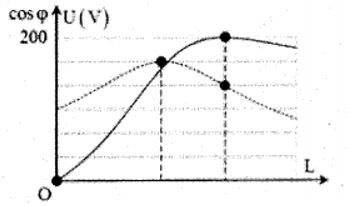
\includegraphics[scale=0.9]{../figs/VN12-PH-19-P-013-1-2.jpg}
		\end{center}
		\begin{mcq}(4)
			\item 240 V.
			\item 165 V.
			\item 220 V.
			\item 185 V.
		\end{mcq}
	}
	\loigiai{
		\textbf{Đáp án: B.}
		
		Khi xảy ra cực đại của điện áp hiệu dụng trên cuộn cảm thuần $$Z_L = \dfrac{R^2+Z^2_C}{Z_C}$$.
		
		Ta chuẩn hóa $R=1; Z_C = n \Rightarrow Z_L =\dfrac{1}{x} +x$.
		
		Hệ số công suất của mạch tương ứng $$\cos \varphi =\dfrac{R}{\sqrt{R^2 + (Z_L - Z_C)^2}} \Leftrightarrow \text{0,8} =\dfrac{1}{\sqrt {1+ \dfrac{1}{n^2}}} \Rightarrow n =\dfrac{4}{3}$$.
		
		Kết hợp với $$U_{L\text{max}} = U\sqrt {1+ \left (\dfrac{Z_C}{R}\right)^2} \Rightarrow U = \dfrac{U_{L_\text{max}}}{\sqrt {1+\left (\dfrac{Z_C}{R}\right)^2 }} =120\ \text{V}$$
		
		Suy ra $U_0 =120\sqrt 2 \approx 170\ \text{V}$.
		
		
	}
	
	%%%%%%%%%%%%%%CÂU4%%%%%%%%%%
	

	%%%%%%%%%%%%%%CÂU6%%%%%%%%%%
	\item \mkstar{4}
	
	\cauhoi{Đặt một điện áp xoay chiều có giá trị hiệu dụng và tần số không đổi vào hai đầu đoạn mạch điện AB gồm biến trở $R$, tụ điện $C$ và cuộn dây không thuần cảm có độ tự cảm $L$, điện trở thuần $r$, ghép nối tiếp với nhau như hình vẽ.
		\begin{center}
			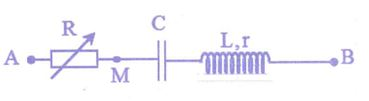
\includegraphics[scale=1]{../figs/VN12-PH-19-P-013-1-5.jpg}
		\end{center}
		Điều chỉnh R đến giá trị $60\ \Omega$ thì công suất tiêu thụ trên biến trở đạt cực đại, đồng thời tổng trở của đoạn mạch AB là số nguyên chia hết cho 45. Khi đó hệ số công suất của đoạn mạch MB có giá trị là
		
		\begin{mcq}(4)
			\item 0,375.
			\item 0,75.
			\item 0,125.
			\item 0,5.
		\end{mcq}
	}	
	\loigiai{
		\textbf{Đáp án: C.}
		
		Giá trị của biến trở để công suất tiêu thụ trên biến trở là cực đại:
		
		$$R=R_0 = \sqrt{r^2 +(Z_L-Z_C)^2} = 60\ \Omega$$
		
		+ Tổng trở của mạch khi đó
		
		$$Z= \sqrt{(R_0 +r)^2 +(Z_L-Z_C)^2} = \sqrt {R_0^2 + 2R_0r +r^2 +(Z_L-Z_C)^2}$$
		$$\Rightarrow Z^2 = 60^2 +2 \cdot 60 r + 60^2 = (n \cdot 45)^2 \Rightarrow r =\dfrac{135}{8}n^2 -60$$
		
		+ Hệ số công suất của đoạn mạch MB:
		
		$$\cos \varphi_\text{MB} = \dfrac{r}{\sqrt {r^2 + (Z_L-Z_C)^2 }} = \dfrac{\dfrac{135}{8}n^2 -60}{60}$$
		$$ 0<\cos \varphi_\text{MB} <1 \Leftrightarrow \text{1,89}<n<\text{2,7}$$
		
		$n=2$ suy ra $\cos \varphi_\text{MB} =\text{0,125}$. 
		
	}
	
	%%%%%%%%%%%%%%CÂU7%%%%%%%%%%
	
	
	%%%%%%%%%%%%%%CÂU8%%%%%%%%%%
	\item \mkstar{4}
	
	\cauhoi{Cho mạch điện như hình vẽ, cuộn dây thuần cảm. Điện áp hai đầu đoạn mạch có biểu thức $u= U\sqrt 2\cos 2\pi f t\ \text{V}$  với $U$ không đổi nhưng $f$ có thể thay đổi được. Ta có đồ thị biểu diễn sự phụ thuộc của công suất tiêu thụ trên mạch theo $R$ là đường liền nét khi $f=f_1$  và là đường đứt nét khi $f=f_2$. Giá trị của $P_\text{max}$  gần nhất với giá trị nào sau đây?
		\begin{center}
			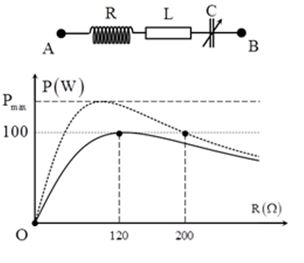
\includegraphics[scale=1.1]{../figs/VN12-PH-19-P-013-1-7.jpg}
		\end{center}
		\begin{mcq}(4)
			\item 280 W.
			\item 140 W.
			\item 130 W.
			\item 260 W.
		\end{mcq}
	}		
	\loigiai{
		\textbf{Đáp án: C.}
		
		+	$f=f_1$: Công suất cực đại của mạch khi $R_0 =120 = |Z_{L_1} - Z_{C_1}|.$
		
		Khi đó: $$P_{\text{max}_1} = \dfrac{U^2}{2|Z_{L_1} - Z_{C_1}|} \Rightarrow 100 =\dfrac{U^2}{2 \cdot 120} \Rightarrow U = 40\sqrt {15} \ \text{V}$$
		
		+ $f=f_2$: khi $R=200\ \Omega$ thì công suất tiêu thụ của mạch là 100 W.
		
		$$\Rightarrow 100 = \dfrac{(40\sqrt{15})^2}{200^2 + (Z_{L_2}-Z_{C_2})^2} \cdot 200 \Rightarrow |Z_{L_2}-Z_{C_2}| =40\sqrt 5.$$
		
		Khi đó: $P_\text{max} = P_{\text{max}_2} = \dfrac{U^2}{2|Z_{L_2}-Z_{C_2}|} =60\sqrt 5 \approx \text{134,16}\ \text{W}$.
		
		
	}
	
	%%%%%%%%%%%%%%CÂU9%%%%%%%%%%

\end{enumerate}
\loigiai{\textbf{Đáp án}
	\begin{center}
		\begin{tabular}{|m{2.8em}|m{2.8em}|m{2.8em}|m{2.8em}|m{2.8em}|m{2.8em}|m{2.8em}|m{2.8em}|m{2.8em}|m{2.8em}|}
			\hline
			1. A & 2. C & 3. C & 4. C & 5. D & 6. A  & 7. A  & 8. D & 9. C & 10. B\\
			\hline
			11. D & 12. B & 13. A & 14. A & 15. B & 16. D  & 17. B  & 18. B & 19. C & 20. C\\
			\hline
		\end{tabular}
\end{center}}
	\stopcontents[mychapters]

	
\setcounter{mychapter}{20}
	\mychapter{Điện từ trường - Sóng điện từ - Nguyên tắc thông tin liên lạc bằng sóng vô tuyến}
	\startcontents[mychapters]
	\printcontents[mychapters]{}{0}{\setcounter{tocdepth}{1}}
	\begin{enumerate}[label=\bfseries Câu \arabic*:]
	
	
	%%%%%%%%%%%%%%CÂU2%%%%%%%%%%
	\item \mkstar{1}
	
	\cauhoi{Một máy biến áp có số vòng dây của cuộn sơ cấp lớn hơn số vòng dây của cuộn thứ cấp. Máy biến áp này có tác dụng
		\begin{mcq}
			\item tăng cường độ dòng điện, giảm điện áp.
			\item giảm cường độ dòng điện, tăng điện áp.
			\item tăng cường độ dòng điện, tăng điện áp.
			\item giảm cường độ dòng điện, giảm điện áp.
		\end{mcq}
}	
		\loigiai{
			\textbf{Đáp án: A.}
			
			Máy biến áp có số vòng cuộn sơ cấp lớn hơn số vòng cuộn thứ cấp là máy hạ áp và có tác dụng làm tăng cường độ dòng điện.
			
			}	
	
	%%%%%%%%%%%%%%CÂU2%%%%%%%%%%
	\item \mkstar{1}
	
	\cauhoi{Hoạt động của máy biến áp dựa trên
		\begin{mcq}(2)
			\item hiên tượng tự cảm.
			\item hiên tượng cảm ứng điện từ.
			\item từ trường quay.
			\item tác dụng của lực từ.
		\end{mcq}
}	
		\loigiai{
			\textbf{Đáp án: B.}
			
			Hoạt động của máy biến áp dựa trên hiên tượng cảm ứng điện từ.
			
			}
	
	%%%%%%%%%%%%%%CÂU3%%%%%%%%%%
	\item \mkstar{1}
	
	\cauhoi{Nguyên nhân chủ yếu gây ra sự hao phí năng lượng trong máy biến thế là do
		\begin{mcq}
			\item hao phí năng lượng dưới dạng nhiệt năng tỏa ra ở các cuộn sơ cấp và thứ cấp của máy biến thế.
			\item lõi sắt có từ trở và gây dòng Fu-cô.
			\item có sự thất thoát năng lượng dưới dạng bức xạ điện từ.
			\item Cả 3 ý kiến trên.
		\end{mcq}
}	
		\loigiai{
			\textbf{Đáp án: D.}
			
			Nguyên nhân chủ yếu gây ra sự hao phí năng lượng trong máy biến thế là do
			\begin{itemize}
				\item hao phí năng lượng dưới dạng nhiệt năng tỏa ra ở các cuộn sơ cấp và thứ cấp của máy biến thế.
				\item lõi sắt có từ trở và gây dòng Fu-cô.
				\item có sự thất thoát năng lượng dưới dạng bức xạ điện từ.
			\end{itemize}
			
			}
	
	%%%%%%%%%%%%%%CÂU4%%%%%%%%%%
	\item \mkstar{1}
	
	\cauhoi{Vai trò của máy biến thế trong truyền tải điện năng là
		\begin{mcq}
			\item giảm điện trở của dây dẫn trên đường truyền tải để giảm hao phí trên đường truyền tải.
			\item tăng hiệu điện thế truyền tải để giảm hao phí trên đường truyền tải.
			\item giảm hiệu điện thế truyền tải để giảm hao phí trên đường truyền tải.
			\item giảm sự thất thoát năng lượng dưới dạng bức xạ sóng điện từ.
		\end{mcq}
}	
		\loigiai{
			\textbf{Đáp án: B.}
			
			Vai trò của máy biến thế trong truyền tải điện năng là tăng hiệu điện thế truyền tải để giảm hao phí trên đường truyền tải.
			
			}	
	
	%%%%%%%%%%%%%%CÂU5%%%%%%%%%%
	\item \mkstar{2}
	
	\cauhoi{Chọn câu đúng.
		\begin{mcq}
			\item Khi mạch thứ cấp hở dòng điện ở cuộn sơ cấp luôn bằng 0. 
			\item Dòng điện trong cuộn sơ cấp là dòng điện cảm ứng.
			\item Cuộn sơ cấp là máy thu điện.
			\item Cường độ dòng điện trong mạch sơ cấp khác nhau trong hai trường hợp mạch thứ cấp kín và hở.
		\end{mcq}
}	
		\loigiai{
			\textbf{Đáp án: D.}
			
		Cường độ dòng điện trong mạch sơ cấp khác nhau trong hai trường hợp mạch thứ cấp kín và hở.	
			
			}	
	
	%%%%%%%%%%%%%%CÂU6%%%%%%%%%%
	\item \mkstar{2}
	
	\cauhoi{Máy biến thế có thể dùng để biến đổi hiệu điện thế của nguồn điện nào sau đây?
		\begin{mcq}(2)
			\item Pin.
			\item Ac-quy.
			\item Nguồn điện xoay chiều AC.
			\item Nguồn điện một chiều DC.
		\end{mcq}
}	
		\loigiai{
			\textbf{Đáp án: C.}
			
			Máy biến thế có thể dùng để biến đổi hiệu điện thế của nguồn điện xoay chiều AC.
			
			}	
	
	%%%%%%%%%%%%%%CÂU7%%%%%%%%%%
	\item \mkstar{2}
	
	\cauhoi{Người ta dùng lõi thép kĩ thuật điện trong máy biến áp, mục đích chính là để
		\begin{mcq}
			\item làm mạch dẫn dòng điện từ cuộn sơ cấp sang cuộn thứ cấp.
			\item làm mạch từ và tăng cường từ thông qua các cuộn dây.
			\item làm giảm hao phí do tỏa nhiệt bởi dòng điện Fu-cô.
			\item làm khung lắp cuộn sơ cấp và cuộn thứ cấp trên nó.
		\end{mcq}
	}
		\loigiai{
			\textbf{Đáp án: B.}
			
			Người ta dùng lõi thép kĩ thuật điện trong máy biến áp, mục đích chính là để làm mạch từ và tăng cường từ thông qua các cuộn dây.
			
			}
	
	%%%%%%%%%%%%%%CÂU8%%%%%%%%%%
	\item \mkstar{2}
	
	\cauhoi{Biện pháp nào sau đây \textbf{không} góp phần tăng hiệu suất của máy biến áp?
		\begin{mcq}
			\item Đặt các lá sắt của lõi sắt song song với mặt phẳng chứa các đường sức từ.
			\item Dùng lõi sắt gồm nhiều lá sắt mỏng ghép cách điện với nhau.
			\item Dùng dây có điện trở suất nhỏ là dây quấn biến áp.
			\item Dùng lõi sắt có điện trở suất nhỏ.
		\end{mcq}
}	
		\loigiai{
			\textbf{Đáp án: D.}
			
			Dùng lõi sắt có điện trở suất nhỏ thì điện trở nhỏ, giảm công suất nên không góp phần tăng hiệu suất của máy biến áp.
			
			}	
	
	%%%%%%%%%%%%%%CÂU9%%%%%%%%%%
	\item \mkstar{2}
	
	\cauhoi{Người ta cần truyền một công suất điện 200 kW từ nguồn điện có điện áp 5000 V trên đường dây có điện trở tổng cộng $20\ \Omega$ và hệ số công suất bằng 1. Độ giảm thế trên đường dây tải điện là
		\begin{mcq}(4)
			\item 40 V.
			\item 400 V.
			\item 80 V.
			\item 800 V.
		\end{mcq}
}	
		\loigiai{
			\textbf{Đáp án: D.}
			
			\begin{itemize}
				\item Áp dụng công thức công suất hao phí do tỏa nhiệt trên đường dây
				
				\begin{equation*}
					\Delta P = I^2R =R\dfrac{P^2}{(U \cos \varphi)^2}.
				\end{equation*}
				\item Suy ra độ giảm thế trên đường dây truyền tải
				\begin{equation*}
					\Delta U = IR = \dfrac{P}{U \cos \varphi}R = 800\ \text{V}.
				\end{equation*}
			\end{itemize}
			
			}
	
	%%%%%%%%%%%%%%CÂU10%%%%%%%%%%
	\item \mkstar{2}
	
	\cauhoi{Một máy tăng áp có tỉ số vòng dây giữa hai cuộn dây là 2. Đặt vào hai đầu cuộn sơ cấp một điện áp xoay chiều có tần số $\SI{50}{Hz}$. Tần số dòng điện hai đầu cuộn thứ cấp bằng
		\begin{mcq}(4)
			\item $\SI{50}{Hz}$.
			\item $\SI{25}{Hz}$.
			\item $\SI{100}{Hz}$.
			\item $50\sqrt{2}\ \SI{}{Hz}$.
		\end{mcq}
	}
		\loigiai{
			\textbf{Đáp án: A.}
			
			Máy biến áp không làm thay đổi tần số của dòng điện qua nó.
			
			}
	
	%%%%%%%%%%%%%%CÂU11%%%%%%%%%%
	\item \mkstar{2}
	
	\cauhoi{Trạm phát điện truyền đi công suất $\SI{550}{kW}$, điện áp nơi phát bằng $\SI{10}{kV}$. Muốn độ giảm điện áp trên dây tải không vượt quá $10\%$ điện áp nơi phát thì điện trở của dây tải điện không được vượt quá giá trị
		\begin{mcq}(4)
			\item $\SI{18}{\ohm}$.
			\item $\SI{11}{\ohm}$.
			\item $\SI{55}{\ohm}$.
			\item $\SI{5,5}{\ohm}$.
		\end{mcq}
}	
		\loigiai{
			\textbf{Đáp án: A.}
			
			Công suất hao phí là
			$$\Delta=R\left(\dfrac{P}{U}\right)^2\leq \dfrac{10}{100}P\Rightarrow R\leq \dfrac{0,1U^2}{P}=\SI{18}{\ohm}.$$
			
			}
	
	%%%%%%%%%%%%%%CÂU12%%%%%%%%%%
	\item \mkstar{2}
	
	\cauhoi{Một máy biến áp lý tưởng có tỉ số giữa số vòng dây của cuộn sơ cấp và số vòng dây của cuộn thứ cấp bằng 10. Mắc một bóng đèn sợi đốt loại $\SI{24}{V}$ – $\SI{24}{W}$ vào hai đầu cuộn thứ cấp thì đèn sáng bình thường. Cường độ dòng điện hiệu dụng trong cuộn sơ cấp bằng
		\begin{mcq}(4)
			\item $\SI{0,2}{A}$.
			\item $\SI{0,5}{A}$.
			\item $\SI{0,1}{A}$.
			\item $\SI{2}{A}$.
		\end{mcq}
}	
		\loigiai{
			\textbf{Đáp án: C.}
			
			Dòng điện qua đèn để đèn sáng bình thường
			$$I_\textrm{đ}=I_2=\dfrac{P}{U}=\SI{1}{A}.$$
			
			Dòng điện ở cuộn sơ cấp là
			$$I_1=\dfrac{I_2}{n}=\SI{0,1}{A}.$$
			}
	
	%%%%%%%%%%%%%%CÂU13%%%%%%%%%%
	\item \mkstar{2}
	
	\cauhoi{Đặt vào hai đầu cuộn sơ cấp của một máy biến áp lí tưởng (bỏ qua hao phí) một điện áp xoay chiều có giá trị hiệu dụng không đổi thì điện áp hiệu dụng giữa hai đầu cuộn thứ cấp để hở là $100\ V$. Ở cuộn thứ cấp, nếu giảm bớt n vòng dây thì điện áp hiệu dụng giữa hai đầu để hở của nó là $U$, nếu tăng thêm $n$ vòng dây thì điện áp đó là $2U$. Nếu tăng thêm $3n$ vòng dây ở cuộn thứ cấp thì điện áp hiệu dụng giữa hai đầu để hở của cuộn này bằng
		\begin{mcq}(4)
			\item $\SI{200}{V}$.
			\item $\SI{220}{V}$.
			\item $\SI{110}{V}$.
			\item $\SI{100}{V}$.
		\end{mcq}
}	
		\loigiai{
			\textbf{Đáp án: A.}
			
			Ta có: $$\left\{\begin{array}{l}\dfrac{\mathrm{N}_{2}}{\mathrm{N}_{1}}=\dfrac{100}{\mathrm{U}_{1}} \\ \dfrac{\mathrm{N}_{2}-\mathrm{n}}{\mathrm{N}_{1}}=\dfrac{\mathrm{U}}{\mathrm{U}_{1}} \Rightarrow \mathrm{N}_{2}=3 \mathrm{n} \\ \dfrac{\mathrm{N}_{2}+\mathrm{n}}{\mathrm{N}_{1}}=\dfrac{2 \mathrm{U}}{\mathrm{U}_{1}}.\end{array}\right.$$
			
			Vậy khi số vòng tăng 3n vòng thì tỉ số $$\dfrac{N_2+3n}{N_1}=\dfrac{2N_2}{N_1}=\dfrac{U_2}{U_1}\Rightarrow\dfrac{200}{U_1}=\dfrac{U_2}{U_1}\Rightarrow \SI{200}{V}.$$
			
			}
	
	%%%%%%%%%%%%%%CÂU14%%%%%%%%%%
	\item \mkstar{2}
	
	\cauhoi{Cho một máy biến áp có hiệu suất $80\%$. Cuộn sơ cấp có 100 vòng, cuộn thứ cấp có 200 vòng. Mạch sơ cấp lý tưởng, đặt vào hai đầu cuộn sơ cấp điện áp xoay chiều có giá trị hiệu dụng 100 V và tần số 50 Hz. Hai đầu cuộn thứ cấp nối với một cuộn dây có điện trở $50\ \Omega$, độ tự cảm $\dfrac{\text{0,5}}{\pi}\ \text{H}$. Cường độ dòng điện hiệu dụng mạch sơ cấp nhận giá trị
		\begin{mcq}(4)
			\item 5 A.
			\item 10 A.
			\item 2 A.
			\item 2,5 A.
		\end{mcq}
}	
		\loigiai{
			\textbf{Đáp án: A.}
			
			\begin{itemize}
				\item Áp dụng công thức suy ra điện áp của cuộn thứ cấp
				\begin{equation*}
					\dfrac{U_2}{U_1}=\dfrac{N_2}{N_1} \Rightarrow U_2= \dfrac{N_2}{N_1}U_1 = 200\ \text{V}.
				\end{equation*}
				\item Cường độ dòng điện qua cuộn thứ cấp
				\begin{equation*}
					I_2 = \dfrac{U_2}{\sqrt{R^2+Z_L^2}}= 2\sqrt 2\ \text{A}.
				\end{equation*}
				\item Hiệu suất của máy biến áp 
				\begin{equation*}
					H=\dfrac{I^2_2R}{U_1I_1}.
				\end{equation*}
				\item Suy ra cường độ dòng điện qua cuộn sơ cấp 
				\begin{equation*}
					I_1= \dfrac{I^2_2R}{HU_1}=5\ \text{A}.
				\end{equation*}
			\end{itemize}
			
			}
	
	%%%%%%%%%%%%%%CÂU15%%%%%%%%%%
	\item \mkstar{3}
	
	\cauhoi{Một đường dây có điện trở tổng cộng $4\ \Omega$ dẫn một dòng điện xoay chiều một pha từ nơi sản xuất đến nơi tiêu dùng. Điện áp hiêu dụng ở nguồn điện lúc phát ra là 10 kV, công suất điện là 400 kW. Hệ số công suất của mạch điện là $\cos \varphi = \text {0,8}$. Có bao nhiêu phần trăm công suất bị hao phí trên đường dây do tỏa nhiệt?
		
		\begin{mcq}(4)
			\item 1,6$\%$.        
			\item 2,5$\%$.
			\item 6,4$\%$.       
			\item 10$\%$.
		\end{mcq}
}	
		\loigiai{
			\textbf{Đáp án: B.}
			
			\begin{itemize}
				\item  Công suất hao phí trên đường dây tải điện
				\begin{equation*}
					\Delta P= I^2R = \left(\dfrac{P}{U\cos \varphi}\right)^2R.
				\end{equation*}
				\item Hiệu suất truyền tải điện 
				\begin{equation*}
					H = \dfrac{P-\Delta P}{P}=1-\dfrac{\Delta P}{P}.
				\end{equation*}
				\item Phần trăm công suất bị hao phí
				\begin{equation*}
					h= \dfrac{\Delta P}{P}= \dfrac{PR}{U^2 \cos^2 \varphi} = \text{0,025}= \text{2,5}\ \%.
				\end{equation*}
			\end{itemize}
			
			
			}
	
	%%%%%%%%%%%%%%CÂU16%%%%%%%%%%
	\item \mkstar{3}
	
	\cauhoi{Ở trạm phát điện xoay chiều một pha có điện áp hiệu dụng 110 kV, truyền đi công suất điện 1000 kW trên đường dây dẫn có điện trở $20\ \Omega$. Hệ số công suất của đoạn mạch $\cos \varphi =\text{0,9}$. Điện năng hao phí trên đường dây trong 30 ngày là
		
		\begin{mcq}(4)
			\item 5289 kWh.
			\item 61,2 kWh.
			\item 145,5 kWh.
			\item 1469 kWh.
		\end{mcq}
	}
		\loigiai{
			\textbf{Đáp án: D.}
			
			\begin{itemize}
				\item Công suất hao phí trên đường dây tải điện
				\begin{equation*}
					\Delta P = \left(\dfrac{P}{U\cos \varphi}\right)^2 \cdot R = \text{2040,6}\ \text{W}.
				\end{equation*}
				\item Thời gian 30 ngày $t=30 \cdot 24 =720 \ \text{giờ}$.
				\item Điện năng hao phí trên đường dây trong 30 ngày
				\begin{equation*}
					A= \Delta P \cdot t = 1469232\ \text{W} \approx  1469\ \text{kWh}.
				\end{equation*}
			\end{itemize}
			
			}
	
	%%%%%%%%%%%%%%CÂU17%%%%%%%%%%
	\item \mkstar{3}
	
	\cauhoi{Người ta truyền tải điện xoay chiều một pha từ một trạm phát điện đến nơi tiêu thụ bằng dây dẫn có tổng chiều dài 20 km. Dây dẫn làm bằng kim loại có điện trở suất $\text{2,5}\cdot 10^{-8}\ \Omega m$, tiết diện $\text{0,4}\ \text{cm}^2$, hệ số công suất của mạch điện là 1. Điện áp hiệu dụng và công suất truyền đi ở trạm phát điện là $10\ \text{kV}$ và 500 kW. Hiệu suất truyền tải điện là
			\begin{mcq}(4)
				\item 93,75$\%$.        
				\item 96,14$\%$.
				\item 97,41$\%$.        
				\item 96,88$\%$.
			\end{mcq}
	}	
			\loigiai{
				\textbf{Đáp án: A.}
				
				\begin{itemize}
					\item Điện trở đường dây tải điện
					\begin{equation*}
						R = \rho \dfrac{l}{S}=\text{12,5}\ \Omega.
					\end{equation*}
					\item  Công suất hao phí trên đường dây tải điện
					\begin{equation*}
						\Delta P= I^2R = \left(\dfrac{P}{U\cos \varphi}\right)^2R= \text{31250}\ \text{W}.
					\end{equation*}
					\item Hiệu suất truyền tải điện 
					\begin{equation*}
						H = \dfrac{P-\Delta P}{P}=1-\dfrac{\Delta P}{P}= \text{93,75}\% .
					\end{equation*}
				\end{itemize}
				
				}
		
		%%%%%%%%%%%%%%CÂU18%%%%%%%%%%
		\item \mkstar{3}
		
		\cauhoi{Một máy phát điện xoay chiều có công suất 1000 kW. Dòng điện nó phát ra sau khi tăng thế được truyền đi xa bằng một dây dẫn có tổng chiều dài 200 km có đường kính 0,39 cm và bằng hợp kim có điện trở suất bằng $\text {1,8} \cdot 10^{-8}\ \Omega \text{m}$. Biết hệ số công suất đường dây bằng 1. Tính công suất hao phí trên đường dây nếu điện áp đưa lên là 50 kV.
			\begin{mcq}(4)
				\item 0,16 MW.
				\item 0,03 MW.
				\item 0,2 MW.
				\item 0,12 MW.
			\end{mcq}
	}	
			\loigiai{
				\textbf{Đáp án: A.}
				
				\begin{itemize}
					\item Diện tích hình tròn
					\begin{equation*}
						S=\pi r^2=\pi \dfrac{d^2}{4}=\text{1,19}\cdot 10^{-5}\ \text{cm}^2.
					\end{equation*}
					\item Điện trở đường dây
					\begin{equation*}
						R=\rho \dfrac{l}{S}= 301\ \Omega.
					\end{equation*}
					\item Công suất hao phí trên đường dây
					\begin{equation*}
						\Delta P =R\dfrac{P^2}{(U \cos \varphi)^2} \approx \text {0,12} \cdot 10^{6}\ \text{W}
					\end{equation*}
				\end{itemize}	
				
				}
		
		%%%%%%%%%%%%%%CÂU19%%%%%%%%%%
		
			\item \mkstar{3}
			
			\cauhoi{Điện năng được truyền tải từ nhà máy thủy điện đến khu dân cư có công suất tiêu thụ không đổi. Khi truyền đi với điện áp là $U$  thì độ giảm điện áp trên đường dây tải điện bằng $\dfrac{U}{10}$. Coi cường độ dòng điện trong mạch luôn cùng pha với điện áp đặt lên đường dây, điện trở của đường dây luôn không đổi. Để hao phí trên đường dây giảm 144 lần thì cần tăng điện áp truyền đi lên gần nhất giá trị nào sau đây?
				\begin{mcq}(4)
					\item 8 lần.
					\item 9 lần.
					\item 10 lần.
					\item 11 lần.
				\end{mcq}
	}		
				\loigiai{
				\textbf{Đáp án: D.}
					
					$P_\text{tt} =U_\text{tt} I$ không đổi nên $I$ và $U_\text{tt}$ tỉ lệ nghịch với nhau.
					
					$\Delta P = I^2R$ suy ra $\Delta P $ giảm 144 lần thì $I$ giảm 12 lần (lưu ý, ta không dùng $\Delta P =\dfrac{PR}{U^2}$ để biện luận vì bài toán không ràng buộc điều kiện $P$  không đổi)		
					Ta lập bảng số liệu cho hai trường hợp:
					
					\begin{center}
						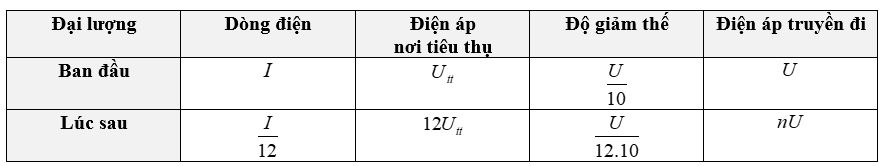
\includegraphics[scale=0.8]{../figs/VN12-PH-21-P-015-1-1.jpg}
					\end{center}
					
					Ta có: 
					
					$12U_\text{tt} =nU - \dfrac{U}{12 \cdot 10} \Rightarrow 12 \left(U-\dfrac{U}{10}\right) = nU -	\dfrac{U}{12 \cdot 10} \Rightarrow n = \text{10,8}$.
					
					}
			
			%%%%%%%%%%%%%%CÂU2%%%%%%%%%%
			\item \mkstar{3}
			
			\cauhoi{Điện năng được truyền từ nơi phát đến một khu dân cư bằng đường dây một pha với hiệu suất truyền tải là $80\%$. Coi hao phí điện năng chỉ do tỏa nhiệt trên đường dây và không vượt quá $20\%$. Nếu công suất sử dụng điện của khu dân cư này tăng $50\%$ và giữ nguyên điện áp ở nơi phát thì hiệu suất truyền tải điện năng trên chính đường dây đó gần nhất giá trị nào sao đây?
				\begin{mcq}(4)
					\item $80\%$.
					\item $70\%$.
					\item $90\%$.
					\item $85\%$.
				\end{mcq}
		}	
				\loigiai{
					\textbf{Đáp án: B.}
					
					Nhận thấy rằng, trong trường hợp thứ hai của bài toán truyền tải, công suất nơi tiêu thụ tăng. Do đó công suất truyền tải lúc sau cũng phải tăng theo.
					
					Vì điện áp ở nơi truyền tải được giữ không đổi, nếu tăng $nP$  thì dòng điện lúc sau là $nI$. Ta lập bảng tỉ lệ
					\begin{center}
						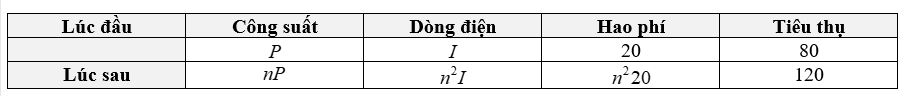
\includegraphics[scale=0.8]{../figs/VN12-PH-21-P-015-1-2.jpg}
					\end{center}
					Ta có 
					
					$100n =20n^2 + 120$ suy ra $n =3$ hoặc $n=2$.
					
					$n=2$ thì $\dfrac{\Delta P}{P} = \dfrac{20n}{100} = \text{0,4} \Rightarrow H = \text{0,6}\ \text{nhận}$.
					
					$n=3$ thì $\dfrac{\Delta P}{P} = \dfrac{20n}{100} = \text{0,6} > \text{0,5} \Rightarrow H = \text{0,4}\ \text{loại}$.
					
					}
			
			%%%%%%%%%%%%%%CÂU3%%%%%%%%%%
			\item \mkstar{3}
			
			\cauhoi{Điện năng được truyền từ trạm phát điện đến nơi tiêu thụ bằng đường dây tải điện một pha. Ban đầu hiệu suất truyền tải là $60\%$. Cho công suất truyền đi không đổi và hệ số công suất ở nơi tiêu thụ (cuối đường dây tải điện) luôn bằng 0,8. Để giảm hao phí trên đường dây 4 lần thì cần phải tăng điện áp hiệu dụng ở trạm phát điện lên $n$  lần. Giá trị của $n$  là
				\begin{mcq}(4)
					\item 2,0.
					\item 2,1.
					\item 2,3.
					\item 2,2.
				\end{mcq}
		}	
				\loigiai{
					\textbf{Đáp án: D.}
					
					Ta biễu diễn mối liên hệ giữa các điện áp trong quá trình truyền tải
					\begin{center}
						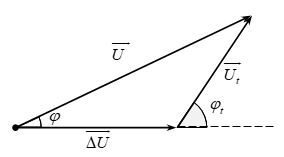
\includegraphics[scale=0.8]{../figs/VN12-PH-21-P-015-1-3.jpg}
					\end{center}
					$$U \cos \varphi =U_\text{t} \cos \varphi_\text{t}$$.
					$$P_\text{tt} = HP \Rightarrow U_\text{t} I \cos \varphi_\text{t} = H(UI \cos \varphi) \Rightarrow U\cos \varphi = \dfrac{U_\text{t} \cos \varphi_\text{t}}{H}$$
					
					Từ hai phương trình trên, ta có $\tan \varphi = H \tan \varphi_\text{t}$. 
					
					Tiến hành lập bảng tỉ lệ
					\begin{center}
						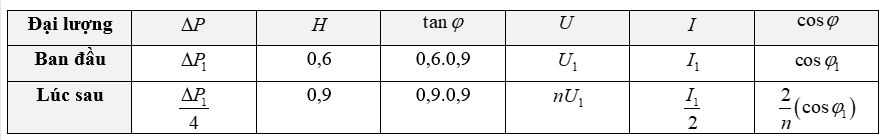
\includegraphics[scale=0.8]{../figs/VN12-PH-21-P-015-1-4.jpg}
					\end{center}
					Ta có
					
					$$\left (\dfrac{\cos \varphi_2}{\cos \varphi_1}\right)^2 = \dfrac{4}{n^2} = \dfrac {1+\tan ^2 \varphi_1}{1+ \tan^2 \varphi_2} \Rightarrow n \approx \text{2,2}$$
					
					}
			
			%%%%%%%%%%%%%%CÂU4%%%%%%%%%%
			\item \mkstar{2}
			
			\cauhoi{Một trạm phát điện truyền đi công suất 1000 kW bằng dây dẫn có điện trở tổng cộng $8\ \Omega$  điện áp ở hai cực của máy là 1000 V. Hai cực của máy được nối với hai đầu cuộn sơ cấp của máy tăng áp lý tưởng mà số vòng dây của cuộn thứ cấp gấp 10 lần số vòng dây cuộn sơ cấp. Biết hệ số công suất của đường dây bằng 1. Hiệu suất quá trình truyền tải:
				\begin{mcq}(4)
					\item $92\%$..
					\item $95\%$..
					\item $80\%$..
					\item $87\%$..
				\end{mcq}
		}	
				\loigiai{
					\textbf{Đáp án: A.}
					
					Điện áp phát ra ở hai đầu cuộn thứ cấp: 
					
					$$\dfrac{U_1}{U_2} =\dfrac{N_1}{N_2} \Rightarrow U_2 =U_1 \dfrac{N_2}{N_1} = 10^4\ \text{V}$$
					
					Công suất hao phí: $$\Delta P = \dfrac{P^2R}{U^2_2 \cos^2 \varphi}$$
					
					Hiệu suất quá trình truyền tải: $$H = 1- \dfrac{\Delta P}{P} = \text{0,92} = 92\%$$
					
				}
			
			%%%%%%%%%%%%%%CÂU5%%%%%%%%%%
			\item \mkstar{3}
			
			\cauhoi{Khi đặt một điện áp xoay chiều có giá trị hiệu dụng không đổi vào hai đầu cuộn sơ cấp của một máy biến áp thì điện áp hiệu dụng ở hai đầu thứ cấp để hở là 20 V. Khi tăng số vòng dây cuộn thứ cấp thêm 60 vòng thì điện áp hiệu dụng hai đầu thứ cấp là 25 V. Khi giảm số vòng dây thứ cấp đi 90 vòng thì điện áp hiệu dụng hai đầu thứ cấp để hở là
				\begin{mcq}(4)
					\item 17,5 V.
					\item 15 V.
					\item 10 V.
					\item 12,5 V.
				\end{mcq}
		}	
				\loigiai{
					\textbf{Đáp án: D.}
					
					Ta có:$$\dfrac{U_1}{20} =\dfrac{N_1}{N_2} (1); \dfrac{U_1}{25} = \dfrac{N_1}{N_2+60} (2); \dfrac{U_1}{U_3} = \dfrac{N_1}{N_2 - 90} (3)$$
					Chia vế với vế của (1) cho (2), được: $$\dfrac{25}{20} = \dfrac{N_2 +60}{N_2} \Rightarrow N_2 = 240\ \text{vòng}$$
					Chia vế với vế của (1) cho (3), được: $$\dfrac{U_3}{20}=\dfrac{N_2 - 90}{N_2} \Rightarrow U_3 =\text{12,5}\ \text{V}$$
					
					}
			
			%%%%%%%%%%%%%%CÂU6%%%%%%%%%%
			\item \mkstar{3}
			
			\cauhoi{Điện năng từ một trạm phát điện được đưa đến một khu tái định cư bằng dây truyền tải một pha. Cho biết, nếu điện áp tạo đầu truyền đi tăng từ $U$ lên $2U$ thì số hộ dân được trạm cung cấp đủ điện năng từ 120 lên 144. Cho rằng chỉ tính đến hao phí trên đường dây, công suất tiêu thụ điện của các hộ dân đều như nhau, công suất của trạm phát không đổi và hệ số công suất trong các trường hợp đều bằng nhau. Nếu điện áp truyền đi là $4U$ thì trạm phát này cung cấp đầy đủ điện năng cho
				\begin{mcq}(4)
					\item 168 hộ dân.
					\item 504 hộ dân.
					\item 192 hộ dân.
					\item 150 hộ dân.
				\end{mcq}
	}		
				\loigiai{
				\textbf{Đáp án: D.}
					
					Ta xét các trường hợp:
					
					+ Khi $U$ tăng lên 2 $\Rightarrow$ công suất hao phí giảm 4: $\dfrac{\Delta P}{4}$.  
					
					$\Rightarrow$ Công suất điện cấp cho hộ dân tăng lên $\dfrac{3\Delta P}{4}$  tương ứng với $144-120 =24$ hộ dân.
					
					+ Khi $U$ tăng lên 4 $\Rightarrow$ công suất hao phí giảm 16: $\dfrac{\Delta P}{16}$.
					
					$\Rightarrow$ Công suất điện cấp cho hộ dân tăng lên $\dfrac{15\Delta P}{16}$  tương ứng với $\dfrac{\dfrac{15 \Delta P}{16} \cdot 24}{\dfrac{3\Delta P}{4}}=30$ hộ dân.
					
					$\Rightarrow$ Điện áp $4U$ sẽ cấp đủ cho $120 + 30 =150$ hộ dân. 
					
					}
			
			%%%%%%%%%%%%%%CÂU7%%%%%%%%%%
			\item \mkstar{3}
			
			\cauhoi{Điện năng được truyền từ một nhà máy phát điện có công suất không đổi đến một khu công nghiệp bằng đường dây tải điện một pha. Nếu điện áp hiệu dụng truyền đi là $U$ và ở khu công nghiệp lắp một máy hạ áp lý tưởng có hệ số biến áp là 54 thì đáp ứng được $\dfrac{12}{13}$ nhu cầu sử dụng điện của công nghiệp. Coi cường độ dòng điện và điện áp luôn cùng pha. Muốn cung cấp đủ điện năng cho khu công nghiệp với điện áp truyền đi là $2U$ thì ở khu công nghiệp cần dùng máy hạ áp lý tưởng hệ số biến áp là
				\begin{mcq}(4)
					\item 114.
					\item 111.
					\item 117.
					\item 108.
				\end{mcq}
		}	
				\loigiai{
					\textbf{Đáp án: C.}
					
					+ Gọi $U_0$ là điện áo cuộn thứ cấp. Khi $k=54$ suy ra điện áp cuộn sơ cấp là $54U_0$.
					
					Khi $k=n$ thì điện áp cuộn sơ cấp là $nU_0$.
					
					+ Khi điện áp hiệu dụng là $U$ thì hao phí là $\Delta P \Rightarrow P - \Delta P =12 (1)$.
					+ Khi điện áp hiệu dụng là $2U$ thì hao phí là $\dfrac{\Delta P}{4} \Rightarrow P- \dfrac{\Delta P}{4} =13(2)$.
					
					+ Giải (1) và (2) ta được: $P =\dfrac{40}{3}\ \text{W}$ và $\Delta P =\dfrac{4}{3}$.
					
					Suy ra:
					
					$$H_1 =\dfrac{P-\Delta P}{P} =\text{0,9} = \dfrac{54U_0}{U} \Rightarrow \dfrac{U_0}{U} = \dfrac{1}{60}$$
					$$H_2 = \dfrac{P-\dfrac{\Delta P}{4}}{P} = \dfrac{39}{40} =\dfrac{nU_0}{2U} \Rightarrow n = 117$$	
					
					
					}
			
			%%%%%%%%%%%%%%CÂU8%%%%%%%%%%
			\item \mkstar{3}
			
		\cauhoi{Một máy hạ thế có tỉ số giữa số vòng dây cuộn sơ cấp và số vòng cuộn thứ cấp là $k$ $(k>1)$. Nhưng do không ghi kí hiệu trên máy nên không biết được số vòng trên các cuộn sơ cấp và thứ cấp. Một người đã dùng máy biến thế trên lần lượt đấu hai đầu mỗi cuộn dây của máy vào mạng điện xoay chiều có điện áp hiệu dụng không đổi $U$ và dùng vôn kế đo điện áp hiệu dụng ở hai đầu cuộn dây còn lại. Kết quả lần đo thứ nhất thu được là 250 V, lần đo thứ 2 là 10 V. Tỉ số $k$ bằng
				\begin{mcq}(4)
					\item 8.
					\item 2.
					\item 5.
					\item 16.
				\end{mcq}
		}	
				\loigiai{
					\textbf{Đáp án: D.}
					
					Do đây là máy hạ thế nên số vòng cuộn sơ cấp $N_1$  nhiều hơn số vòng cuộn thứ cấp $N_2$
					
					Lần đo thứ nhất: $$k = \dfrac{N_1}{N_2} = \dfrac{250}{U} (1)$$
					
					Lần đo thứ hai: $$k =\dfrac{N_1}{N_2} =\dfrac{U}{10} (2)$$
					
					Từ (1) và (2) ta có $$\dfrac{250}{U} =\dfrac{U}{10} \Rightarrow U =50\ \text{V} \Rightarrow k =5$$
					
					}
			
			%%%%%%%%%%%%%%CÂU9%%%%%%%%%%
			\item \mkstar{3}
			
			\cauhoi{Cho một máy biến áp lí tưởng, cuộn sơ cấp có $N_1$ vòng dầy, cuộn thứ cấp có $N_2$ vòng dây. Nếu giữ nguyên điện áp hiệu dụng hai đầu cuộn sơ cấp, rồi quấn thêm vào cuộn sơ cấp 25 vòng thì điện áp hiệu dụng ở hai đầu cuộn thứ cấp giảm đi $\dfrac{100}{13}\%$ . Còn nếu quấn thêm vào cuộn thứ cấp 25 vòng và muốn điện áp hiệu dụng hai đầu cuộn này không đổi thì phải giảm điện áp hiệu dụng hai đầu cuộn sơ cấp $\dfrac{100}{13}\%$ . Hệ số máy biến áp $k =\dfrac{N_1}{N_2}$  là
				\begin{mcq}(4)
					\item 6,5.
					\item 13.
					\item 6.
					\item 12.
				\end{mcq}
		}	
				\loigiai{
					\textbf{Đáp án: C.}
					
					Hệ số máy biến áp: $k= \dfrac{N_1}{N_2} =\dfrac{U_1}{U_2}$.
					
					+	Lần đo thứ nhất:
					
					Hiệu điện thế và số vòng dây trên cuộn sơ cấp: $U_1; N_1 + 25$.
					
					Hiệu điện thế và số vòng dây trên cuộn thứ cấp: $U'_2 =U_2 -\dfrac{1}{13}U_2; N_2$.
					
					Ta có: $$\dfrac{N_1 +25}{N_2} =\dfrac{U_1}{U_2 \left(1-\dfrac{1}{13}\right)} \Leftrightarrow k+\dfrac{25}{N_2} = \dfrac{13}{12} k$$
					
					$$N_2 =\dfrac{300}{k}; N_1 =kN_2=300.(*)$$ 
					
					+	Lần đo thứ hai:
					
					Hiệu điện thế và số vòng dây trên cuộn sơ cấp: $U'_1 = U_1 -\dfrac{1}{3}U_1; N_1$.
					
					Hiệu điện thế và số vòng dây trên cuộn thứ cấp: $U_2; N_2 + 25$.
					
					Ta có: $$\dfrac{N_1}{N_2 +25} =\dfrac{U_1\left(1-\dfrac{1}{13}\right)}{U_2 } \Leftrightarrow \dfrac{N_1}{N_2+25} = \dfrac{2}{3} k$$
					
					Thay (*) vào suy ra $k =6$.
					
					}
			
			%%%%%%%%%%%%%%CÂU10%%%%%%%%%%
			\item \mkstar{3}
			
		\cauhoi{Trong giờ học thực hành, học sinh muốn tạo một máy biến thế với số vòng dây ở cuộn sơ cấp gấp 4 lần cuộn thứ cấp. Do xảy ra sự cố nên cuộn thứ cáp bị thiếu một số vòng dây. Để xác định số vòng dây bị thiếu, học sinh này dùng vôn kế lý tưởng và đo được tỉ số điện áp hiệu dụng ở cuộn thứ cấp và cuộn sơ cấp là $\dfrac{43}{200}$ . Sau đó học sinh quấn thêm vào cuộn thứ cấp 48 vòng nữa thì tỷ số điện áp hiệu dụng nói trên là $\dfrac{9}{40}$ . Bỏ qua mọi hao phí của máy biến áp. Để được máy biến áp có số vòng dây đúng như dự định thì học sinh đó phải cuốn tiếp bao nhiêu vòng?
				\begin{mcq}(4)
					\item 168 vòng.
					\item 120 vòng.
					\item 60 vòng.
					\item 50 vòng.
				\end{mcq}
		}	
				\loigiai{
					\textbf{Đáp án: A.}
					
					Từ điều kiện đầu bài ta có:
					
					$$\dfrac{N_2}{N_1} =\dfrac{43}{200}$$.
					$$ \dfrac{N_2 +48}{N_1} =\dfrac{9}{40}$$
					Suy ra:
					$$\dfrac{N_2}{N_2 + 48} \Rightarrow N_2 =1032\ \text{vòng} \Rightarrow N_1 =4800\ \text{vòng}$$
					
					Để thỏa mãn điều kiện đề bài $N_1 =4N_2$ bạn học sinh cần cuốn thêm vào cuộn thứ cấp 168 vòng dây nữa.
					
					}
	\item \mkstar{4}
	
	\cauhoi{Một máy biến áp lí tưởng, cuộn sơ cấp $N_1$ bằng 1000 vòng được nối vào điện áp hiệu dụng không đổi $U_1=400\ \text{V}$. Thứ cấp gồm 2 cuộn $N_2$ bằng 50 vòng, $N_3$ bằng 100 vòng. Giữa hai đầu $N_2$ đấu với một điện trở $R=40\ \Omega$, giữa 2 đầu $N_3$ đấu với một điện trở $R'=10\ \Omega$. Coi dòng điện và điện áp luôn cùng pha. Cường độ dòng điện hiệu dụng chạy trong cuộn sơ cấp là
		
		\begin{mcq}(4)
			\item 0,150 A.
			\item 0,450 A.
			\item 0,425 A.
			\item 0,015 A.
		\end{mcq}
	}		
	\loigiai{
			\textbf{Đáp án: C.}
		
		\begin{itemize}
			\item Điện áp qua cuộn thứ cấp có số vòng dây $N_2$
			\begin{equation*}
				\dfrac{U_1}{U_2}=\dfrac{N_1}{N_2} \Rightarrow U_2 = U_1 \dfrac{N_2}{N_1} =20\ \text{V}.
			\end{equation*}
			\item Cường độ dòng điện qua cuộn $N_2$
			\begin{equation*}
				I_2=\dfrac{U_2}{R}=\text{0,5}\ \text{A}.
			\end{equation*}
			\item Điện áp qua cuộn thứ cấp có số vòng dây $N_2$
			\begin{equation*}
				\dfrac{U_1}{U_3}=\dfrac{N_1}{N_3} \Rightarrow U_3 = U_1 \dfrac{N_3}{N_1} =40\ \text{V}.
			\end{equation*}
			\item Cường độ dòng điện qua cuộn $N_2$
			\begin{equation*}
				I_3=\dfrac{U_3}{R'}=4\ \text{A}.
			\end{equation*}
			\item Máy biến áp lý tưởng có $H=1$ nên công suất 2 đầu của cuộn sơ cấp bằng công suất 2 đầu của cuộn thứ cấp suy ra được
			\item Điện áp qua cuộn thứ cấp có số vòng dây $N_2$
			\begin{equation*}
				U_1I_1=U_2I_2+U_3I_3.
			\end{equation*}
			\item Thay các giá trị vừa tìm được vào biểu thức trên 
			\begin{equation*}
				400I_1= 20 \cdot \text{0,5}+40 \cdot 4 \Rightarrow I_1 =\text{0,425}\ \text{A}.
			\end{equation*}
		\end{itemize}
		
	}
	
	%%%%%%%%%%%%%%CÂU20%%%%%%%%%%
	\item \mkstar{4}
	
	\cauhoi{Đặt vào hai đầu cuộn sơ cấp của một máy biến áp lí tưởng (bỏ qua hao phí) một điện áp xoay chiều có giá trị hiệu dụng không đổi thì điện áp hiệu dụng giữa hai đầu cuộn thứ cấp để hở là 100V. Ở cuộn thứ cấp, nếu giảm bớt n vòng dây thì điện áp hiệu dụng giữa hai đầu để hở của nó là $U$, nếu tăng thêm n vòng dây thì điện áp đó là $2U$. Nếu tăng thêm 3n vòng dây ở cuộn thứ cấp thì điện áp hiệu dụng giữa hai đầu để hở của cuộn này bằng 
		\begin{mcq}(4)
			\item 100 V.
			\item 200 V.
			\item 220 V.
			\item 110 V.
		\end{mcq}
	}	
	\loigiai{
	\textbf{Đáp án: B.}
		
		\begin{itemize}
			\item Tỉ số giữa điện áp và số vòng dây ở hai đầu cuộn sơ cấp và thứ cấp
			\begin{equation*}
				\dfrac{100}{U_1}=\dfrac{N_2}{N_1}(*). 
			\end{equation*}
			\item Tỉ số giữa điện áp và số vòng dây ở hai đầu cuộn sơ cấp và thứ cấp
			\begin{equation*}
				\dfrac{U}{U_1}=\dfrac{N_2-n}{N_1}(**). 
			\end{equation*}
			\item Tỉ số giữa điện áp và số vòng dây ở hai đầu cuộn sơ cấp và thứ cấp
			\begin{equation*}
				\dfrac{2U}{U_1}=\dfrac{N_2+n}{N_1}(***). 
			\end{equation*}
			\item Lấy (**) cộng (***) và thay (*) vào suy ra 
			\begin{equation*}
				\dfrac{2N_2}{N_1}=\dfrac{3U}{U_1}=\dfrac{200}{U_1} \Rightarrow U = \dfrac{200}{3}\ \text{V}.
			\end{equation*}
			\item Lấy (***) trừ (**) suy ra 
			\begin{equation*}
				\dfrac{U}{U_1}=\dfrac{2n}{N_1} \Rightarrow \dfrac{1}{2}\dfrac{U}{U_1}=\dfrac{n}{N_1}.
			\end{equation*}
			\item Nếu tăng thêm $3n$ vòng dây
			\begin{equation*}
				\dfrac{U_2}{U_1}=\dfrac{N_2+3n}{N_1} = \dfrac{N_2}{N_1} + 3\dfrac{n}{N_1} = \dfrac{100}{U_1} + 3\dfrac{1}{2} \cdot \dfrac{\dfrac{200}{3}}{U_1} = \dfrac{200}{U_1}.
			\end{equation*}
			\item Suy ra $U_2=200\ \text{V}$.
		\end{itemize}
		}
\end{enumerate}
\loigiai{\textbf{Đáp án}
	\begin{center}
		\begin{tabular}{|m{2.8em}|m{2.8em}|m{2.8em}|m{2.8em}|m{2.8em}|m{2.8em}|m{2.8em}|m{2.8em}|m{2.8em}|m{2.8em}|}
			\hline
			1. A & 2. B & 3. D & 4. B & 5. D & 6. C  & 7. B  & 8. D & 9. D & 10. A\\
			\hline
			11. A & 12. C & 13. A & 14. A & 15. B & 16. D  & 17. A  & 18. A & 19. D & 20. B\\
			\hline
			21. D & 22. A & 23. D & 24. D & 25. C & 26. D  & 27. C  & 28. A & 29. C & 30. B\\
			\hline
		\end{tabular}
\end{center}}
	\stopcontents[mychapters]
	
%\chapter[\textbf{Ôn tập: Chương IV. Dao động và sóng điện từ}]{Ôn tập: Chương IV. Dao động và sóng điện từ}
%	\startcontents[chapters]
%	\printcontents[chapters]{}{0}{\setcounter{tocdepth}{1}}
%	\whiteBGstarBegin
\setcounter{section}{0}
\section{Mạch dao động}
\begin{enumerate}[label=\bfseries Câu \arabic*:]
	\item \mkstar{1} [2]
	
	\cauhoi
	{ABC?
		\begin{mcq}(2)
			\item ABC. 
			\item ABC. 
			\item ABC. 
			\item ABC. 
		\end{mcq}
	}
	
	\loigiai
	{		\textbf{Đáp án: ABC.}
		
		ABC.
		
	}
	
	\item \mkstar{1} [2]
	
	\cauhoi
	{ABC?
		\begin{mcq}(4)
			\item ABC. 
			\item ABC. 
			\item ABC. 
			\item ABC. 
		\end{mcq}
	}
	
	\loigiai
	{		\textbf{Đáp án: ABC.}
		
		ABC.
		
	}
	
	\item \mkstar{1} [2]
	
	\cauhoi
	{ABC?
		\begin{mcq}
			\item ABC. 
			\item ABC. 
			\item ABC. 
			\item ABC. 
		\end{mcq}
	}
	
	\loigiai
	{		\textbf{Đáp án: ABC.}
		
		ABC.
		
	}
	
	\item \mkstar{1} [2]
	
	\cauhoi
	{ABC?
		\begin{mcq}
			\item ABC. 
			\item ABC. 
			\item ABC. 
			\item ABC. 
		\end{mcq}
	}
	
	\loigiai
	{		\textbf{Đáp án: ABC.}
		
		ABC.
		
	}
	
	\item \mkstar{1} [2]
	
	\cauhoi
	{ABC?
		\begin{mcq}
			\item ABC. 
			\item ABC. 
			\item ABC. 
			\item ABC. 
		\end{mcq}
	}
	
	\loigiai
	{		\textbf{Đáp án: ABC.}
		
		ABC.
		
	}
	
\end{enumerate}

\loigiai
{
	\begin{center}
		\textbf{BẢNG ĐÁP ÁN}
	\end{center}
	\begin{center}
		\begin{tabular}{|m{2.8em}|m{2.8em}|m{2.8em}|m{2.8em}|m{2.8em}|m{2.8em}|m{2.8em}|m{2.8em}|m{2.8em}|m{2.8em}|}
			\hline
			1.D  & 2.B  & 3.B  & 4.C  & 5.D  & 6.A  & 7.A & 8.A & 9.A & 10.A \\
			\hline
			
		\end{tabular}
	\end{center}
}

\section{Điện từ trường - Sóng điện từ - Nguyên tắc thông tin liên lạc bằng sóng vô tuyến}
\begin{enumerate}[label=\bfseries Câu \arabic*:]
	\item \mkstar{1} [2]
	
	\cauhoi
	{ABC?
		\begin{mcq}
			\item ABC. 
			\item ABC. 
			\item ABC. 
			\item ABC. 
		\end{mcq}
	}
	
	\loigiai
	{		\textbf{Đáp án: ABC.}
		
		ABC.
		
	}
	
	\item \mkstar{1} [2]
	
	\cauhoi
	{ABC?
		\begin{mcq}
			\item ABC. 
			\item ABC. 
			\item ABC. 
			\item ABC. 
		\end{mcq}
	}
	
	\loigiai
	{		\textbf{Đáp án: ABC.}
		
		ABC.
		
	}
	
	\item \mkstar{1} [2]
	
	\cauhoi
	{ABC?
		\begin{mcq}
			\item ABC. 
			\item ABC. 
			\item ABC. 
			\item ABC. 
		\end{mcq}
	}
	
	\loigiai
	{		\textbf{Đáp án: ABC.}
		
		ABC.
		
	}
	
	\item \mkstar{1} [2]
	
	\cauhoi
	{ABC?
		\begin{mcq}
			\item ABC. 
			\item ABC. 
			\item ABC. 
			\item ABC. 
		\end{mcq}
	}
	
	\loigiai
	{		\textbf{Đáp án: ABC.}
		
		ABC.
		
	}
	
	\item \mkstar{1} [2]
	
	\cauhoi
	{ABC?
		\begin{mcq}
			\item ABC. 
			\item ABC. 
			\item ABC. 
			\item ABC. 
		\end{mcq}
	}
	
	\loigiai
	{		\textbf{Đáp án: ABC.}
		
		ABC.
		
	}
	
\end{enumerate}

\loigiai
{
	\begin{center}
		\textbf{BẢNG ĐÁP ÁN}
	\end{center}
	\begin{center}
		\begin{tabular}{|m{2.8em}|m{2.8em}|m{2.8em}|m{2.8em}|m{2.8em}|m{2.8em}|m{2.8em}|m{2.8em}|m{2.8em}|m{2.8em}|}
			\hline
			1.D  & 2.B  & 3.B  & 4.C  & 5.D  & 6.A  & 7.A & 8.A & 9.A & 10.A \\
			\hline
			
		\end{tabular}
	\end{center}
}
\whiteBGstarEnd
%	\stopcontents[chapters] 

	
\setcounter{mychapter}{23}
	\mychapter{Tán sắc ánh sáng}
	\startcontents[mychapters]
	\printcontents[mychapters]{}{0}{\setcounter{tocdepth}{1}}
	\begin{enumerate}[label=\bfseries Câu \arabic*:]
	\item \mkstar{1}
	
	\cauhoi{
		Trong mạch điện xoay chiều $RLC$ nối tiếp, nếu $Z_L > Z_C$ thì pha của cường độ dòng điện $i$ chạy trong mạch so với pha của điện áp $u$ giữa hai đầu đoạn mạch sẽ
		
		\begin{mcq}(2)
			\item sớm pha hơn.
			\item trễ pha hơn.
			\item cùng pha.
			\item ngược pha.
		\end{mcq}
	}
	\loigiai{
		\textbf{Đáp án B.}
		
		Vì $Z_L > Z_C$ nên $\varphi_u > \varphi_i$. Dòng điện trễ pha hơn so với điện áp.
	}
	
	\item \mkstar{1}
	
	\cauhoi{
		Một cuộn cảm thuần có độ tự cảm $L$ mắc vào điện áp xoay chiều có tần số $f$. Nếu $L$ tăng lên 2 lần, giảm $f$ đi 4 lần thì cảm kháng của cuộn cảm
		
		\begin{mcq}(2)
			\item giảm 4 lần.
			\item tăng 4 lần.
			\item giảm 2 lần.
			\item tăng 2 lần.
		\end{mcq}
	}
	\loigiai{
		\textbf{Đáp án C.}
		
		Cảm kháng được tính theo công thức $Z_L = \omega L$. Nếu $L$ tăng 2 lần, còn $f$ giảm 4 lần ($\omega$ giảm 4 lần) thì $Z_L$ giảm 2 lần.
	}
	
	\item \mkstar{1}
	
	\cauhoi{
		Khi nói về hoạt động của động cơ không đồng bộ 3 pha, phát biểu nào sau đây là \textbf{sai}?
		
		\begin{mcq}
			\item Từ trường quay có cùng tần số với tần số điện áp mà động cơ sử dụng.
			\item Điện năng đưa vào động cơ biến thành cơ năng của rô-to.
			\item Tốc độ quay của rô-to nhỏ hơn tốc độ quay của từ trường.
			\item Tốc độ quay của rô-to bằng tần số góc của dòng điện xoay chiều qua động cơ.
		\end{mcq}
	}
	\loigiai{
		\textbf{Đáp án D.}
		
		Tốc độ quay của rô-to nhỏ hơn tốc độ quay của từ trường.
	}
	
	\item \mkstar{1}
	
	\cauhoi{
		Trong đoạn mạch xoay chiều $RLC$ mắc nối tiếp, các đại lượng $L$, $C$ không thay đổi, còn $R$ thay đổi được. Cho rằng điện áp xoay chiều giữa hai đầu đoạn mạch có tần số và biên độ không đổi. Thay đổi $R$ cho đến khi đạt giá trị $R=R_0$ thì thấy công suất tiêu thụ của đoạn mạch đạt cực đại. Khi đó
		
		\begin{mcq}(2)
			\item $R_0 = (Z_L - Z_C)^2$.
			\item $R_0 = |Z_L - Z_C|$.
			\item $R_0 = Z_C - Z_L$.
			\item $R_0 = \sqrt{Z_L Z_C}$.
		\end{mcq}
	}
	\loigiai{
		\textbf{Đáp án B.}
		
		Trong đoạn mạch xoay chiều $RLC$ mắc nối tiếp, các đại lượng $L$, $C$ không thay đổi, còn $R$ thay đổi được. Cho rằng điện áp xoay chiều giữa hai đầu đoạn mạch có tần số và biên độ không đổi. Thay đổi $R$ cho đến khi đạt giá trị $R=R_0$ thì thấy công suất tiêu thụ của đoạn mạch đạt cực đại. Khi đó $R_0 = |Z_L - Z_C|$.
	}
	
	\item \mkstar{1}
	
	\cauhoi{
		Dòng điện xoay chiều hình sin là dòng điện
		
		\begin{mcq}
			\item có cường độ không đổi theo thời gian.
			\item có cường độ biến đổi điều hòa theo thời gian.
			\item có chiều không đổi theo thời gian.
			\item có chu kỳ thay đổi theo thời gian.
		\end{mcq}
	}
	\loigiai{
		\textbf{Đáp án B.}
		
		Dòng điện xoay chiều là dòng điện có cường độ biến đổi điều hòa theo thời gian.
	}
	
	\item \mkstar{1}
	
	\cauhoi{
		Trong mạch điện xoay chiều 3 pha mắc kiểu hình sao, mối liên hệ giữa giá trị hiệu dụng của điện áp dây $U_\text{d}$ và điện áp pha $U_\text{p}$ là
		
		\begin{mcq}(4)
			\item $U_\text{d} = 3 U_\text{p}$.
			\item $U_\text{p} = \sqrt{3} U_\text{d}$.
			\item $U_\text{p} = 3 U_\text{d}$.
			\item $U_\text{d} = \sqrt{3} U_\text{p}$.
		\end{mcq}
	}
	\loigiai{
		\textbf{Đáp án D.}
		
		Trong mạch điện xoay chiều 3 pha mắc kiểu hình sao, mối liên hệ giữa giá trị hiệu dụng của điện áp dây $U_\text{d}$ và điện áp pha $U_\text{p}$ là $U_\text{d} = \sqrt{3} U_\text{p}$.
	}
	
	\item \mkstar{2}
	
	\cauhoi{
		Một dòng điện xoay chiều có tần số $f=\SI{50}{Hz}$. Trong mỗi giây, dòng điện đổi chiều
		
		\begin{mcq}(4)
			\item 50 lần.
			\item 150 lần.
			\item 100 lần.
			\item 200 lần.
		\end{mcq}
	}
	\loigiai{
		\textbf{Đáp án C.}
		
		Trong 1 chu kì, dòng điện đổi chiều 2 lần.
		
		Ta có $T=\dfrac{1}{f} = \SI{0.02}{s}$, suy ra trong 1 giây có 50 chu kì. Vậy dòng điện đổi chiều 100 lần.
	}
	
	\item \mkstar{2}
	
	\cauhoi{
		Điện áp tức thời giữa hai đầu một đoạn mạch là $u=220 \cos (100\pi t)\ \text V$. Thời điểm gần nhất kể từ lúc $t=0$, điện áp tức thời đạt giá trị $\SI{110}{V}$ là
		
		\begin{mcq}(4)
			\item $\xsi{\dfrac{1}{600}}{s}$.
			\item $\xsi{\dfrac{1}{100}}{s}$.
			\item $\SI{0.02}{s}$.
			\item $\xsi{\dfrac{1}{300}}{s}$.
		\end{mcq}
	}
	\loigiai{
		\textbf{Đáp án D.}
		
		Chu kì:
		$$T=\dfrac{2\pi}{\omega} = \SI{0.02}{s}.$$
		
		Tại $t=0$ thì $u=U_0$. Suy ra tại $t=\dfrac{T}{6}$ thì $u=\dfrac{U_0}{2} = \SI{110}{V}$. Vậy $t=\xsi{\dfrac{1}{300}}{s}$.
	}
	
	\item \mkstar{2}
	
	\cauhoi{
		Một máy phát điện xoay chiều (kiểu cảm ứng) có 6 cặp cực. Rô-to phải quay với tốc độ bằng bao nhiêu để dòng điện do máy phát ra có tần số $\SI{50}{Hz}$?
		
		\begin{mcq}(2)
			\item $500\ \text{vòng/phút}$.
			\item $500\ \text{vòng/giây}$.
			\item $750\ \text{vòng/phút}$.
			\item $1000\ \text{vòng/phút}$.
		\end{mcq}
	}
	\loigiai{
		\textbf{Đáp án A.}
		
		Giả sử $n$ có đơn vị là vòng/phút, từ công thức $f=\dfrac{np}{60}$, suy ra:
		$$n=\dfrac{60f}{p} = 500.$$
		
		Vậy $n=500\ \text{vòng/phút}$.
	}
	
	\item \mkstar{2}
	
	\cauhoi{
		Một tụ điện có điện dung $C=\xsi{\dfrac{10^{-4}}{\pi}}{F}$ đặt vào dòng điện có tần số $f=\SI{50}{Hz}$ thì dung kháng của tụ điện là
		
		\begin{mcq}(4)
			\item $\SI{50}{\Omega}$.
			\item $\SI{100}{\Omega}$.
			\item $\SI{0.01}{\Omega}$.
			\item $\SI{1}{\Omega}$.
		\end{mcq}
	}
	\loigiai{
		\textbf{Đáp án B.}
		
		Dung kháng của tụ điện:
		$$Z_C = \dfrac{1}{\omega C} = \dfrac{1}{2\pi f C} = \SI{100}{\Omega}.$$
	}
	
	\item \mkstar{2}
	
	\cauhoi{
		Đoạn mạch điện xoay chiều AB chỉ chứa một trong các phần tử: điện trở thuần, cuộn cảm thuần hoặc tụ điện. Khi đặt điện áp $u=U_0 \cos \left(100 \pi t + \dfrac{\pi}{4}\right)\ \text{V}$ lên hai đầu A và B thì dòng điện trong mạch có biểu thức $i=I_0 \cos \left(100 \pi t - \dfrac{\pi}{4}\right)\ \text A$. Đoạn mạch AB chứa
		
		\begin{mcq}(2)
			\item cuộn dây không thuần.
			\item cuộn dây thuần cảm.
			\item tụ điện.
			\item điện trở thuần.
		\end{mcq}
	}
	\loigiai{
		\textbf{Đáp án B.}
		
		Độ lệch pha giữa $u$ và $i$ là
		$$\varpi = \varphi_u - \varphi_i = \xsi{\dfrac{\pi}{2}}{rad}.$$
		
		Vậy $u$ sớm pha hơn $i$ góc $\xsi{\dfrac{\pi}{2}}{rad}$. Mạch chứa cuộn cảm thuần.
	}
	
	\item \mkstar{2}
	
	\cauhoi{
		Một đoạn mạch gồm cuộn cảm thuần có hệ số tự cảm $L$, tụ điện có điện dung $C$ và một điện trở thuần $R$ mắc nối tiếp. Nếu hai đầu đoạn mạch được duy trì bởi điện áp $u=U_0 \cos \omega t\ \text V$ thì công suất tiêu thụ của đoạn mạch đạt cực đại khi
		
		\begin{mcq}(2)
			\item $\omega = \dfrac{1}{LC}$.
			\item $\omega = \sqrt{\dfrac{L}{C}}$.
			\item $\omega = \sqrt{LC}$.
			\item $\omega = \dfrac{1}{\sqrt{LC}}$.
		\end{mcq}
	}
	\loigiai{
		\textbf{Đáp án D.}
		
		Công suất tiêu thụ của đoạn mạch đạt cực đại khi xảy ra hiện tương cộng hưởng, khi đó $\omega = \dfrac{1}{\sqrt{LC}}$.
	}
	
	\item \mkstar{2}
	
	\cauhoi{
		Một đoạn mạch điện xoay chiều $RLC$ không phân nhánh, trong đó $R=\SI{50}{\Omega}$. Đặt vào hai đầu mạch một điện áp hiệu dụng $U=\SI{120}{V}$ thì $i$ lệch pha với $u$ một góc $60^\circ$. Công suất của mạch là
		
		\begin{mcq}(4)
			\item $\SI{36}{W}$.
			\item $\SI{72}{W}$.
			\item $\SI{144}{W}$.
			\item $\SI{288}{W}$.
		\end{mcq}
	}
	\loigiai{
		\textbf{Đáp án B.}
		
		Công suất tiêu thụ:
		$$\calP = UI \cos \varphi = \dfrac{U^2}{Z} \cos \varphi = \dfrac{U^2}{R} \cos^2 \varphi = \SI{72}{W}.$$
	}
	
	\item \mkstar{2}
	
	\cauhoi{
		Đặt vào hai đầu đoạn mạch $RLC$ nối tiếp một điện áp xoay chiều có biểu thức $u=U_0 \cos \omega t\ \text V$ thì dòng điện chạy trong mạch có biểu thức $i=I_0 \cos \left(\omega t + \dfrac{\pi}{3}\right)\ \text A$. Đoạn mạch này có
		
		\begin{mcq}(4)
			\item $Z_L < Z_C$.
			\item $Z_L > Z_C$.
			\item $Z_L = R$.
			\item $Z_L = Z_C$.
		\end{mcq}
	}
	\loigiai{
		\textbf{Đáp án A.}
		
		Vì $i$ sớm pha hơn $u$ (hay $u$ trễ pha hơn $i$) nên $\varphi = \varphi_u - \varphi_i <0$, trong mạch có $Z_L < Z_C$.
	}
	
	\item \mkstar{2}
	
	\cauhoi{
		Một máy biến áp lí tưởng có số vòng dây ở cuộn sơ cấp gấp 2 lần cuộn thứ cấp. Nối hai đầu cuộn sơ cấp với nguồn điện xoay chiều có điện áp hiệu dụng $U_1 = \SI{220}{V}$ và cường độ dòng điện hiệu dụng $I_1 = \SI{2}{A}$. Khi đó điện áp hiệu dụng và cường độ dòng điện hiệu dụng ở cuộn thứ cấp lần lượt là
		
		\begin{mcq}(2)
			\item $U_2 = \SI{110}{V}$ và $I_2 = \SI{4}{A}$.
			\item $U_2 = \SI{440}{V}$ và $I_2 = \SI{1}{A}$.
			\item $U_2 = \SI{110}{V}$ và $I_2 = \SI{1}{A}$.
			\item $U_2 = \SI{440}{V}$ và $I_2 = \SI{4}{A}$.
		\end{mcq}
	}
	\loigiai{
		\textbf{Đáp án A.}
		
		Điện áp hiệu dụng ở hai đầu cuộn thứ cấp:
		$$\dfrac{U_1}{U_2} = \dfrac{N_1}{N_2} = 2 \Rightarrow U_2 = \dfrac{U_1}{2} = \SI{110}{V}.$$
		
		Cường độ dòng điện chạy qua cuộn thứ cấp:
		$$\dfrac{I_1}{I_2} = \dfrac{N_2}{N_1} = \dfrac{1}{2} \Rightarrow I_2 = 2I_1 = \SI{4}{A}.$$
	}
	
	\item \mkstar{2}
	
	\cauhoi{
		Cho mạch điện xoay chiều $RLC$. Khi $u_{RL}$ lệch pha $\pi /2$ so với $u_{RC}$ thì ta có hệ thức:
		
		\begin{mcq}(2)
			\item $R=(Z_L - Z_C)^2$.
			\item $R = Z_L Z_C$.
			\item $\dfrac{R}{Z_L} = \dfrac{Z_C}{R+Z_L}$.
			\item $R^2 = Z_L Z_C$.
		\end{mcq}
	}
	\loigiai{
		\textbf{Đáp án D.}
		
		Từ giản đồ vectơ:
		\begin{center}
			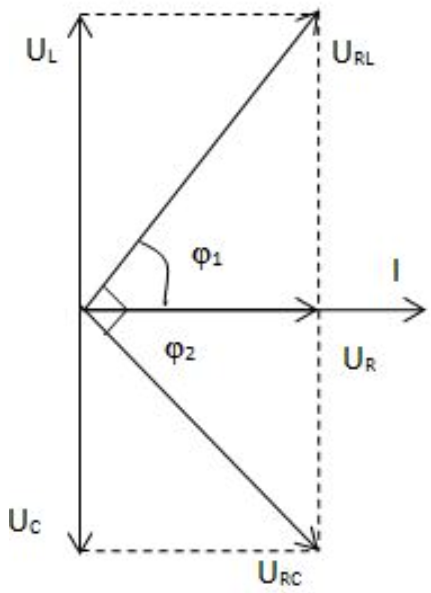
\includegraphics[scale=0.8]{../figs/VN12-2021-PH-TP024-3}
		\end{center}
	
		Ta có:
		$$\tan \varphi_1 \cdot \tan \varphi_2 = 1 \Rightarrow \dfrac{Z_L}{R} \cdot \dfrac{Z_C}{R} = 1 \Rightarrow R^2 = Z_L \cdot Z_C.$$
	}
	
	\item \mkstar{2}
	
	\cauhoi{
		Đoạn mạch $RLC$ mắc nối tiếp, cuộn dây thuần cảm. Gọi $U_R$, $U_L$, $U_C$ lần lượt là điện áp hiệu dụng ở hai đầu điện trở, cuộn cảm thuần và tụ điện. Biết $U_L = 2 U_R = 2 U_C$. Kết luận nào sau đây là đúng?
		
		\begin{mcq}(2)
			\item $u$ sớm pha hơn $i$ một góc $\dfrac{\pi}{4}\ \text{rad}$.
			\item $u$ chậm pha hơn $i$ một góc $\dfrac{\pi}{4}\ \text{rad}$.
			\item $u$ sớm pha hơn $i$ một góc $\dfrac{3\pi}{4}\ \text{rad}$.
			\item $u$ chậm pha hơn $i$ một góc $\dfrac{3\pi}{4}\ \text{rad}$.
		\end{mcq}
	}
	\loigiai{
		\textbf{Đáp án A.}
		
		Áp dụng $\tan \varphi = \dfrac{U_L - U_C}{U_R} = \dfrac{2U_R - U_R}{U_R} = 1$, suy ra $u$ sớm pha hơn $i$ một góc $\dfrac{\pi}{4}\ \text{rad}$.
	}
	
	\item \mkstar{2}
	
	\cauhoi{
		Cho đoạn mạch điện $RLC$ nối tiếp. Đặt vào hai đầu mạch một điện áp xoay chiều ổn định $u$ thì điện áp giữa hai đầu các phần tử là $U_R = \sqrt{3} U_C$, $U_L = 2 U_C$. Độ lệch pha giữa điện áp hai đầu đoạn mạch và cường độ dòng điện là
		
		\begin{mcq}(4)
			\item $\dfrac{\pi}{6}\ \text{rad}$.
			\item $-\dfrac{\pi}{6}\ \text{rad}$.
			\item $\dfrac{\pi}{3}\ \text{rad}$.
			\item $-\dfrac{\pi}{3}\ \text{rad}$.
		\end{mcq}
	}
	\loigiai{
		\textbf{Đáp án A.}
		
		Áp dụng $\tan \varphi = \dfrac{U_L - U_C}{U_R} = \dfrac{2U_C - U_C}{\sqrt{3} U_C} = \dfrac{1}{\sqrt{3}}$, suy ra $u$ sớm pha hơn $i$ một góc $\dfrac{\pi}{6}\ \text{rad}$.
	}
	
	\item \mkstar{2}
	
	\cauhoi{
		Cho đoạn mạch $RLC$ mắc nối tiếp ($L$ là cuộn dây thuần cảm). Điện áp hiệu dụng giữa hai bản tụ điện là $U_C = \SI{160}{V}$, hai đầu đoạn mạch là $U=\SI{160}{V}$. Điện áp trên tụ điện lệch pha so với điện áp hai đầu đoạn mạch là $\dfrac{\pi}{3}\ \text{rad}$. Điện áp hiệu dụng giữa hai đầu cuộn cảm là
		
		\begin{mcq}(4)
			\item $\SI{80}{V}$.
			\item $\xsi{40\sqrt{3}}{V}$.
			\item $\SI{120}{V}$.
			\item $\SI{90}{V}$.
		\end{mcq}
	}
	\loigiai{
		\textbf{Đáp án A.}
		
		Dựa vào giản đồ vectơ:
		\begin{center}
			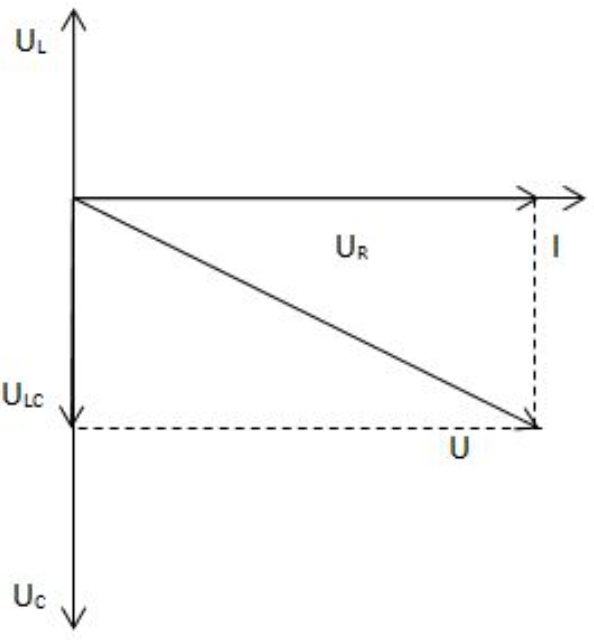
\includegraphics[scale=0.8]{../figs/VN12-2021-PH-TP024-4}
		\end{center}
	
		Ta có:
		$$U_{LC} = U \cos \dfrac{\pi}{3} = \dfrac{U}{2} = \SI{80}{V}.$$
		
		Điện áp hiệu dụng giữa hai đầu cuộn cảm:
		$$U_L = U_C - U_{LC} = \SI{80}{V}.$$
	}
	
	\item \mkstar{2}
	
	\cauhoi{
		Một đoạn mạch gồm cuộn dây có điện trở trong $R=\xsi{100\sqrt{3}}{\Omega}$, độ tự cảm $L$ mắc nối tiếp với tụ điện có điện dung $C=\xsi{\dfrac{5\cdot 10^{-5}}{\pi}}{F}$. Đặt vào hai đầu đoạn mạch một hiệu điện thế xoay chiều $u=U_0 \cos \left(100 \pi t - \dfrac{\pi}{4}\right)\ \text V$ thì cường độ dòng điện tức thời trong mạch là $i=\sqrt{2} \cos \left(100 \pi t - \dfrac{\pi}{12}\right)\ \text A$. Độ tự cảm của cuộn dây là
		
		\begin{mcq}(4)
			\item $\xsi{\dfrac{0,4}{\pi}}{H}$.
			\item $\xsi{\dfrac{0,5}{\pi}}{H}$.
			\item $\xsi{\dfrac{0,6}{\pi}}{H}$.
			\item $\xsi{\dfrac{1}{\pi}}{H}$.
		\end{mcq}
	}
	\loigiai{
		\textbf{Đáp án D.}
		
		Dung kháng của tụ điện:
		$$Z_C = \dfrac{1}{\omega C} = \SI{200}{\Omega}.$$
		
		Ta có $\varphi = \varphi_u - \varphi_i = \xsi{-\dfrac{\pi}{6}}{rad}$, suy ra:
		$$\tan \varphi = \dfrac{Z_L - Z_C}{R} = \tan (-\dfrac{\pi}{6}) = - \dfrac{\sqrt{3}}{3} \Rightarrow Z_L = \SI{100}{\Omega}.$$
		
		Vậy $L=\dfrac{Z_L}{\omega} = \xsi{\dfrac{1}{\pi}}{H}$.
	}
	
	\item \mkstar{3}
	
	\cauhoi{
		Một đoạn mạch gồm điện trở $R=\SI{100}{\Omega}$ mắc nối tiếp với tụ điện có điện dung $C=\dfrac{10^{-4}}{\pi}\ \text F$. Đặt vào hai đầu mạch một điện áp xoay chiều $u=200 \cos (100\pi t)\ \text V$. Cường độ dòng điện hiệu dụng qua mạch là
		
		\begin{mcq}(4)
			\item $\xsi{1,2\sqrt{2}}{A}$.
			\item $\SI{1}{A}$.
			\item $\SI{2}{A}$.
			\item $\xsi{\sqrt{2}}{A}$.
		\end{mcq}
	}
	\loigiai{
		\textbf{Đáp án B.}
		
		Trở kháng toàn mạch:
		$$Z = \sqrt{R^2 + Z_C^2} = \SI{100}{\Omega}.$$
		
		Cường độ dòng điện hiệu dụng toàn mạch:
		$$I=\dfrac{U}{Z} = \SI{1}{A}.$$
	}
	
	\item \mkstar{3}
	
	\cauhoi{
		Một mạch điện gồm điện trở thuần $R=\SI{100}{\Omega}$ mắc nối tiếp với cuộn cảm thuần có độ tự cảm $L=\dfrac{1}{\pi}\ \text H$. Đặt vào hai đầu đoạn mạch một điện áp xoay chiều $u=200 \cos(100\pi t)\ \text V$. Công suất tiêu thụ của mạch điện là
		
		\begin{mcq}(4)
			\item $\xsi{200\sqrt{2}}{W}$.
			\item $\SI{200}{W}$.
			\item $\SI{100}{W}$.
			\item $\SI{50}{W}$.
		\end{mcq}
	}
	\loigiai{
		\textbf{Đáp án C.}
		
		Trở kháng toàn mạch:
		$$Z=\sqrt{R^2 + Z_L^2} = \xsi{100\sqrt{2}}{\Omega}.$$
		
		Cường độ dòng điện hiệu dụng toàn mạch:
		$$I=\dfrac{U}{Z} = \SI{1}{A}.$$
		
		Công suất tiêu thụ:
		$$\calP = I^2 R = \SI{100}{W}.$$
	}
	
	\item \mkstar{3}
	
	\cauhoi{
		Cho một đoạn mạch điện xoay chiều gồm các đoạn mắc nối tiếp nhau: đoạn AM chứa tụ điện, đoạn MN chứa cuộn cảm thuần, đoạn NB chứa điện trở thuần. Biết $U_\text{AM} = \SI{40}{V}$, $U_\text{MB} = \xsi{20\sqrt 2}{V}$, $U_\text{AB} = \xsi{20\sqrt{2}}{V}$. Hệ số công suất của mạch bằng
		
		\begin{mcq}(4)
			\item $\dfrac{\sqrt{2}}{2}$.
			\item $\dfrac{1}{2}$.
			\item $\sqrt{2}$.
			\item $\dfrac{1}{4}$.
		\end{mcq}
	}
	\loigiai{
		\textbf{Đáp án A.}
		
		Ta có $U_C = U_\text{AM}$, $U_L = U_\text{MN}$, $U_R = U_\text{NB}$, $U_{RL} = U_\text{MB}$.
		
		Mặt khác, ta có $U_{RL}^2 = U_R^2 + U_L^2$ và $U_\text{AB}^2 = U_R^2 + U_L^2 + U_C^2 - 2 U_L U_C$.
		
		Suy ra $U_C^2 = 2 U_L U_C \Rightarrow U_L =\dfrac{U_C}{2} = \SI{20}{V}$ và $U_R=\SI{20}{V}$.
		
		Vậy hệ số công suất là
		$$\cos \varphi = \dfrac{U_R}{U_\text{AB}} = \dfrac{\sqrt{2}}{2}.$$
	}
	
	\item \mkstar{3}
	
	\cauhoi{
		Cho đoạn mạch xoay chiều $RLC$ nối tiếp. Biết điện áp đặt vào hai đầu đoạn mạch là $u=100 \cos 100 \pi t\ \text V$, điện áp hiệu dụng giữa hai đầu cuộn cảm thuần là $U_L = \SI{50}{V}$, công suất tiêu thụ trên đoạn mạch $\calP = \SI{50}{W}$ và dòng điện sớm pha $\dfrac{\pi}{4}\ \text{rad}$ so với điện áp. Điện trở $R$ và dung kháng $Z_C$ có giá trị là
		
		\begin{mcq}(2)
			\item $R=\SI{100}{\Omega}$, $Z_C = \SI{50}{\Omega}$.
			\item $R=\SI{50}{\Omega}$, $Z_C = \SI{50}{\Omega}$.
			\item $R=\SI{50}{\Omega}$, $Z_C = \SI{100}{\Omega}$.
			\item $R=\SI{100}{\Omega}$, $Z_C = \SI{100}{\Omega}$.
		\end{mcq}
	}
	\loigiai{
		\textbf{Đáp án C.}
		
		Ta có $\tan \varphi = \dfrac{U_L - U_C}{U_R} = \tan \dfrac{\pi}{4} = 1$. Suy ra $U_L - U_C = U_R$.
		
		Với $\calP = UI \cos \varphi = \SI{50}{W}$, trong đó $U=\sqrt{U_R^2 + (U_L - U_C)^2} = \sqrt{2U_R^2}$ và $I=\dfrac{U_R}{R}$. Tính được $R=\SI{50}{\Omega}$ và $Z_C = \SI{100}{\Omega}$.
	}
	
	\item \mkstar{3}
	
	\cauhoi{
		Cho đoạn mạch điện xoay chiều gồm điện trở thuần $R$ và tụ điện có điện dung $C=\dfrac{10^{-4}}{3\pi}\ \text F$ mắc vào mạch điện xoay chiều có giá trị điện áp hiệu dụng $\SI{150}{V}$, tần số $\SI{50}{Hz}$ và cường độ dòng điện trong mạch có giá trị hiệu dụng là $\dfrac{\sqrt{5}}{5}\ \text{A}$. Điện trở thuần $R$ có giá trị bằng
		
		\begin{mcq}(4)
			\item $\SI{50}{\Omega}$.
			\item $\SI{150}{\Omega}$.
			\item $\SI{200}{\Omega}$.
			\item $\SI{100}{\Omega}$.
		\end{mcq}
	}
	\loigiai{
		\textbf{Đáp án B.}
		
		Dung kháng của tụ điện:
		$$Z_C = \dfrac{1}{\omega C} = \SI{300}{\Omega}.$$
		
		Trở káng của toàn mạch:
		$$Z=\sqrt{R^2  + Z_C^2} = \dfrac{U}{I} = \xsi{150\sqrt{5}}{\Omega}.$$
		
		Suy ra $R=\SI{150}{\Omega}$.
	}
	
	\item \mkstar{3}
	
	\cauhoi{
		Cho mạch điện $RLC$ như hình vẽ.
		\begin{center}
			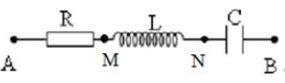
\includegraphics[scale=1]{../figs/VN12-2021-PH-TP024-1.png}
		\end{center}
		
		Cho điện áp hai đầu mạch là $u_\text{AB} = 200 \sqrt{2} \cos 100 \pi t\ \text{V}$ và điện trở $R=\xsi{100\sqrt{3}}{\Omega}$. Điện áp hai đầu đoạn mạch MN nhanh pha hơn hiệu điện thế hai đầu mạch AB một góc $\xsi{\dfrac{2\pi}{3}}{rad}$. Cường độ dòng điện $i$ qua mạch có biểu thức:
		\begin{mcq}(2)
			\item $i=\sqrt{2} \cos \left(100 \pi t + \dfrac{\pi}{6}\right)\ \text A$.
			\item $i=\sqrt{2} \cos \left(100 \pi t + \dfrac{\pi}{3}\right)\ \text A$.
			\item $i=\sqrt{2} \cos \left(100 \pi t - \dfrac{\pi}{3}\right)\ \text A$.
			\item $i=\sqrt{2} \cos \left(100 \pi t - \dfrac{\pi}{6}\right)\ \text A$.
		\end{mcq}
	}
	\loigiai{
		\textbf{Đáp án A.}
		
		Giả sử cuộn dây là thuần cảm, ta có giản đồ vectơ:
		\begin{center}
			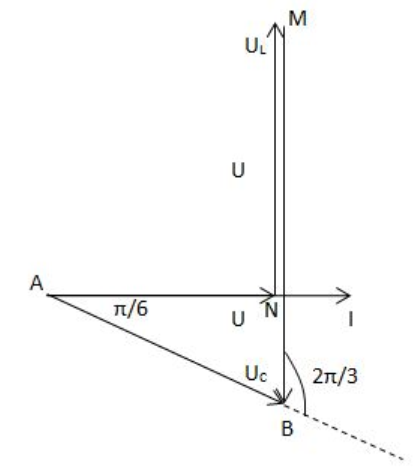
\includegraphics[scale=0.8]{../figs/VN12-2021-PH-TP024-5}
		\end{center}
	
		Xét tam giác vuông NAB, có: $\text{AB} = \dfrac{\text{AN}}{\cos \dfrac{\pi}{6}} = \dfrac{2}{\sqrt{3}} \text{AN}$, hay $Z=\dfrac{2}{\sqrt{3}} R = \SI{200}{\Omega}$.
		
		Cường độ dòng điện cực đại:
		$$I_0 = \dfrac{U_0}{Z} = \xsi{\sqrt{2}}{A}.$$
		
		Vì $i$ sớm pha hơn $u$ một góc $\dfrac{\pi}{6}\ \text{rad}$, nên biểu thức của $i$ là
		$$i=\sqrt{2} \cos \left(100 \pi t + \dfrac{\pi}{6}\right)\ \text{A}.$$
	}
	
	\item \mkstar{3}
	
	\cauhoi{
		Cho mạch điện như hình vẽ.
		\begin{center}
			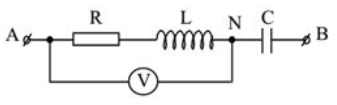
\includegraphics[scale=1]{../figs/VN12-2021-PH-TP024-2.png}
		\end{center}
	
	Với $U_\text{AB} = \SI{300}{V}$, $U_\text{NB} = \SI{140}{V}$, dòng điện $i$ trễ pha so với $u_\text{AB}$ một góc $\varphi$ (với $\cos \varphi = \SI{0.8}{}$), cuộn dây thuần cảm. Vôn kế V chỉ giá trị
		\begin{mcq}(4)
			\item $\SI{100}{V}$.
			\item $\SI{200}{V}$.
			\item $\SI{300}{V}$.
			\item $\SI{400}{V}$.
		\end{mcq}
	}
	\loigiai{
		\textbf{Đáp án D.}
		
		Ta có giản đồ vectơ:
		\begin{center}
			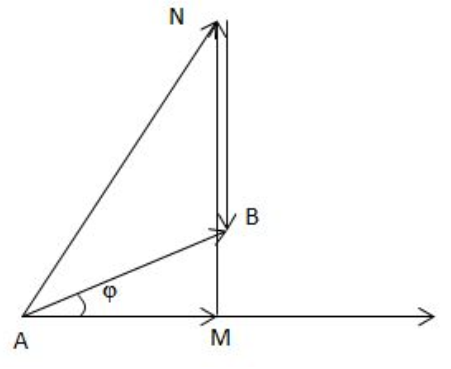
\includegraphics[scale=0.8]{../figs/VN12-2021-PH-TP024-6}
		\end{center}
	
	Trong tam giác vuông MAB có $\widehat{\text{MBA}} = \varphi = 90^\circ$, suy ra $\cos \varphi = \sin \widehat{\text{MBA}} = \SI{0.8}{}$.
	
	Mà lại có $\widehat{\text{MBA}} + \widehat{\text{ABN}} = 180^\circ$, suy ra: $\sin \widehat{\text{ABN}} = \sin \widehat{\text{MBA}} = \SI{0.8}{}$.
	
	Do đó $\cos \widehat{\text{ABN}} = \pm \sqrt{1 - \sin^2 \widehat{\text{ABN}}} = \pm \SI{0.6}{}$.
	
	Vì $\widehat{\text{ABN}}$ là góc tù nên $\cos \widehat{\text{ABN}} = \SI{-0.6}{}$.
	
	Trong tam giác ABN có: $\text{AN}^2 = \text{AB}^2 + \text{BN}^2 - 2 \cdot \text{AB} \cdot \text{BN} \cos \widehat{\text{ABN}}$, hay
	$$U_\text{AN}^2 = U_\text{AB}^2 + U_\text{NB}^2 - 2 U_\text{AB} U_\text{NB} \cos \widehat{\text{ABN}}.$$
	
	Thay số, ta được: $U_\text{AN} = \SI{400}{V}$.
	}
	
	\item \mkstar{3}
	
	\cauhoi{
		Mạch điện xoay chiều gồm điện trở thuần $R=\SI{30}{\Omega}$ mắc nối tiếp với cuộn dây. Đặt vào hai đầu mạch một điện áp xoay chiều $u=U\sqrt{2} \cos (100 \pi t)\ \text V$. Điện áp hiệu dụng ở hai đầu cuộn dây là $U_\text{d} = \SI{60}{V}$. Dòng điện trong mạch lệch pha $\dfrac{\pi}{6}\ \text{rad}$ so với $u$ và lệch pha $\dfrac{\pi}{3}\ \text{rad}$ so với $u_\text{d}$. Điện áp hiệu dụng ở hai đầu mạch có giá trị là
		
		\begin{mcq}(4)
			\item $U=\xsi{60\sqrt{2}}{V}$.
			\item $U=\SI{120}{V}$.
			\item $U=\SI{90}{V}$.
			\item $U=\xsi{60\sqrt{3}}{V}$.
		\end{mcq}
	}
	\loigiai{
		\textbf{Đáp án D.}
		
		Do dòng điện trong mạch lệch pha $\dfrac{\pi}{3}\ \text{rad}$ so với $u_\text{d}$ nên cuộn dây không thuần cảm. Giản đồ vectơ:
		\begin{center}
			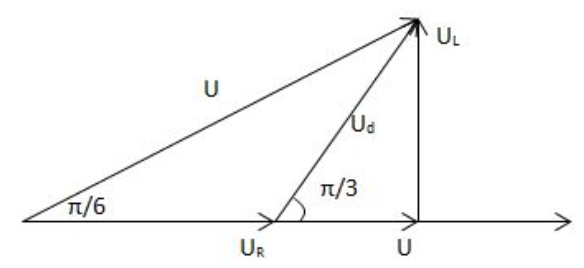
\includegraphics[scale=0.8]{../figs/VN12-2021-PH-TP024-7}
		\end{center}
	
	Ta có:
	$$U_\text{d} = U_R = \SI{60}{V}.$$
	$$U^2 = U_R^2 + U_\text{d}^2 - 2 U_R U_\text{d} \cos \dfrac{2\pi}{3}$$
	
	Thay số, ta được: $U=\xsi{60\sqrt 3}{V}$.
	}
	
	\item \mkstar{3}
	
	\cauhoi{
		Cho đoạn mạch điện xoay chiều gồm điện trở $R$, cuộn cảm thuần có độ tự cảm $L=\dfrac{0,2}{\pi}\ \text H$ và tụ điện $C=\dfrac{10^{-4}}{\pi}$ mắc nối tiếp. Đặt vào hai đầu đoạn mạch một điện áp xoay chiều có giá trị hiệu dụng $U=\SI{200}{V}$, tần số $\SI{50}{Hz}$. Để công suất tiêu thụ trên đoạn mạch là $\calP = \SI{240}{W}$ thì giá trị của điện trở là
		
		\begin{mcq}(2)
			\item $\SI{60}{\Omega}$ hoặc $\SI{160}{\Omega}$.
			\item $\SI{60}{\Omega}$ hoặc $\SI{106.7}{\Omega}$.
			\item $\SI{60}{\Omega}$ hoặc $\SI{30}{\Omega}$.
			\item $\SI{60}{\Omega}$ hoặc $\SI{180}{\Omega}$.
		\end{mcq}
	}
	\loigiai{
		\textbf{Đáp án B.}
		
		Công suất:
		$$\calP = I^2 R = \dfrac{U^2}{R^2 + (Z_L - Z_C)^2} R \Rightarrow \calP R^2 - U^2 R + \calP(Z_L - Z_C)^2 = 0$$
		$$\Rightarrow 240R^2 - 40000R + 1536000 = 0$$
		
		Vậy $R=\SI{60}{\Omega}$ hoặc $R=\SI{106.67}{\Omega}$.
		
	}
	
	\item \mkstar{3}
	
	\cauhoi{
		Cho đoạn mạch xoay chiều $RLC$ nối tiếp. Đặt vào hai đầu đoạn mạch điện áp $u=100\sqrt{2} \cos 100 \pi t\ \text V$. Biết công suất tiêu thụ trên đoạn mạch là $\SI{100}{W}$, dòng điện chạy trong mạch nhanh hơn điện áp một góc $\dfrac{\pi}{4}$ và điện áp hiệu dụng giữa hai đầu cuộn cảm thuần là $\xsi{50\sqrt{2}}{V}$. Điện dung $C$ của tụ điện có giá trị bằng
		
		\begin{mcq}(4)
			\item $\dfrac{4\cdot10^{-4}}{\pi}\ \text F$.
			\item $\dfrac{2\cdot 10^{-4}}{\pi}\ \text F$.
			\item $\dfrac{10^{-4}}{\pi}\ \text F$.
			\item $\SI{26.38}{F}$.
		\end{mcq}
	}
	\loigiai{
		\textbf{Đáp án C.}
		
		Ta có $\tan \varphi = \dfrac{U_L - U_C}{R} =\tan \dfrac{\pi}{4} = 1$, suy ra $U_L - U_C = U_R$.
		
		Vì $u=\sqrt{U_R^2 + (U_L - U_C)^2} = \sqrt{2 (U_L - U_C)^2}$, suy ra $U_L - U_C = 50\sqrt{2}$.
		
		Tính được: $U_C = \xsi{100\sqrt{2}}{V}$ và $U_R = \xsi{50\sqrt 2}{V}$.
		
		Mà $\calP = U_R I$, suy ra:
		$$I = \dfrac{\calP}{U_R} = \xsi{\sqrt{2}}{A}.$$
		
		Vậy $Z_C = \dfrac{U_C}{I} = \SI{100}{\Omega}$ hay $C=\dfrac{1}{\omega C} = \dfrac{10^{-4}}{\pi}\ \text{F}$.
	}
	
	\item \mkstar{3}
	
	\cauhoi{
		Một đoạn mạch xoay chiều gồm hai trong ba phần tử mắc nối tiếp: điện trở thuần $R$, tụ điện có dung kháng $Z_C$, cuộn cảm có cảm kháng $Z_L$. Biết điện áp xoay chiều giữa hai đầu đoạn mạch là $u=120 \sqrt{2} \cos (100\pi t)\ \text V$. Cường độ dòng điện qua mạch có biểu thức $i=1,2 \cos \left(100 \pi t - \dfrac{\pi}{4}\right)\ \text A$. Thông số của hai phần tử đó là
		
		\begin{mcq}(2)
			\item $R=Z_L = \SI{100}{\Omega}$.
			\item $R=Z_C = \SI{100}{\Omega}$.
			\item $Z_L = Z_C = \xsi{25\sqrt{2}}{\Omega}$.
			\item $R=Z_L = \xsi{25\sqrt{2}}{\Omega}$.
		\end{mcq}
	}
	\loigiai{
		\textbf{Đáp án A.}
		
		Vì $u$ sớm pha hơn $i$ nên đoạn mạch gồm hai phần tử nối tiếp: $R$ và $L$. Khi đó:
		$$Z=\sqrt{R^2 + Z_L^2} = \dfrac{U}{I} = \xsi{100\sqrt 2}{\Omega}.$$
		
		Mà $\tan \varphi = \dfrac{Z_L}{R} = \tan \dfrac{\pi}{4} = 1$, nên $R=Z_L = \SI{100}{\Omega}$.
	}
	
	\item \mkstar{3}
	
	\cauhoi{
		Cho đoạn mạch xoay chiều $RLC$ nối tiếp, trong đó $L$ thay đổi được. Điện áp đặt vào hai đầu đoạn mạch có biểu thức $u=200 \sqrt{2} \cos 100 \pi t \ \text V$. Biết khi $L=L_1 = \dfrac{3\sqrt{3}}{\pi}\ \text H$ và khi $L=L_2 = \dfrac{\sqrt{3}}{\pi}\ \text{H}$ thì cường độ dòng điện hiệu dụng chạy trong đoạn mạch đều bằng nhau, nhưng giá trị tức thời lệch pha nhau một góc là $\dfrac{2\pi}{3}\ \text{rad}$. Điện trở $R$ có giá trị bằng
		
		\begin{mcq}(4)
			\item $\xsi{200\sqrt{3}}{\Omega}$.
			\item $\SI{200}{\Omega}$.
			\item $\xsi{100\sqrt{3}}{\Omega}$.
			\item $\SI{100}{\Omega}$.
		\end{mcq}
	}
	\loigiai{
		\textbf{Đáp án D.}
		
		Vì khi $L = L_1$ hoặc $L=L_2$ thì $i_1 = i_2 = i$ nên ta có $Z_1 = Z_2$. Khi đó:
		$$Z_C = \dfrac{Z_{L1} + Z_{L2}}{2} = \xsi{200\sqrt{3}}{\Omega}.$$
		
		Mặt khác, ta lại có:
		$$\tan (\varphi_1 + \varphi_2) = \dfrac{\tan \varphi_1 + \tan \varphi_2}{1 - \tan \varphi_1 \cdot \tan \varphi_2} = \tan \dfrac{2\pi}{3} = -\sqrt{3}.$$
		
		Thay $\tan \varphi_1 = \dfrac{Z_{L1} - Z_C}{R}$ và $\tan \varphi_2 = \dfrac{Z_C - Z_{L2}}{R}$, ta được $R=\SI{100}{\Omega}$.
	}
	
	\item \mkstar{3}
	
	\cauhoi{
		Cho một đoạn mạch điện xoay chiều gồm các đoạn mắc nối tiếp nhau: đoạn AM chứa tụ điện, đoạn MN chứa điện trở thuần, đoạn NB chứa cuộn cảm thuần. Biết $U_\text{AN} = \SI{200}{V}$, $U_\text{MB} = \SI{150}{V}$, điện áp tức thời $u_\text{AN}$ vuông pha với $u_\text{MB}$, cường độ dòng điện trong mạch có giá trị hiệu dụng $\SI{2}{A}$, tần số $\SI{50}{Hz}$. Độ tự cảm có giá trị bằng
		
		\begin{mcq}(4)
			\item $\dfrac{0,45}{\pi}\ \text{H}$.
			\item $\dfrac{1,45}{\pi}\ \text H$.
			\item $\SI{0,45}{H}$.
			\item $\SI{0.25}{H}$.
		\end{mcq}
	}
	\loigiai{
		\textbf{Đáp án A.}
		
		Trở kháng của đoạn AN là $Z_\text{AN} = \sqrt{R^2 + Z_C^2} = \dfrac{U_\text{AN}}{I} = \SI{100}{\Omega}$, suy ra:
		$$R^2 + Z_C^2 = 100^2.$$
		
		Trở kháng của đoạn MB là $Z_{MB} = \sqrt{R^2 + Z_L^2} = \dfrac{U_\text{MB}}{I} = \SI{75}{\Omega}$, suy ra:
		$$R^2 + Z_L^2 = 75^2.$$
		
		Mà $u_\text{AN}$ vuông pha với $u_\text{MB}$ nên:
		$$\tan \varphi_\text{AN} \cdot \tan \varphi_\text{MB} = 1 \Rightarrow \dfrac{Z_C}{R} \cdot \dfrac{Z_L}{R} = 1 \Rightarrow Z_L Z_C = R^2.$$
		
		Giải hệ 3 phương trình trên, tìm được $Z_L = \SI{45}{\Omega}$ hay $L=\dfrac{0,45}{\pi}\ \text{H}$.
	}
	
	\item \mkstar{3}
	
	\cauhoi{
		Cho đoạn mạch xoay chiều gồm các phần tử $R$, $L$, $C$ mắc nối tiếp, trong đó $R$ thay đổi được, $Z_L = \SI{15}{\Omega}$, $Z_C = \SI{4}{\Omega}$, điện áp đặt vào hai đầu đoạn mạch là $u=12\sqrt{2} \cos 100 \pi t \ \text V$. Công suất tiêu thụ của đoạn mạch đạt cực đại khi $R$ bằng
		
		\begin{mcq}(4)
			\item $\SI{11}{\Omega}$.
			\item $\SI{6}{\Omega}$.
			\item $\SI{2}{\Omega}$.
			\item $\SI{14}{\Omega}$.
		\end{mcq}
	}
	\loigiai{
		\textbf{Đáp án A.}
		
		$R$ thay đổi để $\calP_\text{max}$ khi $R=|Z_L - Z_C|$, khi đó $R=\SI{11}{\Omega}$.
	}
	
	\item \mkstar{3}
	
	\cauhoi{
		Cho mạch điện gồm $R$, $L$, $C$ mắc nối tiếp. Biết điện trở $R$ không thay đổi, hệ số tự cảm $L=\dfrac{0,5}{\pi}\ \text H$, tụ điện có điện dung $C$ thay đổi được. Đặt vào hai đầu đoạn mạch một điện áp ổn định có biểu thức $u=200 \sqrt{2} \cos (100\pi t)\ \text V$. Giá trị của $C$ để công suất tiêu thụ trong mạch đạt cực đại là
		
		\begin{mcq}(4)
			\item $\dfrac{0,1}{\pi}\ \text F$.
			\item $\dfrac{10^{-2}}{\pi}\ \text F$.
			\item $\dfrac{10^{-3}}{\pi}\ \text F$.
			\item $\dfrac{2\cdot 10^{-4}}{\pi}\ \text F$.
		\end{mcq}
	}
	\loigiai{
		\textbf{Đáp án D.}
		
		Thay đổi $C$ để $\calP_\text{max}$ thì trong mạch xảy ra cộng hưởng, khi đó:
		$$Z_L = Z_C \Rightarrow C = \dfrac{1}{\omega^2 L} = \dfrac{2 \cdot 10^{-4}}{\pi}\ \text{F}.$$
	}
	
	\item \mkstar{4}
	
	\cauhoi{
		Đặt điện áp xoay chiều có giá trị hiệu dụng không đổi $\SI{150}{V}$ vào đoạn mạch AMB gồm AM chỉ chứa điện trở $R$, đoạn MB chứa tụ điện có điện dung C mắc nối tiếp với một cuộn cảm thuần có độ tự cảm $L$ thay đổi được. Biết sau khi thay đổi độ tự cảm $L$ thì điện áp hiệu dụng hai đầu đoạn mạch MB tăng $2\sqrt{2}$ lần và dòng điện trong mạch trước sau thay đổi pha một góc $\dfrac{\pi}{2}\ \text{rad}$. Tìm điện áp hiêu jdụng hai đầu đoạn mạch AM khi chưa thay đổi $L$.
		
		\begin{mcq}(4)
			\item $\SI{100}{V}$.
			\item $\xsi{100\sqrt{2}}{V}$.
			\item $\xsi{100\sqrt{3}}{V}$.
			\item $\SI{120}{V}$.
		\end{mcq}
	}
	\loigiai{
		\textbf{Đáp án B.}
		
		Gọi $\varphi_1$, $\varphi_2$ lần lượt là độ lệch pha giữa $u$ và $i$ trước và sau khi thay đổi $L$.
		$$\tan \varphi_1 = \dfrac{U_{L1} - U_{C1}}{U_{R1}}$$
		$$\tan \varphi_2 = \dfrac{U_{L2} - U_{C2}}{U_{R2}}$$
		
		Ta có $i_1$ và $i_2$ vuông pha với nhau nên:
		$$\varphi_1 + \varphi_2 = \dfrac{\pi}{2} \Rightarrow \tan \varphi_1 \cdot \tan \varphi_2 = -1.$$
		
		Thay các đại lượng vào, ta được:
		$$(U_{L1} - U_{C1})^2 \cdot (U_{L2} - U_{C2})^2 = U_{R1}^2 U_{R2}^2 \Rightarrow 8 U_\text{MB1}^2 = U_{R1}^2 U_{R2}^2.$$
		
		Mặt khác:
		$$U_{R1}^2 + U_\text{MB1}^2 = U_{R2}^2 + U_\text{MB2}^2 = U^2 \Rightarrow U_{R2}^2 = U_{R1}^2 - 7 U_\text{MB1}^2.$$
		
		Suy ra $8 U_\text{MB1}^2 = U_{R1}^2 \cdot (U_{R1}^2 - 7 U_\text{MB1}^2)$, hay:
		$$U_{R1}^2 = 8 U_\text{MB1}^2.$$
		
		Ngoài ra thì $U_{R1}^2 + U_\text{MB1}^2 = U^2$. Tính được:
		$$U_{R1} = 2 \cdot \dfrac{\sqrt{2}}{3} \cdot U = \xsi{100\sqrt{2}}{V}.$$
	}
	
	\item \mkstar{4}
	
	\cauhoi{
		Một đoạn mạch AB gồm 3 phần tử $R$, $L$, $C$ mắc nối tiếp (cuộn dây thuần cảm có độ tự cảm $L$). Đặt điện áp xoay chiều $u=U\sqrt{2} \cos 2\pi f t\ \text V$ ($U$ không đổi, $f$ thay đổi được) vào hai đầu đoạn mạch AB. Khi tần số là $f=f_0$ thì dòng điện sớm pha $\dfrac{\pi}{4}\ \text{rad}$ so với điện áp hai đầu mạch AB và lúc đó cảm kháng bằng với giá trị của $R$. Khi tần số là $f=f_1 = 2f_0$ thì độ lệch pha giữa điện áp hai đầu mạch AB so với cường độ dòng điện là
		
		\begin{mcq}(4)
			\item $\dfrac{\pi}{3}\ \text{rad}$.
			\item $\dfrac{\pi}{4}\ \text{rad}$.
			\item $\dfrac{\pi}{6}\ \text{rad}$.
			\item $-\dfrac{\pi}{4}\ \text{rad}$.
		\end{mcq}
	}
	\loigiai{
		\textbf{Đáp án B.}
		
		Sử dụng phương pháp chuẩn hóa số liệu, cho $Z_L = R = 1$ khi $f=f_0$.
		
		Khi $f=f_0$, dòng điện sớm pha $\dfrac{\pi}{4}\ \text{rad}$ so với điện áp hai đầu đoạn mach:
		$$\tan (-\dfrac{\pi}{4}) = \dfrac{Z_{L0} - Z_{C0}}{R} = -1 \Rightarrow Z_{C0} - Z_{L0} = R = 1 \Rightarrow Z_{C0} = 2.$$
		
		Khi $f=f_1=2f_0$ thì $Z_{L1} = 2 Z_{L0} = 2$ và $Z_{C1} = 1$:
		$$\tan \varphi_1 = \dfrac{Z_{L1} - Z_{C1}}{R} = 1.$$
		
		Vậy $\varphi_1 = \dfrac{\pi}{4}\ \text{rad}$.
	}
	
	\item \mkstar{4}
	
	\cauhoi{
		Đặt điện áp $u=U\sqrt{2} \cos 2\pi f t\ \text{V}$ ($U$ không đổi, $f$ thay đổi được) vào hai đầu đoạn mạch mắc nối tiếp gồm điện trở thuần $R$, cuộn cảm thuần có độ tự cảm $L$ và tụ điện có điện dung $C$. Khi tần số là $f_1$ thì cảm kháng và dung kháng của đoạn mạch có giá trị lần lượt là $\SI{6}{\Omega}$ và $\SI{8}{\Omega}$. Khi tần số là $f_2$ thì hệ số công suất của đoạn mạch bằng 1. Hệ thức liên hệ giữa $f_1$ và $f_2$ là
		
		\begin{mcq}(2)
			\item $f_2 =\dfrac{4}{3} f_1$.
			\item $f_2 = \dfrac{\sqrt{3}}{2} f_1$.
			\item $f_2 = \dfrac{2}{\sqrt{3}} f_1$.
			\item $f_2 = \dfrac{3}{4} f_1$.
		\end{mcq}
	}
	\loigiai{
		\textbf{Đáp án C.}
		
		Giả sử $f_2 = n f_1$, ta có:
		$$Z_{L1} = 6 \Rightarrow Z_{L2} = 6n.$$
		$$Z_{C1} = 8 \Rightarrow Z_{C2} = \dfrac{8}{n}.$$
		
		Theo đề, khi tần số là $f_2$ thì $\cos \varphi = 1$, khi đó có hiện tượng cộng hưởng nên $Z_{L2} = Z_{C2}$, hay $6n = \dfrac{8}{n}$, vậy $n=\dfrac{2}{\sqrt{3}}$.
		
		Vậy $f_2 = \dfrac{2}{\sqrt{3}}f_1$.
	}
	
	\item \mkstar{4}
	
	\cauhoi{
		Đặt vào hai đầu cuộn sơ cấp của một máy biến áp lí tưởng (bỏ qua hao phí) một điện áp xoay chiều có giá trị hiệu dụng không đổi thì điện áp hiệu dụng giữa hai đầu cuộn thứ cấp để hở là $\SI{100}{V}$. Ở cuộn thứ cấp, nếu giảm bớt $n$ vòng dây thì điện áp giữa hai đầu để hở của nó là $U$, nếu tăng thêm $n$ vòng dây thì điện áp đó là $2U$. Nếu tăng thêm $3n$ vòng dây ở cuộn thứ cấp thì điện áp hiệu dụng giữa hai đầu để hở của cuộn này bằng
		
		\begin{mcq}(4)
			\item $\SI{100}{V}$.
			\item $\SI{200}{V}$.
			\item $\SI{220}{V}$.
			\item $\SI{110}{V}$.
		\end{mcq}
	}
	\loigiai{
		\textbf{Đáp án B.}
		
		Tỉ số giữa điện áp và số vòng dây ở hai đầu cuộn sơ cấp và thứ cấp:
		$$\dfrac{100}{U_1} = \dfrac{N_2}{N_1}\ (*).$$
		
		Tỉ số giữa điện áp và số vòng dây ở hai đầu cuộn sơ cấp và thứ cấp:
		$$\dfrac{U}{U_1} = \dfrac{N_2 - n}{N_1}\ (**).$$
		
		Tỉ số giữa điện áp và số vòng dây ở hai đầu cuộn sơ cấp và thứ cấp:
		$$\dfrac{2U}{U_1} = \dfrac{N_2 + n}{N_1}\ (***).$$
		
		Lấy $(**)$ cộng $(***)$ và thay $(*)$ vào, suy ra:
		$$\dfrac{2N_2}{N_1} = \dfrac{3U}{U_1} = \dfrac{200}{U_1} \Rightarrow U = \dfrac{200}{3}\ \text{V}.$$
		
		Lấy $(***)$ trừ $(**)$, suy ra:
		$$\dfrac{U}{U_1} = \dfrac{2n}{N_1} \Rightarrow \dfrac{1}{2} \dfrac{U}{U_1} = \dfrac{n}{N_1}.$$
		
		Nếu tăng thêm $3n$ vòng dây thì:
		$$\dfrac{U_2}{U_1} = \dfrac{N_2 + 3n}{N_1} = \dfrac{N_2}{N_1} + 3 \dfrac{n}{N_1} = \dfrac{100}{U_1} + 3 \cdot\dfrac{1}{2} \cdot \dfrac{\frac{200}{3}}{U_1} = \dfrac{200}{U_1}.$$
		
		Suy ra: $U_2 = \SI{200}{V}$.
	}
	
	\item \mkstar{4}
	
	\cauhoi{
		Một máy phát điện xoay chiều ba pha đang hoạt động ổn định. Suất điện động trong ba cuộn dây của phần ứng có giá trị $e_1$, $e_2$ và $e_3$. Ở thời điểm mà $e_1 = \SI{30}{V}$ thì $|e_2 - e_3| = \SI{30}{V}$. Giá trị cực đại của $e_1$ là
		
		\begin{mcq}(4)
			\item $\SI{40.2}{V}$.
			\item $\SI{51.9}{V}$.
			\item $\SI{34.6}{V}$.
			\item $\SI{45.1}{V}$.
		\end{mcq}
	}
	\loigiai{
		\textbf{Đáp án C.}
		
		Giả sử suất điện động trong khung dây có dạng:
		$$
		\begin{cases}
			e_1 = E_0 \cos \omega t \\
			e_2 = E_0 \cos \left(\omega t + \dfrac{2\pi}{3}\right)\\
			e_3 =E_0 \cos \left(\omega t - \dfrac{2\pi}{3}\right)
		\end{cases}
		$$
		
		Theo đề bài:
		$$|e_2 - e_3| = \SI{30}{V} \Rightarrow e_2 - e_3 = \pm \SI{30}{V} \Rightarrow 2 E_0 \sin \omega t \sin \dfrac{2\pi}{3} = \pm \SI{30}{V}.$$
		
		Ngoài ra, cũng theo đề bài:
		$$e_1 = E_0 \cos \omega t = \SI{30}{V}.$$
		
		Ta có hệ phương trình sau:
		$$
		\begin{cases}
			-2E_0 \sin \omega t \sin \dfrac{2\pi}{3} = \pm \SI{30}{V}\\
			E_0 \cos \omega t = \SI{30}{V}
		\end{cases}
		\Rightarrow
		\begin{cases}
			E_0 \sin \omega t = \pm \xsi{10\sqrt{3}}{V}\\
			E_0 \cos \omega t = \SI{30}{V}
		\end{cases}
	\Rightarrow E_0 = \xsi{20\sqrt{3}}{V}=\SI{34.6}{V}.
		$$
	}
\end{enumerate}
\loigiai{\textbf{Đáp án}
	\begin{center}
		\begin{tabular}{|m{2.8em}|m{2.8em}|m{2.8em}|m{2.8em}|m{2.8em}|m{2.8em}|m{2.8em}|m{2.8em}|m{2.8em}|m{2.8em}|}
			\hline
			1. B & 2. C & 3. D & 4. B & 5. B & 6. D & 7. C & 8. D & 9. A & 10. B \\
			\hline
			11. B & 12. D & 13. B & 14. A & 15. A & 16. D & 17. A & 18. A & 19. A & 20. D\\
			\hline
			21. B & 22. C & 23. A & 24. C & 25. B & 26. A & 27. D & 28. D & 29. B & 30. C\\
			\hline
			31. A & 32. D & 33. A & 34. A & 35. D & 36. B & 37. B & 38. C & 39. B & 40. C\\
			\hline
		\end{tabular}
\end{center}}
	\stopcontents[mychapters]

	
\setcounter{mychapter}{24}
	\mychapter{Giao thoa ánh sáng}
	\startcontents[mychapters]
	\printcontents[mychapters]{}{0}{\setcounter{tocdepth}{1}}
	\whiteBGstarBegin
\setcounter{section}{0}
\section{Lý thuyết: Giao thoa ánh sáng và điều kiện xảy ra giao thoa ánh sáng}
\begin{enumerate}[label=\bfseries Câu \arabic*:]

%========================================
    \item \mkstar{1} [5]
    
	\cauhoi
	{Trong thí nghiệm Y-âng, tại vị trí vân tối thì
		\begin{mcq}(1)
			\item Độ lệch pha của hai sóng từ hai nguồn kết hợp thỏa mãn $\delta \varphi = (2k+1) \dfrac{\pi}{2}$ với $k \in Z$. 
			\item Hai sóng đến từ hai nguồn kết hợp vuông pha với nhau. 
			\item Hiệu quang trình từ hai nguồn kết hợp thỏa mãn $d_{2} - d_{1} = (2k+1)\dfrac{\lambda}{2}$ với $k \in Z$. 
			\item Hiệu quang trình từ hai nguồn kết hợp thỏa mãn $d_{2} - d_{1} = (2k+1)\lambda$ với $k \in Z$.  
		\end{mcq}
	}
	
	\loigiai
	{		\textbf{Đáp án:  C.}
		
Trong thí nghiệm Y-âng, tại vị trí vân tối thì hiệu quang trình từ hai nguồn kết hợp thỏa mãn $d_{2} - d_{1} = (2k+1)\dfrac{\lambda}{2}$ với $k \in Z$. 
		
	}

%========================================
    \item \mkstar{1} [5]
    
	\cauhoi
	{Hiện tượng giao thoa chứng tỏ rằng 
		\begin{mcq}(2)
			\item ánh sáng là sóng ngang. 
			\item ánh sáng là sóng điện từ. 
			\item ánh sáng có bản chất sóng. 
			\item ánh sáng có thể bị tán sắc. 
		\end{mcq}
	}
	
	\loigiai
	{		\textbf{Đáp án: C.}
		
Hiện tượng giao thoa chứng tỏ rằng ánh sáng có bản chất sóng.
		
	}

%========================================
    \item \mkstar{1} [5]
    
	\cauhoi
	{Hiện tượng giao thoa ánh sáng chỉ quan sát được khi hai nguồn ánh sáng là hai nguồn 
		\begin{mcq}(2)
			\item cùng màu sắc. 
			\item đơn sắc. 
			\item cùng cường độ. 
			\item kết hợp. 
		\end{mcq}
	}
	
	\loigiai
	{		\textbf{Đáp án: D.}
		
Hiện tượng giao thoa ánh sáng chỉ quan sát được khi hai nguồn ánh sáng là hai nguồn kết hợp.
		
	}

%========================================
    \item \mkstar{1} [13]
    
	\cauhoi
	{Trong thí nghiệm Y-âng về giao thoa ánh sáng, với k là số nguyên. Công thức dùng để xác định vị trí vân sáng trên màn quan sát là
		\begin{mcq}(2)
			\item $x = \dfrac{a}{D} k \lambda$. 
			\item $x = \dfrac{D}{2a} \lambda$. 
			\item $x= k \dfrac{\lambda D}{a}$. 
			\item $x = \dfrac{D}{a} (k+0,5) \lambda$. 
		\end{mcq}
	}
	
	\loigiai
	{		\textbf{Đáp án: C.}
		
Công thức xác định vị trí vân sáng trong giao thoa khe Y-âng là $x= k \dfrac{\lambda D}{a}$.
		
	}

%========================================
    \item \mkstar{1} [10]
    
	\cauhoi
	{Hiện tượng giao thoa ánh sáng là bằng chứng thực nghiệm chứng tỏ ánh sáng
		\begin{mcq}(2)
			\item là sóng siêu âm. 
			\item có tính chất sóng. 
			\item là sóng dọc. 
			\item có tính chất hạt. 
		\end{mcq}
	}
	
	\loigiai
	{		\textbf{Đáp án: B.}
		
Hiện tượng giao thoa ánh sáng là bằng chứng thực nghiệm chứng tỏ ánh sáng có tính chất sóng.
		
	}

%========================================
    \item \mkstar{1} [3]
    
	\cauhoi
	{Trong thí nghiệm giao thoa ánh sáng khe Young, điều kiện để có hiện tượng giao thoa ánh sáng trên màn quan sát thì sóng ánh sáng do hai nguồn thứ cấp $S_{1}$ và $S_{2}$ phải
		\begin{mcq}(1)
			\item cùng phương, cùng biên độ nhưng có hiệu số pha thay đổi theo thời gian. 
			\item cùng tần số nhưng có hiệu số pha thay đổi theo thời gian. 
			\item cùng biên độ nhưng khác tần số dao động. 
			\item cùng phương, cùng tần số và có hiệu số pha không thay đổi theo thời gian. 
		\end{mcq}
	}
	
	\loigiai
	{		\textbf{Đáp án: D.}

Điều kiện để xảy ra giao thoa là hai nguồn thứ cấp $S_{1}$ và $S_{2}$ phải cùng phương, cùng tần số và có hiệu số pha không thay đổi theo thời gian.
		
	}

%========================================
    \item \mkstar{1} [1]
    
	\cauhoi
	{Hiện tượng nào sau đây liên quan đến tính chất sóng của ánh sáng?
		\begin{mcq}(2)
			\item Hiện tượng quang dẫn. 
			\item Hiện tượng quang phát quang. 
			\item Hiện tượng quang điện trong. 
			\item Hiện tượng giao thoa ánh sáng. 
		\end{mcq}
	}
	
	\loigiai
	{		\textbf{Đáp án: D.}
		
Hiện tượng giao thoa là đặc trưng cho tính chất sóng của ánh sáng.
		
	}
	
%========================================
    \item \mkstar{1} [2]
    
	\cauhoi
	{Điều khẳng định nào sau đây là \textbf{sai} khi nói về bản chất sóng của ánh sáng?
		\begin{mcq}(1)
			\item Ánh sáng có lưỡng tính sóng - hạt. 
			\item Khi tính chất hạt rõ nét, ta dễ quan sát hiện tượng giao thoa ánh sáng. 
			\item Khi ánh sáng có bước sóng càng ngắn, thì khả năng đâm xuyên càng mạnh. 
			\item Khi ánh sáng có bước sóng càng ngắn, thì tính chất hạt càng thể hiện rõ, tính chất sóng càng ít thể hiện. 
		\end{mcq}
	}
	
	\loigiai
	{		\textbf{Đáp án: B.}
		
Khi tính chất hạt rõ nét, ta khó quan sát hiện tượng giao thoa ánh sáng.
		
	}
%========================================
    \item \mkstar{1} [9]
    
	\cauhoi
	{Thực hiện thí nghiệm Y-âng về giao thoa ánh sáng đơn sắc màu đỏ ta quan sát được hệ vân giao thoa trên màn. Nếu thay ánh sáng đơn sắc màu đỏ bằng ánh sáng đơn sắc màu lục và các điều khác của thí nghiệm được giữ nguyên thì 
		\begin{mcq}(2)
			\item khoảng vân tăng lên. 
			\item khoảng vân không thay đổi. 
			\item vị trí vân trung tâm thay đổi. 
			\item khoảng vân giảm xuống. 
		\end{mcq}
	}
	
	\loigiai
	{		\textbf{Đáp án: D.}
		
Khi thay ánh sáng đơn sắc màu đỏ bằng ánh sáng đơn sắc màu lục thì bước sóng giảm xuống. Vì khoảng vân tỉ lệ với bước sóng nên khoảng vân cũng giảm xuống.
		
	}	

\end{enumerate}

\loigiai
{
	\begin{center}
		\textbf{BẢNG ĐÁP ÁN}
	\end{center}
	\begin{center}
		\begin{tabular}{|m{2.8em}|m{2.8em}|m{2.8em}|m{2.8em}|m{2.8em}|m{2.8em}|m{2.8em}|m{2.8em}|m{2.8em}|m{2.8em}|}
			\hline
			01.C  & 02.C  & 03.D  & 04.C  & 05.B  & 06.D  & 07.D & 08.B & 09.D & \\
			\hline
			
		\end{tabular}
	\end{center}
}

\section{Dạng bài: Giao thoa ánh sáng đơn sắc}
\begin{enumerate}[label=\bfseries Câu \arabic*:]
	
%========================================
\item \mkstar{3} [13]

\cauhoi
{Trong thí nghiệm Y-âng về giao thoa ánh sáng. Khi tiến hành trong không khí, người ta đo được khoảng vân là $i = \SI{2}{mm}$. Tiến hành thí nghiệm trong nước, nước có chiết suất tuyệt đối là $n = \dfrac{4}{3}$ thì khoảng vân đo được trong nước là
	\begin{mcq}(4)
		\item $\SI{2,5}{mm}$. 
		\item $\SI{2}{mm}$. 
		\item $\SI{1,5}{mm}$. 
		\item $\SI{1,25}{mm}$. 
	\end{mcq}
}

\loigiai
{		\textbf{Đáp án: C.}
	
	Gọi $i'$ là khoảng vân đo được trong môi trường nước. Ta có
	$$
	i' = \dfrac{i}{n} = \SI{1,5}{mm}.
	$$
}

%========================================
\item \mkstar{3} [9]

\cauhoi
{Trong thí nghiệm Y-âng về giao thoa ánh sáng đơn sắc, khoảng cách giữa hai khe là $\SI{1}{mm}$, khoảng cách từ mặt phẳng chứa hai khe đến màn là $\SI{2}{m}$. Trong hệ vân trên màn, vân sáng bậc 3 cách vân trung tâm là $\SI{2,4}{mm}$. Bước sóng của ánh sáng đơn sắc dùng trong thí nghiệm là 
	\begin{mcq}(4)
		\item $\SI{0,5}{\mu m}$. 
		\item $\SI{0,7}{\mu m}$. 
		\item $\SI{0,4}{\mu m}$. 
		\item $\SI{0,6}{\mu m}$. 
	\end{mcq}
}

\loigiai
{		\textbf{Đáp án: C.}
	
	Vân sáng bậc 3 cách vân trung tâm $3i$ nên
	$$
	3i = \SI{2,4}{mm} \rightarrow i = \SI{0,8}{mm}.
	$$
	Ta có
	$$
	i = \dfrac{\lambda D}{a} \rightarrow \lambda = \SI{0,4}{\mu m}.
	$$
}
	
%========================================
\item \mkstar{3} [9]

\cauhoi
{Thực hiện giao thoa ánh sáng theo khe Y-âng với $a = \SI{2}{mm}$, $D= \SI{1}{m}$, nguồn S phát ra ánh sáng đơn sắc có bước sóng $\lambda = \SI{0,5}{\mu m}$. Khoảng cách từ vân sáng bậc 5 đến vân tối bậc 7 ở hai bên vân sáng trung tâm là
	\begin{mcq}(4)
		\item $\SI{2,875}{mm}$. 
		\item $\SI{11,5}{mm}$. 
		\item $\SI{2,6}{mm}$. 
		\item $\SI{12,5}{mm}$. 
	\end{mcq}
}

\loigiai
{		\textbf{Đáp án: A.}
	
	Khoảng cách giữa vân sáng bậc 5 và vân tối bậc 7 ở hai phía so với vân trung tâm là
	$$
	5i + 6,5i = 11,5i = 11,5 \dfrac{\lambda D}{a} = \SI{2,875}{mm}.
	$$
}
	
%========================================
\item \mkstar{3} [9]

\cauhoi
{Trong thí nghiệm Y-âng về giao thoa ánh sáng đơn sắc, người ta đo được khoảng cách từ vân sáng bậc 2 đến vân sáng bậc 5 cùng một phía so với vân trung tâm là $\SI{3}{mm}$. Số vân sáng quan sát được trên MN đối xứng với nhau qua vân sáng trung tâm có bề rộng là $\SI{13}{mm}$ là
	\begin{mcq}(4)
		\item 9 vân. 
		\item 13 vân. 
		\item 15 vân. 
		\item 11 vân. 
	\end{mcq}
}

\loigiai
{		\textbf{Đáp án: B.}
	
	Khoảng cách từ vân sáng bậc 2 đến vân sáng bậc 5 là $3i$ nên
	$$
	3i = \SI{3}{mm} \rightarrow i = \SI{1}{mm}.
	$$
	Ta có:
	$$
	\dfrac{L}{2i} = \num{6,5}.
	$$
	Số vân sáng trên đoạn MN là 13 vân.
}
	
%========================================
\item \mkstar{3} [23]

\cauhoi
{ Trong thí nghiệm giao thoa khe Y-âng, khoảng cách giữa hai vân sáng cạnh nhau là
	
	\begin{mcq}(4)
		\item $\dfrac{\lambda}{aD}$. 
		\item $\dfrac{ax}{D}$. 
		\item $\dfrac{\lambda a}{D}$. 
		\item $\dfrac{\lambda D}{a}$. 
	\end{mcq}
}

\loigiai
{		\textbf{Đáp án: D.}
	
	Khoảng cách giữa hai vân sáng cạnh nhau là khoảng vân $i = \dfrac{\lambda D}{a}$.		
}
	
%========================================
\item \mkstar{3} [13]

\cauhoi
{Trong một thí nghiệm Y-âng về giao thoa ánh sáng, bước sóng ánh sáng đơn sắc là $\lambda$ (m). Khoảng cách giữa hai khe hẹp là $a$ (m. Khoảng cách từ mặt phẳng phân cách chứa hai khe đến màn là $D$ (m). Vị trí vân tối có tọa độ $x_{k}$ là
	\begin{mcq}(2)
		\item $x_{k} = (2k+1)\dfrac{\lambda D}{a}$. 
		\item $x_{k} = k \dfrac{\lambda D}{a}$. 
		\item $x_{k} = (2k+1) \dfrac{\lambda D}{2a}$. 
		\item $x_{k} = k \dfrac{\lambda D}{2a}$. 
	\end{mcq}
}

\loigiai
{		\textbf{Đáp án: C.}
	
	Vị trí vân tối là 
	$$
	x_{k} = (2k+1) \dfrac{\lambda D}{2a}.
	$$
}
	
%========================================
\item \mkstar{3} [7]

\cauhoi
{Trong thí nghiệm Y-âng về giao thoa ánh sáng, hai khe được chiếu bằng ánh sáng đơn sắc có bước sóng $\SI{0,6}{\mu m}$, khoảng cách giữa hai khe hẹp là $\SI{1}{mm}$, khoảng cách từ mặt phẳng chứa hai khe đến màn quan sát là $\SI{2,5}{m}$. Khoảng vân giao thoa trên màn là
	
	\begin{mcq}(4)
		\item $\SI{1,5}{mm}$.
		\item $\SI{1,0}{mm}$. 	
		\item $\SI{2,0}{mm}$.  	
		\item $\SI{0,5}{mm}$. 
	\end{mcq}
}

\loigiai
{		\textbf{Đáp án: A.}
	
	Khoảng vân trên màn cho bởi
	$$
	i = \dfrac{\lambda D}{a} = \SI{1,5}{mm}.
	$$
}

	
%========================================
\item \mkstar{3} [5]

\cauhoi
{Trong thí nghiệm giao thoa khe Y-âng, nguồn sóng có bước sóng là $\SI{380}{nm}$.  Khoảng cách giữa hai khe hẹp là $\SI{2}{mm}$. Khoảng cách giữa hai khe đến màn là $\SI{2}{m}$. Khoảng vân là
	\begin{mcq}(4)
		\item $\SI{3}{mm}$. 
		\item $\SI{0,38}{mm}$. 
		\item $\SI{0,62}{mm}$. 
		\item $\SI{0,54}{mm}$. 
	\end{mcq}
}

\loigiai
{		\textbf{Đáp án: B.}
	
	Khoảng vân của hệ cho bởi
	$$
	i = \dfrac{\lambda D}{a} = \SI{0,38}{mm}.
	$$
}
	
%========================================
\item \mkstar{3} [5]

\cauhoi
{Khi thực hiện giao thoa với ánh sáng đơn sắc, nếu hai khe Y-âng cách nhau $\SI{1,2}{mm}$ thì khoảng vân là $i = \SI{1,21}{mm}$. Nếu khoảng cách giữa hai khe giảm đi $\SI{0,2}{mm}$ thì khoảng vân sẽ 
	\begin{mcq}(2)
		\item giảm đi $\SI{0,24}{mm}$. 
		\item giảm đi $\SI{0,11}{mm}$. 
		\item tăng thêm $\SI{0,24}{mm}$. 
		\item tăng thêm $\SI{0,11}{mm}$. 
	\end{mcq}
}

\loigiai
{		\textbf{Đáp án: C.}
	
	Ta có:
	$$
	\dfrac{i'}{i} = \dfrac{a}{a'} = \dfrac{a}{a- \Delta a} \rightarrow i' = \SI{1,452}{mm}.
	$$
	Như vậy khoảng vân sẽ tăng thêm $\SI{0,24}{mm}$.
}
	
%========================================
\item \mkstar{3} [13]

\cauhoi
{Trong thí nghiệm Y-âng về giao thoa ánh sáng có $\lambda = \SI{0,75}{\mu m}$, $a = \SI{0,6}{mm}$ và $D = \SI{1,2}{m}$. Tại điểm M trên màn quan sát cách vân trung tâm $\SI{5,25}{mm}$ có vân
	\begin{mcq}(2)
		\item sáng bậc 3. 
		\item tối thứ 3. 
		\item tối thứ 4. 
		\item sáng bậc 4. 
	\end{mcq}
}

\loigiai
{		\textbf{Đáp án: C.}
	
	Khoảng vân $i$ là
	$$
	i = \dfrac{\lambda D}{a} = \SI{1,5}{mm}. 
	$$
	Ta có:
	$$
	\dfrac{x}{i} = 3,5.
	$$
	Vậy tại $x = \SI{5,25}{mm}$ là vân tối thứ 4.
}
	
%========================================
\item \mkstar{3} [13]

\cauhoi
{Trong thí nghiệm Y-âng về giao thoa ánh sáng có $a = \SI{1}{mm}$ và $D = \SI{1}{m}$. Trên màn quan sát ta thấy vân sáng bậc 5 cách vân sáng trung tâm là $\SI{3,0}{mm}$. Bước sóng ánh sáng dùng trong thí nghiệm là
	\begin{mcq}(4)
		\item $\lambda = \SI{0,70}{\mu m}$. 
		\item $\lambda = \SI{0,50}{\mu m}$. 
		\item $\lambda = \SI{0,60}{\mu m}$. 
		\item $\lambda = \SI{0,53}{\mu m}$. 
	\end{mcq}
}

\loigiai
{		\textbf{Đáp án: C.}
	
	Khoảng cách từ vân sáng bậc 5 đến vân sáng trung tâm là
	$$
	\Delta d = 5i \rightarrow  i = \SI{0,6}{mm}.
	$$
	Khoảng vân cho bởi
	$$
	i = \dfrac{\lambda D}{a} \rightarrow \lambda = \SI{0,60}{\mu m}.
	$$
}

%========================================
\item \mkstar{3} [13]

\cauhoi
{Trong thí nghiệm Y-âng về giao thoa ánh sáng với khoảng vân là $i$, khoảng cách từ vân sáng bậc 3 đến vân sáng bậc 7 ở cùng một phía so với vân sáng trung tâm là 
	\begin{mcq}(4)
		\item $3i$. 
		\item $4i$. 
		\item $7i$. 
		\item $5i$. 
	\end{mcq}
}

\loigiai
{		\textbf{Đáp án: B.}
	
	Khoảng cách giữa vân sáng bậc 3 và vân sáng bậc 7 cho bởi
	$$
	\Delta d = 7i - 3i = 4i.
	$$
}
	
%========================================
\item \mkstar{3} [13]

\cauhoi
{Trong thí nghiệm Y-âng về giao thoa ánh sáng có $\lambda = \SI{0,5}{\mu m}$, $a = \SI{1,2}{mm}$ và $D = \SI{2,5}{m}$. Vân tối thứ ba cách vân trung tâm một khoảng bằng
	\begin{mcq}(4)
		\item $\SI{2,1}{mm}$. 
		\item $\SI{3,1}{mm}$. 
		\item $\SI{2,6}{mm}$. 
		\item $\SI{3,6}{mm}$. 
	\end{mcq}
}

\loigiai
{		\textbf{Đáp án: C.}
	
	Vân tối thứ ba cách vân trung tâm một đoạn là
	$$
	x_{t_{3}} = 2,5i = 2,5 \dfrac{\lambda D}{a} = \SI{2,6}{mm}.
	$$
}
	
%========================================
\item \mkstar{3} [13]

\cauhoi
{Trong thí nghiệm Y-âng về giao thoa ánh sáng có $\lambda = \SI{0,5}{\mu m}$, $a = \SI{1}{mm}$ và $D = \SI{2}{m}$. Khoảng vân $i$ bằng
	\begin{mcq}(4)
		\item $\SI{2,5}{mm}$. 
		\item $\SI{5,0}{mm}$. 
		\item $\SI{2,0}{mm}$. 
		\item $\SI{1,0}{mm}$. 
	\end{mcq}
}

\loigiai
{		\textbf{Đáp án: D.}
	
	Khoảng vân $i$ là
	$$
	i = \dfrac{\lambda D}{a} = \SI{1,0}{mm}.
	$$
}

%========================================
\item \mkstar{3} [13]

\cauhoi
{Trong thí nghiệm về giao thoa ánh sáng có $\lambda = \SI{0,7}{\mu m}$, $a = \SI{0,35}{mm}$ và $D = \SI{1}{m}$. Bề rộng của trường giao thoa là $L = \SI{18,2}{mm}$. Số vân sáng quan sát được là
	\begin{mcq}(4)
		\item $11$. 
		\item $8$. 
		\item $10$. 
		\item $9$. 
	\end{mcq}
}

\loigiai
{		\textbf{Đáp án: D.}
	
	Khoảng vân là
	$$
	i = \dfrac{\lambda D}{a} = \SI{2}{mm}.
	$$
	Ta có
	$$
	\dfrac{L}{2i} = \num{4,55}.
	$$
	Số vân quan sát được là 9 vân.
}
	
%========================================
\item \mkstar{3} [13]

\cauhoi
{Đoạn MN trên màn quan sát trong thí nghiệm Y-âng về giao thoa ánh sáng. Khi dùng ánh sáng có bước sóng $\lambda$ thì khoảng cách giữa hai vân sáng liên tiếp là $\SI{1,2}{mm}$. Trên MN có 16 vân sáng quan sát được (tại M, N đều là vân sáng). Đoạn MN có giá trị là
	\begin{mcq}(4)
		\item $\SI{10}{mm}$. 
		\item $\SI{12}{mm}$. 
		\item $\SI{16}{mm}$. 
		\item $\SI{18}{mm}$. 
	\end{mcq}
}

\loigiai
{		\textbf{Đáp án: D.}
	
	Khoảng cách giữa hai vân sáng liên tiếp cũng là khoảng vân nên $i = \SI{1,2}{mm}$.
	Tại M và N là các vân sáng và trên MN có tổng cộng 16 vân sáng quan sát được thì
	$$
	MN = 15i = \SI{18}{mm}.
	$$
}
%========================================
\item \mkstar{3} [12]

\cauhoi
{Thực hiện thí nghiệm Y-âng về giao thoa ánh sáng với khoảng cách giữa hai khe sáng là $\SI{2}{mm}$, khoảng cách từ mặt phẳng chứa hai khe đến màn quan sát là $\SI{2}{m}$, ánh sáng đơn sắc có bước sóng $\SI{0,7}{\mu m}$. Khoảng cách giữa vân sáng và vân tối liền kề là 
	
	\begin{mcq}(4)
		\item $\SI{0,0875}{mm}$. 
		\item $\SI{0,3500}{mm}$.
		\item $\SI{0,7000}{mm}$.
		\item $\SI{0,1750}{mm}$.
	\end{mcq} 
}

\loigiai
{		\textbf{Đáp án: B.}
	
	Khoảng cách giữa vân sáng và vân tối liền kề là $\num{0,5} i = \num{0,5} \dfrac{\lambda D}{a} = \SI{0,3500}{mm}$.		
}

%========================================
\item \mkstar{3} [12]

\cauhoi
{Thực hiện thí nghiệm Y-âng với ánh sáng đơn sắc có bước sóng $\lambda$. Biết khoảng cách giữa hai khe là $a$, khoảng cách từ mặt phẳng chứa hai khe đến màn quan sát là $D$ thì vân sáng bậc 3 cách vân trung tâm 
	\begin{mcq}(4)
		\item $4 \dfrac{\lambda D}{a}$. 
		\item $3 \dfrac{\lambda a}{D}$. 
		\item $3 \dfrac{\lambda D}{a}$. 
		\item $4 \dfrac{\lambda a}{D}$. 
	\end{mcq}
}

\loigiai
{		\textbf{Đáp án: C.}
	
	Vân sáng bậc 3 cách vân trung tâm một khoảng là $3 \dfrac{\lambda D}{a}$.	
}

%========================================
\item \mkstar{3 } [12]

\cauhoi
{Khoảng cách giữa 2 vân sáng liền kề là $\SI{0,5}{mm}$ thì khoảng vân có giá trị 
	\begin{mcq}(4)
		\item $\SI{1,5}{mm}$.
		\item $\SI{1,0}{mm}$. 
		\item $\SI{0,5}{mm}$.
		\item $\SI{0,25}{mm}$.
	\end{mcq}
}

\loigiai
{		\textbf{Đáp án: C.}
	
	Khoảng cách giữa 2 vân sáng liền kề là $\SI{0,5}{mm}$ thì khoảng vân cũng có giá trị $\SI{0,5}{mm}$.	
}
	
%========================================
\item \mkstar{3} [10]

\cauhoi
{Trong thí nghiệm Y-âng về giao thoa với ánh sáng đơn sắc, khoảng cách giữa hai khe là $\SI{1}{mm}$, khoảng cách từ mặt phẳng chứa hai khe đến màn quan sát là $\SI{2}{m}$ và khoảng vân là $\SI{0,8}{mm}$. Cho $c = 3 \cdot 10^{8} \; \si{m/s}$. Tần số ánh sáng đơn sắc dùng trong thí nghiệm là
	
	\begin{mcq}(4)
		\item $\text{5,5} \cdot 10^{14} \si{Hz}$. 
		\item $\text{4,5} \cdot 10^{14} \si{Hz}$. 
		\item $\text{7,5} \cdot 10^{14} \si{Hz}$.
		\item $\text{6,5} \cdot 10^{14} \si{Hz}$. 
	\end{mcq}
}

\loigiai
{		\textbf{Đáp án: C.}
	
	Khoảng vân cho bởi
	$$
	i = \dfrac{\lambda D}{a}  \rightarrow \lambda = \SI{0,4}{\mu m}
	$$
	Tần số ánh sáng cho bởi
	$$
	f = \dfrac{c}{\lambda} = \SI{7,5 e14}{Hz}.
	$$
}
	%========================================
	\item \mkstar{3} [10]
	
	\cauhoi
	{Trong thí nghiệm Y-âng về giao thoa ánh sáng, nguồn sáng phát ra ánh sáng đơn sắc có bước sóng $\SI{500}{nm}$. Khoảng cách giữa hai khe là $\SI{1}{mm}$, khoảng cách từ mặt phẳng chứa hai khe đến màn quan sát là $\SI{1}{m}$. Trên màn, khoảng cách giữa hai vân sáng liên tiếp bằng
		\begin{mcq}(4)
			\item $\SI{0,50}{mm}$.
			\item $\SI{1,0}{mm}$.
			\item $\SI{1,5}{mm}$. 
			\item $\SI{0,75}{mm}$. 
		\end{mcq}
	}
	
	\loigiai
	{		\textbf{Đáp án: A.}
		
		Khoảng cách giữa hai vân sáng là
		$$
		i = \dfrac{\lambda D}{a} = \SI{0,5}{mm}.
		$$
	}
	
%========================================
\item \mkstar{3} [4]

\cauhoi
{Trong thí nghiệm Y-âng về giao thoa ánh sáng đơn sắc có bước sóng $\lambda = \SI{0,6}{\mu m}$. Khoảng cách giữa hai khe là $\SI{1}{mm}$, khoảng cách từ hai khe đến màn là $\SI{2}{m}$. Vân sáng thứ tư cách vân trung tâm một khoảng là
	\begin{mcq}(4)
		\item $\SI{4,2}{mm}$. 
		\item $\SI{3,6}{mm}$. 
		\item $\SI{4,8}{mm}$. 
		\item $\SI{6,0}{mm}$. 
	\end{mcq}
}

\loigiai
{		\textbf{Đáp án: C.}
	
	Vân sáng thứ tư cách vân trung tâm một khoảng là
	$$
	x_{4} = 4 \dfrac{\lambda D}{a} = \SI{4,8}{mm}.
	$$
}

%========================================
\item \mkstar{3} [4]

\cauhoi
{Trong thí nghiệm Y-âng về giao thoa ánh sáng, hai khe cách nhau $\SI{3}{mm}$ được chiếu bằng ánh sáng đơn sắc có bước sóng $\SI{0,6}{\mu m}$. Các vân giao thoa được hứng trên màn cách hai khe $\SI{2}{m}$. Tại điểm M cách vân trung tâm $\SI{1,2}{mm}$ có
	\begin{mcq}(2)
		\item vân sáng bậc 3. 
		\item vân tối thứ 3. 
		\item vân sáng bậc 5. 
		\item vân sáng bậc 4. 
	\end{mcq}
}

\loigiai
{		\textbf{Đáp án: A.}
	
	Khoảng vân là $i = \dfrac{\lambda D}{a} = \SI{0,4}{mm}$.
	Tại điểm M, ta có:
	$$
	\dfrac{x_{M}}{i} = 3.
	$$
	Vậy tại M là vân sáng bậc 3.
}
	
%========================================
\item \mkstar{3} [2]

\cauhoi
{Trong thí nghiệm Y-âng về giao thoa ánh sáng đơn sắc, ta thấy tại điểm M trên màn có vân sáng bậc 5. Dịch chuyển màn quan sát ra xa thêm $\SI{20}{cm}$ thì tại M có vân tối thứ 5 tính từ trung tâm. Trước lúc dịch chuyển, khoảng cách từ màn đến hai khe bằng
	\begin{mcq}(4)
		\item $\SI{2}{m}$. 
		\item $\SI{1,8}{m}$. 
		\item $\SI{1,6}{m}$. 
		\item $\SI{2,2}{m}$. 
	\end{mcq}
}

\loigiai
{		\textbf{Đáp án: B.}
	
	Ban đầu, vị trí của điểm M cho bởi
	$$
	x_{M} = 5 \dfrac{\lambda D}{a}.
	$$
	Lúc sau, vị trí điểm M cho bởi
	$$
	x_{M} = \num{4,5} \dfrac{\lambda (D + \Delta D)}{a}.
	$$
	Từ hai phương trình trên ta được:
	$$
	5D = \num{4,5}(D + \Delta D) \rightarrow D = \SI{1,8}{m}.
	$$
}
	

%========================================
\item \mkstar{3} [3]

\cauhoi
{Trong thí nghiệm Y-âng về giao thoa ánh sáng, hai khe được chiếu bằng ánh sáng đơn sắc có bước sóng $\lambda$. Khoảng cách giữa hai khe sáng là $a$, khoảng cách từ mặt phẳng chứa hai khe đến màn quan sát là $\SI{1}{m}$. Trên màn quan sát, hai vân sáng bậc 3 nằm ở hai điểm M và N. Dịch màn quan sát một đoạn $\SI{50}{cm}$ theo hướng ra xa 2 khe thì số vân sáng trên đoạn MN giảm so với lúc đầu là 
	\begin{mcq}(4)
		\item 2 vân. 
		\item 5 vân. 
		\item 7 vân. 
		\item 4 vân. 
	\end{mcq}
}

\loigiai
{		\textbf{Đáp án: A.}
	
	Vì tại M và N là vị trí vân sáng bậc 3 ở hai bên vân trung tâm nên $\text{MN} = 6i$.
	Ta có:
	$$
	\dfrac{i'}{i} = \dfrac{D'}{D} = \dfrac{D + \Delta D}{D} = 1,5 \rightarrow i' = 1,5i.
	$$
	Ta có:
	$$
	\dfrac{\text{MN}}{2i'} = \dfrac{6i}{3i} = 2 \rightarrow MN = 2i'.
	$$
	Vậy số vân sáng trên đoạn MN lúc sau là 5 vân, giảm 2 vân so với lúc đầu là 7 vân.
}

%=========================================
\item \mkstar{3} [1]

\cauhoi
{Trong thí nghiệm Y-âng về giao thoa ánh sáng, hai khe được chiếu bằng ánh sáng đơn sắc. Khoảng cách giữa hai khe là $\SI{1,2}{mm}$. Khoảng cách từ mặt phẳng chứa hai khe đến màn quan sát là $\SI{1,5}{m}$. Trên màn quan sát, xét đoạn gồm 6 vân sáng liên tiếp cạnh nhau thì hai vân sáng ngoài cùng cách nhau $\SI{3}{mm}$. Bước sóng của ánh sáng đơn sắc này bằng
	\begin{mcq}(4)
		\item $\SI{600}{nm}$. 
		\item $\SI{400}{nm}$. 
		\item $\SI{500}{nm}$. 
		\item $\SI{480}{nm}$. 
	\end{mcq}
}

\loigiai
{		\textbf{Đáp án: D.}
	
	Độ rộng của 6 vân sáng liên tiếp là $5i$, suy ra $i = \SI{0,6}{mm}$.
	Khoảng vân cho bởi:
	$$
	i = \dfrac{\lambda D}{a} \rightarrow \lambda = \SI{480}{nm}.
	$$
}

%========================================
\item \mkstar{3} [13]

\cauhoi
{Trong thí nghiệm Y-âng về giao thoa ánh sáng có $a = \SI{1}{mm}$ và $D = \SI{1}{m}$. Trên màn quan sát thấy vân sáng bậc 5 cách vân sáng trung tâm $\SI{3,0}{mm}$. Bước sóng ánh sáng đơn sắc dùng trong thí nghiệm là
	\begin{mcq}(4)
		\item $\lambda = \SI{0,70}{\mu m}$. 
		\item $\lambda = \SI{0,50}{\mu m}$. 
		\item $\lambda = \SI{0,60}{\mu m}$. 
		\item $\lambda = \SI{0,53}{\mu m}$. 
	\end{mcq}
}

\loigiai
{		\textbf{Đáp án: C.}
	
Vị trí của vân sáng bậc 5 cho bởi:
	$$
	x_{5} = 5 \dfrac{\lambda D}{a} \rightarrow \lambda = \SI{0,6}{\mu m}.
	$$
}
	
%========================================
\item \mkstar{3} [1]

\cauhoi
{Trong thí nghiệm Y-âng về giao thoa ánh sáng, hai khe được chiếu bằng ánh sáng đơn sắc có bước sóng $\SI{0,48}{\mu m}$. Khoảng cách giữa hai khe là $\SI{0.9}{mm}$, khoảng cách từ mặt phẳng chứa hai khe đến màn quan sát là $\SI{1,5}{m}$. Trên màn quan sát, so với vân sáng trung tâm, vân tối thứ ba cách vân sáng trung tâm
	\begin{mcq}(4)
		\item $\SI{2,8}{mm}$. 
		\item $\SI{2,4}{mm}$. 
		\item $\SI{2}{mm}$. 
		\item $\SI{1,6}{mm}$. 
	\end{mcq}
}

\loigiai
{		\textbf{Đáp án: C.}

	Khoảng vân cho bởi
	$$
	i = \dfrac{\lambda D}{a} = \SI{0,8}{mm}.
	$$
	Khoảng cách từ vân trung tâm tới vân tối thứ ba là $2,5i = \SI{2}{mm}$.
}

%========================================
\item \mkstar{4} [32]

\cauhoi
{Trong thí nghiệm Y-âng về giao thoa ánh sáng đơn sắc. Khoảng cách giữa hai khe là $\SI{1}{mm}$ và khoảng cách từ hai khe tới màn quan sát là $\SI{2}{m}$. Trong khoảng bề rộng $\SI{24,5}{mm}$ trên màn quan sát có 25 vân tối. Biết một đầu bề rộng là vân tối, đầu còn lại là vân sáng. Bước sóng của ánh sáng đó là
	\begin{mcq}(4)
		\item $\SI{0,48}{\mu m}$. 
		\item $\SI{0,40}{\mu m}$. 
		\item $\SI{0,50}{\mu m}$. 
		\item $\SI{0,52}{\mu m}$. 
	\end{mcq}
}

\loigiai
{		\textbf{Đáp án: C.}
	
	Một khoảng bề rộng có một đầu là vân sáng, đầu còn lại là vân tối với 25 vân tối thì bề rộng này có kích thước là $24,5i$. Ta có:
	$$
	\num{24,5}i = \SI{24,5}{mm} \rightarrow i = \SI{1}{mm}.
	$$
	Ta có:
	$$
	i = \dfrac{\lambda D}{a} \rightarrow \lambda = \SI{0,50}{\mu m}.
	$$
}

%========================================
\item \mkstar{4} [4]

\cauhoi
{Trong thí nghiệm Y-âng về giao thoa ánh có bước sóng $\lambda$, khoảng cách giữa hai khe là $\SI{1}{mm}$. Ban đầu, tại M cách vị trí trung tâm $\SI{5,25}{mm}$ người ta quan sát được vân sáng bậc 5. Giữ cố định màn chứa hai khe, di chuyển màn quan sát ra xa và dọc theo đường vuông góc với mặt phẳng chứa hai khe một đoạn $\SI{0,75}{m}$ thì ta thấy điểm M chuyển thành vân tối lần thứ hai. Bước sóng $\lambda$ có giá trị là
	\begin{mcq}(4)
		\item $\SI{0,60}{\mu m}$. 
		\item $\SI{0,50}{\mu m}$. 
		\item $\SI{0,70}{\mu m}$. 
		\item $\SI{0,64}{\mu m}$. 
	\end{mcq}
}

\loigiai
{		\textbf{Đáp án: A.}
	
	Vì khoảng cách từ hai khe đến màn tăng lên nên vị trí điểm M sẽ bị dời về vị trí các vân tối gần vân trung tâm hơn. Vì trong quá trình này, vị trí điểm M bị chuyển thành vân tối hai lần nên nó ở vị trí vân tối thứ 4.
	
	Tại vị trí điểm M lúc đầu và lúc sau, ta có:
	$$
	x_{M} = 5 \dfrac{\lambda D}{a} = 3,5 \dfrac{\lambda (D + \Delta D)}{a} \rightarrow D = \SI{1,75}{m}.
	$$
	Tại vị trí điểm M lúc đầu, ta có:
	$$
	x_{M} = 5 \dfrac{\lambda D}{a} \rightarrow \lambda = \SI{0,60}{\mu m}.
	$$
}
	
\end{enumerate}

\loigiai
{
	\begin{center}
		\textbf{BẢNG ĐÁP ÁN}
	\end{center}
	\begin{center}
		\begin{tabular}{|m{2.8em}|m{2.8em}|m{2.8em}|m{2.8em}|m{2.8em}|m{2.8em}|m{2.8em}|m{2.8em}|m{2.8em}|m{2.8em}|}
			\hline
			01.C  &  02.C  & 03.A  & 04.B  & 05.D  & 06.C  & 07.A  & 08.B  & 09.C  & 10.C \\
			\hline
			11.C  &  12.B  & 13.C  & 14.D  & 15.D  & 16.D  & 17.B  & 18.C  & 19.C  & 20.C \\
			\hline
			21.A  &  22.C  & 23.A  & 24.B  & 25.A  & 26.D  & 27.C  & 28.C  & 29.C  & 30.A \\
			\hline
			
		\end{tabular}
	\end{center}
}

\section{Dạng bài: Giao thoa nhiều ánh sáng đơn sắc}
\begin{enumerate}[label=\bfseries Câu \arabic*:]

%========================================
\item \mkstar{4} [7]

\cauhoi
{Trong thí nghiệm Y-âng về giao thoa ánh sáng, khoảng cách giữa hai khe là $\SI{1,2}{mm}$, khoảng cách từ hai khe đến màn là $\SI{2,0}{m}$. Người ta chiếu đồng thời hai bức xạ đơn sắc $\lambda_{1} = \SI{0,48}{\mu m}$ và $\lambda_{2} = \SI{0,6}{\mu m}$. Khoảng cách ngắn nhất giữa hai vân sáng bức xạ trùng nhau là
	\begin{mcq}(4)
		\item $\SI{6}{mm}$. 
		\item $\SI{2,4}{mm}$. 
		\item $\SI{4,8}{mm}$. 
		\item $\SI{4}{mm}$. 
	\end{mcq}
}

\loigiai
{		\textbf{Đáp án: D.}
	
	Khoảng vân trùng cho bởi
	$$
	\lambda_{\equiv} = LCM(\num{0,48};\num{0,60}) = \SI{2,4}{mm}.
	$$
	Khoảng cách ngắn nhất giữa hai vân sáng bức xạ trùng nhau là
	$$
	i_{\equiv} = \dfrac{\lambda_{\equiv} D}{a} = \SI{4}{mm}.
	$$
}

%========================================
\item \mkstar{4} [13]

\cauhoi
{Trong thí nghiệm Y-âng về giao thoa ánh sáng, có $a = \SI{1}{mm}$, $D = \SI{2}{m}$. Nếu chiếu đồng thời hai bức xạ đơn sắc có bước sóng $\lambda_{1}=\SI{0,6}{\mu m}$ ; $\lambda_{2} =\SI{0,5}{\mu m}$ thì trên màn quan sát có những vị trí tại đó có vân sáng của hai bức xạ trùng nhau gọi là vân trùng. Khoảng cách ngắn nhất giữa hai vân trùng bằng
	\begin{mcq}(4)
		\item $\SI{1,2}{mm}$. 
		\item $\SI{6,0}{mm}$. 
		\item $\SI{1,0}{mm}$. 
		\item $\SI{12,0}{mm}$. 
	\end{mcq}
}

\loigiai
{		\textbf{Đáp án: B.}
	
	Bước sóng trùng cho bởi:
	$$
	\lambda_{\equiv} = LCM(\num{0,6};{0,5}) = \SI{3,0}{\mu m}.
	$$
	Khoảng cách ngắn nhất giữa hai vân trùng là khoảng vân trùng
	$$
	i_{\equiv} = \dfrac{\lambda_{\equiv }D}{a} = \SI{6}{mm}.
	$$
}

%========================================
\item \mkstar{4 } [12]

\cauhoi
{Thực hiện thí nghiệm Y-âng về giao thoa ánh sáng bằng hai bức xạ đơn sắc có bước sóng $\lambda_{1}= \SI{0,5}{\mu m}$ và $\lambda_{2}$ thì trong khoảng giữa hai vân sáng liền kề giống màu vân sáng trung tâm có 5 vân sáng của bức xạ có bước sóng $\lambda_{1}$ và 4 vân sáng của bức xạ có bước sóng $\lambda_{2}$ (không kề các vị trí hai vân trùng nhau). Nếu thay bức xạ có bước sóng $\lambda_{1}$ bằng bức xạ khác có bước sóng $\lambda_{3} = \SI{0,65}{\mu m}$ thì trong khoảng giữa hai vân liền kề giống màu vân sáng trung tâm có tổng cộng bao nhiêu vân sáng (không kể các vị trí hai vân trùng)?
	\begin{mcq}(4)
		\item 21. 
		\item 25. 
		\item 27. 
		\item 23. 
	\end{mcq}
}

\loigiai
{		\textbf{Đáp án: D.}
	
Ta có:
$$
	\dfrac{\lambda_{1}}{\lambda_{2}} = \dfrac{5}{6} \rightarrow \lambda_{2} = \SI{0,6}{\mu m}.
$$
Ta có:
$$
\dfrac{\lambda_{3}}{\lambda_{2}} = \dfrac{13}{12}.
$$
Vậy có 11 bức xạ $\lambda_{2}$ và 12 bức xạ $\lambda_{3}$ trong khoảng giữa hai vân sáng giống màu vân trung tâm. Vậy có tổng cộng 23 bức xạ.
}

%========================================
\item \mkstar{4} [10]

\cauhoi
{Trong thí nghiệm giao thoa khe Y-âng, nguồn sáng phát ra đồng thời hai bức xạ có bước sóng lần lượt là $\lambda_{1} = \SI{0,76}{\mu m}$ và $\lambda_{2} = \SI{0,45}{\mu m}$. Biết $a = \SI{1}{mm}$ và $D = \SI{2}{m}$. Khoảng cách nhỏ nhất giữa hai vân sáng quan sát được trên màn là
	\begin{mcq}(4)
		\item $\SI{0,26}{mm}$. 
		\item $\SI{0,62}{mm}$. 
		\item $\SI{1}{mm}$. 
		\item $\SI{1,28}{mm}$. 
	\end{mcq}
}

\loigiai
{		\textbf{Đáp án: B.}
	
	Khoảng cách nhỏ nhất giữa hai vân sáng là khoảng cách giữa hai vị trí vân sáng bậc 1 của $\lambda_{1}$ và $\lambda_{2}$. Ta có:
	$$
	\Delta_{d_{min}} = \dfrac{(\lambda_{1}-\lambda_{2})D}{a} = \SI{0,62}{mm}.
	$$
}

%========================================
\item \mkstar{4} [10]

\cauhoi
{Trong thí nghiệm Y-âng về giao thoa ánh sáng, thực hiện đồng thời với hai ánh sáng đơn sắc có khoảng vân trên màn lần lượt là $\SI{1,2}{mm}$ với $\SI{1,8}{mm}$. Trên màn quan sát, M và N là hai điểm ở cùng phía so với vân sáng trung tâm và cách vân trung tâm lần lượt là $\SI{6}{mm}$ và $\SI{20}{mm}$. Trên đoạn MN số vạch sáng quan sát được là
	\begin{mcq}(4)
		\item $19$. 
		\item $16$. 
		\item $20$. 
		\item $18$. 
	\end{mcq}
}

\loigiai
{		\textbf{Đáp án: D.}
	
	Ta có:
	$$
	x_{M} \leq k_{1}i_{1} \leq x_{N} \rightarrow 5 \leq k_{1} \leq 16,6.                             
	$$
	Vậy có 12 vân sáng $\lambda_{1}$ trên đoạn MN.
	
	Ta có:
	$$
	x_{M} \leq k_{2}i_{2} \leq x_{N} \rightarrow 3,3 \leq k_{2} \leq 11,1.                             
	$$
	Vậy có 8 vân sáng $\lambda_{2}$ trên đoạn MN.
	
	Số vân trùng: 2 vân.
	
	Vây quan sát được 18 vân sáng.
}
	
%========================================
\item \mkstar{4} [1]

\cauhoi
{Trong thí nghiệm Y-âng về giao thoa ánh sáng, nguồn sáng dùng trong thí nghiệm gồm 2 bức xạ là lục có bước sóng $\lambda_{1}$ và tím có bước sóng $\lambda_{2}$. Trên màn quan sát, ta thấy trong khoảng giữa hai vân sáng liên tiếp có màu giống vân sáng trung tâm có 4 vân sáng lục và 6 vân sáng tím. Biết $\lambda_{1} + \lambda_{2} = \SI{960}{nm}$. Giá trị của $\lambda_{1}$ gần bằng 
	\begin{mcq}(4)
		\item $\SI{570}{nm}$. 
		\item $\SI{525}{nm}$. 
		\item $\SI{555}{nm}$. 
		\item $\SI{550}{nm}$. 
	\end{mcq}
}

\loigiai
{		\textbf{Đáp án: C.}
	
	Vì trong khoảng giữa hai vân sáng liên tiếp có màu giống vân trung tâm có 4 vân sáng lục và 6 vân sáng tím nên
	$$
	\dfrac{\lambda_{1}}{\lambda_{2}} = \dfrac{7}{5}  \rightarrow 5\lambda_{1} - 7\lambda_{2} = 0.
	$$
	Kết hợp với phương trình $\lambda_{1} + \lambda_{2} = \SI{960}{nm}$ ta suy ra $\lambda_{1} = \SI{560}{nm}$ và $\lambda_{2} = \SI{400}{nm}$.
}
	
\end{enumerate}

\loigiai
{
	\begin{center}
		\textbf{BẢNG ĐÁP ÁN}
	\end{center}
	\begin{center}
		\begin{tabular}{|m{2.8em}|m{2.8em}|m{2.8em}|m{2.8em}|m{2.8em}|m{2.8em}|m{2.8em}|m{2.8em}|m{2.8em}|m{2.8em}|}
			\hline
			01.D  & 02.B  & 03.D  & 04.B  & 05.D  & 06.C  &  &  &  &  \\
			\hline
			
		\end{tabular}
	\end{center}
}

\section{Dạng bài: Giao thoa ánh sáng trắng}
\begin{enumerate}[label=\bfseries Câu \arabic*:]
	
%========================================
\item \mkstar{2} [4]

\cauhoi
{Khi thực hiện thí nghiệm Y-âng về giao thoa với ánh sáng trắng, ta quan sát thấy
	\begin{mcq}(1)
		\item một dải màu liên tục từ đỏ tới tím. 
		\item vân sáng trắng ở chính giữa, hai bên có những dải màu, với tím ở trong và đỏ ở ngoài. 
		\item vân sáng trắng ở chính giữa, hai bên có những dải màu, với đỏ ở trong và tím ở ngoài. 
		\item các dải sáng trắng xen kẻ với những vạch tối.. 
	\end{mcq}
}

\loigiai
{		\textbf{Đáp án: B.}
	
	Khi thực hiện thí nghiệm Y-âng về giao thoa với ánh sáng trắn, ta quan sát thấy vân sáng trắng ở chính giữa, hai bên có những dải màu, với tím ở trong và đỏ ở ngoài.
}

%========================================
\item \mkstar{3} [4]

\cauhoi
{Trong thí nghiệm Y-âng về giao thoa ánh sáng, hai khe được chiếu bằng ánh sáng trắng biến thiên liên tục từ $\SI{0,38}{\mu m}$ đến $\SI{0,75}{\mu m}$. Khoảng cách giữa hai khe là $\SI{0,2}{mm}$. Khoảng cách từ hai khe tới màn là $\SI{2}{m}$. Khoảng cách giữa vân sáng bậc 3 màu đỏ và vân sáng bậc 3 màu tím ở cùng một bên so với vân trung tâm là
	\begin{mcq}(4)
		\item $\SI{11,1}{mm}$. 
		\item $\SI{11,4}{mm}$. 
		\item $\SI{7,4}{mm}$. 
		\item $\SI{2,5}{mm}$. 
	\end{mcq}
}

\loigiai
{		\textbf{Đáp án: A.}
	
	Khoảng cách giữa vân sáng bậc 3 màu đỏ và vân sáng bậc 3 màu tím là
	$$
	\Delta d = 3(i_{d} - i_{t}) = 3\dfrac{(\lambda_{d} - \lambda_{t})D}{a} = \SI{11,1}{mm}.
	$$
}

%========================================
\item \mkstar{3} [7]

\cauhoi
{Trong thí nghiệm giao thoa với ánh sáng trắng có bước sóng $\lambda$ từ $\SI{0,38}{\mu m}$ đến $\SI{0,76}{\mu m}$. Tại vị trí vân sáng bậc 4 của ánh sáng đỏ có bước sóng $\lambda_{\text{đ}} =\SI{0,75}{\mu m}$ có số vạch sáng nằm trùng với vị trí này là
	\begin{mcq}(4)
		\item 5. 
		\item 4. 
		\item 3. 
		\item 2. 
	\end{mcq}
}

\loigiai
{		\textbf{Đáp án: B.}
	
	Ta có $4\lambda_{d} = k\lambda \rightarrow \lambda = \dfrac{3}{k}$. \\
	Lại có $\SI{0,38}{\mu m} \leq \lambda \leq \SI{0,76}{\mu m} \rightarrow 3,95 \leq k \leq 7,89$.  \\
	Vậy có bốn ánh sáng khác cũng có vân sáng tại vị trí trên.
}
	
%========================================
\item \mkstar{4} [3]

\cauhoi
{Trong thí nghiệm Y-âng về giao thoa ánh sáng, nguồn S phát ra ánh sáng đơn sắc: $\lambda_{1} = \SI{0,4}{\mu m}$ (màu tím); $\lambda_{2} = \SI{0,5}{\mu m}$ (màu lục) và $\lambda_{3} = \SI{0,7}{\mu m}$ (màu đỏ). Số vân sáng màu tím và màu đỏ quan sát được trên màn, nằm giữa hai vân sáng liên tiếp giống màu vân trung tâm là
	\begin{mcq}(2)
		\item 34 vân tím, 19 vân đỏ. 
		\item 24 vân tím, 12 vân đỏ. 
		\item 35 vân tím, 20 vân đỏ. 
		\item 27 vân tím, 18 vân đỏ. 
	\end{mcq}
}

\loigiai
{		\textbf{Đáp án: B.}
	
	Bước sóng vân trùng là
	$$
	\lambda_{\equiv} = \mathrm{LCM}(\lambda_{1}; \lambda_{2}; \lambda_{3}) = \SI{14}{\mu m}.
	$$
	Ta có $\dfrac{\lambda_{\equiv}}{\lambda_{1}} = \num{35}$. Suy ra trong khoảng giữa hai vân sáng cùng màu vân trung tâm có 34 vị trí vân màu tím. \\
	Ta có $\dfrac{\lambda_{\equiv}}{\lambda_{3}} = \num{20}$. Suy ra trong khoảng giữa hai vân sáng cùng màu vân trung tâm có 19 vị trí vân màu đỏ. \\
	Ta có khoảng vân trùng (tím, đỏ) (tím, lục) và (lục, đỏ) lần lượt là: \\
	$\left\{
	\begin{aligned}
		& \lambda_{13} = \mathrm{LCM} (\lambda_{1}; \lambda_{3}) =\SI{2,8}{\mu m} \\
		& \lambda_{1,2} = \mathrm{LCM} (\lambda_{1}; \lambda_{2}) = \SI{2,0}{\mu m} \\
		& \lambda_{2,3} = \mathrm{LCM} (\lambda_{2}; \lambda_{3}) = \SI{3,5}{\mu m}. \\
	\end{aligned} 
	\right.$ \\
	Ta có $\dfrac{\lambda_{\equiv}}{\lambda_{13}} = \num{5}$. Suy ra trong khoảng giữa hai vân sáng cùng màu vân trung tâm có 4 vị trí vân màu tím - đỏ. \\
	Ta có $\dfrac{\lambda_{\equiv}}{\lambda_{12}} = \num{7}$. Suy ra trong khoảng giữa hai vân sáng cùng màu vân trung tâm có 6 vị trí vân màu tím - lục. \\
	Suy ra số vân màu tím quan sát được là $34 - 4 - 6 = \num{24}$ vân sáng.
	Ta có $\dfrac{\lambda_{\equiv}}{\lambda_{23}} = \num{4}$. Suy ra trong khoảng giữa hai vân sáng cùng màu vân trung tâm có 3 vị trí vân màu lục - đỏ. \\
	Suy ra số vân màu tím quan sát được là $19 - 4 - 3 = \num{12}$ vân sáng.
}
	
%========================================
\item \mkstar{4} [2]

\cauhoi
{Trong thí nghiệm Y-âng về giao thoa ánh sáng trắng (có bước sóng thay đối từ $\SI{380}{nm}$ đến $\SI{760}{nm}$), hai khe được chiếu sáng đồng thời bởi hai bức xạ đơn sắc có bước sóng lần lượt là $\lambda_{1}$ và $\lambda_{2}\left(\lambda_{2}>\lambda_{1}\right)$, khoảng cách giữa hai khe là $\SI{0,5}{mm}$, khoảng cách từ hai khe đến màn quan sát là $\SI{2}{m}$. Thấy vân sáng bậc 3 của bức xạ $\lambda_{1}$ trùng với vân sáng bậc $k$ của bức xạ $\lambda_{2}$ và cách vân trung tâm $\SI{6}{mm}$. Giá tri $k$ và $\lambda_{2}$ là
	\begin{mcq}(2)
		\item $k = 2$ và $\lambda_{2} = \SI{0,75}{\mu m}$. 
		\item $k = 2$ và $\lambda_{2} = \SI{4,2}{\mu m}$. 
		\item $k = 1$ và $\lambda_{2} = \SI{1,2}{\mu m}$. 
		\item $k = 1$ và $\lambda_{2} = \SI{4,8}{\mu m}$. 
	\end{mcq}
}

\loigiai
{		\textbf{Đáp án: A.}
	
	Ta có:
	
	$$
	x_{\equiv} = 3 \dfrac{\lambda_{1} D}{a} \rightarrow \lambda_{1} = \SI{0,5}{\mu m}.
	$$
	Ta có:
	
	$$
	3 \lambda_{1} = k \lambda_{2} \rightarrow \lambda_{2} = \dfrac{1500}{k} \; (\si{nm}).
	$$
	Lại có:
	$$
	380 \leq \lambda_{2} \leq 760 \rightarrow 1,97 \leq k \leq 3,95.
	$$
	Vậy $k = 2$ và $\lambda_{2} = \SI{0,75}{\mu m}$.
}   
	
%========================================
\item \mkstar{4} [1]

\cauhoi
{Trong thí nghiệm Y-âng về giao thoa ánh sáng, hai khe được chiếu bằng ánh sáng trắng có bước sóng thay đổi liên tục từ $\SI{380}{nm}$ đến $\SI{760}{nm}$. Trên màn, tại vị trí vân sáng bậc 5 của bức xạ lục có bước sóng $\SI{540}{nm}$, số bức xạ khác cũng cho vân sáng tại đó là
	\begin{mcq}(4)
		\item 3. 
		\item 6. 
		\item 5. 
		\item 4. 
	\end{mcq}
}

\loigiai
{		\textbf{Đáp án: D.}
	
	Ta có:
	$$
	k_{5}\lambda_{l} = k \lambda \rightarrow \lambda = \dfrac{2700}{k} .
	$$
	Mặt khác:
	$$
	380 \leq \lambda \leq 760 \rightarrow 3,5 \leq \lambda \leq 7,1.
	$$
	Vậy có tổng cộng 4 bức xạ khác cũng cho vân sáng tại đó.
}

	
\end{enumerate}

\loigiai
{
	\begin{center}
		\textbf{BẢNG ĐÁP ÁN}
	\end{center}
	\begin{center}
		\begin{tabular}{|m{2.8em}|m{2.8em}|m{2.8em}|m{2.8em}|m{2.8em}|m{2.8em}|m{2.8em}|m{2.8em}|m{2.8em}|m{2.8em}|}
			\hline
			01.B  & 02.A  & 03.B  & 04.B  & 05.A  & 06.D  & &  &  &  \\
			\hline
			
		\end{tabular}
	\end{center}
}

\whiteBGstarEnd
	\stopcontents[mychapters]

	
\setcounter{mychapter}{25}
	\mychapter{Các loại quang phổ. Tia hồng ngoại và tia tử ngoại}
	\startcontents[mychapters]
	\printcontents[mychapters]{}{0}{\setcounter{tocdepth}{1}}
	\whiteBGstarBegin
\setcounter{section}{0}
\section{Lý thuyết: Máy quang phổ}
\begin{enumerate}[label=\bfseries Câu \arabic*:]
	
	%========================================
	\item \mkstar{1} [2]
	
	\cauhoi
	{Khe sáng của ống chuẩn trực của máy quang phổ được đặt tại
		\begin{mcq}(1)
			\item một điểm trên trục chính. 
			\item quang tâm của thấu kính hội tụ.
			\item tiêu điểm ảnh của thấu kính hội tụ. 
			\item tiêu điểm vật chính của thấu kính hội tụ. 
		\end{mcq}
	}
	
	\loigiai
	{		\textbf{Đáp án: D.}
		
		Khe sáng của ống chuẩn trực của máy quang phổ được đặt tại tiêu điểm vật chính của thấu kính hội tụ.
	}

%========================================
\item \mkstar{1} [3]

\cauhoi
{Nguyên tắc hoạt động của máy quang phổ lăng kính dựa vào hiện tượng
	\begin{mcq}(2)
		\item tán sắc ánh sáng.
		\item phản xạ toàn phần. 
		\item khúc xạ ánh sáng.
		\item giao thoa ánh sáng. 
	\end{mcq}
}

\loigiai
{		\textbf{Đáp án: A.}
	
	Nguyên tắc hoạt động của máy quang phổ lăng kính dựa vào hiện tượng tán sắc ánh sáng.
}

%========================================
\item \mkstar{1} [4]

\cauhoi
{Ống chuẩn trực trong máy quang phổ có tác dụng 
	\begin{mcq}(1)
		\item tạo ra chùm tia hội tụ. 
		\item tạo ra chùm sáng song song. 
		\item tạo ra chùm tia phân kì. 
		\item tách chùm sáng phức tạp thành nhiều thành phần. 
	\end{mcq}
}

\loigiai
{		\textbf{Đáp án: B.}
	
	Ống chuẩn trực trong máy quang phổ có tác dụng tạo ra chùm sáng song song. 
}

%========================================
\item \mkstar{1} [13]

\cauhoi
{Máy quang phổ lăng kính gồm các bộ phận chính
	\begin{mcq}(1)
		\item ống chuẩn trực, thấu kính, buồng tối. 
		\item ống chuẩn trực, hệ tán sắc, lăng kính. 
		\item thấu kính phân kì, hệ tán sắc, buồng tối. 
		\item ống chuẩn trực, hệ tán sắc, buồng tối. 
	\end{mcq}
}

\loigiai
{		\textbf{Đáp án: D.}
	
	Máy quang phổ lăng kính gồm các bộ phận chính ống chuẩn trực, hệ tán sắc, buồng tối.
}

%========================================
\item \mkstar{1} [9]

\cauhoi
{Bộ phận có tác dụng phân tích chùm sáng phức tạp thành phần đơn sắc trong máy quang phổ lăng kính là 
	\begin{mcq}(4)
		\item buồng tối. 
		\item tấm kính ảnh. 
		\item lăng kính. 
		\item ống chuẩn trực. 
	\end{mcq}
}

\loigiai
{		\textbf{Đáp án: C.}
	
	Bộ phận có tác dụng phân tích chùm sáng phức tạp thành phần đơn sắc trong máy quang phổ lăng kính là lăng kính. 
}
	
\end{enumerate}

\loigiai
{
	\begin{center}
		\textbf{BẢNG ĐÁP ÁN}
	\end{center}
	\begin{center}
		\begin{tabular}{|m{2.8em}|m{2.8em}|m{2.8em}|m{2.8em}|m{2.8em}|m{2.8em}|m{2.8em}|m{2.8em}|m{2.8em}|m{2.8em}|}
			\hline
			01.D  & 02.A  & 03.B  & 04.D  & 05.C  &  & &  &  &  \\
			\hline
			
		\end{tabular}
	\end{center}
}

\section{Lý thuyết: Các loại quang phổ}
\begin{enumerate}[label=\bfseries Câu \arabic*:]
	
	%========================================
	\item \mkstar{1} [2]
	
	\cauhoi
	{Quang phổ liên tục của một nguồn sáng phụ thuộc vào
		\begin{mcq}(1)
			\item nồng độ cấu tạo chất của nguồn sáng. 
			\item trạng thái cấu tạo của nguồn sáng. 
			\item nhiệt độ của nguồn sáng. 
			\item thành phần cấu tạo của nguồn sáng. 
		\end{mcq}
	}
	
	\loigiai
	{		\textbf{Đáp án: C.}
		
		Quang phổ liên tục của một nguồn sáng phụ thuộc vào thành phần cấu tạo của nguồn sáng. 
	}

%========================================
\item \mkstar{1} [3]

\cauhoi
{Để xác định nhiệt độ của một nguồn sáng ta dựa vào
	\begin{mcq}(2)
		\item quang phổ vạch. 
		\item quang phổ vạch phát xạ. 
		\item quang phổ vạch hấp thụ. 
		\item quang phổ liên tục. 
	\end{mcq}
}

\loigiai
{		\textbf{Đáp án: D.}
	
	Để xác định nhiệt độ của một nguồn sáng ta dựa vào quang phổ liên tục. 
}

%========================================
\item \mkstar{1} [12]

\cauhoi
{Quang phổ liên tục được phát ra khi nung nóng
	\begin{mcq}(1)
		\item chất rắn, chất lỏng, chất khí. 
		\item chất rắn, chất lỏng, chất khí có khối lượng riêng lớn. 
		\item chất rắn và chất lỏng. 
		\item chất rắn. 
	\end{mcq}
}

\loigiai
{		\textbf{Đáp án: B.}
	
	Quang phổ liên tục được phát ra khi nung nóng chất rắn, chất lỏng, chất khí có khối lượng riêng lớn. 
}

%========================================
\item \mkstar{1} [10]

\cauhoi
{Ứng dụng của việc khảo sát quang phổ liên tục là xác định
	\begin{mcq}(1)
		\item thành phần hóa học của một vật nào đó. 
		\item nhiệt độ và thành phần  cấu tạo hóa học của một vật nào đó. 
		\item hình dạng và cấu tạo của vật phát sáng. 
		\item nhiệt độ của các vật có nhiệt độ cao. 
	\end{mcq}
}

\loigiai
{		\textbf{Đáp án: D.}
	
	Ứng dụng của việc khảo sát quang phổ liên tục là xác địnhnhiệt độ của các vật có nhiệt độ cao. 
}

%========================================
\item \mkstar{1} [12]

\cauhoi
{Khi nói về quang phổ liên tục và quang phổ vạch phát xạ, phát biểu nào dưới đây \textbf{không} đúng? 
	\begin{mcq}(1)
		\item Quang phổ liên tục của các chất khác nhau nhưng ở cùng nhiệt độ thì hoàn toàn giống nhau. 
		\item Nguồn phát ra quang phổ vạch phát xạ là các chất khí có áp suất thấp khi bị kích thích. 
		\item Dựa vào quang phổ vạch phát xạ có thể xác định được thành phần cấu tạo của nguồn sáng. 
		\item Dựa vào quang phổ liên tục có thể xác định được thành phần cấu tạo của nguồn sáng. 
	\end{mcq}
}

\loigiai
{		\textbf{Đáp án: D.}
	
	Không thể xác định được thành phần cấu tạo của nguồn sáng từ quang phổ liên tục.
}

%========================================
\item \mkstar{1} [13]

\cauhoi
{Khi nói về quang phổ vạch phát xạ, phát biểu nào sau đây là \textbf{sai}?
	\begin{mcq}(1)
		\item Quang phổ vạch phát xạ của các nguyên tố hóa học khác nhau là khác nhau. 
		\item Hệ thống vạch phát xạ của một nguyên tố là hệ thống những vạch sáng riêng lẻ, ngăn cách nhau bằng những khoảng tối. 
		\item Trong quang phổ vạch phát xạ của hiđrô, ở vùng ánh sáng nhìn thấy có bốn vạch đặc trưng là đỏ, lam, chàm, tím. 
		\item Quang phổ vạch phát xạ phát ra do chất rắn và chất lỏng bị nung nóng.. 
	\end{mcq}
}

\loigiai
{		\textbf{Đáp án: D.}
	
	Quang phổ phát ra do chất rắn và chất lỏng bị nung nóng là quang phổ liên tục.
}

%========================================
\item \mkstar{1} [13]

\cauhoi
{Để thu được quang phổ vạch hấp thụ thì
	\begin{mcq}(1)
		\item nhiệt độ của đám khí hay hơi phải nhỏ hơn nhiệt độ của nguồn phát quang phổ liên tục. 
		\item Nhiệt độ của đám khí hay hơi phải lớn hơn nhiệt độ của nguồn phát quang phổ liên tục. 
		\item nhiệt độ của đám khí hay hơi hấp thụ phải lớn. 
		\item áp suất của đám khí hấp thụ phải lớn. 
	\end{mcq}
}

\loigiai
{		\textbf{Đáp án: A.}
	
	Để thu được quang phổ vạch hấp thụ thì nhiệt độ của đám khí hay hơi phải nhỏ hơn nhiệt độ của nguồn phát quang phổ liên tục. 
}
	
\end{enumerate}

\loigiai
{
	\begin{center}
		\textbf{BẢNG ĐÁP ÁN}
	\end{center}
	\begin{center}
		\begin{tabular}{|m{2.8em}|m{2.8em}|m{2.8em}|m{2.8em}|m{2.8em}|m{2.8em}|m{2.8em}|m{2.8em}|m{2.8em}|m{2.8em}|}
			\hline
			01.D  & 02.A  & 03.B  & 04.D  & 05.C  &  & & & &  \\
			\hline
			
		\end{tabular}
	\end{center}
}

\section{Lý thuyết: Tia hồng ngoại}
\begin{enumerate}[label=\bfseries Câu \arabic*:]
	
	%=======================================
	\item \mkstar{1} [2]
	
	\cauhoi
	{Khi nói về tia hồng ngoại, phát biểu nào dưới đây là \textbf{sai}?
		\begin{mcq}(1)
			\item Tia hồng ngoại có khả năng làm phát quang một số chất. 
			\item Tia hồng ngoại có khả năng gây ra một số phản ứng hóa học. 
			\item Tác dụng nổi bật nhất của tia hồng ngoại là tác dụng nhiệt. 
			\item Tia hồng ngoại cũng có thể biến điệu được như sóng điện từ cao tần. 
		\end{mcq}
	}
	
	\loigiai
	{		\textbf{Đáp án: A.}
		
		Tia hồng ngoại không có khả năng gây phát quang.
	}

%=======================================
\item \mkstar{1} [6]

\cauhoi
{Để đo thân nhiệt của một người mà không cần tiếp xúc trực tiếp, ta dùng máy đo thân nhiệt điện tử. Máy này tiếp nhận năng lượng bức xạ phát ra từ người cần đo. Nhiệt độ của người càng cao thì máy tiếp nhận năng lượng càng lớn. Bức xạ chủ yếu mà máy nhận được từ người thuộc miền 
	\begin{mcq}(4)
		\item tia Y. 
		\item hồng ngoại. 
		\item tia X. 
		\item tử ngoại. 
	\end{mcq}
}

\loigiai
{		\textbf{Đáp án: B.}
	
	Nhiệt là tính chất đặc trưng của bức xạ hồng ngoại nên bức xạ chủ yếu mà máy thu được từ người thuộc miền hồng ngoại.
}

%=======================================
\item \mkstar{1} [7]

\cauhoi
{Tính chất nổi bật của tia hồng ngoại là
	\begin{mcq}(2)
		\item tác dụng nhiệt.
		\item làm ion hóa không khí. 
		\item tác dụng lên kính ảnh. 
		\item khả năng đâm xuyên. 
	\end{mcq}
}

\loigiai
{		\textbf{Đáp án: A.}
	
	Tính chất nổi bật của tia hồng ngoại là tác dụng nhiệt. 
}

\end{enumerate}

\loigiai
{
	\begin{center}
		\textbf{BẢNG ĐÁP ÁN}
	\end{center}
	\begin{center}
		\begin{tabular}{|m{2.8em}|m{2.8em}|m{2.8em}|m{2.8em}|m{2.8em}|m{2.8em}|m{2.8em}|m{2.8em}|m{2.8em}|m{2.8em}|}
			\hline
			01.A & 02.B  & 03.A  &  &  &  &  & &  &  \\
			\hline
			
		\end{tabular}
	\end{center}
}

\section{Lý thuyết: Tia tử ngoại}
\begin{enumerate}[label=\bfseries Câu \arabic*:]
	
	%=======================================
	\item \mkstar{1} [7]
	
	\cauhoi
	{Tia tử ngoại có ứng dụng nào sau đây?
		\begin{mcq}(1)
			\item Phát hiện các vết nứt trên bề mặt sản phẩm kim loại. 
			\item Kiểm tra hành lý khách hàng đi máy bay. 
			\item Chụp ảnh bề mặt trái đất từ vệ tinh. 
			\item Chiếu điện, chụp điện. 
		\end{mcq}
	}
	
	\loigiai
	{		\textbf{Đáp án: A.}
		
		Tia tử ngoại có công dụng phát hiện các vết nứt trên bề mặt sản phẩm kim loại. 
	}

%=======================================
\item \mkstar{1} [1]

\cauhoi
{Nước hấp thụ được tia nào sau đây?
	\begin{mcq}(4)
		\item Tia tử ngoại. 
		\item Tia hồng ngoại. 
		\item Tia X. 
		\item Tia gamma. 
	\end{mcq}
}

\loigiai
{		\textbf{Đáp án: A.}
	
	Nước hấp thụ tốt tia tử ngoại.
}

%=======================================
\item \mkstar{1} [2]

\cauhoi
{Tia được dùng để khử khuẩn, tiệt trùng dụng cụ y tế
	\begin{mcq}(4)
		\item Tia tử ngoại. 
		\item Tia hồng ngoại. 
		\item Tia X. 
		\item Tia laser.
	\end{mcq}
}

\loigiai
{		\textbf{Đáp án: A.}
	
	Tia được dùng để khử khuẩn, tiệt trùng dụng cụ y tế là tia tử ngoại.
}

%=======================================
\item \mkstar{1} [31]

\cauhoi
{Để kiểm tra vết nứt trên bề mât sản phẩm kim loại, người ta dùng
	\begin{mcq}(2)
		\item tia tử ngoại. 
		\item tia Rơnghen. 
		\item tia hồng ngoại. 
		\item ánh sáng nhìn thấy. 
	\end{mcq}
}

\loigiai
{		\textbf{Đáp án: A.}
	
	Để kiểm tra vết nứt trên bề mât sản phẩm kim loại, người ta dùng tia tử ngoại.
}

%=======================================
\item \mkstar{1} [4]

\cauhoi
{Tầng ozon là tầng áo giáp bảo vệ cho con người và sinh vật trên mặt đất khỏi bị tác dụng hủy diệt của
	\begin{mcq}(1)
		\item tia tử ngoại trong ánh sáng mặt trời.
		\item tia hồng ngoại trong ánh sáng mặt trời. 
		\item tia đơn sắc màu đỏ trong ánh sáng mặt trời. 
		\item tia đơn sắc màu tím trong ánh sáng mặt trời. 
	\end{mcq}
}

\loigiai
{		\textbf{Đáp án: A.}
	
	Tầng ozon là tầng áo giáp bảo cho con người và sinh vật trên mặt đất khỏi bị tác dụng hủy diệt của tia tử ngoại trong ánh sáng mặt trời.
}

%=======================================
\item \mkstar{1} [4]

\cauhoi
{Phát biểu nào sau đây là \textbf{đúng}?
	\begin{mcq}(1)
		\item Tia hồng ngoại có tần số cao hơn tần số của tia sáng vàng. 
		\item Tia tử ngoại có bước sóng lớn hơn bước sóng của tia sáng đỏ. 
		\item Bức xạ tử ngoại có tần số cao hơn bức xạ hồng ngoại. 
		\item Bức xạ tử ngoại có chu kì lớn hơn chu kì của bức xạ tử ngoại. 
	\end{mcq}
}

\loigiai
{		\textbf{Đáp án: C.}
	
	Phát biểu \textbf{đúng} là bức xạ tử ngoại có tần số cao hơn bức xạ hồng ngoại. 
}

%=======================================
\item \mkstar{1} [10]

\cauhoi
{Tia tử ngoại được dùng
	\begin{mcq}(1)
		\item để tìm vết nứt trên bề mặt sản phẩm bằng kim loại. 
		\item trong y tế để chụp điện, chiếu điện. 
		\item để chụp ảnh bề mặt Trái Đất từ vệ tinh. 
		\item để tìm khuyết tật bên trong sản phẩm bằng kim loại. 
	\end{mcq}
}

\loigiai
{		\textbf{Đáp án: A.}
	
	Tia tử ngoại được dùng để tìm vết nứt trên bề mặt sản phẩm bằng kim loại.
}
	
\end{enumerate}

\loigiai
{
	\begin{center}
		\textbf{BẢNG ĐÁP ÁN}
	\end{center}
	\begin{center}
		\begin{tabular}{|m{2.8em}|m{2.8em}|m{2.8em}|m{2.8em}|m{2.8em}|m{2.8em}|m{2.8em}|m{2.8em}|m{2.8em}|m{2.8em}|}
			\hline
			01.A  & 02.A  & 03.A  & 04.A  & 05.A  & 06.C  & 07.A & & & \\
			\hline
			
		\end{tabular}
	\end{center}
}

\whiteBGstarEnd
	\stopcontents[mychapters]
	
\setcounter{mychapter}{27}
	\mychapter{Tia X}
	\startcontents[mychapters]
	\printcontents[mychapters]{}{0}{\setcounter{tocdepth}{1}}
	\whiteBGstarBegin
\setcounter{section}{0}
\section{Lý thuyết: Tia X}
\begin{enumerate}[label=\bfseries Câu \arabic*:]
	
	%=======================================
	\item \mkstar{1} [9]
	
	\cauhoi
	{Tia \textbf{X} không có tính chất nào sau đây?
		\begin{mcq}(2)
			\item Tác dụng lên phim ảnh. 
			\item Đâm xuyên qua tất cả các kim loại. 
			\item Gây ra quang điện cho hầu hết kim loại. 
			\item Làm phát quang các chất. 
		\end{mcq}
	}
	
	\loigiai
	{		\textbf{Đáp án: B.}
		
		Tia X không thể xuyên qua tấm chì vài centimét.
	}

%=======================================
\item \mkstar{1} [4]

\cauhoi
{Phát biểu nào \textbf{đúng} về tia X?
	\begin{mcq}(1)
		\item Tia X có khả năng đâm xuyên kém hơn tia hồng ngoại.. 
		\item Tia X có tần số nhỏ hơn tần số của tia hồng ngoại. 
		\item Tia X có bước sóng lớn hơn bước sóng ánh sáng nhìn thấy. 
		\item Tia X có tác dụng sinh lí, nó hủy diệt tế bào. 
	\end{mcq}
}

\loigiai
{		\textbf{Đáp án: D.}
	
	Tia X có tác dụng sinh lí, nó hủy diệt tế bào. 
}

%=======================================
\item \mkstar{1} [10]

\cauhoi
{Tia Rơnghen có 
	\begin{mcq}(1)
		\item cùng bản chất với sóng âm. 
		\item bước sóng lớn hơn bước sóng của tia hồng ngoại. 
		\item cùng bản chất với sóng vô tuyến. 
		\item điện tích âm. 
	\end{mcq}
}

\loigiai
{		\textbf{Đáp án: C.}
	
	Tia Rơnghen có cùng bản chất với sóng vô tuyến.
}

%=======================================
\item \mkstar{1} [3]

\cauhoi
{Chùm ánh sáng laze được ứng dụng
	\begin{mcq}(2)
		\item trong truyền tin bằng vệ tinh. 
		\item làm nguồn phát siêu âm. 
		\item làm dao mổ trong y học. 
		\item trong đầu đọc USB. 
	\end{mcq}
}

\loigiai
{		\textbf{Đáp án: C.}
	
	Chùm ánh sáng laze được ứng dụng làm dao mổ trong y học. 
}

%=======================================
\item \mkstar{1} [7]

\cauhoi
{Khi nói về tia X, phát biểu nào sau đây là \textbf{đúng}?
	\begin{mcq}(1)
		\item Tia X có tần số nhỏ hơn tia hồng ngoại. 
		\item Tia X có cùng bản chất với tia Catốt.
		\item Tia X có khả năng đâm xuyên mạnh. 
		\item Tia X có bước sóng lớn hơn bước sóng của ánh sáng nhìn thấy.
	\end{mcq}
}

\loigiai
{		\textbf{Đáp án: C.}
	
	Tia X có khả năng đâm xuyên mạnh.
}

%=======================================
\item \mkstar{1} [3]

\cauhoi
{Phát biểu nào sau đây là \textbf{sai}?
	\begin{mcq}(1)
		\item Tia X có bước sóng nhỏ hơn bước sóng của ánh sáng tím. 
		\item Tia X có tác dụng sinh lý. 
		\item Tia X làm ion hóa không khí. 
		\item Tia X có bước sóng lớn hơn bước sóng của tia hồng ngoại. 
	\end{mcq}
}

\loigiai
{		\textbf{Đáp án: D.}
	
	Tia X có bước sóng lớn hơn bước sóng của tia hồng ngoại là sai. 
}

%=======================================
\item \mkstar{1} [2]

\cauhoi
{Tia X được tạo ra bằng cách nào sau đây?
	\begin{mcq}(1)
		\item Cho electron có động năng lớn đập vào một kim loại có nguyên tử lượng lớn. 
		\item Chiếu tia tử ngoại vào kim loại có nguyên tử lượng lớn. 
		\item Chiếu một chùm ánh sáng nhìn thấy vào một kim loại có nguyên tử lượng lớn. 
		\item Chiếu tia hồng ngoại vào một kim loại có nguyên tử lượng lớn. 
	\end{mcq}
}

\loigiai
{		\textbf{Đáp án: A.}
	
	Tia X được tạo ra bằng cách cho electron có động năng lớn đập vào một kim loại có nguyên tử lượng lớn. 
}
	
\end{enumerate}

\loigiai
{
	\begin{center}
		\textbf{BẢNG ĐÁP ÁN}
	\end{center}
	\begin{center}
		\begin{tabular}{|m{2.8em}|m{2.8em}|m{2.8em}|m{2.8em}|m{2.8em}|m{2.8em}|m{2.8em}|m{2.8em}|m{2.8em}|m{2.8em}|}
			\hline
			01.B  & 02.D  & 03.C  & 04.C  & 05.C  & 06.D  & 07.A & & & \\
			\hline
			
		\end{tabular}
	\end{center}
}

\section{Dạng bài: Tia X}
\begin{enumerate}[label=\bfseries Câu \arabic*:]

%=======================================
\item \mkstar{3} [2]

\cauhoi
{Một ống phát tia Rơn-ghen khi hoạt động thì trong một phút có $\num{6e18}$ điện tử đập vào đối catốt. Cường độ dòng điện qua ống Rơn-ghen là
	\begin{mcq}(4)
		\item $\SI{30,0}{mA}$. 
		\item $\SI{16,0}{mA}$. 
		\item $\SI{35,0}{mA}$. 
		\item $\SI{2,20}{mA}$. 
	\end{mcq}
}

\loigiai
{		\textbf{Đáp án: B.}
	
	Cường độ dòng điện qua ống Rơn-ghen cho bởi
	$$
	I = \dfrac{q}{t} = \dfrac{N\cdot e}{t} = \SI{16,0}{mA}.
	$$
}

%=======================================
\item \mkstar{3} [3]

\cauhoi
{Hiệu điện thế giữa hai cực của ống Cu-lít-giơ (ống tia X) là $U_{AK} = \SI{25}{kV}$. Bỏ qua động năng ban đầu của electron khi bức ra khỏi Catốt. Bước sóng ngắn nhất mà ống tia X có thể phát ra bằng
	\begin{mcq}(4)
		\item $\SI{49,69}{pm}$. 
		\item $\SI{49,69}{nm}$. 
		\item $\SI{49,69}{\mu m}$. 
		\item $\SI{49,69}{mm}$. 
	\end{mcq}
}

\loigiai
{		\textbf{Đáp án: A.}
	
	Bước sóng ngắn nhất mà ống tia X có thể phát ra là
	$$
	\lambda_{min} = \dfrac{hc}{\varepsilon_{max}} = \dfrac{hc}{e \cdot U_{AK}} = \SI{49,69}{pm}.
	$$
}

%=======================================
\item \mkstar{3} [10]

\cauhoi
{Một ống Rơn-ghen phát ra tia X có bước sóng ngắn nhất là $\SI{2e-10}{m}$. Khi hiệu điện thế giữa hai cực của ống tăng thêm một lượng $\SI{3,5}{kV}$ thì bước sóng ngắn nhất do ống tia X phát ra khi đó là
	\begin{mcq}(4)
		\item $\SI{1,28e-10}{m}$. 
		\item $\SI{1,83e-10}{m}$. 
		\item $\SI{2,5e-10}{m}$. 
		\item $\SI{3,67e-10}{m}$. 
	\end{mcq}
}

\loigiai
{		\textbf{Đáp án: A.}
	
	Hiệu điện thế giữa hai đầu ống lúc ban đầu là
	$$
	U_{AK} = \dfrac{hc}{e\cdot \lambda_{min}} = \SI{6,211}{kV}.
	$$
	Hiệu điện thế giữa hai đầu ống lúc sau là
	$$
	U_{AK}' = U_{AK} = \SI{3,5}{kV} = \SI{9,711}{kV}.
	$$
	Bước sóng ngắn nhất mà ống tia X phát ra lúc đó là
	$$
	\lambda_{max} = \dfrac{hc}{e \cdot U_{AK}'} = \SI{1,28e-10}{m}.
	$$
}
	
\end{enumerate}

\loigiai
{
\begin{center}
	\textbf{BẢNG ĐÁP ÁN}
\end{center}
\begin{center}
	\begin{tabular}{|m{2.8em}|m{2.8em}|m{2.8em}|m{2.8em}|m{2.8em}|m{2.8em}|m{2.8em}|m{2.8em}|m{2.8em}|m{2.8em}|}
		\hline
		01.B & 02.A  & 03.A  &  &  &  & & & & \\
		\hline
		
	\end{tabular}
\end{center}
}


\section{Lý thuyết: Thang sóng điện từ}
\begin{enumerate}[label=\bfseries Câu \arabic*:]
	
	%=======================================
	\item \mkstar{1} [2]
	
	\cauhoi
	{Với $\varepsilon_{1}, \varepsilon_{2}, \varepsilon_{3}$ lần lượt là photon ứng với các bức xạ màu vàng, bức xạ tử ngoại và bức xạ hồng ngoại thì
		\begin{mcq}(4)
			\item $\varepsilon_{2} > \varepsilon_{3} > \varepsilon_{1}$. 
			\item $\varepsilon_{1} > \varepsilon_{2} > \varepsilon_{3}$. 
			\item $\varepsilon_{3} > \varepsilon_{1} > \varepsilon_{2}$. 
			\item $\varepsilon_{2} > \varepsilon_{1} > \varepsilon_{3}$. 
		\end{mcq}
	}
	
	\loigiai
	{		\textbf{Đáp án: D.}
		
		Năng lượng photon của bức xạ tử ngoại mạnh hơn bức xạ màu vàng và mạnh hơn bức xạ hồng ngoại.
	}
	
	%=======================================
	\item \mkstar{1} [10]
	
	\cauhoi
	{Trong các loại tia Rơnghen, hồng ngoại, tử ngoại, đơn sắc màu lục, tia có tần số nhỏ nhất là 
		\begin{mcq}(2)
			\item tia tử ngoại. 
			\item tia hồng ngoại. 
			\item tia đơn sắc màu lục. 
			\item tia Rơnghen. 
		\end{mcq}
	}
	
	\loigiai
	{		\textbf{Đáp án: B.}
		
		Tia có tần số nhỏ nhất là tia hồng ngoại.
	}

	%=======================================
	\item \mkstar{1} [12]
	
	\cauhoi
	{Tia hồng ngoại, tia tử ngoại, tia X có tần số lần lượt là $f_{1}, f_{2}, f_{3}$. Sắp xếp theo đúng thứ tự giảm dần là
		\begin{mcq}(4)
			\item $f_{2}, f_{1}, f_{3}$. 
			\item $f_{3}, f_{1}, f_{2}$. 
			\item $f_{2}, f_{3}, f_{1}$. 
			\item $f_{3}, f_{2}, f_{1}$. 
		\end{mcq}
	}
	
	\loigiai
	{		\textbf{Đáp án: D.}
		
		Sắp xếp theo thứ tự tần số giảm dần là: tia X. tia tử ngoại, tia hồng ngoại.
	}

	%=======================================
	\item \mkstar{1} [7]
	
	\cauhoi
	{Các bức xạ được sắp xếp theo thứ tự bước sóng tăng dần là
		\begin{mcq}(1)
			\item ánh sáng tím, tia hồng ngoại, tia tử ngoại, tia X. 
			\item tia X, tia tử ngoại, ánh sáng tím, tia hồng ngoại. 
			\item tia hồng ngoại, ánh sáng tím, tia tử ngoại, tia X. 
			\item tia hồng ngoại, ánh sáng đỏ, tia tử ngoại, tia X. 
		\end{mcq}
	}
	
	\loigiai
	{		\textbf{Đáp án: B.}
		
		Sắp xếp theo thứ tự tăng dần bước sóng là tia X, tia tử ngoại, ánh sáng tím, tia hồng ngoại.
	}

	
\end{enumerate}

\loigiai
{
	\begin{center}
		\textbf{BẢNG ĐÁP ÁN}
	\end{center}
	\begin{center}
		\begin{tabular}{|m{2.8em}|m{2.8em}|m{2.8em}|m{2.8em}|m{2.8em}|m{2.8em}|m{2.8em}|m{2.8em}|m{2.8em}|m{2.8em}|}
			\hline
			01.D & 02.B  & 03.D  & 04.B  &  & & & & & \\
			\hline
			
		\end{tabular}
	\end{center}
}

\whiteBGstarEnd
	\stopcontents[mychapters]
	
\chapter[\textbf{Ôn tập: Chương V. Sóng ánh sáng}]{Ôn tập: Chương V. Sóng ánh sáng}
	\startcontents[chapters]
	\printcontents[chapters]{}{0}{\setcounter{tocdepth}{1}}
	\whiteBGstarBegin
\setcounter{section}{0}
\section{Tán sắc ánh sáng}
\begin{enumerate}[label=\bfseries Câu \arabic*:]
	\item \mkstar{1} 
	
	\cauhoi
	{Gọi $n_\text{đ}$, $n_\text{t}$ và $n_\text{v}$ lần lượt là chiết suất của một môi trường trong suốt đối với các ánh sáng đơn sắc đỏ, tím và vàng. Sắp xếp nào sau đây đúng?
		\begin{mcq}(2)
			\item $n_\text{đ}<n_\text{v}<n_\text{t}$. 
			\item $n_\text{v}>n_\text{đ}>n_\text{t}$. 
			\item $n_\text{đ}>n_\text{t}>n_\text{v}$. 
			\item $n_\text{t}>n_\text{đ}>n_\text{v}$. 
		\end{mcq}
	}
	
	\loigiai
	{		\textbf{Đáp án: A.}
		
Chiết suất màu tím là lớn nhất, màu đỏ là nhỏ nhất.
		
	}
	
	\item \mkstar{2}
	
	\cauhoi
	{Bước sóng của ánh sáng đỏ trong không khí là $\SI{0.64}{\micro \meter}$. Tính bước sóng của ánh sáng đỏ trong nước biết chiết suất của nước đối với ánh sáng đỏ là $\dfrac{4}{3}$.
		\begin{mcq}(4)
			\item $\SI{0.24}{\micro \meter}$. 
			\item $\SI{0.48}{\micro \meter}$. 
			\item $\SI{0.36}{\micro \meter}$. 
			\item $\SI{0.54}{\micro \meter}$. 
		\end{mcq}
	}
	
	\loigiai
	{		\textbf{Đáp án: B.}
		
	Bước sóng của ánh sáng đỏ:
	$$
		\lambda_{n} = \dfrac{\lambda_{kk}}{n_{n}} = \SI{0.48}{\micro \meter}.
	$$
		
	}
	
	\item \mkstar{3} 
	
	\cauhoi
	{Một lăng kính có góc chiết quang là $\ang{60}$. Biết chiết suất của lăng kính đối với ánh sáng đỏ là $\SI{1.5}{}$. Chiếu tia sáng màu đỏ vào mặt bên của lăng kính với góc tới $\ang{60}$. Góc lệch của tia ló và tia tới là
		\begin{mcq}(4)
			\item $\ang{\SI{60.0}{}}$. 
			\item $\ang{\SI{40.0}{}}$. 
			\item $\ang{\SI{38.8}{}}$. 
			\item $\ang{\SI{42.1}{}}$. 
		\end{mcq}
	}
	
	\loigiai
	{		\textbf{Đáp án: C.}
		
Tại mặt bên thứ nhất của lăng kính:
$$
	\sin i_{1} = n \sin r_{1} \rightarrow r_{1} = \ang{\num{35,26}}.
$$
Ta có:
$$
	A = r_{1} + r_{2} \rightarrow r_{2} = \ang{\num{24,74}}.
$$
Tại mặt bên thứ hai của lăng kính:
$$
	\sin i_{2} = n \sin r_{2} \rightarrow r_{2} = \ang{\num{38,8}}.
$$
	}
	
	\item \mkstar{3} 
	
	\cauhoi
	{Chiếu một tia sáng đơn sắc màu vàng từ không khí (chiết suất coi như bằng 1 đối với mọi ánh sáng) vào mặt phẳng phân cách của một khối chất rắn trong suốt với góc tới $\ang{60}$ thì thấy tia phản xạ trở lại không khí vuông góc với tia khúc xạ đi vào khối chất rắn. Chiết suất của chất rắn trong suốt đó đối với ánh sáng màu vàng là
		\begin{mcq}(4)
			\item $1$. 
			\item $\sqrt 5$. 
			\item $\sqrt 2$. 
			\item $\sqrt 3$. 
		\end{mcq}
	}
	
	\loigiai
	{		\textbf{Đáp án: D.}
		

Theo định luật phản xạ ánh sáng:
$$
	i' = i = \ang{60}.
$$
Tia phản xạ vuông góc với tia khúc xạ nên: 
$$
	r + i' = \ang{\num{90}} \rightarrow r = \ang{30}.
$$
Áp dụng định luật khúc xạ ánh sáng:
$$
	n = \dfrac{\sin i}{\sin r} = \sqrt{3}.
$$
	}
	
	\item \mkstar{4}
	
	\cauhoi
	{Một tia sáng trắng chiếu tới mặt bên của một lăng kính thuỷ tinh tam giác đều. Tia ló màu vàng qua lăng kính có góc lệch cực tiểu. Biết chiết suất của lăng kính đối với ánh sáng vàng, ánh sáng tím lần lượt là $n_\text{v} = \SI{1.50}{}; n_\text{t}=\SI{1.52}{}$. Góc tạo bởi tia ló màu vàng và tia ló màu tím có giá trị xấp xỉ bằng
		\begin{mcq}(4)
			\item $\ang{\SI{20.77}{}}$. 
			\item $\ang{\SI{48.59}{}}$. 
			\item $\ang{\SI{40.46}{}}$. 
			\item $\ang{\SI{10.73}{}}$. 
		\end{mcq}
	}
	
	\loigiai
	{		\textbf{Đáp án: A.}
		
Trong trường hợp ánh sáng vàng, ta có góc lệch cực tiểu:
$$
	r_{1_v} = r_{2_v} = A/2 = \ang{\num{30}}.
$$
Tại các mặt bên của lăng kính với ánh áng vàng:
$$
	\sin i_{1} = \sin i_{2_v} = n_{v} \sin r_{1_v} \rightarrow i_{1} = i_{2_v} = \ang{\num{48,59}}.
$$
Tại mặt bên thứ nhất của lăng kính với ánh sáng tím:
$$
	\sin i_{1} = n_{t} \sin r_{1_t} \rightarrow r_{1_t} = \ang{\num{29,57}}.
$$
Ta có:
$$
	A = r_{1_t} + r_{2_t} \rightarrow r_{2_t} = \ang{\num{30,43}}.
$$
Tại mặt bên thứ hai của lăng kính với ánh sáng tím:
$$
	\sin i_{2_t} = n_{t} \sin r_{2_t} \rightarrow i_{2_t} = \ang{\num{50,34}}.
$$
Vậy, góc hợp bởi tia lò màu vàng và tia ló màu tím có giá trị là
$$
	| i_{2_v} - i_{2_t} | = \ang{\num{20,77}}.
$$
		
	}
	
	\item \mkstar{3} 
	
	\cauhoi
	{Một lăng kính có góc chiết quang $\ang{\SI{6.0}{}}$ (coi là góc nhỏ) được đặt trong không khí. Chiếu một chùm ánh sáng trắng song song, hẹp vào mặt bên của lăng kính theo phương vuông góc với mặt phẳng phân giác của góc chiết quang, rất gần cạnh của lăng kính. Đặt một màn ảnh E sau lăng kính, vuông góc với phương của chùm tia tới và cách mặt phẳng phân giác của góc chiết quang $\SI{1.2}{\meter}$. Chiết suất của lăng kính đối với ánh sáng đỏ là $n_\text{đ}=\SI{1.642}{}$ và đối với ánh sáng tím là $n_\text{t}=\SI{1.685}{}$. Độ rộng từ màu đỏ đến màu tím của quang phổ liên tục quan sát được trên màn là
		\begin{mcq}(4)
			\item $\SI{5.4}{\milli \meter}$. 
			\item $\SI{36.9}{\milli \meter}$. 
			\item $\SI{4.5}{\milli \meter}$. 
			\item $\SI{10.1}{\milli \meter}$. 
		\end{mcq}
	}
	
	\loigiai
	{		\textbf{Đáp án: A.}
		
Gọi $ \Delta D $ là độ rộng từ màu đỏ đến màu tím của quang phổ liên tục quan sát được trên màn: 
$$
	\Delta D = (n_{t} - n_{\text{đ}})\cdot A \cdot D = \SI{5,4}{mm}.
$$
		
	}
	
	\item \mkstar{2}
	
	\cauhoi
	{Phát biểu nào trong các phát biểu dưới đây là đúng khi nói về hiện tượng tán sắc ánh sáng và ánh sáng đơn sắc?
		\begin{mcq}(1)
			\item Hiện tượng tán sắc ánh sáng là hiện tượng khi qua lăng kính, chùm ánh sáng trắng không những là bị lệch về phía đáy mà còn bị tách ra thành chiều chùm sáng có màu sắc khác nhau. 
			\item Mỗi ánh sáng đơn sắc có một màu nhất định. 
			\item Trong quang phổ của ánh sáng trắng có vô số các ánh sáng đơn sắc khác nhau. 
			\item Cả A, B, C đều đúng. 
		\end{mcq}
	}
	
	\loigiai
	{		\textbf{Đáp án: D.}
		
Tất cả nhận định A, B, C đều đúng.
		
	}
	
	\item \mkstar{2} 
	
	\cauhoi
	{Phát biểu nào sau đây là \textbf{không đúng}?
		\begin{mcq}
			\item Ánh sáng trắng là tập hợp của vô số các ánh sáng đơn sắc có màu biến đổi liên tục từ đỏ đến tím. 
			\item Chiết suất của chất làm lăng kính đối với các ánh sáng đơn sắc là khác nhau. 
			\item Ánh sáng đơn sắc không bị tán sắc khi đi qua lăng kính. 
			\item Khi chiếu một chùm ánh sáng Mặt Trời đi qua một cặp hai môi trường trong suốt thì tia tím bị lệch về phía mặt phân cách hai môi trường nhiều hơn tia đỏ. 
		\end{mcq}
	}
	
	\loigiai
	{		\textbf{Đáp án: D.}
		
Tia tím có lệch về mặt phân cách giữa hai môi trường hay không còn phụ thuộc vào bản chất của hai môi trường.
		
	}
	
	\item \mkstar{2}
	
	\cauhoi
	{Khi ánh sáng trắng bị tán sắc thì
		\begin{mcq}(2)
			\item màu đỏ lệch nhiều nhất. 
			\item màu tím lệch nhiều nhất. 
			\item màu tím lệch ít nhất. 
			\item ánh sáng trắng tách ra thành 7 màu. 
		\end{mcq}
	}
	
	\loigiai
	{		\textbf{Đáp án: B.}
		
Khi ánh sáng trắng bị tán sắc thì màu tím lệch nhiều nhất. 
		
	}
	
\end{enumerate}

\loigiai
{
	\begin{center}
		\textbf{BẢNG ĐÁP ÁN}
	\end{center}
	\begin{center}
		\begin{tabular}{|m{2.8em}|m{2.8em}|m{2.8em}|m{2.8em}|m{2.8em}|m{2.8em}|m{2.8em}|m{2.8em}|m{2.8em}|m{2.8em}|}
			\hline
			01.A & 02.B  & 03.C  & 04.D  & 05.A  & 06.A  & 07.D & 08.D & 09.B & \\
			\hline
			
		\end{tabular}
	\end{center}
}

\section{Giao thoa ánh sáng}
\begin{enumerate}[label=\bfseries Câu \arabic*:]
	\item \mkstar{1} 
	
	\cauhoi
	{Trong thí nghiệm Y-âng, vân tối thứ nhất xuất hiện ở trên màn tại các vị trí cách vân sáng trung tâm là
		\begin{mcq}(4)
			\item $i/4$. 
			\item $i/2$. 
			\item $i$. 
			\item $2i$. 
		\end{mcq}
	}
	
	\loigiai
	{		\textbf{Đáp án: B.}
		
Vị trí vân tối thứ nhất là $ i/2 $.
		
	}
	
	\item \mkstar{2}
	
	\cauhoi
	{Khoảng cách từ vân sáng bậc 4 bên này đến vân sáng bậc 5 bên kia so với vân sáng trung tâm là
		\begin{mcq}(4)
			\item $7i$. 
			\item $8i$. 
			\item $9i$. 
			\item $10i$. 
		\end{mcq}
	}
	
	\loigiai
	{		\textbf{Đáp án: C.}
		
Khoảng cách từ vân sáng bậc 4 bên này đến vân sáng bậc 5 bên kia là $ 9i $.
	}
	
	\item \mkstar{2} 
	
	\cauhoi
	{Khoảng cách từ vân sáng bậc 5 đến vân sáng bậc 9 ở cùng phía so với vân sáng trung tâm là
		\begin{mcq}(4)
			\item $4i$. 
			\item $5i$. 
			\item $14i$. 
			\item $13i$. 
		\end{mcq}
	}
	
	\loigiai
	{		\textbf{Đáp án: A.}
		
Khoảng cách từ vân sáng bậc 5 đến vân sáng bậc 9 ở cùng phía so với vân sáng trung tâm là $ 4i $.
	}
	
	\item \mkstar{2} 
	
	\cauhoi
	{Trong thí nghiệm Y-âng về giao thoa ánh sáng, khoảng cách giữa hai khe sáng là $\SI{0.2}{\milli \meter}$, khoảng cách từ hai khe sáng đến màn ảnh là $D=\SI{1}{\meter}$, khoảng vân đo được là $i=\SI{2}{\milli \meter}$. Bước sóng của ánh sáng là
		\begin{mcq}(4)
			\item $\SI{0.4}{\micro \meter}$. 
			\item $\SI{4}{\micro \meter}$. 
			\item $\SI{0.4e-3}{\micro \meter}$. 
			\item $\SI{0.4e-4}{\micro \meter}$. 
		\end{mcq}
	}
	
	\loigiai
	{		\textbf{Đáp án: A.}
		
Khoảng vân cho bởi:
$$
	i = \dfrac{\lambda D}{a} \rightarrow \lambda = \SI{0,4}{\mu m}.
$$	
	}
	
	\item \mkstar{2}
	
	\cauhoi
	{Trong thí nghiệm Y-âng về giao thoa ánh sáng, biết $a=\SI{0.4}{\milli \meter}$, $D=\SI{1.2}{\meter}$, nguồn S phát ra bức xạ đơn sắc có bước sóng $\lambda = \SI{600}{\nano \meter}$. Khoảng cách giữa 2 vân sáng liên tiếp trên màn là
		\begin{mcq}(4)
			\item $\SI{1.6}{\milli \meter}$. 
			\item $\SI{1.2}{\milli \meter}$. 
			\item $\SI{1.8}{\milli \meter}$. 
			\item $\SI{1.4}{\milli \meter}$. 
		\end{mcq}
	}
	
	\loigiai
	{		\textbf{Đáp án: C.}
		
Khoảng cách giữa hai vân sáng liên tiếp là khoảng vân
$$
	i = 2 \cdot \dfrac{\lambda D}{a} = \SI{1,8}{mm}.
$$
		
	}
	
\item \mkstar{3} 
	
	\cauhoi
	{Trong thí nghiệm Y-âng về giao thoa ánh sáng, biết $a=\SI{5}{\milli \meter}$, $D=\SI{2}{\meter}$. Khoảng cách giữa 6 vân sáng liên tiếp là $\SI{1.5}{\milli \meter}$. Bước sóng của ánh sáng đơn sắc là
		\begin{mcq}(4)
			\item $\SI{0.6}{\micro \meter}$. 
			\item $\SI{0.9}{\micro \meter}$. 
			\item $\SI{0.7}{\micro \meter}$. 
			\item $\SI{0.75}{\micro \meter}$. 
		\end{mcq}
	}
	
	\loigiai
	{		\textbf{Đáp án: D.}
	
Khoảng cách giữa 6 vân sáng liên tiếp cho bởi:
$$
	\Delta d = 5 \rightarrow i = \SI{0,3}{mm}.
$$
		
Bước sóng của ánh sáng cho bởi:
$$
	i = \dfrac{\lambda D}{a} \rightarrow \lambda = \SI{0,75}{\micro m}
$$
		
	}
	
\item \mkstar{3} 
	
	\cauhoi
	{Trong thí nghiệm Y-âng về giao thoa ánh sáng, các khe sáng được chiếu bằng ánh sáng đơn sắc. Khoảng cách giữa hai khe là $\SI{2}{\milli \meter}$, khoảng cách từ hai khe đến màn là $\SI{4}{\meter}$. Khoảng cách giữa 5 vân sáng liên tiếp đo được là $\SI{4.8}{\milli \meter}$. Toạ độ của vân sáng bậc 3 là
		\begin{mcq}(4)
			\item $\pm \SI{9.6}{\milli \meter}$. 
			\item $\pm \SI{4.8}{\milli \meter}$. 
			\item $\pm \SI{3.6}{\milli \meter}$. 
			\item $\pm \SI{2.4}{\milli \meter}$. 
		\end{mcq}
	}
	
	\loigiai
	{		\textbf{Đáp án: C.}
		
Khoảng cách giữa 5 vân sáng liên tiếp cho bởi:
$$
	\Delta d = 4i \rightarrow i = \SI{1,2}{mm}.
$$
Tọa độ của vân sáng bậc 3 là
$$
	x_{3} = 3i = \SI{3,6}{mm}.
$$
		
	}
	
\item \mkstar{3} 
	
	\cauhoi
	{Trong thí nghiệm Y-âng, khoảng cách giữa hai khe là $a=\SI{2}{\milli \meter}$, khoảng cách từ hai khe đến màn là $D=\SI{2}{\meter}$. Vân sáng thứ 3 cách vân sáng trung tâm $\SI{1.8}{\milli \meter}$. Bước sóng ánh sáng đơn sắc dùng trong thí nghiệm là
		\begin{mcq}(4)
			\item $\SI{0.4}{\micro \meter}$. 
			\item $\SI{0.55}{\micro \meter}$. 
			\item $\SI{0.5}{\micro \meter}$. 
			\item$\SI{0.6}{\micro \meter}$. 
		\end{mcq}
	}
	
	\loigiai
	{		\textbf{Đáp án: D.}
		
Vị trí vân sáng thứ ba là
$$
	x_{3} = 3i \rightarrow i = \SI{0,6}{mm}.
$$
Bước sóng ánh sáng đơn sắc dùng trong thí nghiệm là
$$
	i = \dfrac{\lambda D}{a} \rightarrow \lambda = \SI{0,6}{\mu m}.
$$
		
	}
	
\item \mkstar{1} 
	\cauhoi
	{Trong thí nghiệm Y-âng về giao thoa ánh sáng, khoảng cách giữa hai khe là $a=\SI{2}{\milli \meter}$, khoảng cách từ hai khe đến màn là $D=\SI{2}{\meter}$, ánh sáng đơn sắc có bước sóng $\SI{0.5}{\micro \meter}$. Khoảng cách từ vân sáng bậc 1 đến vân sáng bậc 10 là
		\begin{mcq}(4)
			\item $\SI{4.5}{\milli \meter}$. 
			\item $\SI{5.5}{\milli \meter}$. 
			\item $\SI{4.0}{\milli \meter}$. 
			\item $\SI{5.0}{\milli \meter}$. 
		\end{mcq}
	}
	
	\loigiai
	{		\textbf{Đáp án: A.}
		
Khoảng cách từ vân sáng bậc 1 đến vân sáng bậc 10 là
$$
	\Delta d = 10i - i = 9i = 9 \cdot \dfrac{\lambda D}{a} = \SI{4,5}{mm}.
$$
		
	}
	
\item \mkstar{1} 
	
	\cauhoi
	{Trong thí nghiệm về giao thoa ánh sáng, khoảng cách giữa 2 khe hẹp là $a=\SI{1}{\milli \meter}$, từ 2 khe đến màn ảnh là $D=\SI{1}{\meter}$. Dùng ánh sáng đỏ có bước sóng $\lambda_\text{đ}=\SI{0.75}{\micro \meter}$, khoảng cách từ vân sáng thứ 4 đến vân sáng thứ 10 ở cùng phía so với vân trung tâm là
		\begin{mcq}(4)
			\item $\SI{2.8}{\milli \meter}$. 
			\item $\SI{3.6}{\milli \meter}$. 
			\item $\SI{4.5}{\milli \meter}$. 
			\item $\SI{5.2}{\milli \meter}$. 
		\end{mcq}
	}
	
	\loigiai
	{		\textbf{Đáp án: C.}
		
Khoảng cách từ vân sáng thứ 4 đến vân sáng thứ 10 ở cùng phía so với vân trung tâm là
$$
	\Delta d = 10i - 4i = 6i = 6 \cdot \dfrac{\lambda D}{a} = \SI{4,5}{mm}.
$$
		
	}
	
\item \mkstar{3} 
	
	\cauhoi
	{Ánh sáng đơn sắc trong thí nghiệm Y-âng là $\SI{0.5}{\micro \meter}$. Khoảng cách từ hai nguồn đến màn là $\SI{1}{\meter}$, khoảng cách giữa hai nguồn là $\SI{2}{\milli \meter}$. Khoảng cách giữa vân sáng bậc 3 và vân tối bậc 5 ở hai bên so với vân trung tâm là
		\begin{mcq}(4)
			\item $\SI{0.375}{\milli \meter}$. 
			\item $\SI{1.875}{\milli \meter}$. 
			\item $\SI{18.75}{\milli \meter}$. 
			\item $\SI{3.75}{\milli \meter}$. 
		\end{mcq}
	}
	
	\loigiai
	{		\textbf{Đáp án: B.}
		
Khoảng cách giữa vân sáng bậc 3 và vân tối bậc 5 ở hai bên so với bên trung tâm là
$$
	\Delta d = 3i + \num{4,5}i = \num{7,5}i = \num{7,5} \cdot \dfrac{\lambda D}{a} = \SI{1,875}{mm}.
$$
		
	}
	
\item \mkstar{3} 
	
	\cauhoi
	{Trong thí nghiệm Y-âng về giao thoa của ánh sáng đơn sắc, hai khe hẹp cách nhau $\SI{1}{\milli \meter}$, mặt phẳng chứa hai khe cách màn quan sát $\SI{1.5}{\meter}$. Khoảng cách giữa 5 vân sáng liên tiếp là $\SI{3.6}{\milli \meter}$. Bước sóng của ánh sáng dùng trong thí nghiệm này bằng
		\begin{mcq}(4)
			\item $\SI{0.48}{\micro \meter}$. 
			\item $\SI{0.40}{\micro \meter}$. 
			\item $\SI{0.60}{\micro \meter}$. 
			\item $\SI{0.76}{\micro \meter}$. 
		\end{mcq}
	}
	
	\loigiai
	{		\textbf{Đáp án: C.}
	
Khoảng cách giữa 5 vân sáng liên tiếp là
$$
	\Delta d = 4i \rightarrow i = \SI{0,9}{mm}.
$$
Bước sóng ánh sáng dùng trong thí nghiệm là
$$
	i = \dfrac{\lambda D}{a} \rightarrow \lambda = \SI{0,6}{\mu m}.
$$
		
	}
	
	\item \mkstar{3} 
	
	\cauhoi
	{Trong thí nghiệm Y-âng về giao thoa với ánh sáng đơn sắc, khoảng cách giữa hai khe là $\SI{1}{\milli \meter}$, khoảng cách từ mặt phẳng chứa hai khe đến màn quan sát là $\SI{2}{\meter}$ và khoảng vân là $\SI{0.8}{\milli \meter}$. Cho $c=\SI{3e8}{\meter / \second}$. Tần số ánh sáng đơn sắc dùng trong thí nghiệm là
		\begin{mcq}(4)
			\item $\SI{5.5e14}{\hertz}$. 
			\item $\SI{4.5e14}{\hertz}$. 
			\item $\SI{7.5e14}{\hertz}$. 
			\item $\SI{6.5e14}{\hertz}$. 
		\end{mcq}
	}
	
	\loigiai
	{		\textbf{Đáp án: C.}
		
Khoảng vân cho bởi:
$$
	i = \dfrac{\lambda D}{a} \rightarrow \lambda = \SI{0,4}{\mu m}.
$$
Tần số ánh sáng cho bởi:
$$
	f = \dfrac{c}{\lambda} = \SI{7,5 e14}{Hz}.
$$
		
	}
	
\item \mkstar{3} 
	
	\cauhoi
	{Trong thí nghiệm giao thoa ánh sáng dùng hai khe Y-âng, hai khe được chiếu bằng ánh sáng có bước sóng $\lambda=\SI{0.5}{\micro \meter}$, biết $\text S_1 \text S_2 = a = \SI{0.5}{\milli \meter}$, khoảng cách từ mặt phẳng chứa hai khe đến màn quan sát là $D=\SI{1}{\meter}$. Tại điểm M cách vân trung tâm một khoảng $x=\SI{3.5}{\milli \meter}$, có vân sáng hay vân tối, bậc mấy?
		\begin{mcq}(2)
			\item Vân sáng bậc 3. 
			\item Vân tối thứ 4. 
			\item Vân sáng bậc 4. 
			\item Vân tối thứ 2. 
		\end{mcq}
	}
	
	\loigiai
	{		\textbf{Đáp án: B.}
		
Khoảng vân cho bởi:
$$
	i = \dfrac{\lambda D}{a} = \SI{1}{mm}.
$$
Ta có:
$$
	\dfrac{x}{i} = \num{3,5}.
$$
Vậy tại $ x $ là vân tối thứ tư.
	}
	
	\item \mkstar{3} 
	
	\cauhoi
	{Giao thoa ánh sáng đơn sắc của Y-âng có $\lambda=\SI{0.5}{\micro \meter}$, $a=\SI{0.5}{\milli \meter}$, $D=\SI{2}{\meter}$. Tại M cách vân trung tâm $\SI{7}{\milli \meter}$ và tại điểm N cách vân trung tâm $\SI{10}{\milli \meter}$ thì
		\begin{mcq}(2)
			\item M, N đều là vân sáng. 
			\item M là vân tối, N là vân sáng. 
			\item M, N đều là vân tối. 
			\item M là vân sáng, N là vân tối. 
		\end{mcq}
	}
	
	\loigiai
	{		\textbf{Đáp án: B.}
		
Khoảng vân cho bởi
$$
	i = \dfrac{\lambda D}{a} = \SI{2}{mm}.
$$
Ta có $ \dfrac{x_{M}}{i}=\num{3,5} $ và $ \dfrac{x_{N}}{i}=\num{5} $. Nên tại $ M $ là vân tối thứ 4 và tại $ N $ là vân sáng bậc 5.
		
	}
	
	\item \mkstar{3} 
	
	\cauhoi
	{Trong thí nghiệm giao thoa ánh sáng, khi $a=\SI{2}{\milli \meter}$, $D=\SI{2}{\meter}$, $\lambda=\SI{0.6}{\micro \meter}$ thì khoảng cách giữa hai vân sáng bậc 4 ở hai bên vân trung tâm là
		\begin{mcq}(4)
			\item $\SI{4.8}{\milli \meter}$. 
			\item $\SI{1.2}{\centi \meter}$. 
			\item $\SI{2.4}{\milli \meter}$. 
			\item $\SI{4.8}{\centi \meter}$. 
		\end{mcq}
	}
	
	\loigiai
	{		\textbf{Đáp án: A.}
		
Khoảng cách giữa hai vân sáng bậc 4 ở hai bên trung tâm cho bởi:
$$
	\Delta d = 8i = 8 \cdot \dfrac{\lambda D}{a} = \SI{4,8}{mm}.
$$
		
	}
	
	\item \mkstar{3} 
	
	\cauhoi
	{Một nguồn sáng đơn sắc S cách hai khe Y-âng $\SI{0.2}{\milli \meter}$ phát ra một bức xạ đơn sắc có $\lambda=\SI{0.64}{\micro \meter}$. Hai khe cách nhau $a=\SI{3}{\milli \meter}$, màn cách hai khe $\SI{3}{\meter}$. Trường giao thoa trên màn có bề rộng $\SI{12}{\milli \meter}$. Số vân tối quan sát được trên màn là
		\begin{mcq}(4)
			\item $16$. 
			\item $17$. 
			\item $18$. 
			\item $19$. 
		\end{mcq}
	}
	
	\loigiai
	{		\textbf{Đáp án: C.}
		
Khoảng vân cho bởi:
$$
	i = \dfrac{\lambda D}{a} = \SI{0,64}{mm}.
$$
Ta có:
$$
	\dfrac{L}{2i} = \num{9,375}.
$$
Số vân tối quan sát được trên màn là $ \num{18} $.
	}
	
\item \mkstar{3} 
	
	\cauhoi
	{Trong thí nghiệm Y-âng về giao thoa ánh sáng, khoảng cách giữa hai khe là $\SI{1.5}{\milli \meter}$, khoảng cách từ hai khe đến màn là $\SI{3}{\meter}$, người ta đo được khoảng cách giữa vân sáng bậc 2 đến vân sáng bậc 5 ở cùng phía với nhau so với vân sáng trung tâm là $\SI{3}{\milli \meter}$. Tìm số vân sáng quan sát được trên vùng giao thoa đối xứng có bề rộng $\SI{11}{\milli \meter}$.
		\begin{mcq}(4)
			\item $9$. 
			\item $10$. 
			\item $11$. 
			\item $12$. 
		\end{mcq}
	}
	
	\loigiai
	{		\textbf{Đáp án: C.}
		
Khoảng cách giữa vân sáng bậc 2 và vân sáng bậc 5 cho bởi:
$$
	\Delta d = 5i - 2i = 3i \rightarrow i = \SI{1}{mm}.
$$
Ta có:
$$
	\dfrac{L}{2i} = \num{5,5}.
$$
Số vân sáng quan sát được trên vùng giao thoa là $ \num{11} $.
		
	}
	
	\item \mkstar{3}
	
	\cauhoi
	{Người ta thực hiện giao thoa ánh sáng đơn sắc với hai khe Y-âng cách nhau $\SI{0.5}{\milli \meter}$, khoảng cách giữa hai khe đến màn là $\SI{2}{\meter}$, ánh sáng dùng có bước sóng $\lambda=\SI{0.5}{\micro \meter}$. Bề rộng của trường giao thoa đối xứng là $\SI{18}{\milli \meter}$. Số vân sáng, vân tối lần lượt là
		\begin{mcq}(2)
			\item $N_1=11, N_2=12$. 
			\item $N_1=7, N_2=8$. 
			\item $N_1=9, N_2=10$. 
			\item $N_1=13, N_2=14$. 
		\end{mcq}
	}
	
		
	\loigiai
	{		\textbf{Đáp án: C.}

Khoảng vân cho bởi:
$$
	i = \dfrac{\lambda D}{a} = \SI{2}{mm}.
$$
Ta có:
$$
	\dfrac{L}{2i}=\num{4,5}.
$$
Vậy trên trường giao thoa có $ 9 $ vân sáng và $ 10 $ vân tối.
		
	}
	

	
	\item \mkstar{3} 
	
	\cauhoi
	{Trong thí nghiệm Y-âng về giao thoa ánh sáng, nguồn sáng đơn sắc có $\lambda=\SI{0.5}{\micro \meter}$, khoảng cách giữa hai khe là $a=\SI{2}{\milli \meter}$. Trong khoảng MN trên màn với $\text{MO}=\text{ON}=\SI{5}{\milli \meter}$ có 11 vân sáng mà hai mép M và N là hai vân sáng. Khoảng cách từ hai khe đến màn quan sát là
		\begin{mcq}(4)
			\item $D=\SI{2}{\meter}$. 
			\item $D=\SI{2.4}{\meter}$. 
			\item $D=\SI{3}{\meter}$. 
			\item $D=\SI{4}{\meter}$. 
		\end{mcq}
	}
	
	\loigiai
	{		\textbf{Đáp án: D.}
		
Ta có:
$$
	MN = 10i \rightarrow i = \SI{1}{mm}.
$$
Ta có:
$$
	i = \dfrac{\lambda D}{a} \rightarrow D = \SI{4}{m}.
$$
		
	}
	
\item \mkstar{3} 
	
	\cauhoi
	{Bề rộng vùng giao thoa (đối xứng) quan sát được trên màn là $\text{MN}=\SI{30}{\milli \meter}$, khoảng cách giữa hai vân tối liên tiếp bằng $\SI{2}{\milli \meter}$. Trên MN quan sát thấy 
		\begin{mcq}(2)
			\item 16 vân tối, 15 vân sáng. 
			\item 15 vân tối, 16 vân sáng. 
			\item 14 vân tối, 15 vân sáng. 
			\item 16 vân tối, 16 vân sáng. 
		\end{mcq}
	}
	
	\loigiai
	{		\textbf{Đáp án: B.}
		
Khoảng cách giữa hai vân tối liên tiếp cũng chính là khoảng vân. Vậy nên $ i = \SI{2}{mm} $. \\
Ta có:
$$
	\dfrac{L}{2i} = \num{7,5}.
$$
Vậy số vân sáng là $ 15 $ vân. Số vân tối là $ 16 $ vân.
	}
	
	\item \mkstar{3}
	
	\cauhoi
	{Trong thí nghiệm giao thoa khe Young, khoảng cách giữa hai khe $\text F _1 \text F_2$ là $a=\SI{2}{\milli \meter}$, khoảng cách từ hai khe $\text F_1 \text F_2$ đến màn là $D=\SI{1.5}{\meter}$, dùng ánh sáng đơn sắc có bước sóng $\lambda=\SI{0.6}{\micro \meter}$. Xét trên khoảng MN, với $\text{MO}=\SI{5}{\milli \meter}$, $\text{ON}=\SI{10}{\milli \meter}$ (O là vị trí vân sáng trung tâm), MN nằm cùng phía vân sáng trung tâm. Số vân sáng trong đoạn MN là
		\begin{mcq}(4)
			\item $11$. 
			\item $12$. 
			\item $13$. 
			\item $15$. 
		\end{mcq}
	}
	
	\loigiai
	{		\textbf{Đáp án: A.}
		
Khoảng vân cho bởi:
$$
	i = \dfrac{\lambda D}{a} = \SI{0,45}{mm}.
$$
Ta có:
$$
	x_{N} \leq ki \leq x_{M} \rightarrow \num{11,1} \leq k \leq \num{22,2}.
$$
Vậy có $ 11 $ vân sáng năm trên đoạn $ MN $.
	}
	
	\item \mkstar{3}
	
	\cauhoi
	{Trong thí nghiệm giao thoa khe Young, khoảng cách giữa hai khe $\text F _1 \text F_2$ là $a=\SI{2}{\milli \meter}$, khoảng cách từ hai khe $\text F_1 \text F_2$ đến màn là $D=\SI{1.5}{\meter}$, dùng ánh sáng đơn sắc có bước sóng $\lambda=\SI{0.6}{\micro \meter}$. Xét trên khoảng MN, với $\text{MO}=\SI{5}{\milli \meter}$, $\text{ON}=\SI{10}{\milli \meter}$ (O là vị trí vân sáng trung tâm), MN nằm khác phía vân sáng trung tâm. Số vân sáng trong đoạn MN là
		\begin{mcq}(4)
			\item $31$. 
			\item $32$. 
			\item $33$. 
			\item $34$. 
		\end{mcq}
	}
	
	\loigiai
	{		\textbf{Đáp án: D.}
		
Khoảng vân cho bởi:
$$
	i = \dfrac{\lambda D}{a} = \SI{0,45}{\mu m}.
$$
Ta có:
$$
	-x_{M} \leq ki \leq x_{N} \rightarrow \num{-11,1} \leq k \leq \num{22,2}.
$$
Vậy có $ 34 $ vân sáng nằm trong đoạn MN.
	}
	
	\item \mkstar{3} 
	
	\cauhoi
	{Trong thí nghiệm Y-âng về giao thoa ánh sáng, hai khe cách nhau $a=\SI{0.5}{\milli \meter}$ được chiếu sáng bằng ánh sáng đơn sắc. Khoảng cách từ hai khe đến màn quan sát là $\SI{2}{\meter}$. Trên màn quan sát, trong vùng giữa hai điểm M và N mà $\text{MN}=\SI{2}{\centi \meter}$, người ta đếm được có 10 vân tối và thấy tại M và N đều là vân sáng. Bước sóng của ánh sáng đơn sắc dùng trong thí nghiệm này là
		\begin{mcq}(4)
			\item $\SI{0.4}{\micro \meter}$. 
			\item $\SI{0.5}{\micro \meter}$. 
			\item $\SI{0.6}{\micro \meter}$. 
			\item $\SI{0.7}{\micro \meter}$. 
		\end{mcq}
	}
	
	\loigiai
	{		\textbf{Đáp án: B.}
		
Khi tại $ M $ và $ N $ đều là vân sáng, thì số vân tối trên $ MN $ cũng chính là số khoảng vân:
$$
	MN = 10i \rightarrow i = \SI{2}{mm}.
$$
Ta có:
$$
	i = \dfrac{\lambda D}{a} \rightarrow \lambda = \SI{0,5}{\mu m}.
$$
		
	}
	
\item \mkstar{3}
	
	\cauhoi
	{Trong thí nghiệm Y-âng về giao thoa ánh sáng với ánh sáng đơn sắc, khoảng cách giữa hai khe là $\SI{1}{\milli \meter}$, khoảng cách từ hai khe tới màn $\SI{2}{\meter}$. Trong đoạn rộng $\SI{12.5}{\milli \meter}$ trên màn có 13 vân tối biết một đầu là vân tối còn một đầu là vân sáng. Bước sóng của ánh sáng đơn sắc đó là
		\begin{mcq}(4)
			\item $\SI{0.48}{\micro \meter}$. 
			\item $\SI{0.52}{\micro \meter}$. 
			\item $\SI{0.5}{\micro \meter}$. 
			\item $\SI{0.46}{\micro \meter}$. 
		\end{mcq}
	}
	
	\loigiai
	{		\textbf{Đáp án: C.}
		
Trên đoạn có một đầu là vân tối, một đầu là vân sáng. Trên đó lại có $ 13 $ vân tối. Vậy nên:
$$
	\Delta d = 12,5i \rightarrow i = \SI{1}{mm}.
$$
Khoảng vân cho bởi:
$$
	i = \dfrac{\lambda D}{a} \rightarrow \lambda = \SI{0,5}{\mu m}.
$$
		
	}
	
	\item \mkstar{3}
	
	\cauhoi
	{Trong thí nghiệm giao thoa ánh sáng của Y-âng, khoảng cách hai khe là $\SI{0.2}{\milli \meter}$, ánh sáng đơn sắc làm thí nghiệm có bước sóng $\SI{0.6}{\micro \meter}$. Lúc đầu, màn cách hai khe $\SI{1.6}{\meter}$. Tịnh tiến màn theo phương vuông góc mặt phẳng chứa hai khe một đoạn $d$ thì tại vị trí vân sáng bậc 3 lúc đầu trùng vân sáng bậc 2. Màn được tịnh tiến
		\begin{mcq}(2)
			\item xa hai khe $\SI{150}{\centi \meter}$. 
			\item gần hai khe $\SI{80}{\centi \meter}$. 
			\item xa hai khe $\SI{80}{\centi \meter}$. 
			\item gần hai khe $\SI{150}{\centi \meter}$. 
		\end{mcq}
	}
	
	\loigiai
	{		\textbf{Đáp án: C.}
		
Tại vị trí vân sáng bậc $ 3 $ lúc đầu là vân sáng bậc $ 2 $. Suy ra:
$$
	3 \cdot \dfrac{\lambda D}{a} = 2 \cdot \dfrac{\lambda (D+d)}{a} \rightarrow d = \SI{80}{cm}.
$$
		
	}
	
	\item \mkstar{3} 
	
	\cauhoi
	{Trong thí nghiệm Y-âng, khoảng cách giữa 9 vân sáng liên tiếp là $L$. Dịch chuyển màn $\SI{36}{\centi \meter}$ theo phương vuông góc với màn thì khoảng cách giữa 11 vân sáng liên tiếp cũng là $L$. Khoảng cách giữa màn và hai khe lúc đầu là
		\begin{mcq}(4)
			\item $\SI{1.8}{\meter}$. 
			\item $\SI{2}{\meter}$. 
			\item $\SI{2.5}{\meter}$. 
			\item $\SI{1.5}{\meter}$. 
		\end{mcq}
	}
	
	\loigiai
	{		\textbf{Đáp án: A.}
		
Ban đầu, ta có: $ L = 8i. $ Lúc sau, ta có: $ L = 10i' $. Suy ra:
$$
	8 \cdot \dfrac{\lambda D}{a} = 10 \cdot \dfrac{\lambda (D-d)}{a} \rightarrow D = \SI{1,8}{m}.
$$
			
	}
	
	\item \mkstar{3} 
	
	\cauhoi
	{Thực hiện giao thoa ánh sáng đơn sắc với khoảng cách từ mặt phẳng chứa hai khe đến màn hứng vân giao thoa là $D=\SI{2}{\meter}$ và tại ví trí M đang có vân sáng bậc 4. Cần phải thay đổi khoảng cách $D$ nói trên một khoảng bao nhiêu thì tại M có vân tối thứ 6?
		\begin{mcq}(2)
			\item giảm đi $\xsi{2/9}{\meter}$. 
			\item tăng thêm $\xsi{8/11}{\meter}$. 
			\item tăng thêm $\xsi{0.4}{\meter}$. 
			\item giảm $\xsi{6/11}{\meter}$. 
		\end{mcq}
	}	
	
	\loigiai
	{		\textbf{Đáp án: D.}
		
Ta có:
$$
	x_{M} = 4 \cdot \dfrac{\lambda D}{a} = 5,5 \cdot \dfrac{\lambda (D-d)}{a} \rightarrow d = \xsi{6/11}{m}.
$$
		
	}
	
	\item \mkstar{3} 
	
	\cauhoi
	{Trong thí nghiệm giao thoa Y-âng, nguồn S phát ánh sáng đơn sắc có bước sóng $\lambda$ người ta đặt màn quan sát cách mặt phẳng hai khe một khoảng $D$ thì khoảng vân $i=\SI{1}{\milli \meter}$. Khi khoảng cách từ màn quan sát đến mặt phẳng hai khe lần lượt là $D+\Delta D$ hoặc $D-\Delta D$ thì khoảng vân thu được trên màn tương tứng là $2i$ và $i$. Nếu khoảng cách từ màn quan sát đến mặt phẳng hai khe là $D+3\Delta D$ thì khoảng vân trên màn là
		\begin{mcq}(4)
			\item $\SI{3}{\milli \meter}$. 
			\item $\SI{4}{\milli \meter}$. 
			\item $\SI{2}{\milli \meter}$. 
			\item $\SI{2.5}{\milli \meter}$. 
		\end{mcq}
	}
	
	\loigiai
	{		\textbf{Đáp án: C.}
		
Ban đầu:
$$
	i_{1} = \dfrac{\lambda D}{a} = 1.
$$
Lúc sau:
$$
	i_{2} = \dfrac{\lambda (D + \Delta D)}{a} = 2i. 
$$
Và:
$$
i_{2}' = \dfrac{\lambda (D - \Delta D)}{a} = i. 
$$
Suy ra:
$$
	3\Delta D = D.
$$		
Vậy:
$$
	i_{3} = \dfrac{\lambda (D + 3\Delta D)}{a} = 2i = \SI{2}{mm}.
$$
	}
	
	\item \mkstar{3} 
	
	\cauhoi
	{Trong thí nghiệm Y-âng về giao thoa ánh sáng, hai khe được chiếu bằng ánh sáng đơn sắc có bước sóng $\SI{0.6}{\micro \meter}$. Khoảng cách giữa hai khe sáng là $\SI{1}{\milli \meter}$, khoảng cách từ mặt phẳng chứa hai khe đến màn quan sát là $\SI{1.5}{\meter}$. Trên màn quan sát, hai vân sáng bậc 4 nằm ở hai điểm M và N. Dịch màn quan sát một đoạn $\SI{50}{\centi \meter}$ theo hướng ra xa hai khe Y-âng thì số vân sáng quan sát trên đoạn MN giảm so với lúc đầu là
		\begin{mcq}(4)
			\item 7 vân. 
			\item 4 vân.  
			\item 6 vân. 
			\item 2 vân. 
		\end{mcq}
	}
	
	\loigiai
	{		\textbf{Đáp án: D.}
		
Ta có:
$$
	\dfrac{i'}{i} =  \dfrac{D + \Delta D}{D} = \dfrac{4}{3} \rightarrow i' = \dfrac{4}{3} i.
$$
Ban đầu, tại $ M $ và $ N $ là vị trí của vân sáng bậc 4 nên $ MN = 8i $.			
Ta có:
$$
	\dfrac{MN}{2i'} = \dfrac{8i}{2\dfrac{2}{3}i} = \num{3}.
$$
Vậy số vân sáng trên đoạn $ MN $ lúc sau là $ 7 $ vân, giảm đi $ 2 $ vân so với lúc ban đầu.
	}
	
	\item \mkstar{3} 
	
	\cauhoi
	{Trong thí nghiệm Y-âng về giao thoa ánh sáng, hai khe được chiếu bằng ánh sáng đơn sắc $\lambda$, màn quan sát cách mặt phẳng hai khe một khoảng không đổi $D$, khoảng cách giữa hai khe có thể thay đổi (nhưng $\text S_1$ và $\text S_2$ luôn cách đều S). Xét điểm M trên màn, lúc đầu là vân sáng bậc 4, nếu lần lượt giảm hoặc tăng khoảng cách $\text S_1 \text S_2$ một lượng $\Delta a$ thì tại đó là vân sáng bậc $k$ và bậc $3k$. Nếu tăng khoảng cách $\text S_1 \text S_2$ thêm $2\Delta a$ thì tại M là
		\begin{mcq}(2)
			\item vân sáng bậc 7. 
			\item vân sáng bậc 8. 
			\item vân tối thứ 7. 
			\item vân tối thứ 8. 
		\end{mcq}
	}
	
	\loigiai
	{		\textbf{Đáp án: B.}
		
Ta có:
$$
	x_{M} = 4 \cdot \dfrac{\lambda D}{a} = k \dfrac{\lambda (D + \Delta a)}{a} = 3k \cdot \dfrac{\lambda (D - \Delta a)}{a} \rightarrow D = 2\Delta a.
$$
Vậy khi tăng khoảng cách giữa hai khe thêm $ 2\Delta a $, ta có:
$$
	x_{M} = 4 \cdot \dfrac{D}{a} = n \cdot \dfrac{D}{2\Delta a + a} \rightarrow n = \num{8}.
$$
		
	}
	
	\item \mkstar{3} 
	
	\cauhoi
	{Trong thí nghiệm Y-âng về giao thoa ánh sáng, hai khe được chiếu bằng ánh sáng trắng có bước sóng từ $\SI{0.38}{\micro \meter}$ đến $\SI{0.76}{\micro \meter}$. Khoảng cách giữa hai khe là $\SI{0.8}{\milli \meter}$, khoảng cách từ mặt phẳng chứa hai khe đến màn quan sát là $\SI{1.2}{\meter}$. Độ rộng quang phổ bậc 3 (nằm về một phía so với vân sáng trung tâm) là
		\begin{mcq}(4)
			\item $\SI{0.57}{\milli \meter}$. 
			\item $\SI{1.14}{\milli \meter}$. 
			\item $\SI{1.71}{\milli \meter}$. 
			\item $\SI{2.36}{\milli \meter}$. 
		\end{mcq}
	}
	
	\loigiai
	{		\textbf{Đáp án: C.}
		
Độ rộng quang phổ bậc 3 là
$$
	\Delta d_{3} = 3 \cdot \dfrac{(\lambda_{\text{đ}} - \lambda_{\text{t}})D}{a} = \SI{1,71}{mm}.
$$
		
	}
	
	\item \mkstar{3} 
	
	\cauhoi
	{Trong thí nghiệm giao thoa ánh sáng khe Y-âng, khoảng cách giữa hai khe $\text S_1, \text S_2$ bằng $\SI{1}{\milli \meter}$, khoảng cách từ hai khe đến màn quan sát là $D=\SI{2}{\meter}$. Chiếu vào 2 khe bằng chùm sáng trắng có bước sóng $\lambda$ ($\SI{0.38}{\micro \meter} \leq \lambda \leq \SI{0.76}{\micro \meter}$). Bề rộng đoạn chồng chập của quang phổ bậc 5 và quang phổ bậc 7 trên trường giao thoa bằng
		\begin{mcq}(4)
			\item $\Delta x= \SI{0.76}{\milli \meter}$. 
			\item $\Delta x= \SI{2.28}{\milli \meter}$. 
			\item $\Delta x= \SI{1.14}{\milli \meter}$. 
			\item $\Delta x= \SI{1.44}{\milli \meter}$. 
		\end{mcq}
	}
	
	\loigiai
	{		\textbf{Đáp án: B.}
		
Bề rộng đoạn chồng chập của quang phổ bậc 5 và quang phổ bậc 7 trên trường giao thoa bằng
$$
	\Delta d = 5 \cdot \dfrac{\lambda_{max} D}{a} - 7 \cdot \dfrac{\lambda_{min} D}{a} = \SI{2.28}{\milli \meter}. 
$$
			
	}
	
	\item \mkstar{3} 
	
	\cauhoi
	{Thực hiện giao thoa với ánh sáng trắng có bước sóng $\SI{0.4}{\micro \meter} \leq \lambda \leq \SI{0.7}{\micro \meter}$. Hai khe cách nhau $\SI{2}{\milli \meter}$, màn hứng vân giao thoa cách hai khe $\SI{2}{\meter}$. Tại điểm M cách vân trung tâm $\SI{3.3}{\milli \meter}$ có bao nhiêu ánh sáng đơn sắc cho vân sáng tại đó?
		\begin{mcq}(4)
			\item $5$. 
			\item $3$. 
			\item $4$. 
			\item $2$. 
		\end{mcq}
	}
	
	\loigiai
	{		\textbf{Đáp án: C.}
		
Điều kiện một vân bức xạ cho vân sáng tại $ M $ là
$$
	x_{M} = k \cdot \dfrac{\lambda D}{a} \rightarrow \lambda = \xsi{\dfrac{3,3}{k}}{\mu m}.
$$
Lại có:
$$
	\SI{0.4}{\micro \meter} \leq \lambda \leq \SI{0.7}{\micro \meter} \rightarrow \num{4,7} \leq k \leq \num{8,3}.
$$
Vậy có $ 4 $ bức xạ cho vân sáng tại $ M $.
		
	}
	
	\item \mkstar{1} 
	
	\cauhoi
	{Hai khe Y-âng cách nhau $\SI{1}{\milli \meter}$ được chiếu sáng bằng ánh sáng trắng ($\SI{0.4}{\micro \meter} \leq \lambda \leq \SI{0.76}{\micro \meter}$), khoảng cách từ hai khe đến màn là $\SI{1}{\meter}$. Tại điểm A trên màn cách vân trung tâm $\SI{2}{\milli \meter}$ có các bức xạ cho vân sáng có bước sóng
		\begin{mcq}(2)
			\item $\SI{0.40}{\micro \meter}$, $\SI{0.50}{\micro \meter}$ và $\SI{0.66}{\micro \meter}$. 
			\item $\SI{0.44}{\micro \meter}$, $\SI{0.50}{\micro \meter}$ và $\SI{0.66}{\micro \meter}$. 
			\item $\SI{0.40}{\micro \meter}$, $\SI{0.44}{\micro \meter}$ và $\SI{0.50}{\micro \meter}$. 
			\item$\SI{0.40}{\micro \meter}$, $\SI{0.44}{\micro \meter}$ và $\SI{0.66}{\micro \meter}$. 
		\end{mcq}
	}
	
	\loigiai
	{		\textbf{Đáp án: A.}
		
Điều kiện một vân bức xạ cho vân sáng tại $ M $ là
$$
	x_{M} = k \cdot \dfrac{\lambda D}{a} \rightarrow \lambda = \xsi{\dfrac{2}{k}}{\mu m}.
$$
Lại có:
$$
	\SI{0,4}{\mu m} \leq \lambda \leq \SI{0,76}{\mu m} \rightarrow \num{2,63} \leq k \leq \num{5}.
$$
Vậy, các bức xạ có có bước sóng thỏa mãn là $ \SI{0,66}{\mu m} $, $ \SI{0,50}{\mu m} $ và $ \SI{0,4}{\mu m} $.
	}
	
	\item \mkstar{3} 
	
	\cauhoi
	{Thực hiện giao thoa ánh sáng qua khe Y-âng, biết khoảng cách giữa hai khe $\SI{0.5}{\milli \meter}$, khoảng cách từ màn chứa hai khe tới màn quan sát là $\SI{2}{\meter}$. Nguồn S phát ánh sáng trắng gồm vô số bức xạ đơn sắc có bước sóng từ $\SI{0.4}{\micro \meter}$ đến $\SI{0.75}{\micro \meter}$. Hỏi ở đúng vị trí vân sáng bậc 4 của bức xạ đỏ còn có bao nhiêu bức xạ cho vân sáng nằm trùng tại đó?
		\begin{mcq}(4)
			\item 3. 
			\item 4. 
			\item 5. 
			\item 6. 
		\end{mcq}
	}
	
	\loigiai
	{		\textbf{Đáp án: A.}
		
Điều kiện cho vân sáng tại vị trí vân sáng bậc $ 4 $ của bức xạ đỏ:
$$
	4 \cdot \dfrac{\lambda_{/text{đ}} D}{a} = k \cdot \dfrac{\lambda D}{a} \rightarrow \lambda = \xsi{3}{k}.
$$
Ta có:
$$
	\SI{0.4}{\micro \meter} \leq \lambda \leq \SI{0.75}{\micro \meter} \rightarrow \num{4} \leq k \leq \num{7,5}.
$$
Vậy còn có $ 3 $ vân sáng khác nữa cũng trùng tại vị trí vân sáng bậc 4 của bức xạ đỏ.
	}
	
	\item \mkstar{3} 
	
	\cauhoi
	{Trong thí nghiệm giao thoa ánh sáng bằng khe Y-âng. Khoảng cách giữa hai khe kết hợp là $a=\SI{2}{\milli \meter}$, khoảng cách từ hai khe đến màn là $D=\SI{2}{\meter}$. Nguồn S phát ra ánh sáng trắng có bước sóng từ $\SI{380}{\nano \meter}$ đến $\SI{760}{\nano \meter}$. Vùng phủ nhau giữa quang phổ bậc hai và quang phổ bậc ba có bề rộng là
		\begin{mcq}(4)
			\item $\SI{0.76}{\milli \meter}$. 
			\item $\SI{0.38}{\milli \meter}$. 
			\item $\SI{1.14}{\milli \meter}$. 
			\item $\SI{1.52}{\milli \meter}$. 
		\end{mcq}
	}
	
	\loigiai
	{		\textbf{Đáp án: B.}
		
Vùng phủ nhau giữa quang phổ bậc 2 và bậc 3 là
$$
	\Delta d = 2i_{max} - 3i_{min} = \dfrac{(2\lambda_{max} - 3\lambda_{min})D}{a} = \SI{0.38}{\milli \meter}.
$$
		
	}
	
\end{enumerate}

\loigiai
{
	\begin{center}
		\textbf{BẢNG ĐÁP ÁN}
	\end{center}
	\begin{center}
		\begin{tabular}{|m{2.8em}|m{2.8em}|m{2.8em}|m{2.8em}|m{2.8em}|m{2.8em}|m{2.8em}|m{2.8em}|m{2.8em}|m{2.8em}|}
			\hline
			01.B  & 02.C  & 03.A  & 04.A  & 05.C  & 06.D  & 07.C & 08.D & 09.A & 10.C \\
			\hline
			11.B  & 12.C  & 13.C  & 14.B  & 15.B  & 16.A  & 17.C & 18.C & 19.C & 20.D \\
			\hline
			21.B  & 22.A  & 23.D  & 24.B  & 25.C  & 26.C  & 27.A & 28.D & 29.C & 30.D \\
			\hline
			31.B  & 32.C  & 33.B  & 34.C  & 35.A  & 36.A  & 37.B & & & \\
			\hline
			
		\end{tabular}
	\end{center}
}

\section{Các loại quang phổ. Tia hồng ngoại, tia tử ngoại và tia X}
\begin{enumerate}[label=\bfseries Câu \arabic*:]
	\item \mkstar{1} 
	
	\cauhoi
	{Quang phổ vạch phát xạ
		\begin{mcq}
			\item của các nguyên tố khác nhau, ở cùng một nhiệt độ thì như nhau về độ sáng tỉ đối của các vạch. 
			\item là một hệ thống những vạch sáng (vạch màu) riêng lẻ, ngăn cách nhau bởi những khoảng tối. 
			\item do các chất rắn, chất lỏng hoặc chất khí có áp suất lớn phát ra khi bị nung nóng. 
			\item là một dải có màu từ đỏ đến tím nối liền nhau một cách liên tục. 
		\end{mcq}
	}
	
	\loigiai
	{		\textbf{Đáp án: B.}
		
Quang phổ vạch phát xạ là một hệ thống những vạch sáng (vạch màu) riêng lẻ, ngăn cách nhau bởi những khoảng tối.
		
	}
	
	\item \mkstar{1} 
	
	\cauhoi
	{Phát biểu nào sau đây là đúng?
		\begin{mcq}
			\item Chất khí hay hơi ở áp suất thấp được kích thích bằng nhiệt hay bằng điện cho quang phổ liên tục. 
			\item Chất khí hay hơi được kích thích bằng nhiệt hay bằng điện luôn cho quang phổ vạch. 
			\item Quang phổ liên tục của nguyên tố nào thì đặc trưng cho nguyên tố ấy. 
			\item Quang phổ vạch của nguyên tố nào thì đặc trưng cho nguyên tố ấy. 
		\end{mcq}
	}
	
	\loigiai
	{		\textbf{Đáp án: D.}
		
Quang phổ vạch của nguyên tố nào thì đặc trưng cho nguyên tố ấy.
		
	}
	
	\item \mkstar{1} 
	
	\cauhoi
	{Ống chuẩn trực trong máy quang phổ có tác dụng
		\begin{mcq}
			\item tạo ra chùm tia sáng song song. 
			\item tập trung ánh sáng chiếu vào lăng kính. 
			\item tăng cường độ sáng. 
			\item tán sắc ánh sáng. 
		\end{mcq}
	}
	
	\loigiai
	{		\textbf{Đáp án: D.}
		
Quang phổ vạch của nguyên tố nào thì đặc trưng cho nguyên tố ấy. 
		
	}
	
	\item \mkstar{1} 
	
	\cauhoi
	{Khi nói về quang phổ, phát biểu nào sau đây là đúng?
		\begin{mcq}
			\item Các chất rắn bị nung nóng thì phát ra quang phổ vạch. 
			\item Mỗi nguyên tố hóa học có một quang phổ vạch đặc trưng của nguyên tố ấy. 
			\item Các chất khí ở áp suất lớn bị nung nóng thì phát ra quang phổ vạch. 
			\item Quang phổ liên tục của nguyên tố nào thì đặc trưng cho nguyên tố đó. 
		\end{mcq}
	}
	
	\loigiai
	{		\textbf{Đáp án: B.}
		
Mỗi nguyên tố hóa học có một quang phổ vạch đặc trưng của nguyên tố ấy. 
		
	}
	
	\item \mkstar{1} 
	
	\cauhoi
	{Phát biểu nào sau đây là đúng khi nói về quang phổ?
		\begin{mcq}
			\item Quang phổ liên tục của nguồn sáng nào thì phụ thuộc thành phần cấu tạo của nguồn sáng ấy. 
			\item Mỗi nguyên tố hóa học ở trạng thái khí hay hơi nóng sáng dưới áp suất thấp cho một quang phổ vạch riêng, đặc trưng cho nguyên tố đó. 
			\item Để thu được quang phổ hấp thụ thì nhiệt độ của đám khí hay hơi hấp thụ phải cao hơn nhiệt độ của nguồn sáng phát ra quang phổ liên tục. 
			\item Quang phổ hấp thụ là quang phổ của ánh sáng do một vật rắn phát ra khi vật đó được nung nóng. 
		\end{mcq}
	}
	
	\loigiai
	{		\textbf{Đáp án: B.}
		
Mỗi nguyên tố hóa học ở trạng thái khí hay hơi nóng sáng dưới áp suất thấp cho một quang phổ vạch riêng, đặc trưng cho nguyên tố đó. 
		
	}
	
\item \mkstar{1} 
	
	\cauhoi
	{Phát biểu nào sau đây là \textbf{không đúng}?
		\begin{mcq}
			\item Trong máy quang phổ, ống chuẩn trực có tác dụng tạo ra chùm tia sáng song song. 
			\item Trong máy quang phổ, buồng ảnh nằm ở phía sau lăng kính. 
			\item Trong máy quang phổ, lăng kính có tác dụng phân tích chùm ánh sáng phức tạp song song thành các chùm sáng đơn sắc song song. 
			\item Trong máy quang phổ, quang phổ của một chùm sáng thu được trong buồng ảnh luôn là một dải sáng có màu cầu vồng. 
		\end{mcq}
	}
	
	\loigiai
	{		\textbf{Đáp án: D.}
		
Trong máy quang phổ, quang phổ của một chùm sáng thu được trong buồng ảnh luôn là một dải sáng có màu cầu vồng là không đúng.
		
	}
	
	\item \mkstar{1} 
	
	\cauhoi
	{Hiện tượng quang học nào sau đây sử dụng trong máy phân tích quang phổ?
		\begin{mcq}
			\item Hiện tượng khúc xạ ánh sáng. 
			\item Hiện tượng phản xạ ánh sáng. 
			\item Hiện tượng giao thoa ánh sáng. 
			\item Hiện tượng tán sắc ánh sáng. 
		\end{mcq}
	}
	
	\loigiai
	{		\textbf{Đáp án: D.}
		
Hiện tượng quang học sử dụng trong máy phân tích quang phổ là hiện tượng tán sắc ánh sáng.
		
	}
	
	\item \mkstar{1} 
	
	\cauhoi
	{Máy quang phổ là dụng cụ dùng để
		\begin{mcq}(2)
			\item đo bước sóng các vạch quang phổ. 
			\item tiến hành các phép phân tích quang phổ. 
			\item quan sát và chụp quang phổ của các vật. 
			\item phân tích một chùm ánh sáng phức tạp thành những thành phần đơn sắc. 
		\end{mcq}
	}
	
	\loigiai
	{		\textbf{Đáp án: D.}
		
Máy quang phổ là dụng cụ dùng để phân tích một chùm ánh sáng phức tạp thành những thành phần đơn sắc. 
		
	}
	
	\item \mkstar{1} 
	
	\cauhoi
	{Những chất nào sau đây phát ra quang phổ liên tục?
		\begin{mcq}(1)
			\item Chất khí ở nhiệt độ cao. 
			\item Chất rắn ở nhiệt độ thường. 
			\item Hơi kim loại ở nhiệt độ cao. 
			\item Chất khí có áp suất lớn, ở nhiệt độ cao. 
		\end{mcq}
	}
	
	\loigiai
	{		\textbf{Đáp án: B.}
		
Chất rắn ở nhiệt độ thường phát ra quang phổ liên tục.
		
	}
	
	\item \mkstar{1} 
	
	\cauhoi
	{Đặc điểm quan trọng của quang phổ liên tục là
		\begin{mcq}
			\item chỉ phụ thuộc vào thành phần cấu tạo và nhiệt độ của nguồn sáng. 
			\item chỉ phụ thuộc vào thành phần cấu tạo của nguồn sáng và không phụ thuộc vào nhiệt độ của nguồn sáng. 
			\item không phụ thuộc vào thành phần cấu tạo của nguồn sáng và chỉ phụ thuộc vào nhiệt độ của nguồn sáng. 
			\item không phụ thuộc vào thành phần cấu tạo của nguồn sáng và không phụ thuộc vào nhiệt độ của nguồn sáng. 
		\end{mcq}
	}
	
	\loigiai
	{		\textbf{Đáp án: C.}
		
Đặc điểm quan trọng của quang phổ liên tục là không phụ thuộc vào thành phần cấu tạo của nguồn sáng và chỉ phụ thuộc vào nhiệt độ của nguồn sáng. 
		
	}
	
\item \mkstar{1} 
	
	\cauhoi
	{Quang phổ của nguồn sáng nào sau đây không phải là quang phổ liên tục?
		\begin{mcq}(1)
			\item Sợi dây tóc nóng sáng trong bóng đèn. 
			\item Một đèn LED đỏ đang nóng sáng. 
			\item Mặt trời. 
			\item Miếng sắt nung nóng. 
		\end{mcq}
	}
	
	\loigiai
	{		\textbf{Đáp án: B.}
		
Ánh sáng từ mặt trời, sợi dây tóc nóng sáng, miếng sắt nung nóng là quang phổ liên tục.
		
	}
	
	\item \mkstar{1} 
	
	\cauhoi
	{Để nhận biết sự có mặt của nguyên tố hoá học trong một mẫu vật, ta phải nghiên cứu loại quang phổ nào của mẫu đó?
		\begin{mcq}(2)
			\item Quang phổ vạch phát xạ. 
			\item Quang phổ liên tục. 
			\item Quang phổ hấp thụ. 
			\item Cả ba loại quang phổ trên. 
		\end{mcq}
	}
	
	\loigiai
	{		\textbf{Đáp án: A.}
		
Để nhận biết sự có mặt của nguyên tố hoá học trong một mẫu vật, ta phải nghiên cứu loại quang phổ vạch phát xạ.
		
	}
	
	\item \mkstar{1} 
	
	\cauhoi
	{Quang phổ vạch phát xạ được phát ra do
		\begin{mcq}
			\item các chất khi hay hơi ở áp suất thấp khi bị kích thích phát sáng. 
			\item chiếu ánh sáng trắng qua chất khi hay hơi bị nung nóng. 
			\item các chất rắn, lỏng hoặc khí khi bị nung nóng. 
			\item các chất rắn, lỏng hoặc khí có tỉ khối lớn khi bị nung nóng. 
		\end{mcq}
	}
	
	\loigiai
	{		\textbf{Đáp án: A.}
		
Quang phổ vạch phát xạ được phát ra do các chất khi hay hơi ở áp suất thấp khi bị kích thích phát sáng. 
		
	}
	
	\item \mkstar{2} 
	
	\cauhoi
	{Tìm phát biểu sai. Hai nguyên tố khác nhau có đặc điểm quang phổ vạch phát xạ khác nhau về
		\begin{mcq}
			\item số lượng các vạch quang phổ
			\item bề rộng các vạch quang phổ. 
			\item độ sáng tỉ đối giữa các vạch quang phổ. 
			\item màu sắc các vạch và vị trí các vạch màu. 
		\end{mcq}
	}
	
	\loigiai
	{		\textbf{Đáp án: A.}
		
Hai nguyên tố khác nhau có đặc điểm quang phổ vạch phát xạ không nhất thiết khác nhau về số lượng các vạch quang phổ.
		
	}
	
	\item \mkstar{1} 
	
	\cauhoi
	{Phát biểu nào sau đây là \textbf{không đúng}?
		\begin{mcq}
			\item Quang phổ vạch phát xạ của các nguyên tố khác nhau thì khác nhau về số lượng vạch màu, màu sắc vạch, vị trí và độ sáng tỉ đối của các vạch quang phổ. 
			\item Mỗi nguyên tố hoá học ở trạng thái khí hay hơi ở áp suất thấp được kích thích phát sáng có một quang phổ vạch phát xạ đặc trưng. 
			\item Quang phổ vạch phát xạ là những dải màu biến đổi liên tục nằm trên một nền tối. 
			\item Quang phổ vạch phát xạ là một hệ thống các vạch sáng màu nằm riêng rẽ trên một nền tối. 
		\end{mcq}
	}
	
	\loigiai
	{		\textbf{Đáp án: C.}
		
Quang phổ vạch phát xạ là những dải màu biến đổi liên tục nằm trên một nền tối là sai. 
		
	}
	
\item \mkstar{1} 
	
	\cauhoi
	{Chọn câu đúng khi nói về quang phổ liên tục?
		\begin{mcq}
			\item Quang phổ liên tục của một vật phụ thuộc vào bản chất của vật nóng sáng. 
			\item Quang phổ liên tục phụ thuộc vào nhiệt độ của vật nóng sáng. 
			\item Quang phổ liên tục không phụ thuộc vào nhiệt độ và bản chất của vật nóng sáng. 
			\item Quang phổ liên tục phụ thuộc cả nhiệt độ và bản chất của vật nóng sáng. 
		\end{mcq}
	}
	
	\loigiai
	{		\textbf{Đáp án: B.}
		
Quang phổ liên tục phụ thuộc vào nhiệt độ của vật nóng sáng. 
		
	}
	
	\item \mkstar{1} 
	
	\cauhoi
	{Nguồn sáng phát ra quang phổ vạch phát xạ là
		\begin{mcq}(1)
			\item mặt trời. 
			\item khối sắt nóng chảy. 
			\item bóng đèn nê-on của bút thử điện. 
			\item ngọn lửa đèn cồn trên có rắc vài hạt muối. 
		\end{mcq}
	}
	
	\loigiai
	{		\textbf{Đáp án: D.}
		
Nguồn sáng phát ra quang phổ vạch phát xạ là ngọn lửa đèn cồn trên có rắc vài hạt muối. 
		
	}
	
	\item \mkstar{1} 
	
	\cauhoi
	{Khi nói về tia hồng ngoại, phát biểu nào dưới đây là \textbf{sai}?
		\begin{mcq}
			\item Tia hồng ngoại cũng có thể biến điệu được như sóng điện từ cao tần. 
			\item Tia hồng ngoại có khả năng gây ra một số phản ứng hóa học. 
			\item Tia hồng ngoại có tần số lớn hơn tần số của ánh sáng đỏ. 
			\item Tác dụng nổi bật nhất của tia hồng ngoại là tác dụng nhiệt. 
		\end{mcq}
	}
	
	\loigiai
	{		\textbf{Đáp án: C.}
		
Tia hồng ngoại có tần số nhỏ hơn tần số của ánh sáng đỏ.
		
	}
	
	\item \mkstar{1} 
	
	\cauhoi
	{Ánh sáng đơn sắc có tần số $5\cdot 10^{14}\ \text{Hz}$ truyền trong chân không với bước sóng $600\ \text{nm}$. Chiết suất tuyệt đối của một môi trường trong suốt ứng với ánh sáng này là $\text{1,52}$. Tần số của ánh sáng trên khi truyền trong môi trường trong suốt này
		\begin{mcq}
			\item nhỏ hơn $5\cdot 10^{14}\ \text{Hz}$ còn bước sóng bằng $600\ \text{nm}$. 
			\item lớn hơn $5\cdot 10^{14}\ \text{Hz}$ còn bước sóng nhỏ hơn $600\ \text{nm}$. 
			\item vẫn bằng $5\cdot 10^{14}\ \text{Hz}$ còn bước sóng nhỏ hơn $600\ \text{nm}$. 
			\item vẫn bằng $5\cdot 10^{14}\ \text{Hz}$ còn bước sóng lớn hơn $600\ \text{nm}$. 
		\end{mcq}
	}
	
	\loigiai
	{		\textbf{Đáp án: C.}
		
Tần số của ánh sáng không đổi khi truyền từ môi trường này sang môi trường khác nên vẫn là $ 5\cdot 10^{14}\ \text{Hz} $. \\
Bước sóng của ánh sáng trong môi trường cho bởi:
$$
	\lambda' = \dfrac{\lambda}{n} = \SI{395}{nm}.
$$
		
	}
	
	\item \mkstar{1} 
	
	\cauhoi
	{Bức xạ (hay tia) hồng ngoại là bức xạ
		\begin{mcq}(1)
			\item đơn sắc, có màu hồng. 
			\item đơn sắc, không màu ở ngoài đầu đỏ của quang phổ. 
			\item có bước sóng nhỏ dưới $\text{0,4}\ \mu\text{m}$. 
			\item có bước sóng từ $\text{0,76}\ \mu\text{m}$ tới cỡ milimét. 
		\end{mcq}
	}
	
	\loigiai
	{		\textbf{Đáp án: D.}
		
Bức xạ (hay tia) hồng ngoại là bức xạ có bước sóng từ $\text{0,76}\ \mu\text{m}$ tới cỡ milimét. 
		
	}
	
	\item \mkstar{1}
	
	\cauhoi
	{Công dụng phổ biến nhất của tia hồng ngoại là
		\begin{mcq}(2)
			\item Sấy khô, sưởi ấm. 
			\item Chiếu sáng. 
			\item Chụp ảnh ban đêm. 
			\item Chữa bệnh.
		\end{mcq}
	}
	
	\loigiai
	{		\textbf{Đáp án: A.}
		
Công dụng phổ biến nhất của tia hồng ngoại là sấy khô, sưởi ấm. 
		
	}
	
	\item \mkstar{1} 
	
	\cauhoi
	{Bức xạ tử ngoại là bức xạ điện từ
		\begin{mcq}
			\item có màu tím sẫm. 
			\item có tần số thấp hơn so với ánh sáng khả kiến. 
			\item có bước sóng lớn hơn so với bức xạ hồng ngoại. 
			\item có bước sóng nhỏ hơn so với ánh sáng khả kiến. 
		\end{mcq}
	}
	
	\loigiai
	{		\textbf{Đáp án: D.}
		
Bức xạ tử ngoại là bức xạ điện từ có bước sóng nhỏ hơn so với ánh sáng khả kiến. 
		
	}
	
	\item \mkstar{1} 
	
	\cauhoi
	{ Tia hồng ngoại là những bức xạ có
		\begin{mcq}
			\item bản chất là sóng điện từ. 
			\item khả năng ion hoá mạnh không khí. 
			\item khả năng đâm xuyên mạnh, có thể xuyên qua lớp chì dày cỡ cm.
			\item bước sóng nhỏ hơn bước sóng của ánh sáng đỏ. 
		\end{mcq}
	}
	
	\loigiai
	{		\textbf{Đáp án: A.}
		
Tia hồng ngoại là những bức xạ có bản chất là sóng điện từ.
		
	}
	
	\item \mkstar{1} 
	
	\cauhoi
	{Phát biểu nào sau đây là \textbf{không đúng}?
		\begin{mcq}
			\item Vật có nhiệt độ trên $3000^\circ \text{C}$ phát ra tia tử ngoại rất mạnh. 
			\item Tia tử ngoại không bị thuỷ tinh hấp thụ. 
			\item Tia tử ngoại là sóng điện từ có bước sóng nhỏ hơn bước sóng của ánh sáng đỏ.
			\item Tia tử ngoại có tác dụng nhiệt. 
		\end{mcq}
	}
	
	\loigiai
	{		\textbf{Đáp án: B.}
		
Tia tử ngoại bị thủy tinh hấp thụ mạnh.
		
	}
	
	\item \mkstar{1} 
	
	\cauhoi
	{Khi nói về tia tử ngoại, phát biểu nào dưới đây là \textbf{sai}?
		\begin{mcq}
			\item Tia tử ngoại có tác dụng mạnh lên kính ảnh.. 
			\item Tia tử ngoại có bản chất là sóng điện từ. 
			\item Tia tử ngoại có bước sóng lớn hơn bước sóng của ánh sáng tím. 
			\item Tia tử ngoại bị thuỷ tinh hấp thụ mạnh và làm ion hoá không khí. 
		\end{mcq}
	}
	
	\loigiai
	{		\textbf{Đáp án: C.}
		
Tia tử ngoại có bước sóng nhỏ hơn bước sóng ánh sáng tím.
		
	}
	
\item \mkstar{1}
	
	\cauhoi
	{Tìm phát biểu \textbf{sai} về tia hồng ngoại.
		\begin{mcq}
			\item Tia hồng ngoại có bản chất là sóng điện từ. 
			\item Tia hồng ngoại kích thích thị giác làm cho ta nhìn thấy màu hồng. 
			\item vật nung nóng ở nhiệt độ thấp chỉ phát ra tia hồng ngoại. Nhiệt độ của vật trên $500^\circ \text{C}$ mới bắt đầu phát ra ánh sáng khả kiến. 
			\item Tia hồng ngoại nằm ngoài vùng ánh sáng khả kiến, bước sóng của tia hồng ngoại dài hơn bước sóng của ánh sáng đỏ. 
		\end{mcq}
	}
	
	\loigiai
	{		\textbf{Đáp án: B.}
		
Tia hồng ngoại không kích thích thị giác.
		
	}
	
	\item \mkstar{1} 
	
	\cauhoi
	{Chọn câu đúng khi nói về tia X?
		\begin{mcq}
			\item Đa số tia X là sóng điện từ có bước sóng nhỏ hơn bước sóng của tia tử ngoại. 
			\item Tia X do các vật bị nung nóng ở nhiệt độ cao phát ra. 
			\item Tia X có thể được phát ra từ các đèn điện. 
			\item Tia X có thể xuyên qua tất cả mọi vật.
		\end{mcq}
	}
	
	\loigiai
	{		\textbf{Đáp án: A.}
		
Đa số tia X là sóng điện từ có bước sóng nhỏ hơn bước sóng của tia tử ngoại.
		
	}
	
	\item \mkstar{1}
	
	\cauhoi
	{Tia Rơn-ghen hay tia X là sóng điện từ có bước sóng
		\begin{mcq}
			\item lớn hơn tia hồng ngoại. 
			\item nhỏ hơn tia tử ngoại. 
			\item nhỏ quá không đo được. 
			\item vài na-no-mét đến vài mi-li-mét. 
		\end{mcq}
	}
	
	\loigiai
	{		\textbf{Đáp án: B.}
		
Tia Rơn-ghen hay tia X là sóng điện từ có bước sóng nhỏ hơn tia tử ngoại. 
		
	}
	
	\item \mkstar{1} 
	
	\cauhoi
	{Chọn câu \textbf{không đúng}?
		\begin{mcq}
			\item Tia X có khả năng xuyên qua một lá nhôm mỏng.
			\item Tia X có tác dụng mạnh lên kính ảnh. 
			\item Tia X là bức xạ có thể trông thấy được vì nó làm cho một số chất phát quang. 
			\item Tia X là bức xạ có hại đối với sức khỏe con người. 
		\end{mcq}
	}
	
	\loigiai
	{		\textbf{Đáp án: C.}
		
Tia X là bức xạ có thể trông thấy được vì nó làm cho một số chất phát quang là không đúng.
		
	}
	
	\item \mkstar{1} 
	
	\cauhoi
	{\textbf{Chọn phát biểu sai.}
	
	Tia X
		\begin{mcq}
			\item có bản chất là sóng điện từ. 
			\item có năng lượng lớn vì bước sóng lớn. 
			\item không bị lệch phương trong điện trường và từ trường. 
			\item có bước sóng ngắn hơn bước sóng của tia tử ngoại. 
		\end{mcq}
	}
	
	\loigiai
	{		\textbf{Đáp án: B.}

Tia X có năng lượng lớn vì bước sóng nhỏ.
		
	}
	
\end{enumerate}

\loigiai
{
	\begin{center}
		\textbf{BẢNG ĐÁP ÁN}
	\end{center}
	\begin{center}
		\begin{tabular}{|m{2.8em}|m{2.8em}|m{2.8em}|m{2.8em}|m{2.8em}|m{2.8em}|m{2.8em}|m{2.8em}|m{2.8em}|m{2.8em}|}
			\hline
			01.B  & 02.D  & 03.D  & 04.B  & 05.B  & 06.D  & 07.D & 08.D & 09.B & 10.C \\
			\hline
			11.B  & 12.A  & 13.A  & 14.A  & 15.C  & 16.B  & 17.D & 18.C & 19.C & 20.D \\
			\hline
			21.A  & 22.D  & 23.A  & 24.B  & 25.C  & 26.B  & 27.A & 28.B & 29.C & 30.B \\
			\hline
			
		\end{tabular}
	\end{center}
}

\section{Bài toán về tia X}
\begin{enumerate}[label=\bfseries Câu \arabic*:]
	\item \mkstar{1} 
	
	\cauhoi
	{Cho một ống phát tia X có $U_\text{AK}=30\ \text{kV}$. Bỏ qua động năng ban đầu. Cho hằng số điện tích nguyên tố $e=\text{1,6}\cdot 10^{-19}\ \text{C}$ và khối lượng của electron $m_\text{e}=\text{9,1}\cdot 10^{-31}\ \text{kg}$. Tốc độ lớn nhất của electron ngay trước khi đập vào anốt là
		\begin{mcq}(2)
			\item $\text{1,3}\cdot 10^{7}\ \text{m/s}$. 
			\item $\text{1,3}\cdot 10^{6}\ \text{m/s}$. 
			\item $\text{1,03}\cdot 10^{8}\ \text{m/s}$.
			\item $\text{3,1}\cdot 10^{8}\ \text{m/s}$.
		\end{mcq}
	}
	
	\loigiai
	{		\textbf{Đáp án: C.}
		
Động năng lớn nhất của electron trước khi đập vào anốt là
$$
	K_{max} = eU_{AK} = \SI{4,8 e-15}{J}.
$$
Tốc độ lớn nhất của electron trước khi đập vào anốt là
$$
	K_{max} = \dfrac{1}{2}mv_{max}^{2} \rightarrow v_{max} = \SI{1,03 e8}{m/s}.
$$
		
	}
	
	\item \mkstar{3} 
	
	\cauhoi
	{Hiệu điện thế giữa anốt và catốt của một ống Rơnghen là $U_\text{AK}=\text{18,75}\ \text{kV}$. Cho $h=\text{6,625}\cdot 10^{-34}\ \text{Js}$, độ lớn điện tích của lectron $e=\text{1,6}\cdot 10^{-19}\ \text{C}$ và $c=3\cdot 10^8\ \text{m/s}$. Bỏ qua động năng ban đầu của êlectrôn. Bước sóng nhỏ nhất của tia Rơnghen do ống phát ra là
		\begin{mcq}(2)
			\item $\text{0,4625}\cdot 10^{-9}\ \text{m}$. 
			\item $\text{0,6625}\cdot 10^{-9}\ \text{m}$. 
			\item $\text{0,5625}\cdot 10^{-9}\ \text{m}$. 
			\item $\text{0,6625}\cdot 10^{-10}\ \text{m}$. 
		\end{mcq}
	}
	
	\loigiai
	{		\textbf{Đáp án: D.}
		
Bước sóng nhỏ nhất cho bởi:
$$
	\lambda_{min} = \dfrac{hc}{eU_{AK}} = \text{0,6625}\cdot 10^{-10}\ \text{m}.
$$
		
	}
	
	\item \mkstar{3}
	
	\cauhoi
	{Chùm tia X phát ra từ một ống tia X (ống Cu-lít-giơ) có tần số lớn nhất là  $\text{6,4}\ \cdot 10^{18}\ \text{Hz}$. Bỏ qua động năng các êlectron khi bứt ra khỏi catôt. Hiệu điện thế giữa anôt và catôt của ống tia X là
		\begin{mcq}(2)
			\item $U_\text{AK}=\text{13,25}\ \text{kV}$. 
			\item $U_\text{AK}=\text{2,65}\ \text{kV}$. 
			\item $U_\text{AK}=\text{26,50}\ \text{kV}$. 
			\item $U_\text{AK}=\text{5,30}\ \text{kV}$.
		\end{mcq}
	}
	
	\loigiai
	{		\textbf{Đáp án: C.}
		
Hiệu điện thế giữa hai đầu anôt và catôt là
$$
	U_{AK} = \dfrac{hf}{e} = \SI{26,5}{kV}.
$$
		
	}
	
\end{enumerate}

\loigiai
{
	\begin{center}
		\textbf{BẢNG ĐÁP ÁN}
	\end{center}
	\begin{center}
		\begin{tabular}{|m{2.8em}|m{2.8em}|m{2.8em}|m{2.8em}|m{2.8em}|m{2.8em}|m{2.8em}|m{2.8em}|m{2.8em}|m{2.8em}|}
			\hline
			01.C  & 02.D  & 03.C  &  &  &  & & & & \\
			\hline
			
		\end{tabular}
	\end{center}
}

\whiteBGstarEnd
	\stopcontents[chapters]
	
\setcounter{mychapter}{29}
	\mychapter{Hiện tượng quang điện. Thuyết lượng tử ánh sáng}
	\startcontents[mychapters]
	\printcontents[mychapters]{}{0}{\setcounter{tocdepth}{1}}
	\whiteBGstarBegin
\setcounter{section}{0}
\section{Lý thuyết: Hiện tượng quang điện và các định luật quang điện}
\begin{enumerate}[label=\bfseries Câu \arabic*:]
	
%=======================================
\item \mkstar{1} [1]

\cauhoi
{Kim loại nào sau đây có giới hạn quang điện thuộc vùng ánh sáng nhìn thấy
	\begin{mcq}(4)
		\item Zn. 
		\item Cu. 
		\item Ag. 
		\item Ca. 
	\end{mcq}
}

\loigiai
{		\textbf{Đáp án: D.}
	
	Kim loại kiềm có giới hạn quang điện thuộc vùng ánh sáng nhìn thấy
}

%=======================================
\item \mkstar{1} [15]

\cauhoi
{Giới hạn quang điện của kim loại
	\begin{mcq}(1)
		\item là bước sóng dài nhất của ánh sáng kích thích gây ra hiện tượng quang điện. 
		\item không phụ thuộc vào bản chất kim loại. 
		\item phụ thuộc vào ánh sáng kích thích chiếu vào kim loại. 
		\item tỉ lệ với cường độ chùm sáng thích hợp chiếu vào kim loại. 
	\end{mcq}
}

\loigiai
{		\textbf{Đáp án: A.}
	
	Giới hạn quang điện của kim loại là bước sóng dài nhất của ánh sáng kích thích gây ra hiện tượng quang điện. 
}

%=======================================
\item \mkstar{1} [2]

\cauhoi
{Giới hạn quang điện của các kim loại kiềm như Ca, Na, K, Cs nằm trong 
	\begin{mcq}(1)
		\item vùng tử ngoại và ánh sáng nhìn thấy.
		\item vùng tử ngoại. 
		\item vùng hồng ngoại.
		\item ánh sáng nhìn thấy được. 
	\end{mcq}
}

\loigiai
{		\textbf{Đáp án: D.}
	
	Giới hạn quang điện của các kim loại kiềm như Ca, Na, K, Cs nằm trong  ánh sáng nhìn thấy được.
}

%=======================================
\item \mkstar{1} [2]

\cauhoi
{Công thoát electron của một kim loại là $A = \SI{7,64e-19}{J}$. Chiếu lần lượt vào tấm kim loại này các bước sóng lần lượt là $\lambda_{1} = \SI{0,18}{\mu m}$, $\lambda_{2} = \SI{0,21}{\mu m}$, $\lambda_{3} = \SI{0,35}{\mu m}$. Bức xạ nào gây ra được hiện tượng quang điện đối với tấm kim loại đó?
	\begin{mcq}(1)
		\item Hai bức xạ $\lambda_{1}$ và $\lambda_{2}$. 
		\item Không có bức xạ nào trong ba bức xạ trên. 
		\item Cả ba bức xạ trên. 
		\item Chỉ có bức xạ $\lambda_{1}$. 
	\end{mcq}
}

\loigiai
{		\textbf{Đáp án: A.}
	
	Giới hạn quang điện của tấm kim loại trên là
	$$
	\lambda_{0} = \dfrac{hc}{A} = \SI{0,26}{\mu m}.
	$$
	Để gây ra được hiện tượng quang điện thì
	$$
	\lambda \leq \lambda_{0}
	$$
	Vậy chỉ có bức xạ $\lambda_{1}$ và $\lambda_{2}$.
}

%=======================================
\item \mkstar{1} [2]

\cauhoi
{Một kim loại có giới hạn quang điện là $\SI{0,3}{\mu m}$. Cho hằng số Plack $h = \SI{6,625e-34}{J.s}$ và tốc độ ánh sáng trong chân không $c = \SI{3e8}{m/s}$. Năng lượng cần thiết để bứt electron ra khỏi bề mặt kim loại là
	\begin{mcq}(4)
		\item $\SI{4,64}{eV}$. 
		\item $\SI{4,14}{eV}$. 
		\item $\SI{4,41}{eV}$. 
		\item $\SI{6,625}{eV}$. 
	\end{mcq}
}

\loigiai
{		\textbf{Đáp án: B.}
	
	Năng lượng cần thiết để bức electron ra khỏi bề mặt kim loại chính là công thoát bằng
	$$
	A = \dfrac{hc}{\lambda_{0}} = \SI{4,14}{eV}.
	$$
}

%=======================================
\item \mkstar{1} [2]

\cauhoi
{Theo thuyết lượng tử ánh sáng, phát biểu nào sau đây \textbf{không} đúng?
	\begin{mcq}(1)
		\item Photon có thể chuyển động hay đứng yên, phụ thuộc vào nguồn sáng chuyển động hay đứng yên. 
		\item Trong chân không, photon bay với tốc độ $\SI{3e8}{m/s}$ dọc theo các tia sáng. 
		\item Ánh sáng được tạo thành từ các hạt gọi là photon. 
		\item Năng lượng photon ánh sáng đỏ nhỏ hơn năng lượng photon ánh sáng tím. 
	\end{mcq}
}

\loigiai
{		\textbf{Đáp án: A.}
	
	Photon luôn chuyển động.
}

%=======================================
\item \mkstar{1} [2]

\cauhoi
{Chọn câu \textbf{đúng} khi nói về photon
	\begin{mcq}(2)
		\item Photon có năng lượng. 
		\item Photon có điện tích. 
		\item Photon có khối lượng. 
		\item Photon có kích thước xác định. 
	\end{mcq}
}

\loigiai
{		\textbf{Đáp án: A.}
	
	Photon là hạt mang năng lượng.
}

%=======================================
\item \mkstar{1} [3]

\cauhoi
{Theo thuyết lượng tử ánh sáng, phát biểu nào sau đây là \textbf{sai}?
	\begin{mcq}(1)
		\item Photon chỉ tồn tại ở trạng thái chuyển động. Không có photon đứng yên. 
		\item Ánh sáng được tạo thành bởi các hạt gọi là photon. 
		\item Năng lượng của các photon ứng với các đơn sắc khác nhau là như nhau. 
		\item Trong chân không, các photon bay dọc theo các tia sáng với tộc độ $\SI{3e8}{m/s}$. 
	\end{mcq}
}

\loigiai
{		\textbf{Đáp án: C.}
	
	Năng lượng của các photon ứng với các đơn sắc khác nhau là khác nhau. 
}

%=======================================
\item \mkstar{1} [13]

\cauhoi
{Giới hạn quang điện của bạc, đồng, kẽm lần lượt là $\SI{0,26}{\mu m}$, $\SI{0,30}{\mu m}$, $\SI{0,35}{\mu m}.$ Khi đó giới hạn quang điện của hợp kim bạc, đồng, kẽm sẽ là
	\begin{mcq}(4)
		\item $\SI{0,26}{\mu m}$. 
		\item $\SI{0,40}{\mu m}$. 
		\item $\SI{0,30}{\mu m}$. 
		\item $\SI{0,35}{\mu m}$. 
	\end{mcq}
}

\loigiai
{		\textbf{Đáp án: A.}
	
	Giới hạn quang điện của hợp kim là giới hạn quang điện nhỏ nhất.
}

%=======================================
\item \mkstar{1} [4]

\cauhoi
{Để gây được hiện tượng quang điện ngoài, bức xạ chiếu vào kim loại phải có
	\begin{mcq}(1)
		\item tần số lớn hơn giới hạn quang điện. 
		\item tần số nhỏ hơn giới hạn quang điện. 
		\item bước sóng nhỏ hơn giới hạn quang điện. 
		\item bước sóng lớn hơn giới hạn quang điện. 
	\end{mcq}
}

\loigiai
{		\textbf{Đáp án: C.}
	
	Để gây được hiện tượng quang điện ngoài, bức xạ chiếu vào kim loại phải có bước sóng nhỏ hơn giới hạn quang điện. 
}

%=======================================
\item \mkstar{1} [4]

\cauhoi
{Bức xạ màu vàng của Natri có bước sóng $\SI{0,59}{\mu m}$. Năng lượng của photon tương ứng có giá trị là
	\begin{mcq}(4)
		\item $\SI{2,1}{eV}$. 
		\item $\SI{2,0}{eV}$. 
		\item $\SI{2,3}{eV}$. 
		\item $\SI{2,2}{eV}$. 
	\end{mcq}
}

\loigiai
{		\textbf{Đáp án: A.}
	
	Năng lượng tương ứng của photon là
	$$
	\varepsilon = \dfrac{hc}{\lambda} = \SI{2,1}{eV}.
	$$
}

%=======================================
\item \mkstar{1} [4]

\cauhoi
{Theo quang điểm của thuyết lượng tử ánh sáng, phát biểu nào sau đây \textbf{sai}?
	\begin{mcq}(1)
		\item Các photon cùng một ánh sáng đơn sắc đều mang năng lượng như nhau. 
		\item Khi ánh sáng truyền đi xa, năng lượng photon giảm dần. 
		\item Photon chỉ tồn tại trong trạng thái chuyển động. 
		\item Ánh sáng được tạo bởi các hạt gọi là photon. 
	\end{mcq}
}

\loigiai
{		\textbf{Đáp án: B.}
	
	Khi ánh sáng truyền đi xa, năng lượng photon không đổi.
}

%=======================================
\item \mkstar{1} [10]

\cauhoi
{Dùng thuyết lượng tử ánh sáng\textbf{ không} giải thích được
	
	\begin{mcq}(1)
		\item hiện tượng quang – phát quang. 
		\item hiện tượng giao thoa ánh sáng. 
		\item nguyên tắc hoạt động của pin quang điện. 
		\item hiện tượng quang điện ngoài. 
	\end{mcq}
}

\loigiai
{		\textbf{Đáp án: B.}
	
	Thuyết lượng tử ánh sáng không giải thích được hiện tượng giao thoa ánh sáng.
}

%=======================================
\item \mkstar{1} [12]

\cauhoi
{Nếu giảm bước sóng chiếu vào một tấm kim loại xuống 2 lần so với ban đầu thì công thoát của kim loại  
	
	\begin{mcq}(4)
		\item giảm 2 lần. 
		\item không đổi. 
		\item tăng 4 lần. 
		\item tăng 2 lần. 
	\end{mcq}
}

\loigiai
{		\textbf{Đáp án: B.}
	
	Công thoát kim loại không phụ thuộc vào bước sóng.
}

%=======================================
\item \mkstar{1} [12]

\cauhoi
{Biết tốc độ ánh sáng là c, hằng số Plăng là h. Một phôtôn có năng lượng $\varepsilon$ thì bước sóng của nó bằng
	\begin{mcq}(4)
		\item $\dfrac{c \varepsilon}{h}$. 
		\item $\dfrac{hc}{\varepsilon}$. 
		\item $\dfrac{h \varepsilon}{c}$. 
		\item $\dfrac{\varepsilon}{hc}$. 
	\end{mcq}
}

\loigiai
{		\textbf{Đáp án: B.}
	
	Bước sóng của photon có năng lượng $\varepsilon$ thì cho bởi
	$$
	\lambda = \dfrac{hc}{\varepsilon}.
	$$
}

%=======================================
\item \mkstar{1} [12]

\cauhoi
{Khi nói về phôtôn, phát biểu nào dưới đây \textbf{không} đúng?
	\begin{mcq}(1)
		\item Phôtôn của mọi ánh sáng đều có năng lượng như nhau. 
		\item Trong chân không, tốc độ của các phôtôn là $\SI{3e8}{m/s}$. 
		\item Phôtôn chỉ tồn tại trong trạng thái chuyển động. 
		\item Chùm sáng chính là chùm hạt các phôtôn. 
	\end{mcq}
}

\loigiai
{		\textbf{Đáp án: A.}
	
	Photon của các ánh sáng có bước sóng khác nhau là khác nhau.
}

%=======================================
\item \mkstar{1} [13]

\cauhoi
{Hiện tượng quang điện là hiện tượng electron bị bật ra khỏi bề mặt kim loại khi kim loại đó bị
	\begin{mcq}(2)
		\item chiếu bởi tia tử ngoại. 
		\item nung nóng. 
		\item ion đập vào. 
		\item chiếu bởi sóng vô tuyến. 
	\end{mcq}
}

\loigiai
{		\textbf{Đáp án: D.}
	
	
}

%=======================================
\item \mkstar{1} [13]

\cauhoi
{Công thoát electron của kim loại là năng lượng
	\begin{mcq}(1)
		\item tối thiểu để bứt nguyên tử ra khỏi kim loại. 
		\item tối thiểu để bứt electron ra khỏi kim loại. 
		\item của photon để cung cấp cho hạt nhân nguyên tử. 
		\item cần thiết để bứt ion ra khỏi kim loại. 
	\end{mcq}
}

\loigiai
{		\textbf{Đáp án: A.}
	
	Công thoát electron của kim loại là năng lượng tối thiểu để bứt nguyên tử ra khỏi kim loại. 
}

%=======================================
\item \mkstar{1} [13]

\cauhoi
{Công thoát electron ra khỏi kim loại là $A = \SI{3,61e-19}{J}$. Khi chiếu lần lượt vào kim loại này hai bức xạ có bước sóng $\lambda_{1} = \SI{0,6}{\mu m}$ và $\lambda_{2} = \SI{0,4}{\mu m}$ thì hiện tượng quang điện
	\begin{mcq}(1)
		\item xảy ra với bức xạ $\lambda_{2}$, không xảy ra với bức xạ $\lambda_{1}$. 
		\item xảy ra với bức xạ $\lambda_{1}$, không xảy ra với bức xạ $\lambda_{2}$. 
		\item xảy ra với cả hai bức xạ. 
		\item không xảy ra với cả hai bức xạ. 
	\end{mcq}
}

\loigiai
{		\textbf{Đáp án: A.}
	
	Giới hạn quang điện của kim loại trên là
	$$
	\lambda_{0} = \dfrac{hc}{A} = \SI{0,55}{\mu m}.
	$$
	Để xảy ra hiện tượng quang điện thì $\lambda \leq \lambda_{0}$. Vậy nên chỉ xảy ra với bức xạ $\lambda_{2}$, không xảy ra với bức xạ $\lambda_{1}$.
}

%=======================================
\item \mkstar{1} [13]

\cauhoi
{Công thoát của electron ra khỏi kim loại là $A = \SI{3,3125}{eV}$. Giới hạn quang điện của kim loại đó bằng
	\begin{mcq}(4)
		\item $\SI{0,331}{\micro m}$. 
		\item $\SI{0,518}{\micro m}$. 
		\item $\SI{0,600}{\micro m}$. 
		\item $\SI{0,375}{\micro m}$. 
	\end{mcq}
}

\loigiai
{		\textbf{Đáp án: D.}
	
	Giới hạn quang điện của kim loại đó là
	$$
	\lambda_{0} = \dfrac{hc}{A} = \SI{0,375}{\mu m}.
	$$
}

%=======================================
\item \mkstar{1} [13]

\cauhoi
{Năng lượng của photon có bước sóng $\SI{5e-12}{m}$ là
	\begin{mcq}(4)
		\item $\SI{4,587e-14}{J}$. 
		\item $\SI{3,975e-14}{J}$. 
		\item $\SI{3,645e-14}{J}$. 
		\item $\SI{4,245e-14}{J}$. 
	\end{mcq}
}

\loigiai
{		\textbf{Đáp án: B.}
	
	Năng lượng của photon cho bởi
	$$
	\varepsilon = \dfrac{hc}{\lambda} = \SI{3,975e-14}{J}. 
	$$
}

%=======================================
\item \mkstar{1} [13]

\cauhoi
{Năng lượng của photon ứng với ánh áng tím bằng $\SI{3,11}{eV}$, tần số của ánh sáng này bằng
	\begin{mcq}(4)
		\item $\SI{4,63e14}{Hz}$. 
		\item $\SI{3,75e14}{Hz}$. 
		\item $\SI{2,31e14}{Hz}$. 
		\item $\SI{7,51e14}{Hz}$. 
	\end{mcq}
}

\loigiai
{		\textbf{Đáp án: D.}
	
	Tần số của ánh sáng tím cho bởi
	$$
	f = \dfrac{\varepsilon}{h} = \SI{7,51e14}{Hz}.
	$$
}

%=======================================
\item \mkstar{1} [13]

\cauhoi
{Giới hạn quang điện của kẽm là $\SI{0,35}{\mu m}$, công thoát electron của kẽm lớn hơn công thoát của natri 1,4 lần. Giới hạn quang điện của natri là
	\begin{mcq}(4)
		\item $\SI{0,49}{\mu m}$. 
		\item $\SI{0,25}{\mu m}$. 
		\item $\SI{1,05}{\mu m}$. 
		\item $\SI{0,75}{\mu m}$. 
	\end{mcq}
}

\loigiai
{		\textbf{Đáp án: A.}
	
	Công thoát electron của kẽm lớn hơn công thoát của natri 1,4 lần. Nên giới hạn quang điện của kẽm nhỏ hơn giới hạn quang điện của natri 1,4 lần. Suy ra
	$$
	\lambda_{Na} = \num{1,4} \cdot \lambda_{Zn} = \SI{0,49}{\mu m}.
	$$
}

%=======================================
\item \mkstar{1} [5]

\cauhoi
{Giới hạn quang điện của mỗi kim loại được hiểu là
	\begin{mcq}(1)
		\item công thoát của electron đối với kim loại đó. 
		\item bước sóng của riêng kim loại đó. 
		\item bước sóng của ánh sáng chiếu vào kim loại. 
		\item một đại lượng đặc trưng cho kim loại, tỉ lệ nghịch với công thoát A đối với kim loại đó. 
	\end{mcq}
}

\loigiai
{		\textbf{Đáp án: D.}
	
	Giới hạn quang điện của mỗi kim loại được hiểu là một đại lượng đặc trưng cho kim loại, tỉ lệ nghịch với công thoát A đối với kim loại đó.
}

%=======================================
\item \mkstar{1} [5]

\cauhoi
{Công thoát là
	\begin{mcq}(1)
		\item năng lượng cung cấp cho các electron để cho chúng thoát ra khỏi mạng tinh thể kim loại. 
		\item năng lượng cần thiết để cung cấp cho các electron nằm sâu trong tinh thể kim loại để chúng thoát ra khỏi tinh thể. 
		\item động năng ban đầu của các electron quang điện. 
		\item năng lượng tối thiếu của photon bức xạ kích thích để có thể gây ra hiện tượng quang điện. 
	\end{mcq}
}

\loigiai
{		\textbf{Đáp án: D.}
	
	Công thoát là năng lượng tối thiếu của photon bức xạ kích thích để có thể gây ra hiện tượng quang điện. 
}

%=======================================
\item \mkstar{1} [5]

\cauhoi
{Cần chiếu bước sóng dài nhất là $\SI{0,49}{\mu m}$ để gây ra hiện tượng quang điện trên mặt lớp vônfram. Công thoát của electron ra khỏi vônfram là 
	\begin{mcq}(4)
		\item $\SI{2,5}{eV}$. 
		\item $\SI{3,3}{eV}$. 
		\item $\SI{5,2}{eV}$. 
		\item $\SI{3,1}{eV}$. 
	\end{mcq}
}

\loigiai
{		\textbf{Đáp án: A.}
	
	Công thoát của electron ra khỏi vônfram là 
	$$
	\varepsilon = \dfrac{hc}{\lambda_{0}} = \SI{2,5}{eV}.
	$$
}

%=======================================
\item \mkstar{1} [5]

\cauhoi
{Biết các kim loại như bạc, đồng, kẽm và nhôm có giới hạn quang điện là $\SI{0,26}{\mu m}$, $\SI{0,3}{\mu m}$, $\SI{0,35}{\mu m}$ và $\SI{0,36}{\mu m}$. Chiếu ánh sáng nhìn thấy lần lượt vào bốn tấm kim loại trên. Hiện tượng quang điện sẽ không xảy ra ở kim loại
	\begin{mcq}(2)
		\item bạc, đồng, kẽm. 
		\item bạc, đồng, kẽm, nhôm. 
		\item bạc. 
		\item bạc, đồng. 
	\end{mcq}
}

\loigiai
{		\textbf{Đáp án: B.}
	
	Ánh sáng nhìn thấy chỉ có thể gây ra hiện tượng quang điện đối với kim loại kiềm hoặc kiềm thổ. Vậy nên là hiện tượng quang điện chẳng xảy ra với kim loại nào trong bốn kim loại trên cả.
}

%=======================================
\item \mkstar{1} [7]

\cauhoi
{ Khi nói về thuyết lượng tử ánh sáng, phát biểu nào sau đây là \textbf{ đúng}?
	\begin{mcq}(1)
		\item Năng lượng phôtôn càng nhỏ khi cường độ chùm ánh sáng càng nhỏ. 
		\item Ánh sáng được tạo bởi các hạt gọi là phôtôn. 
		\item Năng lượng của phôtôn càng lớn khi tần số của ánh sáng ứng với phôtôn đó càng nhỏ. 
		\item Phôtôn có thể chuyển động hay đứng yên tùy thuộc vào nguồn sáng chuyển động hay đứng yên. 
	\end{mcq}
}

\loigiai
{		\textbf{Đáp án: B.}
	
	Ánh sáng được tạo bởi các hạt gọi là phôtôn.
}

%=======================================
\item \mkstar{1} [9]

\cauhoi
{Giới hạn quang điện của một kim loại là
	\begin{mcq}(1)
		\item điện tích tối đa kim loại tích được khi chiếu ánh sáng thích hợp vào. 
		\item điện thế làm ngưng hiện tượng quang điện. 
		\item bước sóng dài nhất ánh sáng chiếu vào tạo được hiện tượng quang điện với kim loại đó. 
		\item bước sóng của ánh sáng chiếu vào tạo ra được hiện tượng quang điện với kim loại đó. 
	\end{mcq}
}

\loigiai
{		\textbf{Đáp án: C.}
	
	Giới hạn quang điện của một kim loại là bước sóng dài nhất ánh sáng chiếu vào tạo được hiện tượng quang điện với kim loại đó.
}

%=======================================
\item \mkstar{1} [9]

\cauhoi
{Chiếu một chùm bức xạ đơn sắc vào tấm kẽm có giới hạn quang điện $\SI{0,35}{\mu m}$. Hiện tượng quang điện sẽ \textbf{không} xảy ra khi chùm bức xạ có bước sóng
	\begin{mcq}(4)
		\item $\SI{0,2}{\mu m}$. 
		\item $\SI{0,4}{\mu m}$. 
		\item $\SI{0,1}{\mu m}$. 
		\item $\SI{0,3}{\mu m}$. 
	\end{mcq}
}

\loigiai
{		\textbf{Đáp án: B.}
	
	Hiện tượng quang điện chỉ xảy ra khi $\lambda \leq \lambda_{0}$ nên hiện tượng quang điện sẽ không xảy ra với bước sóng $\SI{0,4}{\mu m}$. 
}

%=======================================
\item \mkstar{1} [9]

\cauhoi
{Công thoát của một kim loại là $\SI{4,5}{eV}$. Chiếu vào kim loại đó lần lượt các bức xạ có bước sóng $\lambda_{1} = \SI{0,16}{\mu m}$, $\lambda_{2} = \SI{0,2}{\mu m}$, $\lambda_{3} = \SI{0,25}{\mu m}$, $\lambda_{4} = \SI{0,3}{\mu m}$, $\lambda_{5} = \SI{0,36}{\mu m}$, $\lambda_6 = \SI{0,4}{\mu m}$. Các bức xạ gây ra hiện tượng quang điện với kim loại đó là
	\begin{mcq}(4)
		\item $\lambda_{1}, \lambda_{2}, \lambda_{3}$. 
		\item $\lambda_{1}, \lambda_{2}$. 
		\item $\lambda_{4}, \lambda_{5}, \lambda_{6}$. 
		\item $\lambda_{2}, \lambda_{3}, \lambda_{4}$. 
	\end{mcq}
}

\loigiai
{		\textbf{Đáp án: A.}
	
	Giới hạn quang điện của kim loại này là
	$$
	\lambda_{0} = \dfrac{hc}{A} = \SI{0,276}{\mu m}.
	$$
	
	Vậy các bức xạ có thể gây ra hiện tượng quang điện với kim loại này là $\lambda_{1}, \lambda_{2}, \lambda_{3}$. 
}

\end{enumerate}

\loigiai
{
	\begin{center}
		\textbf{BẢNG ĐÁP ÁN}
	\end{center}
	\begin{center}
		\begin{tabular}{|m{2.8em}|m{2.8em}|m{2.8em}|m{2.8em}|m{2.8em}|m{2.8em}|m{2.8em}|m{2.8em}|m{2.8em}|m{2.8em}|}
			\hline
			01.D  & 02.A  & 03.D  & 04.A  & 05.B  & 06.A  & 07.A & 08.C & 09.A & 10.C \\
			\hline
			11.A  & 12.B  & 13.B  & 14.B  & 15.B  & 16.A  & 17.D & 18.A & 19.A & 20.D \\
			\hline
			21.B  & 22.D  & 23.A  & 24.D  & 25.D  & 26.A  & 27.B & 28.B & 29.C & 30.B \\
			\hline
			31.A  &  &  &  &  &  & & &  & \\
			\hline
			
		\end{tabular}
	\end{center}
}

\section{Dạng bài: Hệ thức Einstein trong hiện tượng quang điện}
\begin{enumerate}[label=\bfseries Câu \arabic*:]
	
%=======================================
\item \mkstar{3} [5]

\cauhoi
{Trong các công thức nêu dưới đây, công thức nào là công thức Anhxtanh?
	\begin{mcq}(2)
		\item $hf = A + \dfrac{mv_{0}^2}{2}$. 
		\item $hf = A + \dfrac{mv^2}{2}$. 
		\item $hf = A - \dfrac{mv^2}{2}$. 
		\item $hf = A - \dfrac{mv_{0}^2}{2}$. 
	\end{mcq}
}

\loigiai
{		\textbf{Đáp án: A.}
	
	Hệ thức Anhxtanh là
	$$
	hf = A + \dfrac{mv_{0}^2}{2}.
	$$
}

%=======================================
\item \mkstar{3} [9]

\cauhoi
{Chiếu một bức xạ có bước sóng $\lambda = \SI{0,18}{\mu m}$ vào một tấm kim loại có giới hạn quang điện $\lambda_{0} = \SI{0,3}{\mu m}$. Năng lượng mà mỗi electron kim loại hấp thụ từ photon ánh sáng kích thích một phần dùng để giải phóng nó, phần còn lại dùng để tạo động năng ban đầu cực đại cho electron. Vận tốc ban đầu cực đại của các quang electron là
	\begin{mcq}(2)
		\item $\SI{0,0985e5}{m/s}$. 
		\item $\SI{98,5e5}{m/s}$. 
		\item $\SI{0,985e5}{m/s}$. 
		\item $\SI{9,85e5}{m/s}$. 
	\end{mcq}
}

\loigiai
{		\textbf{Đáp án: D.}
	
	Hệ thức Anhxtanh cho ta
	$$
	\dfrac{hc}{\lambda} = \dfrac{hc}{\lambda_{0}} + \dfrac{mv_{0}^2}{2} \rightarrow v_{0} = \SI{9,85e5}{m/s}.
	$$
}

	
\end{enumerate}

\loigiai
{
	\begin{center}
		\textbf{BẢNG ĐÁP ÁN}
	\end{center}
	\begin{center}
		\begin{tabular}{|m{2.8em}|m{2.8em}|m{2.8em}|m{2.8em}|m{2.8em}|m{2.8em}|m{2.8em}|m{2.8em}|m{2.8em}|m{2.8em}|}
			\hline
			01.A  & 02.D  &  &  &  &  & & & & \\
			\hline
			
		\end{tabular}
	\end{center}
}

\section{Lý thuyết: Thuyết lượng tử ánh sáng và lưỡng tính sóng hạt của ánh sáng}
\begin{enumerate}[label=\bfseries Câu \arabic*:]
	
	%=======================================
	\item \mkstar{1} [1]
	
	\cauhoi
	{Bức xạ đơn sắc có tần số $\SI{6e14}{Hz}$ có năng lượng photon bằng 
		\begin{mcq}(4)
			\item $\SI{3,975e-19}{J}$. 
			\item $\SI{7,950e-19}{J}$. 
			\item $\SI{5,9625e-19}{J}$. 
			\item $\SI{1,9875e-19}{J}$. 
		\end{mcq}
	}
	
	\loigiai
	{		\textbf{Đáp án: A.}
		
		Năng lượng photon cho bởi
		$$
		\varepsilon = hf = \SI{3,975e-19}{J}.
		$$
	}

	
\end{enumerate}

\loigiai
{
	\begin{center}
		\textbf{BẢNG ĐÁP ÁN}
	\end{center}
	\begin{center}
		\begin{tabular}{|m{2.8em}|m{2.8em}|m{2.8em}|m{2.8em}|m{2.8em}|m{2.8em}|m{2.8em}|m{2.8em}|m{2.8em}|m{2.8em}|}
			\hline
			01.A  &  &  &  &  &  & & & & \\
			\hline
			
		\end{tabular}
	\end{center}
}

\whiteBGstarEnd
	\stopcontents[mychapters]
	
\setcounter{mychapter}{30}
	\mychapter{Hiện tượng quang điện trong}
	\startcontents[mychapters]
	\printcontents[mychapters]{}{0}{\setcounter{tocdepth}{1}}
	\whiteBGstarBegin
\setcounter{section}{0}
\section{Lý thuyết: Hiện tượng quang điện trong}
\begin{enumerate}[label=\bfseries Câu \arabic*:]
	
	%=======================================
	\item \mkstar{1} [1]
	
	\cauhoi
	{Hiện tượng chất bán dẫn trở nên dẫn điện tốt hơn khi được chiếu sáng thích hợp được gọi là hiện tượng
		\begin{mcq}(4)
			\item phát quang. 
			\item quang dẫn. 
			\item quang điện ngoại. 
			\item quang điện trong. 
		\end{mcq}
	}
	
	\loigiai
	{		\textbf{Đáp án: B.}
		
		Hiện tượng chất bán dẫn trở nên dẫn điện tốt hơn khi được chiếu sáng thích hợp được gọi là hiện tượng quang dẫn.
	}

%=======================================
\item \mkstar{1} [1]

\cauhoi
{Chất quang dẫn CdTe có năng lượng kích hoạt (năng lượng cần thiết để giải phóng một electron liên kết thành một electron dẫn) là $\SI{1,51}{eV}$. Giới hạn quang dẫn của chất này bằng
	\begin{mcq}(4)
		\item $\SI{0,902}{\mu m}$. 
		\item $\SI{0,789}{\mu m}$. 
		\item $\SI{0,822}{\mu m}$. 
		\item $\SI{0,826}{\mu m}$. 
	\end{mcq}
}

\loigiai
{		\textbf{Đáp án: C.}
	
	Giới hạn quang dẫn của chất này bằng
	$$
	\lambda_{0} = \dfrac{hc}{A} = \SI{0,822}{\mu m}.
	$$
}

%=======================================
\item \mkstar{1} [2]

\cauhoi
{Hiện tượng quang điện trong xảy ra khi chất nào sau đây được chiếu sáng thích hợp?
	\begin{mcq}(4)
		\item Fe. 
		\item Zn. 
		\item Ge. 
		\item Cu. 
	\end{mcq}
}

\loigiai
{		\textbf{Đáp án: C.}
	
	Hiện tượng quang điện trong xảy ra khi chất bán dẫn được chiếu sáng thích hợp.
}

%=======================================
\item \mkstar{1} [2]

\cauhoi
{Pin quang điện là nguồn điện trong đó
	\begin{mcq}(1)
		\item cơ năng được trực tiếp biến đổi thành điện năng. 
		\item nhiệt năng được biến đổi trực tiếp thành điện năng. 
		\item hóa năng được trực tiếp biến đổi thành điện năng. 
		\item quang năng được trực tiếp biến đổi thành điện năng. 
	\end{mcq}
}

\loigiai
{		\textbf{Đáp án: D.}
	
	Pin quang điện là nguồn điện trong đó quang năng được trực tiếp biến đổi thành điện năng.
}

%=======================================
\item \mkstar{1} [2]

\cauhoi
{Chọn câu đúng. Điện trở của một quang điện trở thì
	\begin{mcq}(2)
		\item có giá trị rất nhỏ. 
		\item có giá trị không đổi. 
		\item có giá trị rất lớn. 
		\item có giá trị thay đổi được. 
	\end{mcq}
}

\loigiai
{		\textbf{Đáp án: D.}
	
	Điện trở của một quang điện trở giảm nhanh khi có ánh sáng thích hợp chiếu vào.
}

%=======================================
\item \mkstar{1} [2]

\cauhoi
{Ở trên các đoạn đường cao tốc, các bóng đèn được gắn với một thiết bị là quang điện trở. Cứ khi trời tối thì cấc bóng đèn sáng. Đó là ứng dụng của hiện tượng
	\begin{mcq}(2)
		\item quang - phát quang. 
		\item quang dẫn. 
		\item nhiệt điện. 
		\item quang điện ngoài. 
	\end{mcq}
}

\loigiai
{		\textbf{Đáp án: B.}
	
	Ở trên các đoạn đường cao tốc, các bóng đèn được gắn với một thiết bị là quang điện trở. Cứ khi trời tối thì các bóng đèn sáng. Đó là ứng dụng của hiện tượng quang dẫn.
}

%=======================================
\item \mkstar{1} [2]

\cauhoi
{Chọn phát biểu đúng. Hiện tượng quang điện trong là hiện tượng 
	\begin{mcq}(1)
		\item giải phóng electron khỏi một chất bằng cách bằng phá ion. 
		\item giải phóng electron khỏi mối liên kết trong chất bán dẫn khi bị chiếu sáng thích hợp. 
		\item giải phóng electron khỏi kim loại bằng cách đốt nóng. 
		\item bứt electron ra khỏi bề mặt kim loại khi bị chiếu sáng. 
	\end{mcq}
}

\loigiai
{		\textbf{Đáp án: B.}
	
	Hiện tượng quang điện trong là hiện tượng giải phóng electron khỏi mối liên kết trong chất bán dẫn khi có ánh sáng thích hợp chiếu vào.
}

%=======================================
\item \mkstar{1} [3]

\cauhoi
{Điều nào \textbf{sai} về Pin quang điện:
	\begin{mcq}(1)
		\item Hiệu suất của Pin vào khoảng 10\%. 
		\item Đế kim loại trở thành cực dương của Pin. 
		\item Biến quang năng thành điện năng. 
		\item Hoạt động dựa trên hiện tượng quang điện trong. 
	\end{mcq}
}

\loigiai
{		\textbf{Đáp án: B.}
	
	Trong pin quang điện, đế kim loại là cực âm của pin.
}

%=======================================
\item \mkstar{1} [4]

\cauhoi
{Chọn phát biểu \textbf{đúng}:
	\begin{mcq}(1)
		\item Quang trở là một linh kiện bán dẫn hoạt động dựa trên hiện tượng quang điện ngoài. 
		\item Quang trở là một linh kiện bán dẫn hoạt động dựa trên hiện tượng quang điện trong.
		\item Điện trở của quang trở tăng nhanh khi quang trở được chiếu sáng. 
		\item Điện trở của quang trở tăng nhanh khi quang trở được chiếu sáng bởi bước sóng ngắn.
	\end{mcq}
}

\loigiai
{		\textbf{Đáp án: B.}
	
	Quang trở là một linh kiện bán dẫn hoạt động dựa trên hiện tượng quang điện trong.
}

%=======================================
\item \mkstar{1} [10]

\cauhoi
{Khi chiếu chùm sáng có bước sóng thích hợp vào khối chất bán dẫn thì
	\begin{mcq}(1)
		\item mật độ hạt dẫn điện trong khối bán dẫn tăng nhanh. 
		\item nhiệt độ khối bán dẫn giảm nhanh. 
		\item mật độ electron trong khối bán dẫn giảm mạnh. 
		\item cấu trúc tinh thể trong khối bán dẫn thay đổi. 
	\end{mcq}
}

\loigiai
{		\textbf{Đáp án: A.}
	
	Khi chiếu chùm sáng có bước sóng thích hợp vào khối chất bán dẫn thì mật độ hạt dẫn điện trong khối bán dẫn tăng nhanh. 
}

%=======================================
\item \mkstar{1} [12]

\cauhoi
{Thiết bị nào dưới đây hoạt động dựa vào hiện tượng quang điện trong? 
	\begin{mcq}(2)
		\item Máy quang phổ. 
		\item Pin năng lượng mặt trời. 
		\item Laze. 
		\item Ống Cu-lít-giơ. 
	\end{mcq}
}

\loigiai
{		\textbf{Đáp án: B.}
	
	Pin mặt trời hoạt động dựa trên hiện tượng quang điện trong.
}

%=======================================
\item \mkstar{1} [5]

\cauhoi
{Dụng cụ nào dưới đây không làm từ chất bán dẫn?
	\begin{mcq}(4)
		\item Quang điện trở. 
		\item Điôt chỉnh lưu. 
		\item Cặp nhiệt điện. 
		\item Pin mặt trời. 
	\end{mcq}
}

\loigiai
{		\textbf{Đáp án: C.}
	
	Cặp nhiệt điện không làm từ chất bán dẫn.
}

%=======================================
\item \mkstar{1} [7]

\cauhoi
{Pin quang điện hiện nay được chế tạo dựa trên hiện tượng vật lí nào sau đây?
	\begin{mcq}(4)
		\item Quang điện trong. 
		\item Quang điện ngoài. 
		\item Lân quang. 
		\item Huỳnh quang. 
	\end{mcq}
}

\loigiai
{		\textbf{Đáp án: A.}
	
	Pin quang điện hiện nay được chế tạo dựa trên hiện tượng quang điện trong.
}

%=======================================
\item \mkstar{1} [21]

\cauhoi
{Theo định nghĩa, hiện tượng quang điện trong là
	\begin{mcq}(1)
		\item hiện tượng quang điện xảy ra ở bên trong một khối kim loại.
		\item hiện tượng quang điện xảy ra ở bên trong một khối điện môi.
		\item nguyên nhân sinh ra hiện tượng quang dẫn. 
		\item sự giải phóng các electron liên kết để chúng trở thành electron dẫn nhờ tác dụng của một bức xạ điện từ. 
	\end{mcq}
}

\loigiai
{		\textbf{Đáp án: D.}
	
	Theo định nghĩa, hiện tượng quang điện trong là sự giải phóng các electron liên kết để chúng trở thành electron dẫn nhờ tác dụng của một bức xạ điện từ.
}
	
\end{enumerate}

\loigiai
{
	\begin{center}
		\textbf{BẢNG ĐÁP ÁN}
	\end{center}
	\begin{center}
		\begin{tabular}{|m{2.8em}|m{2.8em}|m{2.8em}|m{2.8em}|m{2.8em}|m{2.8em}|m{2.8em}|m{2.8em}|m{2.8em}|m{2.8em}|}
			\hline
			01.B  & 02.C  & 03.C  & 04.D  & 05.D  & 06.B  & 07.B & 08.B & 09.B & 10.A \\
			\hline
			11.B  & 12.C  & 13.A  & 14.D  &  &  & &  &  &  \\
			\hline
			
		\end{tabular}
	\end{center}
}

\section{Dạng bài: Điều kiện xảy ra hiện tượng quang điện trong}
\begin{enumerate}[label=\bfseries Câu \arabic*:]
	
%=======================================
\item \mkstar{1} [4]

\cauhoi
{Một chất quang dẫn có giới hạn quang dẫn là $\SI{0,62}{\mu m}$. Chiếu vào bán dẫn đó lần lượt các chùm bức xạ đơn sắc $f_{1} = \SI{4,5e14}{Hz}$, $f_{2} = \SI{5,0e13}{Hz}$, $f_{3} = \SI{6,5e13}{Hz}$, $f_4 = \SI{6,0e14}{Hz}$ thì hiện tượng quang điện sẽ xảy ra với
	\begin{mcq}(2)
		\item chùm bức xạ $f_{1}$. 
		\item chùm bức xạ $f_{2}$. 
		\item chùm bức xạ $f_{3}$. 
		\item chùm bức xạ $f_{4}$. 
	\end{mcq}
}

\loigiai
{		\textbf{Đáp án: D.}
	
	Tần số tương ứng với giới hạn quang điện là
	$$
	f_{0} = \dfrac{c}{\lambda_{0}} = \SI{4,8e14}{Hz}.
	$$
	Hiện tượng quang điện chỉ xảy ra khi $f \geq f_{0}$. Vậy nên chỉ có chùm bức xạ $f_{4}$ có thể gây ra hiện tượng quang điện.
}

	
\end{enumerate}

\loigiai
{
	\begin{center}
		\textbf{BẢNG ĐÁP ÁN}
	\end{center}
	\begin{center}
		\begin{tabular}{|m{2.8em}|m{2.8em}|m{2.8em}|m{2.8em}|m{2.8em}|m{2.8em}|m{2.8em}|m{2.8em}|m{2.8em}|m{2.8em}|}
			\hline
			01.D  &  &  &  &  &  & &  & &  \\
			\hline
			
		\end{tabular}
	\end{center}
}

\whiteBGstarEnd
	\stopcontents[mychapters]
	
\setcounter{mychapter}{31}
	\mychapter{Hiện tượng quang - phát quang}
	\startcontents[mychapters]
	\printcontents[mychapters]{}{0}{\setcounter{tocdepth}{1}}
	\whiteBGstarBegin
\setcounter{section}{0}
\section{Lý thuyết: Hiện tượng quang - phát quang}
\begin{enumerate}[label=\bfseries Câu \arabic*:]

% Câu No 
		\item \mkstar{3} [13] 
	
		\cauhoi
		{Một chất có khả năng phát ra ánh sáng phát quang với tần số $ \SI{6e14}{Hz} $. Khi dùng các ánh sáng có bước sóng nào dưới đây để kích thích thì chất này \textbf{không} thể phát quang
		\begin{mcq}(2)
			\item $ \lambda_{1} = \SI{0,58}{\mu m}; \lambda_{2} = \SI{0,76}{\mu m} $. 
			\item $ \lambda_{1} = \SI{0,42}{\mu m}; \lambda_{2} = \SI{0,46}{\mu m} $.
			\item $ \lambda_{1} = \SI{0,38}{\mu m}; \lambda_{2} = \SI{0,46}{\mu m} $. 
			\item $ \lambda_{1} = \SI{0,40}{\mu m}; \lambda_{2} = \SI{0,45}{\mu m} $. 
		\end{mcq}
		}
	
		\loigiai
		{		\textbf{Đáp án: A.}
		
Để không xảy ra hiện tượng phát quang thì $ \lambda \geq \lambda_{0} $. Với $ \lambda_{0} $ cho bởi:
$$
	\lambda_{0} = \dfrac{c}{f_{0}} = \SI{0,5}{\mu m}.
$$	
		}
		
	
\end{enumerate}

\loigiai
{
	\begin{center}
		\textbf{BẢNG ĐÁP ÁN}
	\end{center}
	\begin{center}
		\begin{tabular}{|m{2.8em}|m{2.8em}|m{2.8em}|m{2.8em}|m{2.8em}|m{2.8em}|m{2.8em}|m{2.8em}|m{2.8em}|m{2.8em}|}
			\hline
			01.A  & &  &  &  &  & & &  &  \\
			\hline
			
		\end{tabular}
	\end{center}
}

\section{Dạng bài: Hiệu suất phát quang, hiệu suất lượng tử}
\begin{enumerate}[label=\bfseries Câu \arabic*:]

% Câu No 
		\item \mkstar{3} [3] 
	
		\cauhoi
		{Một chất phát quang được kích thích bằng ánh sáng có bước sóng $ \SI{0,32}{\mu m} $ thì phát ra ánh sáng có bước sóng $\lambda $. Giả sử công suất chùm sáng phát quang bằng 20\% công suất chùm sáng kích thích. Biết tỉ số giữa photon ánh sáng phát quang và photon ánh sáng kích thích trong cùng một khoảng thời gian là $ \num{0,4} $. Bước sóng của ánh sáng phát quang $ \lambda $ là
		\begin{mcq}(4)
			\item $ \SI{0,32}{\mu m} $. 
			\item $ \SI{1,28}{\mu m} $.
			\item $ \SI{0,64}{\mu m} $. 
			\item $ \SI{0,16}{\mu m} $. 
		\end{mcq}
		}
	
		\loigiai
		{		\textbf{Đáp án: C.}
		
Ta có hiệu suất phát quang cho bởi
$$
	H = \dfrac{n' \varepsilon'}{n \varepsilon} = \dfrac{n'}{n} \cdot \dfrac{\lambda}{\lambda'}.
$$	
Trong đó $ H = 0,2 $; $ \dfrac{n'}{n} = \num{0,4}$ và $ \lambda = \SI{0,32}{\mu m}$.
Từ đó, suy ra $ \lambda' = \SI{0,64}{\mu m}$.
		}
		
% Câu No 
		\item \mkstar{3}[13]
	
		\cauhoi
		{Một đèn laze phát ánh sáng đơn sắc có bước sóng $ \SI{0,7}{\mu m} $, có công suất phát sáng là $ \SI{1}{W} $. Số photon đèn phát ra trong 1 giây bằng
		\begin{mcq}(4)
			\item $ \num{3,52e18} $. 
			\item $ \num{2,84e19} $.
			\item $ \num{2,84e-19} $. 
			\item $ \num{3,52e19} $. 
		\end{mcq}
		}
	
		\loigiai
		{		\textbf{Đáp án: A.}
		
Số photon đèn phát ra trong một giây bằng
$$
	N = \dfrac{P}{\varepsilon} = \dfrac{P \lambda}{hc} = \num{3,52e18}.
$$	
		}
		
	
\end{enumerate}

\loigiai
{
	\begin{center}
		\textbf{BẢNG ĐÁP ÁN}
	\end{center}
	\begin{center}
		\begin{tabular}{|m{2.8em}|m{2.8em}|m{2.8em}|m{2.8em}|m{2.8em}|m{2.8em}|m{2.8em}|m{2.8em}|m{2.8em}|m{2.8em}|}
			\hline
			01.C  & 02.A  &  &  &  &  & &  & &  \\
			\hline
			
		\end{tabular}
	\end{center}
}


\whiteBGstarEnd
	\stopcontents[mychapters]
	
\setcounter{mychapter}{32}
	\mychapter{Mẫu nguyên tử Bo}
	\startcontents[mychapters]
	\printcontents[mychapters]{}{0}{\setcounter{tocdepth}{1}}
	\whiteBGstarBegin
\setcounter{section}{0}
\section{Lý thuyết: Mẫu nguyên tử Bohr: 2 tiên đề Bohr}
\begin{enumerate}[label=\bfseries Câu \arabic*:]

% Câu No 
		\item \mkstar{1} [5]
	
		\cauhoi
		{Ở trạng thái dừng, mỗi electron chuyển động trên hạt nhân với quỹ đạo dừng có bán kính
		\begin{mcq}(4)
			\item giảm dần. 
			\item giảm rồi tăng.
			\item tăng dần. 
			\item xác định. 
		\end{mcq}
		}
	
		\loigiai
		{		\textbf{Đáp án: D.}

Ở trạng thái dừng, mỗi electron chuyển động trên hạt nhân với quỹ đạo dừng có bán kính xác định.		
		}

% Câu No 
		\item \mkstar{2} [1] 
	
		\cauhoi
		{Xét nguyên tử Hidro theo mẫu nguyên tử Bo. Gọi $ r_{0} $ là bán kính Bo thì quỹ đạo dừng N có bán kính bằng
		\begin{mcq}(4)
			\item $ 4 r_{0} $. 
			\item $ 16 r_{0} $.
			\item $ 2 r_{0} $. 
			\item $ 8 r_{0} $. 
		\end{mcq}
		}
	
		\loigiai
		{		\textbf{Đáp án: B.}	
		
Quỹ đạo dừng N có $ n = 3 $. Nên bán kính quỹ đạo dừng N là $ n^{2} r_{0} = 16 r_{0} $.
		}
		
% Câu No 
		\item \mkstar{2} [1]
	
		\cauhoi
		{Theo lý thuyết Bo, khi chuyển từ trạng thái $ \SI{-3,4}{eV} $ lên trạng thái dừng có năng lượng $ \SI{-0,85}{eV} $ nguyên tử Hidro phải hấp thụ photon có năng lượng
		\begin{mcq}(4)
			\item $ \SI{0,85}{eV} $. 
			\item $ \SI{4,25}{eV} $.
			\item $ \SI{3,4}{eV} $. 
			\item $ \SI{2,55}{eV} $. 
		\end{mcq}
		}
	
		\loigiai
		{		\textbf{Đáp án: D.}
		
Nguyên tử Hidro phải hấp thụ photon có năng lượng là
$$
	\varepsilon = \SI{-0,85}{eV} - \left( \SI{-3,4}{eV} \right) = \SI{2,55}{eV}.
$$	
		}
	
% Câu No 
		\item \mkstar{3} [1]
	
		\cauhoi
		{Theo lí thuyết Bo, năng lượng trong nguyên tử Hidro được xác định bằng công thức $ E_{n} = \xsi{\dfrac{-13,6}{n^{2}}}{eV}$ với $ n = 1, 2, 3, ...\infty $ ứng với các quỹ đạo K, L, M, ... Gọi $ r_{0} $ là bán kính Bo. Khi nguyên tử ở trạng thái dừng có năng lượng $ \SI{-0,544}{eV} $, electron trong nguyên tử đang chuyển động với quỹ đạo có bán kính
		\begin{mcq}(4)
			\item $ 25 r_{0} $. 
			\item $ 5 r_{0} $.
			\item $ 4 r_{0} $. 
			\item $ 16 r_{0} $. 
		\end{mcq}
		}
	
		\loigiai
		{		\textbf{Đáp án: A.}

Ta có:
$$
	E_{n} = \dfrac{-13,6}{n^{2}} \ rightarrow \num{-0,544} = \dfrac{-13,6}{n^{2}} \rightarrow n = 5.
$$		
Khi đó, bán kính của quỹ đạo electron là $ n^{2} r_{0} = 25 r_{0}$.
		}
		
% Câu No 
		\item \mkstar{3} [2]
	
		\cauhoi
		{Xét nguyên tử Hidro theo mẫu nguyên tử Bo. Electron trong nguyên tử chuyển từ quỹ đạo dừng n lên quỹ đạo dừng m thì bán kính quỹ đạo tăng 9 lần. Gọi $ r_{0} $ là bán kính quỹ đạo Bo thì bán kính quỹ đạo dừng m \textbf{không} thể nhận giá trị nào sau đây?
		\begin{mcq}(4)
			\item $ 100 r_{0} $. 
			\item $ 144 r_{0} $.
			\item $ 36 r_{0} $. 
			\item $ 18 r_{0} $. 
		\end{mcq}
		}
	
		\loigiai
		{		\textbf{Đáp án: D.}

Vì khi chuyển từ quỹ đạo dừng n lên quỹ đạo dừng m thì bán kính tăng 9 lần nên
$$
r_{m} = 9 \cdot r_{n} \rightarrow m^{2} \cdot r_{0} = 9 n^{2} \cdot r_{0} \ rightarrow n^{2} = \dfrac{m^{2}}{9}.
$$		
Ta thấy khi $ r_{m} = 100 r_{0} $ thì $ r_{n} = \SI{1111,1}{r_{0}}$.
Vậy $ r_{m} $ không thể nhận giá trị $ 100 r_{0} $
		}
		
% Câu No 
		\item \mkstar{3} [2]
	
		\cauhoi
		{Trong nguyên tử Hidro, bán kính Bo là $ r_{0} = \SI{5,3e-11}{m} $. Ở một trạng thái kích thích của nguyên tử Hidro, electron chuyển động trên quỹ đạo dừng có bán kính $ r = \SI{2,12e-10}{m} $. Quỹ đạo đó có tên quỹ đạo dừng
		\begin{mcq}(4)
			\item L. 
			\item M.
			\item O. 
			\item N. 
		\end{mcq}
		}
		
		
		\loigiai
		{		\textbf{Đáp án: A.}

Ta có:
$$
	r = n^{2} \cdot r_{0} \rightarrow n = \num{2}.
$$
Vậy electron này dang ở trên quỹ đạo L.		
		}
		
% Câu No 
		\item \mkstar{3} [2]
	
		\cauhoi
		{Theo mẫu Bo về nguyên tử Hidro, lực tương tác tĩnh điện giữa electron và hạt nhân khi electron chuyển động trên quỹ đạo dừng K là F. Khi electron chuyển động từ quỹ đạo dừng N về quỹ đạo dừng L thì lực tương tác tĩnh điện giữa electron và hạt nhân tăng thêm
		\begin{mcq}(4)
			\item $ \dfrac{15}{16} F $. 
			\item $ \dfrac{15}{256} F $.
			\item $ 12 F $. 
			\item $ 240 F $. 
		\end{mcq}
		}
	
		\loigiai
		{		\textbf{Đáp án: B.}

Lực tương tác trên quỹ đạo dừng K là
$$
	F = k \cdot \dfrac{e^{2}}{r_{0}^2}
$$ 
Lực tương tác trên quỹ đạo dừng N là
$$
	F_{N} = k \cdot \dfrac{e^{2}}{16^{2} \cdot r_{0}^2} = \dfrac{F}{256}
$$   
Lực tương tác trên quỹ đạo dừng L là
$$
	F_{L} = k \cdot \dfrac{e^{2}}{4^{2} \cdot r_{0}^2} = \dfrac{F}{16}
$$           		
Vậy khi chuyển từ quỹ đạo dừng N về quỹ đạo dừng L thì lực tương tác tĩnh điện giữa electron và hạt nhân tăng thêm $ \dfrac{F}{16} - \dfrac{F}{256} = \dfrac{15}{256} F$.
		}
		
% Câu No 
		\item \mkstar{3} [4]
	
		\cauhoi
		{Theo mẫu nguyên tử Bo, trạng thái dừng của nguyên tử
		\begin{mcq}(1)
			\item có thể là trạng thái cơ bản hoặc trạng thái kích thích. 
			\item chỉ là trạng thái kích thích.
			\item là trạng thái mà các electron nguyên tử ngừng chuyển động. 
			\item chỉ là trạng thái cơ bản. 
		\end{mcq}
		}
	
		\loigiai
		{		\textbf{Đáp án: A.}

Theo mẫu nguyên tử Bo, trạng thái dừng của nguyên tử có thể là trạng thái cơ bản hoặc trạng thái kích thích. 
		}
		
% Câu No 
		\item \mkstar{3} [4]
	
		\cauhoi
		{Nguyên tử H chuyển từ trạng thái kích thích về trạng thái nguyên tử có mức năng lượng thấp hơn phát ra bức xạ có bước sóng $ \lambda = \SI{486}{nm} $. Độ giảm năng lượng của nguyên tử khi phát ra bức xạ là
		\begin{mcq}(4)
			\item $ \SI{4,09e-15}{J} $. 
			\item $ \SI{4,86e-19}{J} $.
			\item $ \SI{4,09e-19}{J} $. 
			\item $ \SI{3,08e-20}{J} $. 
		\end{mcq}
		}
	
		\loigiai
		{		\textbf{Đáp án: C.}
		
Độ giảm năng lượng của nguyên tử khi phát ra bức xạ đúng bằng năng lượng của photon phát ra cho bởi:
$$
	\varepsilon = \dfrac{hc}{\lambda} = \SI{4,09e-19}{J}.
$$
		}
		
% Câu No 
		\item \mkstar{1} [10]
	
		\cauhoi
		{Trạng thái dừng của nguyên tử là
		\begin{mcq}(1)
			\item  trạng thái đứng yên của nguyên tử. 
			\item trạng thái chuyển động đều của nguyên tử.
			\item trạng thái trong đó mọi êlectron của nguyên tử đều không chuyển động đối với hạt nhân.
			\item một trong số các trạng thái có năng lượng xác định, mà nguyên tử có thể tồn tại.
		\end{mcq}
		}
	
		\loigiai
		{		\textbf{Đáp án: D.}

Trạng thái dừng của nguyên tử là một trong số các trạng thái có năng lượng xác định, mà nguyên tử có thể tồn tại.		
		}
		
% Câu No 
		\item \mkstar{3} [10]
	
		\cauhoi
		{Phát biểu nào sau đây là đúng khi nói về mẫu nguyên tử Borh?
		\begin{mcq}(1)
			\item Nguyên tử bức xạ khi chuyển từ trạng thái cơ bản lên trạng thái kích thích. 
			\item Trong các trạng thái dừng, động năng của êlectron trong nguyên tử bằng không.
			\item Khi ở trạng thái cơ bản, nguyên tử có năng lượng cao nhất.
			\item Trạng thái kích thích có năng lượng càng cao thì bán kính quỹ đạo của êlectron càng lớn.
		\end{mcq}
		}
	
		\loigiai
		{		\textbf{Đáp án: D.}

Trạng thái kích thích có năng lượng càng cao thì bán kính quỹ đạo của êlectron càng lớn.		
		}
		
% Câu No 
		\item \mkstar{3} [13]
	
		\cauhoi
		{Tốc độ của electron trong nguyên tử Hidro khi nó tồn tại ở trạng thái dừng M là
		\begin{mcq}(4)
			\item $ \SI{0,73e6}{m/s} $. 
			\item $ \SI{1,09e6}{m/s} $.
			\item $ \SI{0,55e6}{m/s} $. 
			\item $ \SI{0,22e6}{m/s} $. 
		\end{mcq}
		}
	
		\loigiai
		{		\textbf{Đáp án: A.}

Áp dụng định luật II Newton trên phương hướng tâm ta có:
$$
	F = m a_{ht} \rightarrow k \cdot \dfrac{e^{2}}{r_{M}^2} = m \cdot \dfrac{v^{2}}{r_{M}^2} \rightarrow k \cdot \dfrac{e^{2}}{\left( 3^{2} r_{0} \right)^{2}} = m \cdot \dfrac{v^{2}}{ 3^{2} r_{0} } \rightarrow v_{0} = \SI{0,73e6}{m/s}.
$$		
		}
	
\end{enumerate}

\loigiai
{
	\begin{center}
		\textbf{BẢNG ĐÁP ÁN}
	\end{center}
	\begin{center}
		\begin{tabular}{|m{2.8em}|m{2.8em}|m{2.8em}|m{2.8em}|m{2.8em}|m{2.8em}|m{2.8em}|m{2.8em}|m{2.8em}|m{2.8em}|}
			\hline
			01.D  & 02.B  & 03.D  & 04.A   & 05.D  & 06.A  & 07.B & 08.A & 09.C & 10.D \\
			\hline
			11.D  & 12.A  &  &  &  &  & & & &  \\
			\hline
			
		\end{tabular}
	\end{center}
}

\section{Lý thuyết: Quang phổ vạch của nguyên tử hydro}
\begin{enumerate}[label=\bfseries Câu \arabic*:]

% Câu No 
		\item \mkstar{1} [3]
	
		\cauhoi
		{Trong quang phổ vạch của nguyên tử Hidro, ở vùng ánh sáng nhìn thấy có 4 vạch đặc trưng là vạch
		\begin{mcq}(2)
			\item đỏ, lam, chàm, tím. 
			\item đỏ, cam, vàng, tím.
			\item đỏ, cam, chàm, tím. 
			\item đỏ, lục, lam, tím. 
		\end{mcq}
		}
	
		\loigiai
		{		\textbf{Đáp án: A.}

Trong quang phổ vạch của nguyên tử Hidro, ở vùng ánh sáng nhìn thấy có 4 vạch đặc trưng là vạch đỏ, lam, chàm, tím.
		}

% Câu No 
		\item \mkstar{3} [3]
	
		\cauhoi
		{Theo mẫu Bo về nguyên tử Hidro, nếu lực tượng tác tĩnh điện khi electron và hạt nhân khi chuyển động trên quỹ đạo dừng là $ L $ là $ F $ thì khi electron chuyển động trên quỹ đạo dừng $ n $ lực tĩnh điện là $ \dfrac{F}{16} $. Tỉ số giữa bước sóng dài nhất và bước sóng ngắn nhất mà nguyên tử Hidro có thể phát ra bằng
		\begin{mcq}(4)
			\item $ \dfrac{7}{135} $. 
			\item $ \dfrac{3}{128} $.
			\item $ \dfrac{135}{7} $. 
			\item $ \dfrac{128}{3} $. 
		\end{mcq}
		}
	
		\loigiai
		{		\textbf{Đáp án: A.}

Lực tương tác tĩnh điện trên quỹ đạo $ L $ là
$$
	F = k \cdot \dfrac{e^{2}}{\left( 2^{2} r_{0} \right)^2} = k \cdot \dfrac{e^{2}}{16 r_{0}^{2}}.
$$
Lực tương tác tĩnh điện trên quỹ đạo $ n $ là
$$
	\dfrac{F}{16} = k \cdot \dfrac{e^{2}}{\left( n^{2} r_{0} \right)^2} \rightarrow n = \num{4}.
$$
Ta có:
$$
	\dfrac{\lambda_{max}}{\lambda_{min}} = \dfrac{\varepsilon_{max}}{\varepsilon_{min}} = \dfrac{E_{4} - E_{1}}{E_{4} - E_{3}} = \dfrac{\dfrac{-13,6}{4^{4}} - \dfrac{-13,6}{1^{2}}}{\dfrac{-13,6}{4^{2}} - \dfrac{-13,6}{3^{2}}} = \dfrac{135}{7}.
$$
		}
		
% Câu No 
		\item \mkstar{3} [3]
	
		\cauhoi
		{Các mức năng lượng của các trạng thái dừng của nguyên tử Hidro được xác định bằng biểu thức $ E_{n} = \xsi{\dfrac{-13,6}{n^{2}}}{eV} $ với $ n = 1,2,3... $ . Mức năng lượng của nguyên tử Hidro ở trạng thái dừng $ M $ là
		\begin{mcq}(4)
			\item $ \SI{-1,51}{eV} $. 
			\item $ \SI{-0,544}{eV} $.
			\item $ \SI{-0,85}{eV} $. 
			\item $ \SI{-3,4}{eV} $. 
		\end{mcq}
		}
	
		\loigiai
		{		\textbf{Đáp án: A.}

Mức năng lượng của nguyên tử Hidro ở trạng thái dừng $ M $ là
$$
	E_{3} = \dfrac{-13,6}{3^{2}} = \SI{-1,51}{eV}.
$$
		}
		
% Câu No 
		\item \mkstar{3} [3]
	
		\cauhoi
		{Mẫu nguyên tử Bo, bán kính quỹ đạo $ K $ của electron trong nguyên tử Hidro là $ r_{0} $. Khi electron chuyển từ quỹ đạo $ M $ lên quỹ đạo $ N $ thì bán kính quỹ đạo tăng thêm
		\begin{mcq}(4)
			\item $ 7 r_{0} $. 
			\item $ 16 r_{0} $.
			\item $ 27 r_{0} $. 
			\item $ 5 r_{0} $. 
		\end{mcq}
		}
	
		\loigiai
		{		\textbf{Đáp án: A.}

Bán kính quỹ đạo $ r_{M} $ và $ r_{N} $ lần lượt là
$
	\left\{
		\begin{aligned}
			& r_{M} = 3^{2} r_{0} = 9 r_{0} \\
			& r_{N} = 4^{2} r_{0} = 16 r_{0}.
		\end{aligned}
	\right.
$

Vậy khi electron chuyển từ quỹ đạo $ M $ lên quỹ đạo $ N $ thì bán kính quỹ đạo tăng thêm $ 7 r_{0} $.
		}
		
% Câu No 
		\item \mkstar{3} [4]
	
		\cauhoi
		{Trong nguyên tử Hidro, với $ r_{0} $ là bán kính Bo thì bán kính dừng của electron có thể là
		\begin{mcq}(4)
			\item $ 12 r_{0} $. 
			\item $ 26 r_{0} $.
			\item $ 9 r_{0} $. 
			\item $ 10 r_{0} $. 
		\end{mcq}
		}
	
		\loigiai
		{		\textbf{Đáp án: A.}

Bán kính quỹ đạo dừng phải có dạng $ r_{n} = n^{2} r_{0} $. Nên bán kính quỹ đạo dừng chỉ có thể là $ 9 r_{0} $. 
		}
		
% Câu No 
		\item \mkstar{3} [4]
	
		\cauhoi
		{Nguyên tử Hidro chuyển từ trạng thái $ E_{M} = \SI{-1,5}{eV} $ sang trạng thái dừng có năng lượng $ E_{L} = \SI{-3,4}{eV} $ thì nó sẽ
		\begin{mcq}
			\item hấp thụ một photon có năng lượng bằng $ \varepsilon = \SI{1,9e-19}{J} $. 
			\item phát ra một photon có năng lượng bằng $ \varepsilon = \SI{1,9}{eV} $. 
			\item hấp thụ một photon có năng lượng bằng $ \varepsilon = \SI{3,04e-19}{J} $.  
			\item phát ra một photon có năng lượng bằng $ \varepsilon = \SI{3,04}{eV} $.  
		\end{mcq}
		}
	
		\loigiai
		{		\textbf{Đáp án: B.}

Khi chuyển từ mức $ M $ sang mức $ L $ thì năng lượng mà photon phát ra cho bởi:
$$
	\varepsilon = E_{L} - E_{M} = \SI{1,9}{eV}.
$$
		}
		
% Câu No 
		\item \mkstar{3} [4]
	
		\cauhoi
		{Khi electron ở quỹ đạo dừng thứ $ n $ thì năng lượng của nguyên tử Hidro được xác định bởi công thức $ E_{n} = \xsi{\dfrac{-13,6}{n^{2}}}{eV} $ (với $ n= 1,2,3... $). Khi electron trong nguyên tử Hidro đang chuyển từ quỹ đạo dừng $ n = 3 $ về quỹ đạo dừng $ n = 1 $ thì nguyên tử phát ra bức xạ có bước sóng $ \lambda_{1} $. Khi electron chuyển từ quỹ đạo dừng $ n = 5 $ về quỹ đạo dừng $ n = 2 $ thì nguyên tử phát ra bức xạ có bước sóng $ \lambda_{2} $. Mối liên hệ giữa $ \lambda_{2} $ và $ \lambda_{1} $ là
		\begin{mcq}(4)
			\item $ \lambda_{2} = 5 \lambda_{1} $. 
			\item $  27 \lambda_{2} = 128 \lambda_{1} $.
			\item $ \lambda_{2} = 4 \lambda_{1} $. 
			\item $ 189 \lambda_{2} = 800 \lambda_{1} $. 
		\end{mcq}
		}
	
		\loigiai
		{		\textbf{Đáp án: A.}

Mối liên hệ giữa $ \lambda_{2} $ và $ \lambda_{1} $ là
$$
	\dfrac{\lambda_{2}}{\lambda_{1}} = \dfrac{E_{3} - E_{1}}{E_{5} - E_{2}} = \dfrac{800}{189}.
$$
Vậy $ 189 \lambda_{2} = 800 \lambda_{1} $.
		}

% Câu No 
		\item \mkstar{3} [10]
	
		\cauhoi
		{Trong quang phổ vạch của Hidro , bước sóng của vạch thứ nhất trong dãy Laiman ứng với sự chuyển của electron từ quỹ đạo $ L $ về quỹ đạo $ K $ là $ \SI{0,1217}{\mu m} $, vạch thứ nhất của dãy Banme ứng với sự chuyển từ $ M $ sang $ L $  là $ \SI{0,6563}{\mu m} $. Bước sóng của vạch quang phổ thứ hai trong dãy Laiman ứng với sự chuyển từ $ M $ sang $ K $ bằng 
		\begin{mcq}(4)
			\item $ \SI{0,1027}{\mu m} $.  
			\item $ \SI{0,5346}{\mu m} $. 
			\item $ \SI{0,7780}{\mu m} $.   
			\item $ \SI{0,3890}{\mu m} $.   
		\end{mcq}
		}
	
		\loigiai
		{		\textbf{Đáp án: A.}

Vạch quang phổ thứ hai trong dãy Laiman cho bởi:
	\begin{align*}
		\dfrac{hc}{\lambda_{31}} &= E_{3} - E_{1} \\ 
		&= \left( E_{3} - E_{2} \right) + \left( E_{2} - E_{1} \right) \\
		&= \dfrac{hc}{\lambda_{32}} + \dfrac{hc}{\lambda_{21}}.
	\end{align*}
Suy ra,
	\begin{equation*}
		\dfrac{1}{\lambda_{31}} = \dfrac{1}{\lambda_{32}} + \dfrac{1}{\lambda_{21}} \rightarrow \lambda_{32} = \SI{0,1027}{\mu m}.  
	\end{equation*}
		}
		
% Câu No 
		\item \mkstar{3} [12]
	
		\cauhoi
		{Trong nguyên tử Hidro, khi electron chuyển từ quỹ đạo $ P $ có năng lượng $ E_{P} $ về quỹ đạo $ L $ có năng lượng $ E_{L} $ thì phát ra photon có năng lượng $ \varepsilon $. Hệ thức nào dưới đây đúng?
		\begin{mcq}(4)
			\item $ \varepsilon = \dfrac{E_{P} - E_{L}}{hc} $.  
			\item $ \varepsilon = \dfrac{E_{P} + E_{L}}{hc} $. 
			\item $ \varepsilon = E_{P} - E_{L}$.   
			\item $ \varepsilon = E_{L} - E_{P}$.   
		\end{mcq}
		}
	
		\loigiai
		{		\textbf{Đáp án: C.}

Theo tiên đề Bo,
	\begin{equation}
		\varepsilon = E_{P} - E_{L}. 
	\end{equation}
		}
		
% Câu No 
		\item \mkstar{3} [12]
	
		\cauhoi
		{Biết năng lượng của nguyên tử Hidro ở các trạng thái dừng được tính bằng công thức: $ E_{n} = \dfrac{-13,6}{n^{2}} $, với $ n = 1,2,3... $. Nguyên tử Hidro đang ở trạng thái cơ bản, nếu hấp thụ một photon có năng lượng $ \dfrac{1632}{125} $ (eV) thì nó chuyển lên trạng thái dừng có năng lượng 
		\begin{mcq}(4)
			\item $ \xsi{-\dfrac{17}{5}}{eV} $.  
			\item $ \xsi{-\dfrac{17}{20}}{eV} $. 
			\item $ \xsi{-\dfrac{68}{45}}{eV} $.   
			\item $ \xsi{-\dfrac{68}{125}}{eV} $.   
		\end{mcq}
		}
	
		\loigiai
		{		\textbf{Đáp án: C.}

Khi ở trạng thái cơ bản và hấp thụ một photon có năng lượng $ \dfrac{1632}{125} $ (eV) thì nó chuyển lên trạng thái dừng có năng lượng có độ lớn bằng
	\begin{equation*}
		-13,6 + \dfrac{1632}{125} = \xsi{-\dfrac{68}{45}}{eV}
	\end{equation*}
		}

% Câu No 
		\item \mkstar{3} [13]
	
		\cauhoi
		{Khi electron trong nguyên tử Hidro chuyển từ quỹ đạo $ M $ về quỹ đạo $ L $, nguyên tử Hidro phát ra photon có bước sóng $ \SI{0,6563}{\mu m} $. Khi chuyển từ quỹ đạo $ N $ về quỹ đạo $ L $ nguyên tử Hidro phát ra photon có bước sóng $ \SI{0,4861}{\mu m} $. Khi chuyển từ quỹ đạo $ N $ về $ M $, nguyên tử Hidro phát ra bước sóng bằng
		\begin{mcq}(4)
			\item $ \SI{1,8744}{\mu m} $.  
			\item $ \SI{1,1424}{\mu m} $. 
			\item $ \SI{0,5335}{\mu m} $.   
			\item $ \SI{0,1702}{\mu m} $.   
		\end{mcq}
		}
	
		\loigiai
		{		\textbf{Đáp án: A.}

Khi chuyển từ quỹ đạo $ N $ về $ M $, nguyên tử Hidro phát ra bước sóng bằng
	\begin{align*}
		E_{NM} &= E_{N} - E_{M} \\
		&= \left( E_{N} - E_{L} \right) - \left( E_{M} - E_{L} \right) \\
		&= E_{NL} - E_{ML} \\
	\end{align*}
Suy ra,
	\begin{equation*}
		\dfrac{1}{\lambda_{NM}} = \dfrac{1}{\lambda_{NL}} - \dfrac{1}{\lambda_{ML}} \rightarrow \lambda_{NM} = \SI{1,8744}{\mu m}.  
	\end{equation*}
		}
		
% Câu No 
		\item \mkstar{3} [5]
	
		\cauhoi
		{Trong nguyên tử Hidro, bán kính Bo là $ r_{0} = \SI{5,3e-11}{m} $. Bán kính quỹ đạo dừng $ M $ là
		\begin{mcq}(4)
			\item $ \SI{132,5e-11}{m} $. 
			\item $ \SI{47,7e-11}{m} $. 
			\item $ \SI{21,2e-11}{m} $.   
			\item $ \SI{84,8e-11}{m} $.   
		\end{mcq}
		}
	
		\loigiai
		{		\textbf{Đáp án: B.}

Bán kính quỹ đạo dừng $ M $ là
	\begin{equation*}
		r_{M} = 3^{2} r_{0} = \SI{47,7e-11}{m}.
	\end{equation*}
		}

% Câu No 
		\item \mkstar{3} [5]
	
		\cauhoi
		{Trong quang phổ vạch của nguyên tử Hidro, gọi $ d_{1} $ là khoảng cách giữa mức $ L $ và mức $ M $, $ d_{2} $ là khoảng cách giữa mức $ M $ và $ N $. Tỉ số giữa $ d_{2} $ và $ d_{1} $ là 
		\begin{mcq}(4)
			\item $ \num{1,4} $. 
			\item $ \num{1} $. 
			\item $ \num{0,7} $.   
			\item $ \num{2,4} $.   
		\end{mcq}
		}
	
		\loigiai
		{		\textbf{Đáp án: B.}

Ta có:
$$
\left\{
	\begin{aligned}
		d_{1} &= r_{M} - r_{L} = 3^{2} r_{0} - 2^{2} r_{0} = 5 r_{0} \\
		d_{2} &= r_{N} - r_{M} = 4^{2} r_{0} - 3^{2} r_{0} = 7 r_{0}.
	\end{aligned}
\right.
$$
Vậy tỉ số giữa $ d_{2} $ và $ d_{1} $ là $ \num{0,7}. $
		}

% Câu No 
		\item \mkstar{3} [5]
	
		\cauhoi
		{Dãy Ban–me ứng với sự chuyển động electron từ quỹ đạo ở xa hạt nhân về quỹ đạo nào sau đây?
		\begin{mcq}(4)
			\item Quỹ đạo $ K $.
			\item Quỹ đạo $ L $.
			\item Quỹ đạo $ M $. 
			\item Quỹ đạo $ N $. 
		\end{mcq}
		}
	
		\loigiai
		{		\textbf{Đáp án: B.}

Dãy Ban-me ứng với sự chuyển động của elctron từ quỹ đạo ở xa hạt nhân về quỹ  đạo $ L $.
		}	
		
% Câu No 
		\item \mkstar{3} [5]
	
		\cauhoi
		{Các quỹ đạo dừng nguyên tử Hidro có tên K, P, O, L, N, M. Sắp xếp các quỹ đạo theo thứ tự bán kính giảm dần:
		\begin{mcq}(2)
			\item K, L, M, N, O, P.
			\item K, L, N, M, O, P.
			\item P, O, N, M, L, K. 
			\item P, O, M, N, L, K. 
		\end{mcq}
		}
	
		\loigiai
		{		\textbf{Đáp án: C.}

Các quỹ đạo dừng nguyên tử Hidro có tên K, P, O, L, N, M. Sắp xếp các quỹ đạo theo thứ tự bán kính giảm dần là P, O, N, M, L, K. 
		}	

% Câu No 
		\item \mkstar{3} [7]
	
		\cauhoi
		{Xét nguyên tử Hidro theo mẫu nguyên tử Bo. Gọi $ r_{0} $ là bán kính Bo. Trong các quỹ đạo dừng của electron có bán kính lần lượt là $ r_{0}, 4 r_{0}, 9 r_{0}, 16 r_{o} $, bán kính dừng khi electron chuyển động trên quỹ đạo $ L $ là

		\begin{mcq}(4)
			\item $ 9 r_{0} $.
			\item $ 16 r_{0} $.
			\item $ 4 r_{0} $. 
			\item $ r_{0} $. 
		\end{mcq}
		}
	
		\loigiai
		{		\textbf{Đáp án: C.}

bán kính dừng khi electron chuyển động trên quỹ đạo $ L $ là $ 4 r_{0} $. 
		}	

% Câu No 
		\item \mkstar{3} [7]
	
		\cauhoi
		{Khi electron trong nguyên tử Hidro chuyển từ quỹ đạo dừng có mức năng lượng $ E_{M} = \SI{-0,85}{eV} $ sang quỹ đạo dừng có năng lượng $ E_{N} = \SI{-13,60}{eV} $ thì nguyên tử phát bức xạ điện từ có bước sóng
		\begin{mcq}(4)
			\item $ \SI{0,4340}{\mu m} $.    
			\item $ \SI{0,0974}{\mu m} $. 
			\item $ \SI{0,4860}{\mu m} $.     
			\item $ \SI{0,6563}{\mu m} $.  
		\end{mcq}
		}
	
		\loigiai
		{		\textbf{Đáp án: B.}

Nguyên từ phát ra bức xạ điện từ có năng lượng là
$$
	\varepsilon = E_{M} - E_{N} = \SI{12,75}{eV}.
$$
Bức xạ điện từ có bước sóng là
$$
	\lambda = \dfrac{hc}{\varepsilon} = \SI{0,0974}{\mu m}.
$$
		}	
	
% Câu No 
		\item \mkstar{3} [7]
	
		\cauhoi
		{Theo mẫu nguyên tử Bo, nguyên tử Hidro tồn tại ở các trạng thái dừng có năng lượng tương ứng là $ E_{K} = -144E, E_{L} = -36E, E_{M} = -16E, E_{N} = -9E,... $ ($ E $ là hằng số). Khi một nguyên tử Hidro chuyển từ trạng thái dừng có năng lượng $ E_{M} $ về trạng thái dừng có năng lượng $ E_{K} $ thì phát ra một photon có năng lượng
		\begin{mcq}(4)
			\item $ 135E $.    
			\item $ 128E $. 
			\item $ 7E $.   
			\item $ 9E $.  
		\end{mcq}
		}
	
		\loigiai
		{		\textbf{Đáp án: B.}

Photon phát ra có năng lượng là
$$
	\varepsilon = E_{M} - E_{K} = 128E.
$$
		}	
		
% Câu No 
		\item \mkstar{3} [7]
	
		\cauhoi
		{ Một đám nguyên tử Hidro đang ở trạng thái kích thích mà electron chuyển động trên quỹ đạo dừng $ N $. Khi electron chuyển về các quỹ đạo dừng bên trong thì quang phổ vạch phát xạ của đám nguyên tử đó có bao nhiêu vạch?

		\begin{mcq}(4)
			\item $ 3 $.    
			\item $ 1 $. 
			\item $ 6 $.   
			\item $ 4 $.  
		\end{mcq}
		}
	
		\loigiai
		{		\textbf{Đáp án: C.}

Quỹ đạo $ N $ nên ta có $ n = 4 $. Vậy nên số vạch phát ra tối đa là $ \dfrac{n(n-1)}{2} = 6 $.
		}	

\end{enumerate}

\loigiai
{
	\begin{center}
		\textbf{BẢNG ĐÁP ÁN}
	\end{center}
	\begin{center}
		\begin{tabular}{|m{2.8em}|m{2.8em}|m{2.8em}|m{2.8em}|m{2.8em}|m{2.8em}|m{2.8em}|m{2.8em}|m{2.8em}|m{2.8em}|}
			\hline
			01.A  & 02.A  & 03.A  & 04.A   & 05.A  & 06.B  & 07.A & 08.A & 09.C & 10.C \\
			\hline
			11.A  & 12.B  & 13.B  & 14.B   & 15.C  & 16.C  & 17.B & 18.B & 19.C & \\
			\hline
			
		\end{tabular}
	\end{center}
}

\whiteBGstarEnd
	\stopcontents[mychapters]
	
\setcounter{mychapter}{33}
	\mychapter{Sơ lược về laser}
	\startcontents[mychapters]
	\printcontents[mychapters]{}{0}{\setcounter{tocdepth}{1}}
	\whiteBGstarBegin
\setcounter{section}{0}
\begin{enumerate}[label=\bfseries Câu \arabic*:]
	\item \mkstar{1} [3]
	
	\cauhoi
	{Chùm ánh sáng laze được ứng dụng 
		\begin{mcq}(2)
			\item trong truyền tin bằng vệ tinh. 
			\item làm nguồn phát siêu âm. 
			\item làm dao mổ trong y học. 
			\item trong đầu đọc USB. 
		\end{mcq}
	}
	
	\loigiai
	{		\textbf{Đáp án: C.}
		
		Chùm ánh sáng laze được ứng dụng làm dao mổ trong y học. 
		
	}
	
	\item \mkstar{1} [12]
	
	\cauhoi
	{ Laze không có đặc điểm nào dưới đây? 

		\begin{mcq}(2)
			\item Tính định hướng cao.   
			\item Cường độ lớn. 
			\item Chùm tia laze là chùm phân kì.
			\item Chùm tia laze có tính đơn sắc cao.  
		\end{mcq}
	}
	
	\loigiai
	{		\textbf{Đáp án: C.}
		
	Laze là chùm tia gần như song song.
		
		
	}
	
	\item \mkstar{1} [5]
	
	\cauhoi
	{Tia laze không có tính chất nào dưới đây:
		\begin{mcq} (2)
			\item Tia laze có công suất lớn. 
			\item Tia laze là chùm sáng kết hợp. 
			\item Tia laze có tính đơn sắc cao. 
			\item Tia laze có tính định hướng cao. 
		\end{mcq}
	}
	
	\loigiai
	{		\textbf{Đáp án: A.}
		
		Tia laze không phải lúc nào cũng có công suất lớn.
		
	}
	
	\item \mkstar{1} [5]
	
	\cauhoi
	{Bút laze ta dùng để chỉ bảng thuộc loại laze
		\begin{mcq}(4)
			\item rắn. 
			\item bán dẫn. 
			\item lỏng. 
			\item khí. 
		\end{mcq}
	}
	
	\loigiai
	{		\textbf{Đáp án: B.}
		
		Bút laze ta dùng để chỉ bảng thuộc loại laze bán dẫn.
		
	}
	
\end{enumerate}

\loigiai
{
	\begin{center}
		\textbf{BẢNG ĐÁP ÁN}
	\end{center}
	\begin{center}
		\begin{tabular}{|m{2.8em}|m{2.8em}|m{2.8em}|m{2.8em}|m{2.8em}|m{2.8em}|m{2.8em}|m{2.8em}|m{2.8em}|m{2.8em}|}
			\hline
			01.C  & 02.C  & 03.A  & 04.B  &  &  & & & &  \\
			\hline
			
		\end{tabular}
	\end{center}
}

\whiteBGstarEnd
	\stopcontents[mychapters]
	
\chapter[\textbf{Ôn tập: Chương VI. Lượng tử ánh sáng}]{Ôn tập: Chương VI. Lượng tử ánh sáng}
	\startcontents[chapters]
	\printcontents[chapters]{}{0}{\setcounter{tocdepth}{1}}
	\whiteBGstarBegin
\setcounter{section}{0}
\section{Hiện tượng quang điện. Thuyết lượng tử ánh sáng}
\begin{enumerate}[label=\bfseries Câu \arabic*:]
	\item \mkstar{3} 
	
	\cauhoi
	{Trong chân không, một bức xạ đơn sắc có bước sóng $\lambda =\text{0,6}\ \mu\text{m}$. Cho biết giá trị hằng số $h=\text{6,625}\cdot 10^{-34}\ \text{Js}$, $c=3\cdot 10^8\ \text{m/s}$ và $e=\text{1,6}\cdot 10^{-19}\ \text{C}$. Lượng tử năng lượng của ánh sáng này có giá trị
		\begin{mcq}(4)
			\item $\text{5,3}\ \text{eV}.$ 
			\item $\text{2,07}\ \text{eV}.$ 
			\item $\text{1,2}\ \text{eV}.$ 
			\item $\text{3,71}\ \text{eV}.$ 
		\end{mcq}
	}
	
	\loigiai
	{		\textbf{Đáp án: B.}
		
Lượng tử năng lượng của ánh sáng này có giá trị cho bởi:
$$
	\varepsilon = \dfrac{hc}{\lambda} = \SI{2,07}{eV}.
$$
		
	}
	
	\item \mkstar{3} 
	
	\cauhoi
	{Trong môi trường nước có chiết suất bằng $\dfrac{4}{3}$, một bức xạ đơn sắc có bước sóng bằng $\lambda =\text{0,6}\ \mu\text{m}$. Cho biết giá trị hằng số $h=\text{6,625}\cdot 10^{-34}\ \text{Js}$, $c=3\cdot 10^8\ \text{m/s}$ và $e=\text{1,6}\cdot 10^{-19}\ \text{C}$. Lượng tử năng lượng của ánh sáng này có giá trị
		\begin{mcq}(4)
			\item $\text{2,76}\ \text{eV}.$ 
			\item $\text{2,07}\ \text{eV}.$ 
			\item $\text{1,2}\ \text{eV}.$ 
			\item $\text{1,55}\ \text{eV}.$ 
		\end{mcq}
	}
	
	\loigiai
	{		\textbf{Đáp án: D.}
	
Bước sóng ánh sáng trong chân không có giá trị:
$$
	\lambda = n \lambda_{0} = \SI{0,8}{\mu m}.
$$
		
Lượng tử ánh sáng này có giá trị:
$$
	\varepsilon = \dfrac{hc}{\lambda_{0}} = \SI{1,55}{eV}.
$$
		
	}
	
	\item \mkstar{3} 
	
	\cauhoi
	{Công thoát êlectron của một kim loại là $A=\text{1,88}\ \text{eV}$. Cho biết giá trị hằng số $h=\text{6,625}\cdot 10^{-34}\ \text{Js}$, $c=3\cdot 10^8\ \text{m/s}$ và $e=\text{1,6}\cdot 10^{-19}\ \text{C}$. Giới hạn quang điện của kim loại này có giá trị là
		\begin{mcq}(4)
			\item $\text{550}\ \text{nm}.$
			\item $\text{220}\ \text{nm}.$ 
			\item $\text{1057}\ \text{nm}.$ 
			\item $\text{661}\ \text{nm}.$ 
		\end{mcq}
	}
	
	\loigiai
	{		\textbf{Đáp án: D.}
		
Giới hạn quang điện của kim loại này cho bởi:
$$
	\lambda_{0} = \dfrac{hc}{A} = \SI{661}{nm}.
$$
		
	}
	
	\item \mkstar{3} 
	
	\cauhoi
	{Giới hạn quang điện của một kim loại là $\lambda =\text{0,278}\ \mu\text{m}$. Cho biết giá trị hằng số $h=\text{6,625}\cdot 10^{-34}\ \text{Js}$, $c=3\cdot 10^8\ \text{m/s}$ và $e=\text{1,6}\cdot 10^{-19}\ \text{C}$. Công thoát electron của kim loại này có giá trị là
		\begin{mcq}(4)
			\item $\text{4,47}\ \text{eV}.$ 
			\item $\text{3,54}\ \text{eV}.$ 
			\item $\text{2,73}\ \text{eV}.$ 
			\item $\text{3,09}\ \text{eV}.$ 
		\end{mcq}
	}
	
	\loigiai
	{		\textbf{Đáp án: A.}
		
Công thoát cho bởi:
$$
	A = \dfrac{hc}{\lambda_{0}} = \SI{4,47}{eV}.
$$
		
	}
	
	\item \mkstar{3}
	
	\cauhoi
	{Biết công thoát $A$ của $\ce{Ca};\ \ce{K}$; $\ \ce{Ag};\ \ce{Cu}$ lần lượt là $\text{2,89}\ \text{eV};\ \text{2,26}\ \text{eV};$ $\ \text{4,78} eV;\ \text{4,14}\ \text{eV}$. Chiếu ánh sáng có bước sóng $\text{0,33}\ \mu\text{m}$ vào bề mặt các kim loại trên. Hiện tượng quang điện không xảy ra với các kim loại nào sau đây?
		\begin{mcq}(4)
			\item $\ce{Ag};\ \ce{Cu}.$ 
			\item $\ce{K};\ \ce{Cu}.$ 
			\item $\ce{Ca};\ \ce{Ag}.$ 
			\item $\ce{K};\ \ce{Ca}.$
		\end{mcq}
	}
	
	\loigiai
	{		\textbf{Đáp án: D.}
		
Hiện tượng quang điện không xảy ra khi:
$$
	\varepsilon \leq A.
$$
Trong đó, lượng tử năng lượng cho bởi:
$$
	\varepsilon = \dfrac{hc}{\lambda} = \SI{3,763}{eV}.
$$
Vậy hiện tượng quang điện không xảy ra với kim loại $ \ce{Ca} $ và $ \ce{K} $.
	}
	
\item \mkstar{3} 
	
	\cauhoi
	{Một bản kim loại có công thoát electron bằng $\text{4,47}\ \text{eV}$. Chiếu ánh sáng kích thích có bước sóng bằng $\text{0,14}\ \mu\text{m}$(trong chân không). Cho biết giá trị hằng số $h=\text{6,625}\cdot 10^{-34}\ \text{Js}$, $c=3\cdot 10^8\ \text{m/s}$ và $e=\text{1,6}\cdot 10^{-19}\ \text{C}, \ m_\text{e}=\text{9,1}\cdot 10^{-31}\ \text{kg}$. Động năng ban đầu cực đại và vận tốc ban đầu của electron quang điện lần lượt là
		\begin{mcq}(2)
			\item $\text{7,04}\cdot 10^{-19}\ \text{J};\ \text{1,24}\cdot 10^{6}\ \text{m/s}.$
			\item $\text{3,25}\ \text{eV};\ \text{2,43}\cdot 10^{6}\ \text{m/s}.$ 
			\item $\text{5,37}\cdot 10^{-19}\ \text{J};\ \text{2,43}\cdot 10^{6}\ \text{m/s}.$ 
			\item $\text{4,40}\ \text{eV};\ \text{1,24}\cdot 10^{6}\ \text{m/s}.$ 
		\end{mcq}
	}
	
	\loigiai
	{		\textbf{Đáp án: D.}

Năng lượng của photon cho bởi:
$$
	\varepsilon = \dfrac{hc}{\lambda} = \SI{8.87}{eV}.
$$
Áp dụng hệ thức Einstein ta có:
$$
	\varepsilon = A + K \rightarrow K = \SI{4,4}{eV}.
$$
Vận tốc ban đầu của electron cho bởi:
$$
	K = \dfrac{1}{2}mv^{2} \rightarrow v = \SI{1,24 e6}{m/s}.
$$
	}
	
	\item \mkstar{3} 
	
	\cauhoi
	{Chiếu đồng thời hai bức xạ có bước sóng $\text{0,452}\ \mu \text{m}$   và $\text{0,243}\ \mu\text{m}$ vào một tấm kim loại có giới hạn quang điện là $\text{0,5}\ \mu\text{m}$. Cho biết giá trị hằng số $h=\text{6,625}\cdot 10^{-34}\ \text{Js}$, $c=3\cdot 10^8\ \text{m/s}$ và $e=\text{1,6}\cdot 10^{-19}\ \text{C}, \ m_\text{e}=\text{9,1}\cdot 10^{-31}\ \text{kg}$. Vận tốc ban đầu cực đại của các electron quang điện bằng
		\begin{mcq}(4)
			\item $\text{9,61}\cdot 10^{5}\ \text{m/s}.$ 
			\item $\text{1,34}\cdot 10^{6}\ \text{m/s}.$ 
			\item $\text{2,29}\cdot 10^{4}\ \text{m/s}.$ 
			\item $\text{9,24}\cdot 10^{3}\ \text{m/s}.$ 
		\end{mcq}
	}
	
	\loigiai
	{		\textbf{Đáp án: A.}
		
Ta thấy $ \lambda_{1} = \SI{0,452}{\mu m} < \lambda_{2} = \SI{0,243}{\mu m}$. Vậy nên lượng tử năng lượng có giá trị lớn nhất cho bởi:
$$
	\varepsilon_{2} = \dfrac{hc}{\lambda_{2}} = \SI{5,11}{eV}.
$$
Giới hạn quang điện của tấm kim loại cho bởi:
$$
	A = \dfrac{hc}{\lambda_{0}} = \SI{2,484}{eV}.
$$
Áp dụng hệ thức Einstein ta có:
$$
	\varepsilon = A + K \rightarrow K = \SI{2,626}{eV}.
$$
Vận tốc ban đầu của electron cho bởi:
$$
	K = \dfrac{1}{2}mv^{2} \rightarrow v = \SI{9,61 e5}{m/s}.
$$		
	}
	
	\item \mkstar{3} 
	
	\cauhoi
	{Chiếu lần lượt hai bức xạ điện từ có bước sóng $\lambda_1$ và $\lambda_2$ với $\lambda_2=2\lambda_1$  vào một tấm kim loại thì tỉ số động năng ban đầu cực đại của quang electron bứt ra khỏi kim loại là 9. Giới hạn quang điện của kim loại là $\lambda_0$. Tỉ số $\dfrac{\lambda_0}{\lambda_1}$ bằng
		\begin{mcq}(4)
			\item $\dfrac{16}{9}.$ 
			\item 2. 
			\item $\dfrac{16}{7}.$ 
			\item $\dfrac{8}{17}.$ 
		\end{mcq}
	}
	
	\loigiai
	{		\textbf{Đáp án: D.}

Vì $ \lambda_{2} = 2 \lambda_{1} $ nên suy ra $ \varepsilon_{1} = 2 \varepsilon_{2} $. \\
Mặt khác tỉ lệ giữa động năng ban đầu cực đại bằng $ 9 $ tương đương $ K_{1} = 9 K_{2}$. \\
Áp dụng hệ thức Einstein cho bức xạ $ \lambda_{1} $:
$$
	\varepsilon_{1} = A + K_{1} \rightarrow \varepsilon_{1} = A + 9 K_{2}.
$$
Áp dụng hệ thức Einstein cho bức xạ $ \lambda_{2} $:
$$
	\varepsilon_{2} = A + K_{2} \rightarrow 18\varepsilon_{1} = 9A + 9 K_{2}.
$$
Từ hai phương trình trên ta có:
$$
17 \varepsilon_{1} = 8A \rightarrow \dfrac{\varepsilon_{1}}{A} = \dfrac{\lambda_{0}}{\lambda_{1}} = \dfrac{8}{17}.
$$		
	}
	
	\item \mkstar{3} 
	
	\cauhoi
	{Một ngọn đèn phát ra ánh sáng đơn sắc có $\lambda=\text{0,6}\ \mu\text{m}$ sẽ phát ra bao nhiêu photon trong 10 s nếu công suất đèn là $P = 10\ \text{W}$.
		\begin{mcq}(4)
			\item $\text{3,0189}\cdot 10^{20}.$ 
			\item $\text{6}\cdot 10^{20}.$ 
			\item $\text{3,0189}\cdot 10^{19}.$ 
			\item $\text{6,04}\cdot 10^{16}.$ 
		\end{mcq}
	}
	
	\loigiai
	{		\textbf{Đáp án: C.}

Năng lượng của một photon là
$$
	\varepsilon = \dfrac{hc}{\lambda} = \SI{3,3125 e-19}{J}.
$$		
Số photon phát ra là
$$
	N = \dfrac{P}{\varepsilon} = \num{3,0189 e19}.
$$
		
	}
	
	\item \mkstar{3} 
	
	\cauhoi
	{Chiếu một chùm bức xạ vào tế bào quang điện có catot làm bằng $\ce{Na}$ thì cường độ dòng quang điện bão hòa là $3\ \mu\text{A}$ . Số electron bị bứt ra khỏi catot trong hai phút là bao nhiêu?
		\begin{mcq}(4)
			\item $\text{3,25}\cdot 10^{15}.$ 
			\item $\text{2,35}\cdot 10^{14}.$
			\item $\text{2,25}\cdot 10^{15}.$ 
			\item $\text{4,45}\cdot 10^{15}.$ 
		\end{mcq}
	}
	
	\loigiai
	{		\textbf{Đáp án: C.}
		
Số electron phát ra cho bởi:
$$
	N = \dfrac{q}{e} = \dfrac{It}{e} = \num{2,25 e15}.
$$
		
	}
	
\item \mkstar{1} 
	
	\cauhoi
	{Hiện tượng bứt electron ra khỏi kim loại, khi chiếu ánh sáng kích thích có bước sóng thích hợp lên kim loại được gọi là
		\begin{mcq}(2)
			\item hiện tượng bức xạ. 
			\item hiện tượng phóng xạ. 
			\item hiện tượng quang dẫn. 
			\item hiện tượng quang điện. 
		\end{mcq}
	}
	
	\loigiai
	{		\textbf{Đáp án: D.}
		
Hiện tượng bứt electron ra khỏi kim loại, khi chiếu ánh sáng kích thích có bước sóng thích hợp lên kim loại được gọi là hiện tượng quang điện. 
		
	}
	
	\item \mkstar{1} 
	
	\cauhoi
	{Hiện tượng quang điện là hiện tượng electron bứt ra khỏi bề mặt của tấm kim loại khi 
		\begin{mcq}(1)
			\item có ánh sáng thích hợp chiếu vào nó. 
			\item tấm kim loại bị nung nóng. 
			\item tấm kim loại bị nhiễm điện do tiếp xúc với vật nhiễm điện khác. 
			\item tấm kim loại được đặt trong điện trường đều. 
		\end{mcq}
	}
	
	\loigiai
	{		\textbf{Đáp án: A.}
		
Hiện tượng quang điện là hiện tượng electron bứt ra khỏi bề mặt của tấm kim loại khi có ánh sáng thích hợp chiếu vào nó.  
		
	}
	
	\item \mkstar{1} 
	
	\cauhoi
	{Nếu chiếu một chùm tia hồng ngoại vào tấm kẽm tích điện âm, thì
		\begin{mcq}(1)
			\item tấm kẽm mất dần điện tích dương. 
			\item tấm kẽm mất dần điện tích âm.	
			\item tấm kẽm trở nên trung hoà về điện.
			\item điện tích âm của tấm kẽm không đổi.
		\end{mcq}
	}
	
	\loigiai
	{		\textbf{Đáp án: D.}
		
Nếu chiếu một chùm tia hồng ngoại vào tấm kẽm tích điện âm, thì điện tích âm của tấm kẽm không đổi. Do tia hồng ngoại không gây ra hiện tượng quang điện trên tấm kẽm.
		
	}
	
	\item \mkstar{1} 
	
	\cauhoi
	{Giới hạn quang điện của mỗi kim loại là
		\begin{mcq}(1)
			\item bước sóng của ánh sáng kích thích chiếu vào kim loại. 
			\item công thoát của các electron ở bề mặt kim loại đó. 
			\item bước sóng giới hạn của ánh sáng kích thích để gây ra hiện tượng quang điện kim loại đó. 
			\item hiệu điện thế hãm. 
		\end{mcq}
	}
	
	\loigiai
	{		\textbf{Đáp án: C.}
		
Giới hạn quang điện của mỗi kim loại là bước sóng giới hạn của ánh sáng kích thích để gây ra hiện tượng quang điện kim loại đó. 
		
	}
	
	\item \mkstar{1} 
	
	\cauhoi
	{Giới hạn quang điện của mỗi kim loại là
		\begin{mcq}(1)
			\item bước sóng dài nhất của bức xạ chiếu vào kim loại đó để gây ra hiện tượng quang điện. 
			\item bước sóng ngắn nhất của bức xạ chiếu vào kim loại đó để gây ra hiện tượng quang điện.	
			\item công nhỏ nhất dùng để bứt electron ra khỏi kim loại đó.	
			\item công lớn nhất dùng để bứt electron ra khỏi kim loại đó.
		\end{mcq}
	}
	
	\loigiai
	{		\textbf{Đáp án: A.}
		
Giới hạn quang điện của mỗi kim loại là  bước sóng dài nhất của bức xạ chiếu vào kim loại đó để gây ra hiện tượng quang điện. 
		
	}
	
\item \mkstar{1} 
	
	\cauhoi
	{Giới hạn quang điện tuỳ thuộc vào
		\begin{mcq}(1)
			\item bản chất của kim loại. 
			\item điện áp giữa anôt và catôt của tế bào quang điện.
			\item bước sóng của ánh sáng chiếu vào catôt. 
			\item điện trường giữa anôt và catôt. 
		\end{mcq}
	}
	
	\loigiai
	{		\textbf{Đáp án: A.}
		
Giới hạn quang điện tuỳ thuộc vào bản chất của kim loại. 
		
	}
	
	\item \mkstar{1} 
	
	\cauhoi
	{Để gây được hiệu ứng quang điện, bức xạ dọi vào kim loại được thoả mãn điều kiện là 
		\begin{mcq}(1)
			\item tần số lớn hơn giới hạn quang điện. 
			\item tần số nhỏ hơn giới hạn quang điện. 
			\item bước sóng nhỏ hơn giới hạn quang điện. 
			\item bước sóng lớn hơn giới hạn quang điện.
		\end{mcq}
	}
	
	\loigiai
	{		\textbf{Đáp án: C.}
		
Để gây được hiệu ứng quang điện, bức xạ dọi vào kim loại được thoả mãn điều kiện là bước sóng nhỏ hơn giới hạn quang điện. 
		
	}
	
	\item \mkstar{1} 
	
	\cauhoi
	{Khi chiếu sóng điện từ xuống bề mặt tấm kim loại, hiện tượng quang điện xảy ra nếu
		\begin{mcq}(1)
			\item sóng điện từ có nhiệt độ đủ cao. 
			\item sóng điện từ có bước sóng thích hợp.
			\item sóng điện từ có cường độ đủ lớn.
			\item sóng điện từ phải là ánh sáng nhìn thấy được. 
		\end{mcq}
	}
	
	\loigiai
	{		\textbf{Đáp án: B.}
		
Khi chiếu sóng điện từ xuống bề mặt tấm kim loại, hiện tượng quang điện xảy ra nếu sóng điện từ có bước sóng thích hợp.
		
	}
	
	\item \mkstar{1} 
	
	\cauhoi
	{Trong trường hợp nào dưới đây có thể xảy ra hiện tượng quang điện? Ánh sáng Mặt Trời chiếu vào
		\begin{mcq}(2)
			\item mặt nước biển. 
			\item lá cây. 
			\item mái ngói.
			\item tấm kim loại không sơn. 
		\end{mcq}
	}
	
	\loigiai
	{		\textbf{Đáp án: D.}
		
Khi ánh sáng mặt trời chiếu vào tấm kim loại không sơn thì có thể xảy ra hiện tượng quang điện.
		
	}
	
	\item \mkstar{1} 
	
	\cauhoi
	{Lần lượt chiếu hai bức xạ có bước sóng $\lambda_1=\text{0,75}\ \mu \text{m}$ và $\lambda_2=\text{0,25}\ \mu \text{m}$ vào một tấm kẽm có giới hạn quang điện $\lambda_0=\text{0,35}\ \mu \text{m}$. Bức xạ nào gây ra hiện tượng quang điện?
		\begin{mcq}(1)
			\item Cả hai bức xạ.
			\item Chỉ có bức xạ $\lambda_1$.
			\item Chỉ có bức xạ $\lambda_2$. 
			\item Không có bức xạ nào trong hai bức xạ đó. 
		\end{mcq}
	}
	
	\loigiai
	{		\textbf{Đáp án: C.}
		
Chỉ có bức xạ $ \lambda_{2} < \lambda_{0}  $ có thể gây ra hiện tượng quang điện.
		
	}
	
\item \mkstar{1} 
	
	\cauhoi
	{Electron quang điện bị bứt ra khỏi bề mặt kim loại khi bị chiếu sáng nếu
		\begin{mcq}(1)
			\item cường độ của chùm sáng rất lớn. 
			\item bước sóng của ánh sáng lớn. 
			\item tần số ánh sáng nhỏ. 
			\item bước sóng nhỏ hơn hay bằng một giới hạn xác định. 
		\end{mcq}
	}
	
	\loigiai
	{		\textbf{Đáp án: D.}
		
Electron quang điện bị bứt ra khỏi bề mặt kim loại khi bị chiếu sáng nếu bước sóng nhỏ hơn hay bằng một giới hạn xác định. 
		
	}
	
\end{enumerate}

\loigiai
{
	\begin{center}
		\textbf{BẢNG ĐÁP ÁN}
	\end{center}
	\begin{center}
		\begin{tabular}{|m{2.8em}|m{2.8em}|m{2.8em}|m{2.8em}|m{2.8em}|m{2.8em}|m{2.8em}|m{2.8em}|m{2.8em}|m{2.8em}|}
			\hline
			01.B  & 02.D  & 03.D  & 04.A  & 05.D  & 06.D  & 07.A & 08.D & 09.C & 10.C \\
			\hline
			11.D  & 12.A  & 13.D  & 14.C  & 15.A  & 16.A  & 17.C & 18.B & 19.D & 20.C \\
			\hline
			21.D  &  &  &  &  &  & &  &  &  \\
			\hline
			
		\end{tabular}
	\end{center}
}

\section{Hiện tượng quang điện trong}
\begin{enumerate}[label=\bfseries Câu \arabic*:]
	\item \mkstar{1} 
	
	\cauhoi
	{Phát biểu nào sau đây là đúng?
		\begin{mcq}(1)
			\item Hiện tượng quang điện trong là hiện tượng bứt êlectron ra khỏi bề mặt kim loại khi chiếu vào kim loại ánh sáng có bước sóng thích hợp. 
			\item Hiện tượng quang điện trong là hiện tượng êlectron bị bắn ra khỏi kim loại khi kim loại bị đốt nóng. 
			\item Hiện tượng quang điện trong là hiện tượng êlectron liên kết được giải phóng thành êlectron dẫn khi chất bán dẫn được chiếu bằng bức xạ thích hợp. 
			\item Hiện tượng quang điện trong là hiện tượng điện trở của chất bán dẫn tăng lên khi chiếu ánh sáng thích hợp vào chất bán dẫn. 
		\end{mcq}
	}
	
	\loigiai
	{		\textbf{Đáp án: C.}
		
Hiện tượng quang điện trong là hiện tượng êlectron liên kết được giải phóng thành êlectron dẫn khi chất bán dẫn được chiếu bằng bức xạ thích hợp. 
		
	}
	
	\item \mkstar{1} 
	
	\cauhoi
	{Khi chiếu vào chất CdS ánh sáng đơn sắc có bước sóng nhỏ hơn giới hạn quang điện trong của chất này thì điện trở của nó
		\begin{mcq}(2)
			\item không thay đổi. 
			\item luôn tăng. 
			\item giảm đi. 
			\item lúc tăng, lúc giảm. 
		\end{mcq}
	}
	
	\loigiai
	{		\textbf{Đáp án: C.}
		
Khi chiếu vào bức xạ có bước sóng nhỏ hơn giới hạn quang điện thì xảy ra hiện tượng quang dẫn làm điện trở của chất bán dẫn giảm đi.
	}
	
	\item \mkstar{1} 
	
	\cauhoi
	{Chọn câu trả lời đúng?
		\begin{mcq}(1)
			\item Quang dẫn là hiện tuợng dẫn điện của chất bán dẫn lúc được chiếu sáng.
			\item Quang dẫn là hiện tượng kim loại phát xạ êlectron lúc được chiếu sáng. 
			\item Quang dẫn là hiện tượng điện trở của một chất giảm rất nhiều khi hạ nhiệt độ xuống rất thấp. 
			\item Quang dẫn là hiện tượng bứt quang êlectron ra khỏi bề mặt chất bán dẫn. 
		\end{mcq}
	}
	
	\loigiai
	{		\textbf{Đáp án: A.}
		
Quang dẫn là hiện tuợng dẫn điện của chất bán dẫn lúc được chiếu sáng.
		
	}
	
	\item \mkstar{1} 
	
	\cauhoi
	{Khi chiếu sóng điện từ vào chất bán dẫn, hiện tượng quang điện trong xảy ra nếu
		\begin{mcq}(1)
			\item sóng điện từ có nhiệt độ cao.
			\item sóng điện từ có bước sóng thích hợp. 
			\item sóng điện từ có cường độ đủ lớn. 
			\item sóng điện từ phải là ánh sáng nhìn thấy được. 
		\end{mcq}
	}
	
	\loigiai
	{		\textbf{Đáp án: B.}
		
Khi chiếu sóng điện từ vào chất bán dẫn, hiện tượng quang điện trong xảy ra nếu sóng điện từ có bước sóng thích hợp. 
		
	}
	
	\item \mkstar{1} 
	
	\cauhoi
	{Điểm giống nhau giữa hiện tượng quang điện trong và hiện tượng quang điện ngoài là
		\begin{mcq}(1)
			\item cùng được ứng dụng để chế tạo pin quang điện. 
			\item khi hấp thu phôtôn có năng lượng thích hợp thì êlectron sẽ bứt ra khỏi bề mặt của khối chất. 
			\item chỉ xảy ra khi êlectron hấp thu một phôtôn có năng lượng đủ lớn. 
			\item chỉ xảy ra khi tần số của ánh sáng kích thích nhỏ hơn một giá trị nhất định.
		\end{mcq}
	}
	
	\loigiai
	{		\textbf{Đáp án: C.}
		
Điểm giống nhau giữa hiện tượng quang điện trong và hiện tượng quang điện ngoài là chỉ xảy ra khi êlectron hấp thu một phôtôn có năng lượng đủ lớn. 
		
	}
	
\item \mkstar{1} 
	
	\cauhoi
	{Chọn phát biểu đúng về hiện tượng quang điện trong?
		\begin{mcq}(1)
			\item Có bước sóng giới hạn nhỏ hơn bước sóng giới hạn của hiện tượng quang điện ngoài.
			\item Ánh sáng kích thích phải là ánh sáng tử ngoại.
			\item Có thể xảy ra khi được chiếu bằng bức xạ hồng ngoại. 
			\item Có thể xảy ra đối với cả kim loại. 
		\end{mcq}
	}
	
	\loigiai
	{		\textbf{Đáp án: C.}
		
Hiện tượng quang điện trong có thể xảy ra được với bức xạ hồng ngoại.
		
	}
	
	\item \mkstar{1} 
	
	\cauhoi
	{Pin quang điện
		\begin{mcq}(1)
			\item là dụng cụ biến đổi trực tiếp quang năng thành điện năng. 
			\item là dụng cụ biến nhiệt năng thành điện năng. 
			\item hoạt động dựa vào hiện tượng quang điện ngoài.
			\item là dụng cụ có điện trở tăng khi được chiếu sáng. 
		\end{mcq}
	}
	
	\loigiai
	{		\textbf{Đáp án: A.}
		
Pin quang điện là dụng cụ biến đổi trực tiếp quang năng thành điện năng. 
		
	}
	
	\item \mkstar{1}
	
	\cauhoi
	{Chọn phát biểu đúng:
		\begin{mcq}(1)
			\item Trong pin quang điện, năng lượng Mặt Trời được biến đổi toàn bộ thành điện năng. 
			\item Suất điện động của một pin quang điện chỉ xuất hiện khi pin được chiếu sáng. 
			\item Theo định nghĩa, hiện tượng quang điện trong là nguyên nhân sinh ra hiện tượng quang dẫn. 
			\item Bước sóng ánh sáng chiếu vào khối bán dẫn càng lớn thì điện trở của khối này càng nhỏ. 
		\end{mcq}
	}
	
	\loigiai
	{		\textbf{Đáp án: C.}
		
Theo định nghĩa, hiện tượng quang điện trong là nguyên nhân sinh ra hiện tượng quang dẫn. 
		
	}
	
	\item \mkstar{1} 
	
	\cauhoi
	{Chọn ý \textbf{sai}. 
	
	Pin quang điện
		\begin{mcq}(1)
			\item là pin chạy bằng năng lượng ánh sáng. 
			\item biến đổi trực tiếp quang năng thành điện năng. 
			\item hoạt động dựa trên quang điện trong. 
			\item có hiệu suất cao (khoảng trên $50\%$). 
		\end{mcq}
	}
	
	\loigiai
	{		\textbf{Đáp án: D.}
		
Pin quang điện thực tế có hiệu suất rất thấp. 
		
	}
	
	\item \mkstar{1} 
	
	\cauhoi
	{Trong hiện tượng quang điện trong: Năng lượng cần thiết để giải phóng một electron liên kết thành electron tự do là $\varepsilon$ thì bước sóng dài nhất của ánh kích thích gây ra được hiện tượng quang điện trong bằng
		\begin{mcq}(4)
			\item $\dfrac{hc}{\varepsilon}$. 
			\item $\dfrac{h\varepsilon}{c}$. 
			\item $\dfrac{\varepsilon}{hc}$. 
			\item $\dfrac{c}{h\varepsilon}$. 
		\end{mcq}
	}
	
	\loigiai
	{		\textbf{Đáp án: A.}
		
Bước sóng dài nhất để giải phóng một electron liên kết thành một electron tự do cho bởi:
$$
	\lambda = \dfrac{hc}{\varepsilon}.
$$
		
	}
	
\end{enumerate}

\loigiai
{
	\begin{center}
		\textbf{BẢNG ĐÁP ÁN}
	\end{center}
	\begin{center}
		\begin{tabular}{|m{2.8em}|m{2.8em}|m{2.8em}|m{2.8em}|m{2.8em}|m{2.8em}|m{2.8em}|m{2.8em}|m{2.8em}|m{2.8em}|}
			\hline
			01.C  & 02.C  & 03.A  & 04.B  & 05.C  & 06.C  & 07.A & 08.C & 09.D & 10.A \\
			\hline
			
		\end{tabular}
	\end{center}
}

\section{Hiện tượng quang - phát quang}
\begin{enumerate}[label=\bfseries Câu \arabic*:]
	\item \mkstar{1} 
	
	\cauhoi
	{Muốn một chất phát quang ra ánh sáng khả kiến có bước sóng $\lambda$ lúc được chiếu sáng thì
		\begin{mcq}(1)
			\item phải kích thích bằng ánh sáng có bước sóng $\lambda$. 
			\item phải kích thích bằng ánh sáng có bước sóng nhỏ hơn $\lambda$.
			\item phải kích thích bằng ánh sáng có bước sóng lớn hơn $\lambda$.
			\item phải kích thích bằng tia hồng ngoại. 
		\end{mcq}
	}
	
	\loigiai
	{		\textbf{Đáp án: B.}
		
Muốn một chất phát quang ra ánh sáng khả kiến có bước sóng $\lambda$ lúc được chiếu sáng thì phải kích thích bằng ánh sáng có bước sóng nhỏ hơn $\lambda$.

	}
	
	\item \mkstar{1} 
	
	\cauhoi
	{Chọn câu trả lời\textbf{ sai} khi nói về sự phát quang?
		\begin{mcq}(1)
			\item Sự huỳnh quang của chất khí, chất lỏng và sự lân quang của các chất rắn gọi là sự phát quang. 
			\item Đèn huỳnh quang là việc áp dụng sự phát quang của các chất rắn. 
			\item Sự phát quang còn được gọi là sự phát xạ lạnh.
			\item Khi chất khí được kích thích bởi ánh sáng có tần số $f$, sẽ phát ra ánh sáng có tần số $f'$ với $f'>f$.
		\end{mcq}
	}
	
	\loigiai
	{		\textbf{Đáp án: D.}
		
Khi chất khí được kích thích bởi ánh sáng có tần số $f$, sẽ phát ra ánh sáng có tần số $f'$ với $f'<f$.
		
	}
	
	\item \mkstar{1}
	
	\cauhoi
	{Phát biểu nào sau đây \textbf{sai} khi nói về hiện tượng huỳnh quang?
		\begin{mcq}(1)
			\item Hiện tượng huỳnh quang là hiện tượng phát quang của các chất khí bị chiến ánh sáng kích thích. 
			\item Khi tắt ánh sáng kích thích thì hiện tượng huỳnh quang còn kéo dài khoảng cách thời gian trước khi tắt. 
			\item Phôtôn phát ra từ hiện tượng huỳnh quang bao giờ cũng nhỏ hơn năng lượng phôtôn của ánh sáng kích thích. 
			\item Huỳnh quang còn được gọi là sự phát sáng lạnh.
		\end{mcq}
	}
	
	\loigiai
	{		\textbf{Đáp án: B.}
		
Khi tắt ánh sáng kích thích thì hiện tượng huỳnh quang còn kéo dài khoảng cách thời gian trước khi tắt là sai.
		
	}
	
	\item \mkstar{1} 
	
	\cauhoi
	{Phát biểu nào sau đây sai khi nói về hiện tượng lân quang?
		\begin{mcq}(1)
			\item Sự phát sáng của các tinh thể khi bị chiếu sáng thích hợp được gọi là hiện tượng lân quang.
			\item Nguyên nhân chính của sự lân quang là do các tinh thể phản xạ ánh sáng chiếu vào nó. 
			\item Ánh sáng lân quang có thể tồn tại rất lâu sau khi tắt ánh sáng kích thích. 
			\item Hiện tượng lân quang là hiện tượng phát quang của chất rắn. 
		\end{mcq}
	}
	
	\loigiai
	{		\textbf{Đáp án: B.}
		
Nguyên nhân chính của sự lân quang là do các tinh thể phản xạ ánh sáng chiếu vào nó là sai. Cơ chế ở đây là phát xạ chứ không phải phản xạ.
		
	}
	
	\item \mkstar{1} 
	
	\cauhoi
	{Khi chiếu chùm tia tử ngoại vào một ống nghiệm đựng dung dịch fluorexêin thì thấy dung dịch này phát ra ánh sáng màu lục. Đó là hiện tượng
		\begin{mcq}(2)
			\item phản xạ ánh sáng. 
			\item quang – phát quang.
			\item hóa – phát quang. 
			\item tán sắc ánh sáng. 
		\end{mcq}
	}
	
	\loigiai
	{		\textbf{Đáp án: B.}
		
Khi chiếu chùm tia tử ngoại vào một ống nghiệm đựng dung dịch fluorexêin thì thấy dung dịch này phát ra ánh sáng màu lục. Đó là hiện tượng quang - quang phát quang.
		
	}
	
\item \mkstar{1} 
	
	\cauhoi
	{Nếu ánh sáng kích thích là ánh sáng màu lam thì ánh sáng huỳnh quang không thể là ánh sáng nào dưới đây?
		\begin{mcq}(2)
			\item Ánh sáng đỏ. 
			\item Ánh sáng lục. 
			\item Ánh sáng chàm. 
			\item Ánh sáng lam. 
		\end{mcq}
	}
	
	\loigiai
	{		\textbf{Đáp án: C.}
		
Nếu ánh sáng kích thích là ánh sáng màu lam thì ánh sáng huỳnh quang không thể là ánh sáng màu chàm.
		
	}
	
	\item \mkstar{1} 
	
	\cauhoi
	{Trong trường hợp nào dưới đây có sự quang – phát quang?
		\begin{mcq}(1)
			\item Ta nhìn thấy màu xanh của một biển quảng cáo lúc ban ngày. 
			\item Ta nhìn thấy ánh sáng lục phát ra từ đầu các cọc tiêu trên đường núi khi có ánh sáng đèn ô-tô chiếu vào. 
			\item Ta nhìn thấy ánh sáng của một ngọn đèn đường.
			\item Ta nhìn thấy ánh sáng đỏ của một tấm kính đỏ.
		\end{mcq}
	}
	
	\loigiai
	{		\textbf{Đáp án: B.}
		
Ta nhìn thấy ánh sáng lục phát ra từ đầu các cọc tiêu trên đường núi khi có ánh sáng đèn ô-tô chiếu vào có sự quang - phát quang. 
		
	}
	
	\item \mkstar{1} 
	
	\cauhoi
	{Chiếu bức xạ có bước sóng $\text{0,22}\ \mu\text{m}$ và một chất phát quang thì nó phát ra ánh sáng có bước sóng $\text{0,55}\ \mu\text{m}$.
	Nếu số photon ánh sáng kích thích chiếu vào là 500 thì số photon ánh sáng phát ra là 4. Tính tỉ số công suất của ánh sáng phát quang và ánh sáng kích thích?
		\begin{mcq}(4)
			\item $\text{0,2}\%.$
			\item $\text{0,3}\%.$ 
			\item $\text{0,32}\%.$ 
			\item $\text{2}\%.$ 
		\end{mcq}
	}
	
	\loigiai
	{		\textbf{Đáp án: C.}
		
Tỉ số công suất ánh sáng phát quang và ánh sáng kích thích cho bởi:
$$
	\dfrac{P'}{P} = \dfrac{N'\varepsilon'}{N\varepsilon} = \dfrac{N' \lambda}{N \lambda'} = \num{0,32} \%.
$$
		
	}
	
	\item \mkstar{1} 
	
	\cauhoi
	{Sự phát sáng của vật nào dưới đây là sự phát quang?
		\begin{mcq}(2)
			\item Tia lửa điện. 
			\item Hồ quang. 
			\item Bóng đèn ống. 
			\item Bóng đèn pin. 
		\end{mcq}
	}
	
	\loigiai
	{		\textbf{Đáp án: C.}
		
Sự phát sáng của một bóng đèn ống là sự phát quang.
		
	}
	

	
\end{enumerate}

\loigiai
{
	\begin{center}
		\textbf{BẢNG ĐÁP ÁN}
	\end{center}
	\begin{center}
		\begin{tabular}{|m{2.8em}|m{2.8em}|m{2.8em}|m{2.8em}|m{2.8em}|m{2.8em}|m{2.8em}|m{2.8em}|m{2.8em}|m{2.8em}|}
			\hline
			01.B  & 02.D  & 03.B  & 04.B  & 05.B  & 06.C  & 07.B & 08.C & 09.C & \\
			\hline
			
		\end{tabular}
	\end{center}
}

\section{Mẫu nguyên tử Bo}
\begin{enumerate}[label=\bfseries Câu \arabic*:]
	\item \mkstar{3} 
	
	\cauhoi
	{Trong nguyên tử Hidro, bán kính Bo là $r_0=\text{5,3}\cdot 10^{-11}\ \text{m}$. Bán kính quỹ đạo dừng N là
		\begin{mcq}(4)
			\item $\text{47,7}\cdot 10^{-11}\ \text{m}.$ 
			\item $\text{21,2}\cdot 10^{-11}\ \text{m}.$ 
			\item $\text{84,4}\cdot 10^{-11}\ \text{m}.$ 
			\item $\text{132,5}\cdot 10^{-11}\ \text{m}.$ 
		\end{mcq}
	}
	
	\loigiai
	{		\textbf{Đáp án: C.}
		
Trong nguyên tử Hidro, bán kính quỹ dạo dừng $ N $ cho bởi:
$$
	r_{N} = 4^{2} \cdot r_{0} = \SI{84,4 e-11}{m}.
$$
		
	}
	
	\item \mkstar{3} 
	
	\cauhoi
	{Trong nguyên tử Hidro, bán kính Bo là $r_0=\text{5,3}\cdot 10^{-11}\ \text{m}$.   Ở một trạng thái kích thích của nguyên tử Hidro, electron chuyển động trên quỹ đạo dừng có bán kính là $r=\text{2,12}\cdot 10^{-10}\ \text{m}$.   Quỹ đạo đó có tên gọi là 
		\begin{mcq}(2)
			\item quỹ đạo dừng L. 
			\item quỹ đạo dừng O. 
			\item quỹ đạo dừng N. 
			\item quỹ đạo dừng M. 
		\end{mcq}
	}
	
	\loigiai
	{		\textbf{Đáp án: A.}
		
Ta có:
$$
	r_{n} = n^{2} \cdot r_{0} \rightarrow n = \num{2}.
$$
Vậy electron chuyển động trên quỹ dạo dừng $ L $.
		
	}
	
	\item \mkstar{3} 
	
	\cauhoi
	{Vận dụng mẫu nguyên tử Rutherford cho nguyên tử Hidro. Cho hằng số điện $k=9\cdot 10^9\ \text{Nm}^2/\text{C}^2$, hằng số điện tích nguyên tố $e=\text{1,6}\cdot 10^{-19}\ \text{C}$ và khối lượng của electron $m_\text{e}=\text{9,1}\cdot 10^{-31}\ \text{kg}$. Khi electron chuyển động trên quỹ đạo tròn bán kính $r = \text{2,12} \cdot 10^{-10}\ \text{m}$ thì tốc độ chuyển động của electron xấp xỉ bằng
		\begin{mcq}(4)
			\item $\text{1,1}\cdot 10^6\ \text{m/s}.$
			\item $\text{1,4}\cdot 10^6\ \text{m/s}.$ 
			\item $\text{2,2}\cdot 10^6\ \text{m/s}.$ 
			\item $\text{3,3}\cdot 10^6\ \text{m/s}.$ 
		\end{mcq}
	}
	
	\loigiai
	{		\textbf{Đáp án: A.}
		
Tốc độ chuyển động của electron cho bởi:
$$
	v_{n} = \sqrt{\dfrac{k e^{2}}{m r_{n}}} = \SI{1,1 e6}{m/s}.
$$
		
	}
	
	\item \mkstar{3} 
	
	\cauhoi
	{Theo mẫu nguyên tử Bohr, bán kính quỹ đạo K của electron trong nguyên tử Hidro là $r_0$. Khi electron chuyển từ quỹ đạo N về quỹ đạo L thì bán kính quỹ đạo giảm bớt
		\begin{mcq}(4)
			\item $12r_0$. 
			\item $16r_0$. 
			\item $9r_0$. 
			\item $4r_0$. 
		\end{mcq}
	}
	
	\loigiai
	{		\textbf{Đáp án: A.}
		
Bán kính quỹ đạo giảm bớt một lượng cho bởi:
$$
	\Delta r = r_{N} - r_{L} = 4^{2} r_{0} - 2^{2} r_{0} = 12 r_{0}.
$$
		
	}
	
	\item \mkstar{3} 
	
	\cauhoi
	{Theo mẫu nguyên tử Bo, trong nguyên tử Hidro, chuyển động của electron quanh hạt nhân là chuyển động tròn đều. Tỉ số giữa tốc độ của electron trên quỹ đạo K và tốc độ của electron trên quỹ đạo M bằng
		\begin{mcq}(4)
			\item $9.$ 
			\item $3.$ 
			\item $4.$ 
			\item $2.$ 
		\end{mcq}
	}
	
	\loigiai
	{		\textbf{Đáp án: B.}
		
Ta có:
$$
	v_{M} = \dfrac{v_{K}}{3} \rightarrow \dfrac{v_{K}}{v_{M}} = \num{3}.
$$
		
	}
	
\item \mkstar{3} 
	
	\cauhoi
	{Theo mẫu Bo về nguyên tử Hidro, nếu lực tương tác tĩnh điện giữa electron và hạt nhân khi electron chuyển động trên quỹ đạo dừng L là $F$ thì khi electron chuyển động trên quỹ đạo dừng N, lực này sẽ là
		\begin{mcq}(4)
			\item $\dfrac{F}{16}.$ 
			\item $\dfrac{F}{25}.$ 
			\item $\dfrac{F}{9}.$ 
			\item $\dfrac{F}{4}.$
		\end{mcq}
	}
	
	\loigiai
	{		\textbf{Đáp án: A.}
		
Ta có $ F_{N} = \dfrac{F_{K}}{4^{4}} $ và $ F_{L} = \dfrac{F_{K}}{2^{4}} = F $. Từ đó suy ra:
$$
	\dfrac{F_{N}}{F_{L}} = \dfrac{1}{16} \rightarrow F_{N} = \dfrac{F}{16}.
$$
		
	}
	
	\item \mkstar{3} 
	
	\cauhoi
	{Khi electron ở quỹ đạo dừng thứ $n$ thì năng lượng của nguyên tử Hidro được tính theo công thức $E_n=-\dfrac{\text{13,6}}{n^2}\ \text{eV}$  . Khi electron trong nguyên tử Hidro chuyển từ quỹ đạo dừng $n = 3$ sang quỹ đạo dừng $n = 2$ thì nguyên tử Hidro phát ra phôtôn ứng với bức xạ có bước sóng bằng
		\begin{mcq}(4)
			\item $\text{0,4350}\ \mu\text{m}$.
			\item $\text{0,6576}\ \mu\text{m}$.
			\item $\text{0,4102}\ \mu\text{m}$.
			\item $\text{0,4861}\ \mu\text{m}$. 
		\end{mcq}
	}
	
	\loigiai
	{		\textbf{Đáp án: B.}
		
Năng lượng mà photon phát ra cho bởi:
$$
	\varepsilon = E_{3} - E_{2} = \SI{1,9}{eV}.
$$
Bước sóng của photon tương ứng cho bởi:
$$
	\lambda = \dfrac{hc}{\varepsilon} = \SI{0,6576}{\mu m}.
$$
	}
	
	\item \mkstar{3} 
	
	\cauhoi
	{Theo mẫu nguyên tử Bo, trong nguyên tử Hidro, khi electron chuyển từ quỹ đạo P về quỹ đạo K thì nguyên tử phát ra phôtôn ứng với bức xạ có tần số $f_1$. Khi electron chuyển từ quỹ đạo P về quỹ đạo L thì nguyên tử phát ra phôtôn ứng với bức xạ có tần số $f_2$. Nếu electron chuyển từ quỹ đạo L về quỹ đạo K thì nguyên tử phát ra phôtôn ứng với bức xạ có tần số
		\begin{mcq}(4)
			\item $f_3=f_1-f_2$. 
			\item $f_3=f_1+f_2$. 
			\item $f_3=\sqrt{f^2_1+f^2_2}$. 
			\item $f_3=\dfrac{f_1\cdot f_2}{f_1+f_2}$ 
		\end{mcq}
	}
	
	\loigiai
	{		\textbf{Đáp án: A.}
		
Ta có:
$$
	\varepsilon_{PK} = E_{P} - E_{K} = hf_{1}.
$$
Lại có:
$$
	\varepsilon_{PL} = E_{P} - E_{L} = hf_{2}.
$$
Suy ra:
$$
	\varepsilon_{LK} = E_{L} - E_{K} = (E_{P} - E_{K}) - (E_{P} - E_{L}) = \varepsilon_{PK} - \varepsilon_{PL} \rightarrow hf_{3} = hf_{1} - hf_{2}.
$$
Vậy:
$$
	f_{3} = f_{1} - f_{2}.
$$
		
	}
	
	\item \mkstar{3} 
	
	\cauhoi
	{Cho biết giá trị hằng số $h=\text{6,625}\cdot 10^{-34}\ \text{Js}$, $c=3\cdot 10^8\ \text{m/s}$ và $\text{eV}=\text{1,6}\cdot 10^{-19}\ \text{J}$. Khi electron trong nguyên tử hidro chuyển từ quỹ đạo dừng có năng lượng $E_m=-\text{0,85}\ \text{eV}$ sang quỹ đạo dừng có năng lượng $E_n=-\text{13,6}\ \text{eV}$ thì nguyên tử phát bức xạ điện từ có bước sóng 
		\begin{mcq}(4)
			\item $\text{0,0974}\ \mu\text{m}$. 
			\item $\text{0,4340}\ \mu\text{m}$. 
			\item $\text{0,4860}\ \mu\text{m}$.
			\item $\text{0,6563}\ \mu\text{m}$. 
		\end{mcq}
	}
	
	\loigiai
	{		\textbf{Đáp án: A.}
		
Năng lượng của photon phát ra cho bởi:
$$
	\varepsilon = E_{m} - E_{n} = \SI{12,75}{eV}.
$$
Bước sóng của photon phát ra cho bởi:
$$
	\lambda = \dfrac{hc}{\varepsilon} = \SI{0,0974}{\mu m}.
$$
		
	}
	
	\item \mkstar{3} 
	
	\cauhoi
	{Cho biết giá trị hằng số $h=\text{6,625}\cdot 10^{-34}\ \text{Js}$ và độ lớn điện tích của lectron $e=\text{1,6}\cdot 10^{-19}\ \text{C}$. Khi electron trong nguyên tử hidro chuyển từ quỹ đạo dừng có năng lượng  $E_m=-\text{1,514}\ \text{eV}$ sang quỹ đạo dừng có năng lượng  $E_m=-\text{3,407}\ \text{eV}$ thì nguyên tử phát bức xạ điện từ có tần số
		\begin{mcq}(4)
			\item $\text{2,571}\cdot 10^{13}\ \text{Hz}.$ 
			\item $\text{4,572}\cdot 10^{14}\ \text{Hz}.$ 
			\item $\text{3,879}\cdot 10^{13}\ \text{Hz}.$ 
			\item $\text{6,542}\cdot 10^{13}\ \text{Hz}.$ 
		\end{mcq}
	}
	
	\loigiai
	{		\textbf{Đáp án: B.}
		
Năng lượng của photon phát ra cho bởi:
$$
	\varepsilon = E_{m} - E_{n} = \SI{1,893}{eV}.
$$
Tần số của ánh sáng phát ra cho bởi:
$$
	\varepsilon = hf \rightarrow f = \SI{4,572 e14}{Hz}.
$$
		
	}
	
\item \mkstar{3} 
	
	\cauhoi
	{Trong nguyên tử hidro, electron từ quỹ đạo L chuyển về quỹ đạo K có năng lượng $E_K= -\text{13,6}\ \text{eV}$. Bước sóng bức xạ phát ra bằng $\text{0,1218}\ \mu\text{m}$. Mức năng lượng ứng với quỹ đạo L bằng 
		\begin{mcq}(4)
			\item $\text{3,2}\ \text{eV}.$ 
			\item $-\text{3,4}\ \text{eV}.$ 
			\item $-\text{4,1}\ \text{eV}.$ 
			\item $-\text{5,6}\ \text{eV}.$ 
		\end{mcq}
	}
	
	\loigiai
	{		\textbf{Đáp án: B.}
		
Năng lượng của photon phát ra cho bởi:
$$
	\varepsilon = \dfrac{hc}{\lambda} = \SI{10,2}{eV}.
$$
Ta có:
$$
	\varepsilon = E_{L} - E_{K} \rightarrow E_{L} = \SI{-3,4}{eV}.
$$
	}
	
	\item \mkstar{3} 
	
	\cauhoi
	{Nguyên tử hydro ở trạng thái cơ bản có mức năng lượng bằng $-\text{13,6}\ \text{eV}.$ Để chuyển lên trạng thái dừng có mức năng lượng $-\text{3,4}\ \text{eV}$ thì nguyên tử hidro phải hấp thụ một photon có năng lượng là 
		\begin{mcq}(4)
			\item $\text{10,2}\ \text{eV}.$ 
			\item $-\text{10,2}\ \text{eV}.$ 
			\item $\text{17}\ \text{eV}.$. 
			\item $\text{4}\ \text{eV}.$ 
		\end{mcq}
	}
	
	\loigiai
	{		\textbf{Đáp án: A.}
		
Năng lượng photon cần hấp thụ cho bởi:
$$
	\varepsilon = \SI{-3,4}{eV} - ( \SI{-13,6}{eV} ) = \SI{10,2}{eV}.
$$
		
	}
	
	\item \mkstar{3} 
	
	\cauhoi
	{Đối với nguyên tử hidro, khi elextron chuyển từ quỹ đạo M về quỹ đạo K thì nguyên tử phát ra photon có bước sóng $\text{0,1026}\ \mu\text{m}$. Cho $h=\text{6,625}\cdot 10^{-34}\ \text{Js}$ và độ lớn điện tích của electron $e=\text{1,6}\cdot 10^{-19}\ \text{C}$. Năng lượng của photon là
		\begin{mcq}(4)
			\item $\text{1,21}\ \text{eV}.$
			\item $\text{11,2}\ \text{eV}.$
			\item $\text{12,1}\ \text{eV}.$ 
			\item $\text{121}\ \text{eV}.$
		\end{mcq}
	}
	
	\loigiai
	{		\textbf{Đáp án: C.}
		
Năng lượng của photon cho bởi:
$$
	\varepsilon = \dfrac{hc}{\lambda} = \SI{12,1}{eV}.
$$
		
	}
	
	\item \mkstar{3} 
	
	\cauhoi
	{Cho $h=\text{6,625}\cdot 10^{-34}\ \text{Js}$, $c=3\cdot 10^8\ \text{m/s}$. Mức năng lượng của các quỹ đạo dừng của nguyên tử hidro lần lượt từ trong ra ngoài là $-\text{13,6}\ \text{eV}; \ -\text{3,4}\ \text{eV};\ -\text{1,5}\ \text{eV},...$ với $E_n=-\dfrac{\text{13,6}}{n^2}\ \text{eV}, \ n=1, \ 2, \ 3,...$   Khi electron chuyển từ mức năng lượng ứng với $n = 3$ về $n = 1$ thì sẽ phát ra bức xạ có tần số là 
		\begin{mcq}(4)
			\item $\text{2,9}\cdot 10^{14}\ \text{Hz}.$
			\item $\text{2,9}\cdot 10^{15}\ \text{Hz}.$ 
			\item $\text{2,9}\cdot 10^{16}\ \text{Hz}.$ 
			\item $\text{2,9}\cdot 10^{17}\ \text{Hz}.$ 
		\end{mcq}
	}
	
	\loigiai
	{		\textbf{Đáp án: B.}
		
Năng lượng mà photon sẽ phát ra cho bởi:
$$
	\varepsilon = E_{3} - E_{1} = \SI{12,1}{eV}.
$$
Tần số của photon tương ứng cho bởi:
$$
	\varepsilon = hf \rightarrow f = \SI{2,9 e15}{Hz}.
$$
		
	}
	
\end{enumerate}

\loigiai
{
	\begin{center}
		\textbf{BẢNG ĐÁP ÁN}
	\end{center}
	\begin{center}
		\begin{tabular}{|m{2.8em}|m{2.8em}|m{2.8em}|m{2.8em}|m{2.8em}|m{2.8em}|m{2.8em}|m{2.8em}|m{2.8em}|m{2.8em}|}
			\hline
			01.C  & 02.A  & 03.A  & 04.A  & 05.B  & 06.A  & 07.B & 08.A & 09.A & 10.B \\
			\hline
			11.B  & 12.A  & 13.C  & 14.B  &  &  & &  & & \\
			\hline
			
		\end{tabular}
	\end{center}
}

\section{Sơ lược về laser}
\begin{enumerate}[label=\bfseries Câu \arabic*:]

\item \mkstar{1}
	
	\cauhoi
	{Tia laze không có đặc điểm nào dưới đây ?	
		\begin{mcq}(2)
			\item Độ đơn sắc cao. 
			\item Độ định hướng cao. 
			\item Cường độ lớn.
			\item Công suất lớn. 
		\end{mcq}
	}
	
	\loigiai
	{		\textbf{Đáp án: D.}
		
Tia laze không nhất thiết phải có công suất lớn.
		
	}
	
\item \mkstar{1} 
	
	\cauhoi
	{Laze rubi hoạt động theo nguyên tắc nào dưới đây?
		\begin{mcq}(1)
			\item Dựa vào sự phát xạ cảm ứng. 
			\item Tạo ra sự đảo lộn mật độ. 
			\item Dựa vào sự tái hợp giữa êlectron và lỗ trống.
			\item Sử dụng buồng cộng hưởng. 
		\end{mcq}
	}
	
	\loigiai
	{		\textbf{Đáp án: A.}
		
Nguyên tắc hoạt động của laze là dựa vào hiện tượng phát xạ cảm ứng.
		
	}
	
	\item \mkstar{3}
	
	\cauhoi
	{Một laze He – Ne phát ánh sáng có bước sóng $\text{632,8}\ \text{nm}$ và có công suất đầu ra là $\text{2,3}\ \text{mW}$. Số photon phát ra trong mỗi phút là
		\begin{mcq}(4)
			\item $22\cdot 10^{15}$. 
			\item $24\cdot 10^{15}$. 
			\item $\text{44}\cdot 10^{16}$. 
			\item $44\cdot 10^{15}$. 
		\end{mcq}
	}
	
	\loigiai
	{		\textbf{Đáp án: C.}

Năng lượng của photon phát ra cho bởi:
$$
	\varepsilon = \dfrac{hc}{\lambda} = \SI{3,14 e-19}{J}.
$$		
Số photon phát ra trong mỗi phút cho bởi:
$$
	N_{\text{phút}} = \dfrac{P}{\varepsilon} \cdot 60 = \num{44 e16}.
$$
		
	}
	
	\item \mkstar{3} 
	
	\cauhoi
	{Một laze rubi phát ra ánh sáng có bước sóng $\text{694,4}\ \text{nm}$. Nếu xung laze được phát ra trong $t$ (s) và năng lượng giải phóng bởi mỗi xung là $Q = \text{0,15}\ \text{J}$ thì số photon trong mỗi xung là
		\begin{mcq}(4)
			\item $\text{22}\cdot 10^{16}$. 
			\item $\text{24}\cdot 10^{17}$.  
			\item $\text{5,24}\cdot 10^{17}$. 
			\item $\text{5,44}\cdot 10^{15}$.
		\end{mcq}
	}
	
	\loigiai
	{		\textbf{Đáp án: C.}
		
Năng lượng của mỗi photon cho bởi:
$$
	\varepsilon = \dfrac{hc}{\lambda} = \SI{2,862 e-19}{J}.
$$
Số photon phát ra trong mỗi xung cho bởi:
$$
	N = \dfrac{W}{\varepsilon} = \num{5,24 e17}.
$$
		
	}
	
	\item \mkstar{1} 
	
	\cauhoi
	{Để đo khoảng cách từ Trái Đất lên Mặt Trăng người ta dùng một tia laze phát ra những xung ánh sáng có bước sóng $\text{0,52}\ \mu\text{m}$, chiếu về phía Mặt Trăng. Thời gian kéo dài mỗi xung là $10^{-7}$ (s) và công suất của chùm laze là 100000 MW. Số phôtôn chứa trong mỗi xung là
		\begin{mcq}(4)
			\item $\text{2,62}\cdot 10^{22}$ hạt. 
			\item $\text{2,62}\cdot 10^{16}$ hạt.
			\item $\text{2,62}\cdot 10^{29}$ hạt. 
			\item $\text{5,2}\cdot 10^{20}$ hạt. 
		\end{mcq}
	}
	
	\loigiai
	{		\textbf{Đáp án: B.}
		
Năng lượng của photon cho bởi:
$$
	\varepsilon = \dfrac{hc}{\lambda} = \SI{3,822 e-19}{J}.
$$
Số photon phát ra trong một xung cho bởi:
$$
	N_{\text{xung}} = \dfrac{Pt}{\varepsilon} = \num{2,62 e16}.
$$
		
	}
	
\item \mkstar{1} 
	
	\cauhoi
	{Một đèn laze có công suất phát sáng 1W phát ánh sáng đơn sắc có bước sóng $\text{0,7}\ \mu\text{m}$. Cho $h = \text{6,625}\cdot 10^{-34}\ \text{Js}$, $c = 3\cdot 10^8\ \text{m/s}$. Số phôtôn của nó phát ra trong 1 giây là
		\begin{mcq}(4)
			\item $\text{3,52}\cdot 10^{16}$. 
			\item $\text{3,52}\cdot 10^{19}$. 
			\item $\text{3,52}\cdot 10^{18}$.
			\item $\text{3,52}\cdot 10^{20}$. 
		\end{mcq}
	}
	
	\loigiai
	{		\textbf{Đáp án: C.}

Năng lượng của photon cho bởi:
$$
	\varepsilon = \dfrac{hc}{\lambda} = \SI{2,84 e-19}{J}.
$$		
Số photon laze phát ra trong một giây cho bởi:
$$
	N = \dfrac{P}{\varepsilon} = \num{3,52 e18}.
$$
		
	}
	
	\item \mkstar{1} 
	
	\cauhoi
	{Màu của laze phát ra
		\begin{mcq}(2)
			\item màu trắng.
			\item hỗn hợp màu đơn sắc. 
			\item hỗn hợp nhiều màu đơn sắc. 
			\item màu đơn sắc. 
		\end{mcq}
	}
	
	\loigiai
	{		\textbf{Đáp án: D.}
		
Màu của laze phát ra màu đơn sắc.
		
	}
	
	\item \mkstar{1}
	
	\cauhoi
	{Phát biểu \textbf{sai} về tia laze
		\begin{mcq}(1)
			\item tia laze có tính định hướng cao.
			\item tia laze bị tán sắc khi đi qua lăng kính.
			\item tia laze là chùm sáng kết hợp. 
			\item tai laze có cường độ lớn. 
		\end{mcq}
	}
	
	\loigiai
	{		\textbf{Đáp án: B.}
		
Tia laze không bị tán sắc khi đi qua lăng kính.
		
	}
		

\end{enumerate}

\loigiai
{
	\begin{center}
		\textbf{BẢNG ĐÁP ÁN}
	\end{center}
	\begin{center}
		\begin{tabular}{|m{2.8em}|m{2.8em}|m{2.8em}|m{2.8em}|m{2.8em}|m{2.8em}|m{2.8em}|m{2.8em}|m{2.8em}|m{2.8em}|}
			\hline
			01.D  & 02.A  & 03.C  & 04.C  & 05.B  & 06.C  & 07.D & 08.B & & \\
			\hline
			
		\end{tabular}
	\end{center}
}
\whiteBGstarEnd
	\stopcontents[chapters]
	
\setcounter{mychapter}{34}
	\mychapter{Tính chất và cấu tạo hạt nhân}
	\startcontents[mychapters]
	\printcontents[mychapters]{}{0}{\setcounter{tocdepth}{1}}
	\whiteBGstarBegin
\setcounter{section}{0}
\section{Lý thuyết: Tính chất và cấu tạo hạt nhân}
\begin{enumerate}[label=\bfseries Câu \arabic*:]
	\item \mkstar{1} [1]
	
	\cauhoi
	{Hạt nhân Poloni có 84 proton và 126 nơtron, ký hiệu của hạt nhân này là
		\begin{mcq}(4)
			\item $\ce{^126_42 Po}$. 
			\item $\ce{^210_84 Po}$. 
			\item $\ce{^210_126 Po}$. 
			\item $\ce{^126_84 Po}$. 
		\end{mcq}
	}
	
	\loigiai
	{		\textbf{Đáp án: B.}
		
		Kí hiệu hạt nhân là $\ce{^A_Z X}$, hạt Poloni có $Z=84$ và $A=126+84=210$. Vậy kí hiệu của hạt nhân này là $\ce{^210_84 Po}$.
		
	}
	
	\item \mkstar{1} [2]
	
	\cauhoi
	{Bản chất lực tương tác giữa các nuclon trong hạt nhân là
		\begin{mcq}(2)
			\item lực điện từ.
			\item lực hấp dẫn.
			\item lực tương tác mạnh.
			\item lực tĩnh điện.
		\end{mcq}
	}
	
	\loigiai
	{		\textbf{Đáp án: C.}
		
		Bản chất lực tương tác giữa các nuclon trong hạt nhân là lực tương tác mạnh.
		
	}
	
	\item \mkstar{1} [2]
	
	\cauhoi
	{Hạt nhân nguyên tử $\ce{^A_Z X}$ được cấu tạo gồm
		\begin{mcq}(2)
			\item $Z$ proton và $A$ nơtron.
			\item $Z$ nơtron và $A$ proton.
			\item $Z$ proton và $(A-Z)$ nơtron.
			\item $Z$ nơtron và $(A-Z)$ proton.
		\end{mcq}
	}
	
	\loigiai
	{		\textbf{Đáp án: C.}
		
		Hạt nhân nguyên tử $\ce{^A_Z X}$ được cấu tạo gồm $Z$ proton và $(A-Z)$ nơtron.
		
	}
		\item \mkstar{1} [3]
	
	\cauhoi
	{Trong hạt nhân $\ce{^39_19 K}$ có
		\begin{mcq}(2)
			\item 20 nơtron và 19 proton.
			\item 19 nơtron và 20 proton.
			\item 19 nơtron và 39 proton.
			\item 20 nơtron và 39 proton.
		\end{mcq}
	}
	
	\loigiai
	{		\textbf{Đáp án: A.}
		
		Trong hạt nhân $\ce{^39_19 K}$ có 19 proton và $N=39-19=20$ nơtron.
		
	}
	\item \mkstar{1} [4]

\cauhoi
{Hạt nhân $\ce{^235_92 U}$ có cấu tạo gồm
	\begin{mcq}(2)
		\item 143 proton và 92 nơtron.
		\item 92 proton và 235 nơtron.
		\item 235 proton và 143 nơtron.
		\item 92 proton và 143 nơtron.
	\end{mcq}
}

\loigiai
{		\textbf{Đáp án: D.}
	
	Hạt nhân $\ce{^235_92 U}$ có cấu tạo gồm 92 proton và $N=235-92=143$ nơtron.
	
}
	\item \mkstar{1} [10]

\cauhoi
{Hạt nhân nguyên tử được cấu tạo từ
	\begin{mcq}(2)
		\item các proton.
		\item các nơtron.
		\item các nuclon.
		\item các electron.
	\end{mcq}
}

\loigiai
{		\textbf{Đáp án: C.}
	
	Hạt nhân nguyên tử được cấu tạo từ các nuclon. Có hai loại nuclon là proton và nowtron.
	
}
\item \mkstar{1} [10]

\cauhoi
{Hạt nhân Triti có
	\begin{mcq}(2)
		\item 3 nơtron và 1 proton.
		\item 3 nuclon, trong đó có 1 nơtron.
		\item 3 nuclon, trong đó có 1 proton.
		\item 3 proton và 1 nơtron.
	\end{mcq}
}

\loigiai
{		\textbf{Đáp án: C.}
	
	Hạt nhân Triti $\ce{^3_1 H}$ có 1 proton, 2 nơtron và tổng cộng là 3 nuclon.
	
}
\item \mkstar{1} [12]

\cauhoi
{Hạt nhân $\ce{^27_13 Al}$ có số proton là
	\begin{mcq}(4)
		\item 40.
		\item 14.
		\item 27.
		\item 13.
	\end{mcq}
}

\loigiai
{		\textbf{Đáp án: D.}
	
	Hạt nhân $\ce{^27_13 Al}$ có số proton là 13.
	
}
\item \mkstar{1} [13]

\cauhoi
{Khẳng định nào sau đây đúng?
	\begin{mcq}
		\item Bán kính hạt nhân nguyên tử gần bằng bán kính của nguyên tử đó.
		\item Khối lượng hạt nhân nguyên tử gần bằng khối lượng nguyên tử đó.
		\item Điện tích nguyên tử bằng điện tích hạt nhân.
		\item Có hai loại nuclon và proton và electron.
	\end{mcq}
}

\loigiai
{		\textbf{Đáp án: B.}
	
	Vì khối lượng của electron là rất nhỏ, nên khối lượng hạt nhân nguyên tử gần bằng khối lượng nguyên tử đó.
	
}
\item \mkstar{1} [13]

\cauhoi
{Đồng vị là các nguyên tử mà hạt nhân của chúng có
	\begin{mcq}
		\item số proton bằng nhau, số nơtron khác nhau.
		\item số khối $A$ bằng nhau.
		\item số nơtron bằng nhau, số proton khác nhau.
		\item số nơtron bằng nhau, khối lượng khác nhau.
	\end{mcq}
}

\loigiai
{		\textbf{Đáp án: A.}
	
	Đồng vị là các nguyên tử mà hạt nhân của chúng có cùng số proton, khác nhau số nơtron.
	
}
	\item \mkstar{1} [5]

\cauhoi
{Hạt nhân nguyên tử có 82 proton và 125 nơtron. Hạt nhân nguyên tử này có kí hiệu
	\begin{mcq}(4)
		\item $\ce{^125_82 Pb}$.
		\item $\ce{^82_125 Pb}$.
		\item $\ce{^82_207 Pb}$.
		\item $\ce{^207_82 Pb}$.
	\end{mcq}
}

\loigiai
{		\textbf{Đáp án: D.}
	
	Hạt nhân có $Z=82$ và $A=125+82=207$. Vậy hạt nhân này có kí hiệu $\ce{^207_82 Pb}$.
	
}
	\item \mkstar{1} [5]

\cauhoi
{Các đồng vị hạt nhân của cùng một nguyên tố có cùng
	\begin{mcq}(4)
		\item khối lượng.
		\item nuclon.
		\item số nơtron.
		\item số proton.
	\end{mcq}
}

\loigiai
{		\textbf{Đáp án: D.}
	
	Các đồng vị hạt nhân của cùng một nguyên tố có cùng số proton.
	
}
\item \mkstar{1} [7]

\cauhoi
{Hạt nhân $\ce{^60_27 Co}$ có cấu tạo gồm
	\begin{mcq}(2)
		\item 33 proton và 27 nơtron.
		\item 33 proton và 27 nuclon.
		\item 27 proton và 60 nơtron.
		\item 27 proton và 33 nơtron.
	\end{mcq}
}

\loigiai
{		\textbf{Đáp án: D.}
	
	Hạt nhân $\ce{^60_27 Co}$ có cấu tạo gồm 27 proton và $N=60-27=33$ nơtron.
	
}
\item \mkstar{1} [7]

\cauhoi
{Số nuclon có trong hạt nhân $\ce{^23_11 Na}$ là
	\begin{mcq}(4)
		\item 11.
		\item 12.
		\item 23.
		\item 34.
	\end{mcq}
}

\loigiai
{		\textbf{Đáp án: C.}
	
	Số nuclon có trong hạt nhân $\ce{^23_11 Na}$ là 23.
	
}
\item \mkstar{1} [7]

\cauhoi
{Phát biểu nào sau đây đúng? Đồng vị là các nguyên tử mà
	\begin{mcq}
		\item hạt nhân của chúng có số khối $A$ bằng nhau.
		\item hạt nhân của chúng có số nơtron bằng nhau, số proton khác nhau.
		\item hạt nhân của chúng có số proton bằng nhau, số nơtron khác nhau.
		\item hạt nhân của chúng có khối lượng bằng nhau.
	\end{mcq}
}

\loigiai
{		\textbf{Đáp án: C.}
	
	Đồng vị là các nguyên tử mà hạt nhân của chúng có số proton bằng nhau, số nơtron khác nhau.
	
}
\item \mkstar{1} [9]

\cauhoi
{Trong hạt nhân nguyên tử $\ce{^210_84 Po}$ có
	\begin{mcq}(2)
		\item 210 proton và 84 nơtron.
		\item 84 proton và 210 nơtron.
		\item 126 proton và 84 nơtron.
		\item 84 proton và 126 nơtron.
	\end{mcq}
}

\loigiai
{		\textbf{Đáp án: D.}
	
	Trong hạt nhân nguyên tử $\ce{^210_84 Po}$ có 84 proton và $N=210-84=126$ nơtron.
	
}
	\item \mkstar{2} [4]

\cauhoi
{Biết điện tích của electron là $\SI{-1.6e-19}{C}$. Điện tích của hạt nhân nguyên tử $\ce{^4_2 He}$ là
	\begin{mcq}(4)
		\item $\SI{6.4e-19}{C}$.
		\item $\SI{-6.4e-19}{C}$.
		\item $\SI{3.2e-19}{C}$.
		\item $\SI{-3.2e-19}{C}$.
	\end{mcq}
}

\loigiai
{		\textbf{Đáp án: C.}
	
	Hạt nhân nguyên tử không chứa electron và chỉ chứa hạt proton mang điện. Hạt nhân $\ce{^4_2 He}$ có 2 proton nên điện tích hạt nhân là $q=2|e|=\SI{3.2e-19}{C}$.
	
}
	\item \mkstar{2} [5]

\cauhoi
{Cho hạt nhân $\ce{^A_Z X}$. Gọi số Avogadro là $N_\text A$. Số hạt nhân X có trong $m$ (gam) bằng
	\begin{mcq}(4)
		\item $\dfrac{m N_\text A}{A}$.
		\item $\dfrac{A N_\text A}{m}$.
		\item $mN_\text A$.
		\item $mAN_\text A$.
	\end{mcq}
}

\loigiai
{		\textbf{Đáp án: A.}
	
	Số hạt nhân X có trong $m$ (gam) bằng
	$$\dfrac{m}{M} N_\text{A} = \dfrac{m}{A} N_\text A$$
	
}
	\item \mkstar{3} [3]

\cauhoi
{Biết $N_\text A = \SI{6.02e23}{mol^{-1}}$. Trong $\SI{47.6}{g}$ $\ce{^238_92 U}$ có số nơtron là 
	\begin{mcq}(4)
		\item $\SI{1.758e25}{}$.
		\item $\SI{1.204e23}{}$.
		\item $\SI{2.866e25}{}$.
		\item $\SI{1.107e25}{}$.
	\end{mcq}
}

\loigiai
{		\textbf{Đáp án: A.}
	
	Trong 1 hạt nhân $\ce{^238_92 U}$ có số nơtron là
	$$N=A-Z=146$$
	
	Trong $\SI{47.6}{g}$ $\ce{^238_92 U}$ có số nơtron là
	$$\dfrac{m}{M} N_\text{A} \cdot 146 = \dfrac{m}{A} N_\text{A} \cdot 146 = \SI{1.758e25}{}$$
	
}



	\item \mkstar{3} [4]

\cauhoi
{Số nơtron có trong $\SI{28}{g}$ $\ce{^14_6 C}$ là bao nhiêu? Coi khối lượng của hạt nhân bằng số khối.
	\begin{mcq}(2)
		\item $\SI{9.6352e24}{}$ hạt.
		\item $\SI{5.78112e24}{}$ hạt.
		\item $\SI{1.6856e25}{}$ hạt.
		\item $\SI{8.0836e24}{}$ hạt.
	\end{mcq}
}

\loigiai
{		\textbf{Đáp án: A.}
	
	Trong 1 hạt nhân $\ce{^14_6 C}$ có số nơtron là
	$$N=A-Z=8$$
	
	Trong $\SI{28}{g}$ $\ce{^14_6 C}$ có số nơtron là
	$$\dfrac{m}{M} N_\text{A} \cdot 8 = \dfrac{m}{A} N_\text{A} \cdot 8 = \SI{9.6352e24}{}$$
	
}



	\item \mkstar{3} [5]

\cauhoi
{Biết số Avogadro là $\SI{6.02e23}{mol^{-1}}$, khối lượng mol của $\ce{^238_92 U}$ là $\SI{238}{g/mol}$. Số nơtron trong $\SI{238}{g}$ $\ce{^238_92 U}$ là
	\begin{mcq}(4)
		\item $\SI{8.8e25}{}$.
		\item $\SI{1.2e25}{}$.
		\item $\SI{4.4e25}{}$.
		\item $\SI{2.2e25}{}$.
	\end{mcq}
}

\loigiai
{		\textbf{Đáp án: A.}
	
		Trong 1 hạt nhân $\ce{^238_92 U}$ có số nơtron là
	$$N=A-Z=146$$
	
	Trong $\SI{238}{g}$ $\ce{^238_92 U}$ có số nơtron là
	$$\dfrac{m}{M} N_\text{A} \cdot 146 = \dfrac{m}{A} N_\text{A} \cdot 146 = \SI{8.8e25}{}$$
	
}


\end{enumerate}

\loigiai
{
	\begin{center}
		\textbf{BẢNG ĐÁP ÁN}
	\end{center}
	\begin{center}
		\begin{tabular}{|m{2.8em}|m{2.8em}|m{2.8em}|m{2.8em}|m{2.8em}|m{2.8em}|m{2.8em}|m{2.8em}|m{2.8em}|m{2.8em}|}
			\hline
			1.B  & 2.C  & 3.C  & 4.A  & 5.D  & 6.C  & 7.C & 8.D & 9.B & 10.A \\
			\hline
			11.D  & 12.D  & 13.D  & 14.C  & 15.C  & 16.D  & 17.C & 18.A & 19.A & 20.A \\
			\hline
			21.A  &  &  & & & & & & & \\
			\hline
			
		\end{tabular}
	\end{center}
}

\section{Dạng bài: Độ hụt khối, khối lượng và năng lượng của hạt nhân}
\begin{enumerate}[label=\bfseries Câu \arabic*:]
	\item \mkstar{1} [12]
	
	\cauhoi
	{Các hạt nhân có cùng độ hụt khối thì
		\begin{mcq}
			\item năng lượng liên kết như nhau. 
			\item cùng năng lượng liên kết riêng.
			\item có năng lượng liên kết riêng lớn nếu số khối lớn.
			\item có cùng khối lượng. 
		\end{mcq}
	}
	
	\loigiai
	{		\textbf{Đáp án: A.}
		
		Các hạt nhân có cùng độ hụt khối thì năng lượng liên kết như nhau:
		$$E_\text{lk} = \Delta m c^2$$
		
	}
	
	\item \mkstar{1} [5]
	
	\cauhoi
	{Gọi $m_p$, $m_n$, $m_X$ lần lượt là khối lượng của hạt proton, nơtron và hạt nhân $\ce{^A_Z X}$. Độ hụt khối khi các nuclon ghép lại tạo thành hạt nhân $\ce{^A_Z X}$ là $\Delta m$ được tính bằng biểu thức
		\begin{mcq}(2)
			\item $\Delta m = Z m_p + (A-Z) m_n - m_X$. 
			\item $\Delta m = Z m_p + (A-Z) m_n + Am_X$. 
			\item $\Delta m = Z m_p + (A-Z) m_n + m_X$.
			\item $\Delta m = Z m_p + (A-Z) m_n - Am_X$.
		\end{mcq}
	}
	
	\loigiai
	{		\textbf{Đáp án: A.}
		
		Độ hụt khối khi các nuclon ghép lại tạo thành hạt nhân $\ce{^A_Z X}$ là $\Delta m$ được tính bằng biểu thức $\Delta m = Z m_p + (A-Z) m_n - m_X$. 
		
	}
	\item \mkstar{1} [7]

\cauhoi
{Đơn vị nào dưới đây \textbf{không phải} đơn vị khối lượng hạt nhân?
	\begin{mcq}(4)
		\item $\SI{}{kg}$. 
		\item $\SI{}{MeV/c^2}$.
		\item $\SI{}{u}$.
		\item $\SI{}{MeV/c}$.
	\end{mcq}
}

\loigiai
{		\textbf{Đáp án: D.}
	
	Đơn vị khối lượng hạt nhân gồm $\SI{}{kg}$, $\SI{}{MeV/c^2}$, $\SI{}{u}$. Đơn vị $\SI{}{MeV/c}$ không phải là đơn vị khối lượng hạt nhân.
	
}
	
	\item \mkstar{3} [5]
	
	\cauhoi
	{Một hạt nhân $\ce{^5_3 Li}$ có năng lượng liên kết bằng $\SI{26.3}{MeV}$. Biết khối lượng proton $m_p=\SI{1.0073}{u}$, khối lượng nơtron $m_n=\SI{1.0087}{u}$, $\SI{1}{u}=\SI{931}{MeV/c^2}$. Khối lượng nghỉ của hạt nhân $\ce{^5_3 Li}$ bằng
		\begin{mcq}(4)
			\item $\SI{5.0111}{u}$.
			\item $\SI{5.0675}{u}$.
			\item $\SI{4.7179}{u}$.
			\item $\SI{4.6916}{u}$.
		\end{mcq}
	}
	
	\loigiai
	{		\textbf{Đáp án: A.}
		
		Độ hụt khối của hạt nhân $\ce{^5_3 Li}$:
		$$E_\text{lk} = \Delta m c^2 \Rightarrow \Delta m = \dfrac{\SI{26.3}{MeV}}{\SI{931}{MeV/c^2}} = \SI{0.02825}{u}$$
		
		Khối lượng nghỉ của hạt nhân:
		$$\Delta m = Z m_p + (A-Z)m_n - m_X \Rightarrow m_X = \SI{5.0111}{u}$$
		
	}
	
	\item \mkstar{3} [1]
	
	\cauhoi
	{Theo thuyết tương đối, một vật có khối lượng nghỉ $\SI{100}{g}$ chuyển động với tốc độ $\SI{2.4e8}{m/s}$ thì có động năng bằng
		\begin{mcq}(4)
			\item $\SI{5.76e15}{J}$.
			\item $\SI{2.88e15}{J}$.
			\item $\SI{6e15}{J}$.
			\item $\SI{15e15}{J}$.
		\end{mcq}
	}
	
	\loigiai
	{		\textbf{Đáp án: C.}
		
		Động năng bằng hiệu giữa $E$ và $E_0$:
		$$W_\text{đ} = E-E_0 = mc^2 - m_0 c^2 = m_0 c^2 \left(\dfrac{1}{\sqrt{1-\dfrac{v^2}{c^2}}-1}\right) = \SI{6e15}{J}$$
		
	}
	

	
\end{enumerate}

\loigiai
{
	\begin{center}
		\textbf{BẢNG ĐÁP ÁN}
	\end{center}
	\begin{center}
		\begin{tabular}{|m{2.8em}|m{2.8em}|m{2.8em}|m{2.8em}|m{2.8em}|m{2.8em}|m{2.8em}|m{2.8em}|m{2.8em}|m{2.8em}|}
			\hline
			1.A  & 2.A  & 3.D  & 4.A  & 5.C  & & & & & \\
			\hline
			
		\end{tabular}
	\end{center}
}

\whiteBGstarEnd
	\stopcontents[mychapters]
	
\setcounter{mychapter}{35}
	\mychapter{Năng lượng liên kết của hạt nhân. Phản ứng hạt nhân}
	\startcontents[mychapters]
	\printcontents[mychapters]{}{0}{\setcounter{tocdepth}{1}}
	\whiteBGstarBegin
\setcounter{section}{0}
\section{Lý thuyết: Năng lượng liên kết, năng lượng liên kết riêng của hạt nhân}
\begin{enumerate}[label=\bfseries Câu \arabic*:]
	\item \mkstar{1} [1]
	
	\cauhoi
	{Đại lượng đặc trưng cho mức độ bền vững của hạt nhân là
		\begin{mcq}(2)
			\item độ hụt khối.
			\item năng lượng liên kết.
			\item khối lượng hạt nhân.
			\item năng lượng liên kết riêng.
		\end{mcq}
	}
	
	\loigiai
	{		\textbf{Đáp án: D.}
		
		Đại lượng đặc trưng cho mức độ bền vững của hạt nhân là năng lượng liên kết riêng. Năng lượng liên kết riêng càng lớn thì hạt nhân càng bền vững và ngược lại.
		
	}
		\item \mkstar{1} [2]
	
	\cauhoi
	{Tìm phát biểu \textbf{sai} khi nói về độ hụt khối.
		\begin{mcq}
			\item Độ hụt khối của một hạt nhân thường khác không nhưng trong trường hợp đặc biệt thì cũng có thể bằng không. 
			\item Độ chênh lệch giữa khối lượng $m$ của hạt nhân và tổng khối lượng $m_0$ của các nuclon cấu tạo nên hạt nhân gọi là độ hụt khối.
			\item Khối lượng của một hạt nhân luôn nhỏ hơn tổng khối lượng của các nuclon cấu tạo thành hạt nhân đó. 
			\item Khối lượng của một hạt nhân luôn lớn hơn tổng khối lượng của các nuclon cấu tạo thành hạt nhân đó.
		\end{mcq}
	}
	
	\loigiai
	{		\textbf{Đáp án: D.}
		
		"Khối lượng của một hạt nhân luôn lớn hơn tổng khối lượng của các nuclon cấu tạo thành hạt nhân đó." là phát biểu sai.
		
		"Khối lượng của một hạt nhân luôn nhỏ hơn tổng khối lượng của các nuclon cấu tạo thành hạt nhân đó." là phát biểu đúng.
		
	}
	\item \mkstar{1} [3]

\cauhoi
{Hạt nhân có năng lượng liên kết càng lớn thì
	\begin{mcq}(2)
		\item càng kém bền vững.
		\item độ hụt khối của hạt nhân càng nhỏ.
		\item độ hụt khối của hạt nhân càng lớn.
		\item càng bền vững.
	\end{mcq}
}

\loigiai
{		\textbf{Đáp án: C.}
	
	Hạt nhân có năng lượng liên kết càng lớn thì độ hụt khối của hạt nhân càng lớn:
	$$E_\text{lk} = \Delta m c^2$$
	
}
\item \mkstar{1} [4]

\cauhoi
{Đại lượng nào sau đây đặc trưng cho mức độ bền vững của hạt nhân?
	\begin{mcq}(2)
		\item Năng lượng nghỉ.
		\item Độ hụt khối.
		\item Năng lượng liên kết.
		\item Năng lượng liên kết riêng.
	\end{mcq}
}

\loigiai
{		\textbf{Đáp án: D.}
	
	Đại lượng đặc trưng cho mức độ bền vững của hạt nhân là năng lượng liên kết riêng. Năng lượng liên kết riêng càng lớn thì hạt nhân càng bền vững và ngược lại.
	
	
}
\item \mkstar{1} [5]

\cauhoi
{Để so sánh độ bền vững của các hạt nhân người ta thường dùng đại lượng:
	\begin{mcq}
		\item năng lượng liên kết tính trên một nuclon.
		\item năng lượng liên kết tính cho một hạt nhân.
		\item năng lượng liên kết giữa hai nuclon.
		\item năng lượng liên kết giữa hạt nhân và lớp vỏ nguyên tử.
	\end{mcq}
}

\loigiai
{		\textbf{Đáp án: A.}
	
	Để so sánh độ bền vững của các hạt nhân người ta thường dùng năng lượng liên kết riêng: năng lượng liên kết tính trên một nuclon.
	
}
\item \mkstar{1} [5]

\cauhoi
{Năng lượng liên kết riêng là năng lượng liên kết ...
	\begin{mcq}(2)
		\item tính riêng cho hạt nhân ấy.
		\item tính cho một nuclon.
		\item của một cặp proton - proton.
		\item của một cặp proton - nơtron.
	\end{mcq}
}

\loigiai
{		\textbf{Đáp án: B.}
	
	Năng lượng liên kết riêng là năng lượng liên kết tính cho một nuclon.
	
}
\item \mkstar{1} [7]

\cauhoi
{Năng lượng liên kết riêng của một hạt nhân
	\begin{mcq}(2)
		\item có thể âm hoặc dương.
		\item càng lớn, thì càng kém bền vững.
		\item càng nhỏ, thì càng bền vững.
		\item càng lớn, thì càng bền vững.
	\end{mcq}
}

\loigiai
{		\textbf{Đáp án: D.}
	
	Năng lượng liên kết riêng của một hạt nhân càng lớn thì hạt nhân đó càng bền vững.
	
}
\item \mkstar{1} [9]

\cauhoi
{Hạt nhân càng bền vững khi có
	\begin{mcq}(2)
		\item năng lượng liên kết càng lớn.
		\item số nuclon càng nhỏ.
		\item số nuclon càng lớn.
		\item năng lượng liên kết riêng càng lớn.
	\end{mcq}
}

\loigiai
{		\textbf{Đáp án: D.}
	
	Càng nhân càng bền vững khi có năng lượng liên kết riêng càng lớn.
	
}
	\item \mkstar{2} [1]
	
	\cauhoi
	{Độ hụt khối khi hình thành hạt nhân $\ce{^12_6 C}$ bằng $\SI{89.424}{MeV/c^2}$. Năng lượng liên kết riêng của hạt nhân này bằng
		\begin{mcq}(4)
			\item $\SI{7.452}{MeV}$.
			\item $\SI{6.387}{MeV}$.
			\item $\SI{6.837}{MeV}$.
			\item $\SI{7.542}{MeV}$.
		\end{mcq}
	}
	
	\loigiai
	{		\textbf{Đáp án: A.}
		
		Năng lượng liên kết:
		$$E_\text{lk} = \Delta m c^2 = \SI{89.424}{MeV/c^2} \cdot c^2 = \SI{89.424}{MeV}$$
		
		Năng lượng liên kết riêng:
		$$E_\text{lkr} = \dfrac{E_\text{lk}}{A} = \SI{7.452}{MeV}$$
		
	}
	
	\item \mkstar{2} [1]
	
	\cauhoi
	{Hạt nhân đơteri $\ce{^2_1 D}$ có năng lượng liên kết là $\SI{2.23}{MeV}$. Biết khối lượng của proton là $\SI{1.0073}{u}$ và khối lượng của nơtron là $\SI{1.0087}{u}$. Hạt nhân $\ce{^2_1 D}$ có khối lượng là
		\begin{mcq}(4)
			\item $\SI{2.1036}{u}$. 
			\item $\SI{2.0136}{u}$. 
			\item $\SI{2.1360}{u}$. 
			\item $\SI{2.0361}{u}$. 
		\end{mcq}
	}
	
	\loigiai
	{		\textbf{Đáp án: B.}
		
		Độ hụt khối của hạt nhân:
		$$E_\text{lk} = \Delta m c^2 \Rightarrow \Delta m = \dfrac{E_\text{lk}}{c^2} = \dfrac{2,23}{931,5} = \SI{2.4e-3}{u}$$
		
		Khối lượng hạt nhân $\ce{^2_1 D}$:
		$$\Delta m = Zm_p + (A-Z)m_n - m_X \Rightarrow m_X = \SI{2.0136}{u}$$
	}
	

	
	\item \mkstar{2} [2]
	
	\cauhoi
	{Hạt nhân đơ-tơ-ri $\ce{^2_1 D}$ có khối lượng $\SI{2.0136}{u}$. Biết khối lượng của proton là $\SI{1.0073}{u}$ và khối lượng của nơtron là $\SI{1.0087}{u}$. Lấy $\SI{1}{u}=\SI{931.5}{MeV/c^2}$. Năng lượng liên kết riêng của hạt nhân $\ce{^2_1 D}$ là
		\begin{mcq}(2)
			\item $\SI{1.1178}{MeV/nuclon}$. 
			\item $\SI{2.2356}{MeV/nuclon}$. 
			\item $\SI{0.6753}{MeV/nuclon}$.
			\item $\SI{2.0218}{MeV/nuclon}$.
		\end{mcq}
	}
	
	\loigiai
	{		\textbf{Đáp án: A.}
		
		Độ hụt khối:
		$$\Delta m = Zm_p + (A-Z)m_n - m_X = \SI{2.4e-3}{u}$$
		
		Năng lượng liên kết:
		$$E_\text{lk} = \Delta m c^2 = \SI{2.2356}{MeV}$$
		
		Năng lượng liên kết riêng:
		$$E_\text{lkr} = \dfrac{E_\text{lk}}{A} =\SI{1.1178}{MeV/nuclon} $$
		
	}

\item \mkstar{2} [3]

\cauhoi
{Hạt nhân đơ-tơ-ri $\ce{^2_1 D}$ có khối lượng $\SI{2.0136}{u}$. Biết khối lượng của proton là $\SI{1.0073}{u}$ và khối lượng của nơtron là $\SI{1.0087}{u}$. Lấy $\SI{1}{u}=\SI{931.5}{MeV/c^2}$. Năng lượng liên kết của hạt nhân $\ce{^2_1 D}$ là
	\begin{mcq}(4)
		\item $\SI{3.06}{MeV}$. 
		\item $\SI{1.12}{MeV}$. 
		\item $\SI{4.48}{MeV}$.
		\item $\SI{2.24}{MeV}$.
	\end{mcq}
}

\loigiai
{		\textbf{Đáp án: D.}
	
	Độ hụt khối:
	$$\Delta m = Zm_p + (A-Z)m_n - m_X = \SI{2.4e-3}{u}$$
	
	Năng lượng liên kết:
	$$E_\text{lk} = \Delta m c^2 = \SI{2.24}{MeV}$$
	
}
\item \mkstar{2} [2]

\cauhoi
{Hạt nhân $\ce{^37_17 Cl}$ có khối lượng nghỉ bằng $\SI{36.956563}{u}$. Biết khối lượng của nơtron là $\SI{1.008670}{u}$, khối lượng của proton là $\SI{1.007276}{}$ và $\SI{1}{u} = \SI{931.5}{MeV/c^2}$. Năng lượng liên kết riêng của hạt nhân $\ce{^37_17 Cl}$ bằng
	\begin{mcq}(4)
		\item $\SI{6.325}{MeV}$.
		\item $\SI{7.368}{MeV}$.
		\item $\SI{8.468}{MeV}$.
		\item $\SI{8.573}{MeV}$.
	\end{mcq}
}

\loigiai
{		\textbf{Đáp án: D.}
	
		Độ hụt khối:
	$$\Delta m = Zm_p + (A-Z)m_n - m_X = \SI{0.340529}{u}$$
	
	Năng lượng liên kết:
	$$E_\text{lk} = \Delta m c^2 = \SI{317.2028}{MeV}$$
	
	Năng lượng liên kết riêng:
	$$E_\text{lkr} = \dfrac{E_\text{lk}}{A} =\SI{8.573}{MeV/nuclon} $$
	
}

\item \mkstar{2} [4]

\cauhoi
{Biết khối lượng của hạt nhân $\ce{^235_92 U}$ là $\SI{234.99}{u}$, của proton là $\SI{1.0073}{u}$ và của nơtron là $\SI{1.0087}{u}$. Năng lượng liên kết riêng của hạt nhân $\ce{^235_92 U}$ là
	\begin{mcq}(2)
		\item $\SI{7.95}{MeV/nuclon}$.
		\item $\SI{6.73}{MeV/nuclon}$.
		\item $\SI{8.71}{MeV/nuclon}$.
		\item $\SI{7.63}{MeV/nuclon}$.
	\end{mcq}
}

\loigiai
{		\textbf{Đáp án: D.}
	
		Độ hụt khối:
	$$\Delta m = Zm_p + (A-Z)m_n - m_X = \SI{1.9257}{u}$$
	
	Năng lượng liên kết:
	$$E_\text{lk} = \Delta m c^2 = \SI{1793.79}{MeV}$$
	
	Năng lượng liên kết riêng:
	$$E_\text{lkr} = \dfrac{E_\text{lk}}{A} =\SI{7.63}{MeV/nuclon} $$
	
}

\item \mkstar{2} [12]

\cauhoi
{Biết năng lượng liên kết của hạt nhân $\ce{^7_3 Li}$ là $\SI{62.40}{MeV}$. Năng lượng liên kết riêng của nó xấp xỉ bằng
	\begin{mcq}(4)
		\item $\SI{20.80}{MeV/nuclon}$.
		\item $\SI{4.455}{MeV/nuclon}$.
		\item $\SI{10.40}{MeV/nuclon}$.
		\item $\SI{8.910}{MeV/nuclon}$.
	\end{mcq}
}

\loigiai
{		\textbf{Đáp án: D.}
	
	Năng lượng liên kết riêng:
	$$E_\text{lkr} = \dfrac{E_\text{lk}}{A} \approx \SI{8.910}{MeV/nuclon} $$
	
}



\item \mkstar{2} [5]

\cauhoi
{Hạt nhân Côban $\ce{^60_27 Co}$ có khối lượng $m_{\ce{Co}} = \SI{55.940}{u}$. Biết khối lượng của proton là $m_p=\SI{1.0073}{u}$ và khối lượng của nơtron là $m_n=\SI{1.0087}{u}$. Năng lượng liên kết riêng của hạt nhân $\ce{^60_27 Co}$ là
	\begin{mcq}(2)
		\item $\SI{48.9}{MeV/nuclon}$.
		\item $\SI{54.4}{MeV/nuclon}$.
		\item $\SI{70.4}{MeV/nuclon}$.
		\item $\SI{70.5}{MeV/nuclon}$.
	\end{mcq}
}

\loigiai
{		\textbf{Đáp án: D.}
	
	Độ hụt khối:
	$$\Delta m = Zm_p + (A-Z)m_n - m_X = \SI{4.5442}{u}$$
	
	Năng lượng liên kết:
	$$E_\text{lk} = \Delta m c^2 = \SI{4232.9223}{MeV}$$
	
	Năng lượng liên kết riêng:
	$$E_\text{lkr} = \dfrac{E_\text{lk}}{A} =\SI{70.5}{MeV/nuclon} $$
	
}

\item \mkstar{2} [7]

\cauhoi
{Một hạt nhân $\ce{^4_2 He}$ có độ hụt khối là $\SI{0.0305}{u}$. Lấy $\SI{1}{u} = \SI{931.5}{MeV/c^2}$. Năng lượng liên kết riêng của hạt nhân này là
	\begin{mcq}(2)
		\item $\SI{28.41075}{MeV/nuclon}$.
		\item $\SI{7.10269}{eV/nuclon}$.
		\item $\SI{7.10269}{MeV/nuclon}$.
		\item $\SI{7.01269}{MeV/nuclon}$.
	\end{mcq}
}

\loigiai
{		\textbf{Đáp án: C.}
	
	
	Năng lượng liên kết:
	$$E_\text{lk} = \Delta m c^2 = \SI{28.41075}{MeV}$$
	
	Năng lượng liên kết riêng:
	$$E_\text{lkr} = \dfrac{E_\text{lk}}{A} =\SI{7.10269}{MeV/nuclon} $$
}

\item \mkstar{2} [9]

\cauhoi
{Hạt nhân Rađi $\ce{^226_88 Ra}$ có khối lượng bằng $\SI{225.9771}{u}$. Biết khối lượng của nơtron là $\SI{1.00867}{u}$, khối lượng của proton là $\SI{1.00728}{u}$. Năng lượng liên kết riêng của hạt nhân $\ce{^226_88 Ra}$ bằng
	\begin{mcq}(2)
		\item $\SI{1732.59}{MeV/nuclon}$.
		\item $\SI{1667.85}{MeV/nuclon}$.
		\item $\SI{7.67}{MeV/nuclon}$.
		\item $\SI{7.38}{MeV/nuclon}$.
	\end{mcq}
}

\loigiai
{		\textbf{Đáp án: C.}
	
	Độ hụt khối:
	$$\Delta m = Zm_p + (A-Z)m_n - m_X = \SI{1.86}{u}$$
	
	Năng lượng liên kết:
	$$E_\text{lk} = \Delta m c^2 = \SI{1732.59}{MeV}$$
	
	Năng lượng liên kết riêng:
	$$E_\text{lkr} = \dfrac{E_\text{lk}}{A} =\SI{7.67}{MeV/nuclon} $$
	
}
\item \mkstar{3} [9]

\cauhoi
{Hạt nhân $\ce{^4_2 He}$ có năng lượng liên kết riêng là $\SI{7.1}{MeV/nuclon}$. Cho $\SI{1}{u} = \SI{931.5}{MeV/c^2}$. Độ hụt khối của hạt nhân $\ce{^4_2 He}$ là
	\begin{mcq}(4)
		\item $\SI{0.0076}{u}$.
		\item $\SI{0.0305}{u}$.
		\item $\SI{0.751}{u}$.
		\item $\SI{1.917}{u}$.
	\end{mcq}
}

\loigiai
{		\textbf{Đáp án: B.}
	
	Năng lượng liên kết:
	$$E_\text{lk} = E_\text{lkr} A = \SI{28.4}{MeV}$$
	
	Độ hụt khối của hạt nhân:
	$$E_\text{lk} = \Delta m c^2 \Rightarrow \Delta m = \dfrac{E_\text{lk}}{c^2} = \dfrac{28,4}{931,5} = \SI{0.0305}{u}$$
	
}
\item \mkstar{3} [13]

\cauhoi
{Biết khối lượng của nơtron là $\SI{1.00867}{u}$, khối lượng của proton là $\SI{1.00728}{u}$, khối lượng của hạt nhân $\ce{^10_5 B}$ là $\SI{10.0102}{u}$. Năng lượng liên kết riêng của hạt nhân này bằng
	\begin{mcq}(4)
		\item $\SI{5.885}{MeV}$.
		\item $\SI{6.479}{MeV}$.
		\item $\SI{12.948}{MeV}$.
		\item $\SI{64.79}{MeV}$.
	\end{mcq}
}

\loigiai
{		\textbf{Đáp án: B.}
	
	Độ hụt khối:
	$$\Delta m = Zm_p + (A-Z)m_n - m_X = \SI{0.0696}{u}$$
	
	Năng lượng liên kết:
	$$E_\text{lk} = \Delta m c^2 = \SI{64.79}{MeV}$$
	
	Năng lượng liên kết riêng:
	$$E_\text{lkr} = \dfrac{E_\text{lk}}{A} =\SI{6.479}{MeV/nuclon} $$
	
	Vậy $\SI{6.474}{MeV}$ là đáp án gần đúng nhất.
	
}
\end{enumerate}

\loigiai
{
	\begin{center}
		\textbf{BẢNG ĐÁP ÁN}
	\end{center}
	\begin{center}
		\begin{tabular}{|m{2.8em}|m{2.8em}|m{2.8em}|m{2.8em}|m{2.8em}|m{2.8em}|m{2.8em}|m{2.8em}|m{2.8em}|m{2.8em}|}
			\hline
			1.D  & 2.D  & 3.C  & 4.D  & 5.A  & 6.B  & 7.D & 8.D & 9.A & 10.B \\
			\hline
			11.A  & 12.D  & 13.D  & 14.D  & 15.D  & 16.D  & 17.C & 18.C & 19.B & 20.B \\
			\hline
		\end{tabular}
	\end{center}
}

\section{Dạng bài: Phương trình phản ứng hạt nhân. Năng lượng tỏa ra hoặc thu vào trong phản ứng hạt nhân}
\begin{enumerate}[label=\bfseries Câu \arabic*:]
	\item \mkstar{1} [2]
	
	\cauhoi
	{Chọn câu \textbf{sai} khi nói về phản ứng hạt nhân tỏa năng lượng.
		\begin{mcq}
			\item Năng lượng tỏa ra dưới dạng động năng của các hạt tạo thành.
			\item Các hạt tạo thành sau phản ứng bền vững hơn các hạt trước phản ứng.
			\item Tổng độ hụt khối của các hạt trước phản ứng lớn hơn tổng độ hụt khối của các hạt sau phản ứng.
			\item Tổng khối lượng các hạt trước phản ứng lớn hơn tổng khối lượng các hạt sau phản ứng.
		\end{mcq}
	}
	
	\loigiai
	{		\textbf{Đáp án: C.}
		
		Trong phản ứng hạt nhân tỏa năng lượng, tổng khối lượng các hạt trước phản ứng lớn hơn tổng khối lượng các hạt sau phản ứng, các hạt tạo thành sau phản ứng bền vững hơn các hạt trước phản ứng, năng lượng tỏa ra dưới dạng động năng của các hạt tạo thành.
		
		Trong phản ứng hạt nhân tỏa năng lượng, tổng độ hụt khối của các hạt trước phản ứng nhỏ hơn tổng độ hụt khối của các hạt sau phản ứng.
		
	}
	\item \mkstar{2} [4]
	
	\cauhoi
	{Cho phản ứng hạt nhân sau: $\ce{^1_1 H} + \ce{^9_4 Be} \longrightarrow \ce{^4_2 He} + \ce{^7_3 Li} + \SI{2.1}{MeV}$. Năng lượng tỏa ra từ phản ứng trên khi tổng hợp được $\SI{0.5}{mol}$ He là
		\begin{mcq}(4)
			\item $\SI{12.642e23}{MeV}$.
			\item $\SI{6.321e21}{MeV}$.
			\item $\SI{12.642e21}{MeV}$.
			\item $\SI{6.321e23}{MeV}$.
		\end{mcq}
	}
	
	\loigiai
	{		\textbf{Đáp án: D.}
		
		Số hạt nhân He có trong $\SI{0.5}{mol}$ là
		$$N=0,5 \cdot N_\text{A} = \SI{3.011e23}{}$$
		
		Mỗi phản ứng tỏa ra năng lượng là $\SI{2.1}{MeV}$, vậy năng lượng tỏa ra từ $\SI{3.011e23}{}$ phản ứng là
		$$\SI{3.011e23}{} \cdot \SI{2.1}{MeV} = \SI{6.321e23}{MeV}$$
		
	}
	\item \mkstar{2} [1]
	
	\cauhoi
	{Cho phản ứng hạt nhân $\ce{^235_92 U} + \ce{^1_0 n} \longrightarrow \ce{^95_42 Mo} + \ce{X} + 2\ce{^1_0 n} + 4\ce{^0_{-1} e}$, trong đó X là hạt nhân
		\begin{mcq}(4)
			\item $\ce{^138_53 I}$.
			\item $\ce{^138_52 Te}$.
			\item $\ce{^139_54 Xe}$.
			\item $\ce{^139_57 La}$.
		\end{mcq}
	}
	
	\loigiai
	{		\textbf{Đáp án: C.}
		
		Số khối trước phản ứng: $A_\text{t} = 236$.
		
		Số khối sau phản ứng phải bằng số khối trước phản ứng:
		$$A_\text{s} = A_\text{t} \Rightarrow 95+A_\text X+2\cdot 2 + 4 \cdot 0 = 236 \Rightarrow A_\text X = 139$$
		
		Số điện tích trước phản ứng: $Z_\text{t} = 92$.
		
		Số điện tích sau phản ứng phải bằng số điện tích trước phản ứng:
		$$Z_\text{s} = Z_\text{t} \Rightarrow 42 + Z_\text{X} + 2 \cdot 0 + 4 \cdot(-1) = 92 \Rightarrow Z_\text{X} = 54$$
		
		Vậy X là hạt nhân $\ce{^139_54 Xe}$.
		
	}
	
	\item \mkstar{2} [4]
	
	\cauhoi
	{Trong phản ứng hạt nhân $\ce{^19_9 F} + \ce{p} \longrightarrow \ce{^16_8 O} + \ce{X}$, hạt X là
		\begin{mcq}(4)
			\item nơtron. 
			\item proton. 
			\item hạt $\ce{^4_2 He}$. 
			\item electron.
		\end{mcq}
	}
	
	\loigiai
	{		\textbf{Đáp án: C.}
		
			Số khối trước phản ứng: $A_\text{t} = 20$.
		
		Số khối sau phản ứng phải bằng số khối trước phản ứng:
		$$A_\text{s} = A_\text{t} \Rightarrow 16+A_\text X = 20 \Rightarrow A_\text X = 4$$
		
		Số điện tích trước phản ứng: $Z_\text{t} = 10$.
		
		Số điện tích sau phản ứng phải bằng số điện tích trước phản ứng:
		$$Z_\text{s} = Z_\text{t} \Rightarrow 8 + Z_\text{X} = 10 \Rightarrow Z_\text{X} = 2$$
		
		Vậy X là hạt nhân $\ce{^4_2 He}$.
		
	}
	
	
	
	\item \mkstar{2} [12]
	
	\cauhoi
	{Trong phản ứng hạt nhân $\ce{^35_17 Cl} + \ce{X} \longrightarrow \ce{^32_16 S} + \ce{^4_2 He}$, hạt X là
		\begin{mcq}(4)
			\item $\ce{^2_1 H}$.
			\item $\ce{^3_1 H}$. 
			\item $\ce{^1_1 H}$. 
			\item $\ce{^1_0 n}$.
		\end{mcq}
	}
	
	\loigiai
	{		\textbf{Đáp án: C.}
		
		Số khối sau phản ứng: $A_\text{s} = 36$.
		
		Số khối sau phản ứng phải bằng số khối trước phản ứng:
		$$A_\text{t} = A_\text{s} \Rightarrow 35+A_\text X = 36 \Rightarrow A_\text X = 1$$
		
		Số điện tích sau phản ứng: $Z_\text{s} = 18$.
		
		Số điện tích sau phản ứng phải bằng số điện tích trước phản ứng:
		$$Z_\text{t} = Z_\text{s} \Rightarrow 17 + Z_\text{X} = 18 \Rightarrow Z_\text{X} = 1$$
		
		Vậy X là hạt nhân $\ce{^1_1 H}$.
		
	}
	\item \mkstar{2} [13]
	
	\cauhoi
	{Trong phản ứng hạt nhân $\ce{^9_4 Be} + \ce{\alpha} \longrightarrow \ce{X} + \ce{n}$, hạt X là
		\begin{mcq}(4)
			\item $\ce{^13_7 N}$.
			\item $\ce{^12_6 C}$.
			\item $\ce{^12_5 B}$. 
			\item $\ce{^16_8 O}$.
		\end{mcq}
	}
	
	\loigiai
	{		\textbf{Đáp án: B.}
		
		Số khối trước phản ứng: $A_\text{t} = 13$.
		
		Số khối sau phản ứng phải bằng số khối trước phản ứng:
		$$A_\text{s} = A_\text{t} \Rightarrow 1+A_\text X = 13 \Rightarrow A_\text X = 12$$
		
		Số điện tích trước phản ứng: $Z_\text{t} = 6$.
		
		Số điện tích sau phản ứng phải bằng số điện tích trước phản ứng:
		$$Z_\text{s} = Z_\text{t} \Rightarrow 0 + Z_\text{X} = 6 \Rightarrow Z_\text{X} = 6$$
		
		Vậy X là hạt nhân $\ce{^12_6 C}$.
		
	}
\item \mkstar{2} [5]

\cauhoi
{Trong phản ứng hạt nhân $\ce{^3_1 T} + \ce{X} \longrightarrow \ce{\alpha} + \ce{n}$, hạt X là hạt nhân nào sau đây?
	\begin{mcq}(4)
		\item $\ce{^4_2 He}$. 
		\item $\ce{^2_1 D}$. 
		\item $\ce{^3_1 T}$. . 
		\item $\ce{^1_1 H}$. 
	\end{mcq}
}

\loigiai
{		\textbf{Đáp án: B.}
	
	Số khối sau phản ứng: $A_\text{s} = 5$.
	
	Số khối sau phản ứng phải bằng số khối trước phản ứng:
	$$A_\text{t} = A_\text{s} \Rightarrow 3+A_\text X = 5 \Rightarrow A_\text X = 2$$
	
	Số điện tích sau phản ứng: $Z_\text{s} = 2$.
	
	Số điện tích sau phản ứng phải bằng số điện tích trước phản ứng:
	$$Z_\text{t} = Z_\text{s} \Rightarrow 1 + Z_\text{X} = 2 \Rightarrow Z_\text{X} = 1$$
	
	Vậy X là hạt nhân $\ce{^2_1 D}$.
	
}
\item \mkstar{2} [5]

\cauhoi
{Trong phản ứng hạt nhân $\ce{^37_17 Cl} + \ce{X} \longrightarrow \ce{^37_18 Ar} + \ce{n}$, hạt X là hạt nhân nào sau đây?
	\begin{mcq}(4)
		\item $\ce{^3_1 T}$. 
		\item $\ce{^4_2 He}$. 
		\item $\ce{^2_1 D}$.
		\item $\ce{^1_1 H}$. 
	\end{mcq}
}

\loigiai
{		\textbf{Đáp án: D.}
	
	Số khối sau phản ứng: $A_\text{s} = 38$.
	
	Số khối sau phản ứng phải bằng số khối trước phản ứng:
	$$A_\text{t} = A_\text{s} \Rightarrow 37+A_\text X = 38 \Rightarrow A_\text X = 1$$
	
	Số điện tích sau phản ứng: $Z_\text{s} = 18$.
	
	Số điện tích sau phản ứng phải bằng số điện tích trước phản ứng:
	$$Z_\text{t} = Z_\text{s} \Rightarrow 17 + Z_\text{X} = 18 \Rightarrow Z_\text{X} = 1$$
	
	Vậy X là hạt nhân $\ce{^1_1 H}$.
	
}
\item \mkstar{2} [7]

\cauhoi
{Khi bắn phá hạt nhân $\ce{^14_7 N}$ bằng hạt $\ce{\alpha}$, người ta thu được một hạt proton và một hạt nhân $\ce{X}$. Hạt nhân X là
	\begin{mcq}(4)
		\item $\ce{^17_8 O}$.
		\item $\ce{^16_8 O}$.
		\item $\ce{^12_6 O}$.
		\item $\ce{^14_6 C}$.
	\end{mcq}
}

\loigiai
{		\textbf{Đáp án: A.}
	
	Phương trình phản ứng:
	$$\ce{^14_7 N} + \ce{\alpha} \longrightarrow \ce{p} + \ce{X}$$
	
	Số khối trước phản ứng: $A_\text{t} = 18$.
	
	Số khối sau phản ứng phải bằng số khối trước phản ứng:
	$$A_\text{s} = A_\text{t} \Rightarrow 1+A_\text X = 18 \Rightarrow A_\text X = 17$$
	
	Số điện tích trước phản ứng: $Z_\text{t} = 9$.
	
	Số điện tích sau phản ứng phải bằng số điện tích trước phản ứng:
	$$Z_\text{s} = Z_\text{t} \Rightarrow 1 + Z_\text{X} = 9 \Rightarrow Z_\text{X} = 8$$
	
	Vậy X là hạt nhân $\ce{^17_8 O}$.
	
}
\item \mkstar{2} [9]

\cauhoi
{Trong phản ứng hạt nhân $\ce{\alpha} + \ce{^27_13 Al} \longrightarrow \ce{^30_15 p} + \ce{X}$, hạt X là hạt nhân nào sau đây?
	\begin{mcq}(4)
		\item proton.
		\item electron. 
		\item nơtron. 
		\item pôzitron.
	\end{mcq}
}

\loigiai
{		\textbf{Đáp án: C.}
	
	Số khối trước phản ứng: $A_\text{t} = 31$.
	
	Số khối sau phản ứng phải bằng số khối trước phản ứng:
	$$A_\text{s} = A_\text{t} \Rightarrow 30+A_\text X = 31 \Rightarrow A_\text X = 1$$
	
	Số điện tích trước phản ứng: $Z_\text{t} = 15$.
	
	Số điện tích sau phản ứng phải bằng số điện tích trước phản ứng:
	$$Z_\text{s} = Z_\text{t} \Rightarrow 15 + Z_\text{X} = 15 \Rightarrow Z_\text{X} = 0$$
	
	Vậy X là hạt nhân $\ce{^1_0 n}$.
	
}
\item \mkstar{2} [4]

\cauhoi
{Cho phản ứng hạt nhân $\ce{^4_2 He} + \ce{^27_13 Al} \longrightarrow \ce{^30_15 P} + \ce{n}$, khối lượng của các hạt nhân là $m_{\ce{He}} = \SI{4.0015}{u}$, $m_{\ce{Al}} = \SI{26.97435}{u}$, $m_{\ce{P}} = \SI{29.97005}{u}$, $m_{\ce{n}} = \SI{1.00867}{u}$, $\SI{1}{u} = \SI{931.5}{MeV/c^2}$. Năng lượng mà phản ứng này tỏa ra hoặc thu vào là bao nhiêu?
	\begin{mcq}(2)
		\item Tỏa ra $\SI{5.022648}{MeV}$.
		\item Tỏa ra $\SI{5.022648e-13}{J}$.
		\item Thu vào $\SI{2.673405}{MeV}$.
		\item Thu vào $\SI{2.673405e-13}{J}$.
	\end{mcq}
}

\loigiai
{		\textbf{Đáp án: C.}
	
	Năng lượng tỏa ra hoặc thu vào:
	$$Q=(m_{\text{t}} - m_\text{s}) c^2 = \SI{-2.673405}{MeV}$$
	
	Vì $Q<0$ nên phản ứng thu năng lượng.
	
}

\item \mkstar{2} [2]

\cauhoi
{Cho phản ứng hạt nhân $\ce{^55_25 Mn} + \ce{p} \longrightarrow \ce{^55_26 Fe} + \ce{n}$, khối lượng của các hạt nhân là $m_{\ce{Mn}} = \SI{54.9381}{u}$, $m_{\ce{Fe}} = \SI{54.9380}{u}$, $m_{\ce{p}} = \SI{1.0073}{u}$, $m_{\ce{n}} = \SI{1.0087}{u}$, $\SI{1}{u} = \SI{931.5}{MeV/c^2}$. Phản ứng trên
	\begin{mcq}(2)
		\item tỏa năng lượng $\SI{12.1095}{MeV}$.
		\item tỏa năng lượng $\SI{1.21095}{MeV}$.
		\item thu năng lượng $\SI{12.1095}{MeV}$.
		\item thu năng lượng $\SI{1.21095}{MeV}$.
	\end{mcq}
}

\loigiai
{		\textbf{Đáp án: D.}
	
	Năng lượng tỏa ra hoặc thu vào:
	$$Q=(m_{\text{t}} - m_\text{s}) c^2 = \SI{-1.21095}{MeV}$$
	
	Vì $Q<0$ nên phản ứng thu năng lượng.
	
}
\item \mkstar{2} [2]

\cauhoi
{Giả sử trong một phản ứng hạt nhân, tổng khối lương hai hạt trước phản ứng lớn hơn tổng khối lượng hai hạt sau phản ứng là $\SI{0.02}{u}$. Cho $\SI{1}{u} = \SI{931.5}{MeV/c^2}$. Phản ứng hạt nhân này
	\begin{mcq}(2)
		\item tỏa năng lượng $\SI{1.863}{MeV}$.
		\item thu năng lượng $\SI{1.863}{MeV}$.
		\item tỏa năng lượng $\SI{18.63}{MeV}$.
		\item thu năng lượng $\SI{18.63}{MeV}$.
	\end{mcq}
}

\loigiai
{		\textbf{Đáp án: C.}
	
	Vì $m_{\text{t}}>m_{\text{s}}$ nên phản ứng hạt nhân tỏa năng lượng:
	
	Năng lượng tỏa ra:
	$$Q=(m_{\text{t}} - m_\text{s}) c^2 = \SI{18.63}{MeV}$$
	
}

\item \mkstar{2} [3]

\cauhoi
{Cho phản ứng hạt nhân $\ce{^23_11 Na} + \ce{^1_1 H} \longrightarrow \ce{^4_2 He} + \ce{^20_10 Ne}$. Lấy khối lượng của các hạt nhân $\ce{^23_11 Na}$, $\ce{^20_10 Ne}$, $\ce{^4_2 He}$, $\ce{^1_1 H}$ lần lượt là $\SI{22.9837}{u}$, $\SI{19.9869}{u}$, $\SI{4.0015}{u}$, $\SI{1.0073}{u}$ và $\SI{1}{u} = \SI{931.5}{MeV/c^2}$. Năng lượng của phản ứng này
	\begin{mcq}(2)
		\item thu vào $\SI{2.4219}{MeV}$.
		\item thu vào $\SI{3.4524}{MeV}$.
		\item tỏa ra $\SI{3.4524}{MeV}$.
		\item tỏa ra $\SI{2.4219}{MeV}$.
	\end{mcq}
}

\loigiai
{		\textbf{Đáp án: D.}
	
	Năng lượng tỏa ra hoặc thu vào:
	$$Q=(m_{\text{t}} - m_\text{s}) c^2 = \SI{2.4219}{MeV}$$
	
	Vì $Q>0$ nên phản ứng tỏa năng lượng.
}
\item \mkstar{2} [9]

\cauhoi
{Xét một phản ứng hạt nhân $\ce{^2_1 H} + \ce{^2_1 H} \longrightarrow \ce{^3_2 He} + \ce{^1_0 n}$. Biết $m_{\ce{H}} = \SI{2.0135}{u}$, $m_{\ce{He}} = \SI{3.0149}{u}$, $m_{\ce{n}} = \SI{1.0087}{u}$, lấy $\SI{1}{u} = \SI{931.5}{MeV/c^2}$. Phản ứng trên
	\begin{mcq}(2)
		\item tỏa năng lượng $\SI{3.1671}{MeV}$.
		\item thu năng lượng $\SI{3.1671}{MeV}$.
		\item tỏa năng lượng $\SI{6.0371}{MeV}$.
		\item thu năng lượng $\SI{6.0371}{MeV}$.
	\end{mcq}
}

\loigiai
{		\textbf{Đáp án: A.}
	
	Năng lượng tỏa ra hoặc thu vào:
	$$Q=(m_{\text{t}} - m_\text{s}) c^2 = \SI{3.1671}{MeV}$$
	
	Vì $Q>0$ nên phản ứng tỏa năng lượng.
}
\end{enumerate}

\loigiai
{
	\begin{center}
		\textbf{BẢNG ĐÁP ÁN}
	\end{center}
	\begin{center}
		\begin{tabular}{|m{2.8em}|m{2.8em}|m{2.8em}|m{2.8em}|m{2.8em}|m{2.8em}|m{2.8em}|m{2.8em}|m{2.8em}|m{2.8em}|}
			\hline
			1.C  & 2.D  & 3.C  & 4.C  & 5.C  & 6.B  & 7.B & 8.D & 9.A & 10.C \\
			\hline
			11.C  & 12.D  & 13.C  & 14.D  & 15.A  & & & & &  \\
			\hline
		\end{tabular}
	\end{center}
}

\section{Lý thuyết: Các định luật bảo toàn trong phản ứng hạt nhân}
\begin{enumerate}[label=\bfseries Câu \arabic*:]
	\item \mkstar{1} [4]
	
	\cauhoi
	{Trong phản ứng hạt nhân, đại lượng không bảo toàn là
		\begin{mcq}(4)
			\item động lượng.
			\item số nuclon.
			\item điện tích.
			\item khối lượng.
		\end{mcq}
	}
	
	\loigiai
	{		\textbf{Đáp án: D.}
		
		Trong phản ứng hạt nhân, khối lượng không được bảo toàn (tổng khối lượng các hạt trước và sau phản ứng không bằng nhau).
		
	}
	\item \mkstar{1} [7]
	
	\cauhoi
	{Trong một phản ứng hạt nhân, có sự bảo toàn
		\begin{mcq}(4)
			\item số nuclon.
			\item số proton.
			\item số nơtron.
			\item khối lượng.
		\end{mcq}
	}
	
	\loigiai
	{		\textbf{Đáp án: A.}
		
		Trong một phản ứng hạt nhân, có sự bảo toàn số nuclon (cũng là số khối).
		
		Chú ý rằng trong một phản ứng hạt nhân, có sự bảo toàn điện tích, nhưng không bảo toàn số proton.
		
	}
	\item \mkstar{2} [13]
	
	\cauhoi
	{Proton có động năng $W_{\text{đ} \ce{p}} = \SI{5.0}{MeV}$ được bắn vào $\ce{^9_4 Be}$ nằm yên. Phản ứng hạt nhân sinh ra $\ce{^4_2 He}$ và $\ce{^A_Z X}$. Sau phản ứng hạt nhân $\ce{^4_2 He}$ có động năng $W_{\text{đ} \ce{He}} = \SI{4.1}{MeV}$ và vận tốc $\vec v_{\ce{He}}$ vuông góc với vận tốc $\vec v_{\ce{p}}$ lúc đầu. Tính động năng $W_{\text{đ} \ce{X}}$ của hạt nhân X.
		\begin{mcq}(4)
			\item $\SI{3.57}{MeV}$.
			\item $\SI{7.40}{MeV}$.
			\item $\SI{9.10}{MeV}$.
			\item $\SI{0.90}{MeV}$.
		\end{mcq}
	}
	
	\loigiai
	{		\textbf{Đáp án: A.}
		
		Phương trình phản ứng:
	$$\ce{^1_1 p} + \ce{^9_4 Be} \longrightarrow \ce{^4_2 He} + \ce{^6_3 X}.$$
	
	Áp dụng định luật bảo toàn động lượng cho các hạt trước và sau phản ứng:
	$$\vec p_{\ce{\alpha}} = \vec p_{\ce{p}} + \vec p_{\ce{O}}$$
	
	Hình vẽ minh họa:
	\begin{center}
		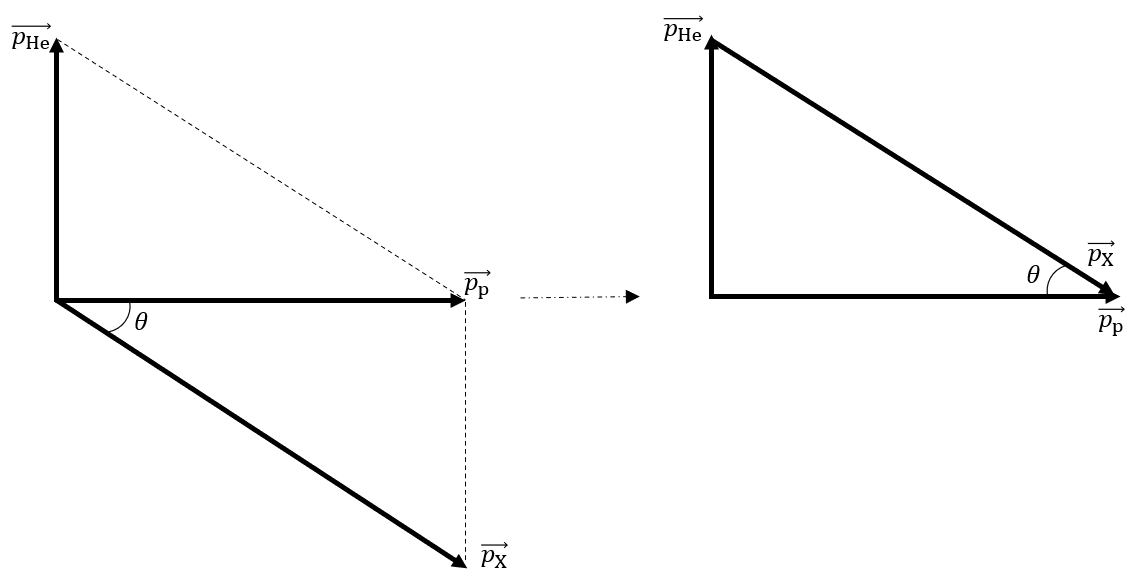
\includegraphics[scale=0.8]{../figs/VN12-2021-PH-TP037-3}
	\end{center}
	
	Áp dụng định lý Py-ta-go:
	$$p_{\ce{X}}^2 = p_{\ce{He}}^2 + p_{\ce{p}}^2$$
	
	Với $p^2=2mK$, ta được:
	$$2 m_{\ce{X}} K_{\ce{X}} = 2 m_{\ce{He}} K_{\ce{He}} +  2 m_{\ce{p}} K_{\ce{p}} $$
	
	Giải phương trình, tìm được:
	$$K_{\ce{X}} = \SI{3.57}{MeV}$$
		
	}
	
	\item \mkstar{2} [7]
	
	\cauhoi
	{Cho phản ứng hạt nhân sau:
		$$\ce{^9_4 Be} + \ce{p} \longrightarrow \ce{X} + \ce{^6_3 Li}$$
		
		Biết $m_{\ce{Be}} = \SI{9.01219}{u}$, $m_{\ce{p}} = \SI{1.00783}{u}$, $m_{\ce{X}} = \SI{4.00620}{u}$, $m_{\ce{Li}} = \SI{6.01515}{u}$, $\SI{1}{u} = \SI{931}{MeV/c^2}$. Cho hạt $\ce{p}$ có động năng $K_{\ce{p}} = \SI{5.45}{MeV}$ bắn phá hạt nhân $\ce{Be}$ đứng yên, hạt nhân $\ce{Li}$ bay ra với động năng $\SI{3.55}{MeV}$. Động năng của hạt $\ce{X}$ bay ra có giá trị là
		\begin{mcq}(4)
			\item $\SI{0.66}{MeV}$.
			\item $\SI{0.66}{eV}$.
			\item $\SI{66}{MeV}$.
			\item $\SI{660}{eV}$.
		\end{mcq}
	}
	
	\loigiai
	{		\textbf{Đáp án: A.}
		
		Năng lượng tỏa ra hoặc thu vào của phản ứng:
	$$Q=(m_\text{t} - m_\text{s})c^2 = \SI{-1.23823}{MeV}$$
	
	Lại có $Q=K_{\text{s}} - K_{\text{t}} = K_{\ce{X}} + K_{\ce{Li}} - K_{\ce{p}} \Rightarrow K_{\ce{X}} = \SI{0.66}{MeV}$
		
	}
	\item \mkstar{3} [1]
	
	\cauhoi
	{Người ta dùng hạt $\ce{\alpha}$ có động năng $K_{\ce{\alpha}}$ bắn vào hạt nhân nhôm $\ce{^27_13 Al}$ đứng yên gây ra phản ứng 
		$$\ce{^4_2 He} + \ce{^27_13 Al} \longrightarrow \ce{^30_15 P} + \ce{^1_0 n}$$
		Biết hạt nơtron và hạt nhân $\ce{^30_15 P}$ sinh ra sau phản ứng có động năng lần lượt là $\SI{1.8}{MeV}$ và $\SI{1}{MeV}$. Biết khối lượng của các hạt lần lượt là $m_{\ce{\alpha}} = \SI{4.00151}{u}$; $m_{\ce{Al}} = \SI{26.97435}{u}$; $m_{\ce{P}} = \SI{29.97005}{u}$; $m_{\ce{n}} = \SI{1.00867}{u}$. Động năng hạt $\ce{\alpha}$ là $K_{\ce{\alpha}}$ bằng
		\begin{mcq}(4)
			\item $\SI{5.464}{MeV}$.
			\item $\SI{4.232}{MeV}$.
			\item $\SI{5.644}{MeV}$.
			\item $\SI{4.328}{MeV}$.
		\end{mcq}
	}
	
	\loigiai
	{		\textbf{Đáp án: A.}
		
		Ta có năng lượng tỏa ra hoặc thu vào từ phản ứng là
	$$Q=(m_\text{t} - m_\text{s})c^2 = \SI{-2.66409}{MeV}$$
	
	Mà $Q=K_\text{s} - K_\text{t} \Rightarrow K_{\ce{P}} + K_{\ce{n}} - K_{\ce{\alpha}} - K_{\ce{Al}} = \SI{-2.66409}{MeV}$, suy ra $K_{\ce{\alpha}} = \SI{5.464}{MeV}$. (Chú ý rằng $K_{\ce{Al}}=0$ vì hạt nhân nhôm đứng yên)
	}
	\item \mkstar{3} [4]
	
	\cauhoi
	{Dùng một hạt $\ce{\alpha}$ có động năng $\SI{7.7}{MeV}$ bắn vào hạt nhân $\ce{^14_7 N}$ đang đứng yên gây ra phản ứng
		$$\ce{^4_2 He} + \ce{^14_7 N} \longrightarrow \ce{^1_1 p} + \ce{^17_8 O}$$
		Hạt proton bay ra theo phương vuông góc với phương bay tới của hạt $\ce{^4_2 He}$. Cho khối lượng các hạt nhân: $m_{\ce He} = \SI{4.0015}{u}$, $m_{\ce{N 14}} = \SI{13.9992}{u}$, $m_{\ce{O 17}} = \SI{16.9947}{u}$, $m_{\ce{p}} = \SI{1.0073}{u}$. Động năng của hạt nhân $\ce{^17_8 O}$ là
		\begin{mcq}(4)
			\item $\SI{2.075}{MeV}$.
			\item $\SI{2.214}{MeV}$.
			\item $\SI{6.145}{MeV}$.
			\item $\SI{1.345}{MeV}$.
		\end{mcq}
	}
	
	\loigiai
	{		\textbf{Đáp án: A.}
		
		
		Áp dụng định luật bảo toàn động lượng cho các hạt trước và sau phản ứng:
		$$\vec p_{\ce{\alpha}} = \vec p_{\ce{p}} + \vec p_{\ce{O}}$$
		
		Hình vẽ minh họa:
		\begin{center}
			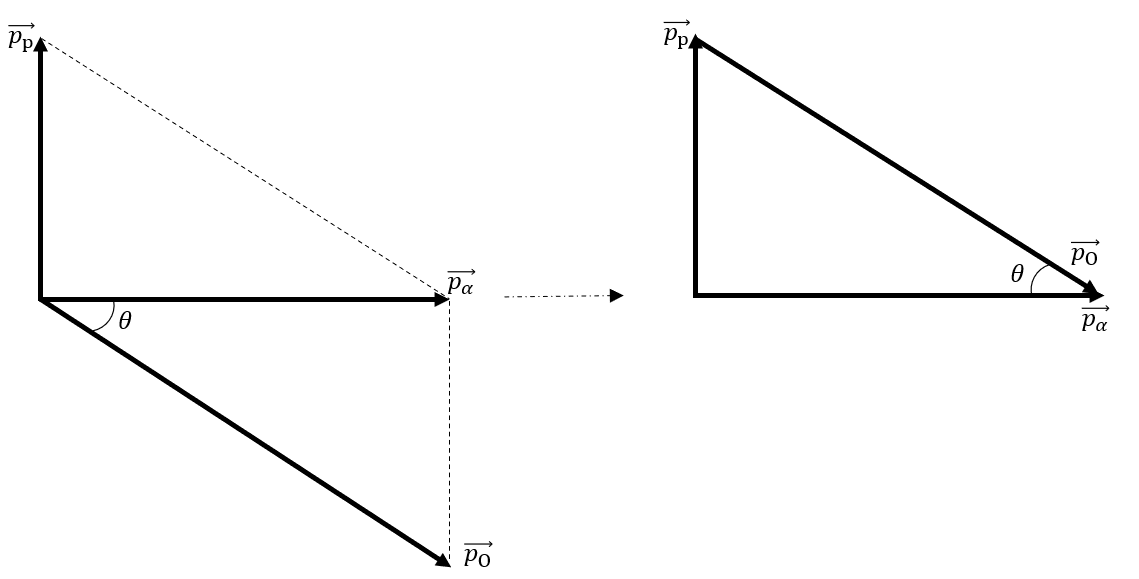
\includegraphics[scale=0.8]{../figs/VN12-2021-PH-TP037-2}
		\end{center}
		
		Áp dụng định lý Py-ta-go:
		$$p_{\ce{O}}^2 = p_{\ce{\alpha}}^2 + p_{\ce{p}}^2$$
		
		Với $p^2=2mK$, ta được:
		$$2 m_{\ce{O}} K_{\ce{O}} = 2 m_{\ce{\alpha}} K_{\ce{\alpha}} +  2 m_{\ce{p}} K_{\ce{p}} $$
		
		Kết hợp với công thức tính năng lượng tỏa ra hoặc thu vào:
		$$Q=(m_{\text{t}} - m_{\text{s}})c^2 = \SI{-1.21095}{MeV} = K_{\text s} - K_{\text t} = K_{\ce{p}} + K_{\ce{O}} - K_{\ce{He}}$$
		
		Giải hệ 2 phương trình, tìm được:
		$K_{\ce{p}} = \SI{4.417}{MeV}$ và $K_{\ce{O}} = \SI{2.072}{MeV}$
		
		Động năng của hạt nhân $\ce{^17_8 O}$ là xấp xỉ $\SI{2.075}{MeV}$.
	}
	\item \mkstar{3} [12]
	
	\cauhoi
	{Hạt nhân $\ce{^222_86 Rn}$ phóng xạ $\alpha$ tạo thành hạt nhân X. Ban đầu, hạt nhân $\ce{^222_86 Rn}$ đứng yên. Khối lượng mỗi hạt nhân bằng số khối của nó (đơn vị u). Ngay sau khi tạo thành, hạt $\ce{\alpha}$ và hạt X có tốc độ lần lượt là $v_1=\SI{2e7}{m/s}$ và $v_2$. Giá trị của $v_2$ xấp xỉ bằng
		\begin{mcq}(2)
			\item $\SI{366.972e3}{m/s}$.
			\item $\SI{10.034e5}{m/s}$.
			\item $\SI{109.021e3}{m/s}$.
			\item $\SI{605.015e3}{m/s}$.
		\end{mcq}
	}
	
	\loigiai
	{		\textbf{Đáp án: A.}
		
		Phản ứng hạt nhân:
	$$\ce{^222_86 Rn} \longrightarrow \ce{^4_2 He} + \ce{^218_84 X}$$
	
	Áp dụng định luật bảo toàn động lượng cho các hạt trước và sau phản ứng:
	$$\vec p_{\ce{Rn}} = \vec p_{\ce{\alpha}} + \vec p_{\ce{X}}$$
	
	Do $\vec p_{\ce{Rn}} = 0$ nên $\vec p_{\ce{\alpha}} + \vec p_{\ce{X}}$, suy ra:
	$$p_{\ce{\alpha}} = p_{\ce{X}}$$
	
	Với $p=\sqrt{2mK}$, và $\SI{1}{u} = \SI{1.6605e-27}{kg}$ ta được:
	$$2 m_{\ce{\alpha}} K_{\ce{\alpha}} = 2 m_{\ce{X}} K_{\ce{X}} \Rightarrow v_{\ce{X}} = \SI{366.972e3}{m/s}$$
	}
	\item \mkstar{4} [2]
	
	\cauhoi
	{Bắn một hạt proton có khối lượng $m_{\ce{H}}$ vào hạt nhân $\ce{^7_3 Li}$ đứng yên. Phản ứng tạo ra hai hạt nhân X giống nhau bay ra với vận tốc có cùng độ lớn và có phương vuông góc với nhau. Nếu xem gần đúng khối lượng hạt nhân theo đơn vị u bằng số khối của nó thì tỉ số tốc độ $v'$ của hạt X và $v$ của hạt proton là
		\begin{mcq}(4)
			\item $\dfrac{v'}{v} = \dfrac{1}{4}$.
			\item $\dfrac{v'}{v} = \dfrac{\sqrt{2}}{4}$.
			\item $\dfrac{v'}{v} = \dfrac{\sqrt 2}{8}$.
			\item $\dfrac{v'}{v} = \dfrac{1}{2}$.
		\end{mcq}
	}
	
	\loigiai
	{		\textbf{Đáp án: C.}
		
		Áp dụng định luật bảo toàn động lượng cho các hạt trước và sau phản ứng:
$$\vec p_{\text t} = \vec p_{\text s} \Rightarrow p_{\ce{p}}^2 = p_{\ce{X}}^2 + p_{\ce{X}}^2 = 2p_{\ce{X}}^2$$

Mà theo liên hệ $p^2=2mK$, suy ra:
$$2 m_{\ce{p}} K_{\ce{p}} = 2 \cdot 2 m_{\ce{X}} K_{\ce{X}} \Rightarrow m_{\ce{p}} K_{\ce{p}} = 2 m_{\ce{X}} K_{\ce{X}}$$

Thay $K=\dfrac{1}{2} mv^2$, ta được:
$$m_{\ce{p}} \cdot \dfrac{1}{2} m_{\ce{p}} v_{\ce{p}}^2 = 2 m_{\ce{X}} \cdot \dfrac{1}{2} m_{\ce{X}} v_{\ce{X}}^2 \Rightarrow \dfrac{v_{\ce{X}}^2}{v_{\ce{p}}^2} = \dfrac{m_{\ce{p}}^2}{2 m_{\ce{X}}^2} = \dfrac{1^2}{2 \cdot 4^2} = \dfrac{1}{32} \Rightarrow \dfrac{v'}{v} = \sqrt{\dfrac{1}{32}} = \dfrac{\sqrt 2}{8}$$
		
	}
	
	\item \mkstar{4} [3]
	
	\cauhoi
	{Bắn hạt nơtron có động năng $\SI{2}{MeV}$ vào hạt nhân $\ce{^6_3 Li}$ đứng yên gây ra phản ứng
		$$\ce{^1_0 n} + \ce{^6_3 Li} \longrightarrow \ce{X} + \ce{\alpha}.$$
		Hạt $\ce{\alpha}$ và hạt nhân $\ce{X}$ bay ra theo các hướng hợp với hướng tới của nơtron những góc tương ứng bằng $\theta = 15^\circ$ và $\varphi = 30^\circ$. Lấy tỉ số giữa các khối lượng hạt nhân bằng tỉ số giữa các số khối của chúng. Bỏ qua bức xạ gamma. Năng lượng của phản ứng hạt nhân \textbf{gần với giá trị nào nhất?}
		\begin{mcq}(4)
			\item Tỏa $\SI{1.52}{MeV}$.
			\item Thu $\SI{1.66}{MeV}$. 
			\item Thu $\SI{1.52}{MeV}$.
			\item Tỏa $\SI{1.66}{MeV}$.
		\end{mcq}
	}
	
	\loigiai
	{		\textbf{Đáp án: B.}
		
		Áp dụng định luật bảo toàn động lượng cho các hạt trước và sau phản ứng:
	$$\vec p_{\ce{n}} = \vec p_{\ce{X}} + \vec p_{\ce{\alpha}}$$
	
	Hình vẽ minh họa:
	\begin{center}
		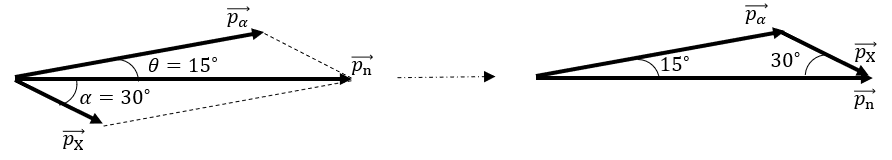
\includegraphics{../figs/VN12-2021-PH-TP037-1}
	\end{center}
	
	Áp dụng định lý hàm số sin:
	$$\dfrac{p_{\ce{n}}}{\sin 135^\circ} = \dfrac{p_{\ce{\alpha}}}{\sin 30^\circ} = \dfrac{p_{\ce{X}}}{\sin 15^\circ}$$
	
	Với $p=\sqrt{2mK}$, ta được:
	$$\dfrac{p_{\ce{n}}}{\sin 135^\circ} = \dfrac{p_{\ce{\alpha}}}{\sin 30^\circ} \Rightarrow \dfrac{\sqrt{2 m_{\ce{n}} K_{\ce{n}}}}{\sin 135^\circ} = \dfrac{\sqrt{2 m_{\ce{\alpha}} K_{\ce{\alpha}}}}{\sin 30^\circ}\Rightarrow K_{\ce{\alpha}} = \SI{0.25}{MeV} $$
	
	$$\dfrac{p_{\ce{n}}}{\sin 135^\circ} = \dfrac{p_{\ce{X}}}{\sin 15^\circ} \Rightarrow \dfrac{\sqrt{2 m_{\ce{n}} K_{\ce{n}}}}{\sin 135^\circ} = \dfrac{\sqrt{2 m_{\ce{X}} K_{\ce{X}}}}{\sin 15^\circ}\Rightarrow K_{\ce{X}} = \SI{0.09}{MeV} $$
	
	Năng lượng tỏa ra hoặc thu vào:
	$$Q=K_{\text{s}} - K_{\text{t}} = \SI{-1.66}{MeV}$$
	
	Do $Q<0$ nên phản ứng thu năng lượng.
	}
	
	
	
	
	
	
\end{enumerate}

\loigiai
{
	\begin{center}
		\textbf{BẢNG ĐÁP ÁN}
	\end{center}
	\begin{center}
		\begin{tabular}{|m{2.8em}|m{2.8em}|m{2.8em}|m{2.8em}|m{2.8em}|m{2.8em}|m{2.8em}|m{2.8em}|m{2.8em}|m{2.8em}|}
			\hline
			1.D  & 2.A  & 3.A  & 4.A  & 5.A  & 6.A  & 7.A & 8.C & 9.B & \\
			\hline
			
		\end{tabular}
	\end{center}
}

\whiteBGstarEnd
	\stopcontents[mychapters]
	
\setcounter{mychapter}{36}
	\mychapter{Phóng xạ}
	\startcontents[mychapters]
	\printcontents[mychapters]{}{0}{\setcounter{tocdepth}{1}}
	\whiteBGstarBegin
\setcounter{section}{0}
\section{Lý thuyết: Hiện tượng phóng xạ hạt nhân và các loại tia phóng xạ}
\begin{enumerate}[label=\bfseries Câu \arabic*:]
	\item \mkstar{1} [1]
	
	\cauhoi
	{Phóng xạ hạt nhân là phản ứng ...
		\begin{mcq}(2)
			\item nhiệt hạch.
			\item hạt nhân thu năng lượng.
			\item phân hạch.
			\item hạt nhân tỏa năng lượng.
		\end{mcq}
	}
	
	\loigiai
	{		\textbf{Đáp án: D.}
		
		Phóng xạ hạt nhân là phản ứng hạt nhân tỏa năng lượng.
		
	}
	
	\item \mkstar{1} [1]
	
	\cauhoi
	{Phản ứng hạt nhân nào sau đây là quá trình phóng xạ?
		\begin{mcq}(2)
			\item $\ce{^210_84 Po} \longrightarrow \ce{^4_2 He} + \ce{^206_82 Pb}$.
			\item $\ce{^1_0 n} + \ce{^235_92 U} \longrightarrow \ce{^139_54 Xe} + \ce{^95_38 Sr} + 2 \ce{^1_0 n}$.
			\item $\ce{^7_3 Li} + \ce{^2_1 H} \longrightarrow 2 \ce{^4_2 He} + \ce{^1_0 n}$.
			\item $\ce{^4_2 He} + \ce{^27_13 Al} \longrightarrow \ce{^1_0 n} + \ce{^30_15 P}$.
		\end{mcq}
	}
	
	\loigiai
	{		\textbf{Đáp án: A.}
		
		Phản ứng
		$$\ce{^210_84 Po} \longrightarrow \ce{^4_2 He} + \ce{^206_82 Pb}$$
		là quá trình phóng xạ.
		
		Các phản ứng còn lại là phản ứng nhiệt hạch, phân hạch hoặc phản ứng hạt nhân thông thường.
		
	}
		\item \mkstar{1} [3]
	
	\cauhoi
	{Chọn phát biểu đúng về tia phóng xạ $\alpha$.
		\begin{mcq}
			\item Không bị lệch khi đi qua điện trường và từ trường.
			\item Có vận tốc bằng vận tốc ánh sáng trong chân không.
			\item Là dòng các hạt nhân $\ce{^4_2 He}$.
			\item Có khả năng đâm xuyên mạnh hơn tia phóng xạ $\gamma$.
		\end{mcq}
	}
	
	\loigiai
	{		\textbf{Đáp án: C.}
		
		Tia phóng xạ $\alpha$ là dòng các hạt nhân $\ce{^4_2 He}$, có bị lệch trong điện trường và từ trường, khả năng đâm xuyên yếu hơn và vận tốc nhỏ hơn nhiều so với tia $\gamma$.
		
	}
	
	\item \mkstar{1} [3]
	
	\cauhoi
	{Tia nào sau đây \textbf{không} phải là tia phóng xạ?
		\begin{mcq}(4)
			\item Tia $\alpha$.
			\item Tia $\beta^+$.
			\item Tia $\gamma$.
			\item Tia X.
		\end{mcq}
	}
	
	\loigiai
	{		\textbf{Đáp án: D.}
		
		Tia X bản chất là sóng điện từ, không phải tia phóng xạ.
		
	}
	\item \mkstar{1} [12]
	
	\cauhoi
	{Cặp tia nào dưới đây có cùng bản chất là sóng điện từ?
		\begin{mcq}(2)
			\item Tia $\beta ^+$ và tia $\alpha$.
			\item Tia hồng ngoại và tia tử ngoại.
			\item Tia $\alpha$ và tia tử ngoại.
			\item Tia $\beta ^+$ và tia $\beta ^-$.
		\end{mcq}
	}
	
	\loigiai
	{		\textbf{Đáp án: B.}
		
		Tia hồng ngoại và tia tử ngoại đều có bản chất là sóng điện từ.
		
	}
	\item \mkstar{1} [5]

\cauhoi
{Hạt nhân $\ce{^A_Z X}$ phóng xạ $\alpha$ tạo ra hạt nhân $\ce{Y}$. Phương trình phản ứng có dạng:
	\begin{mcq}(2)
		\item $\ce{^A_Z X} \longrightarrow \alpha + \ce{^{A-4}_{Z-2} Y}$.
		\item $\ce{^A_Z X} \longrightarrow \alpha + \ce{^{A-2}_{Z-4} Y}$.
		\item $\ce{^A_Z X} \longrightarrow \alpha + \ce{^{A-2}_{Z-2} Y}$.
		\item $\ce{^A_Z X} \longrightarrow \alpha + \ce{^{A-4}_{Z-4} Y}$.
	\end{mcq}
}

\loigiai
{		\textbf{Đáp án: A.}
	
	Áp dụng định luật bảo toàn số khối và bảo toàn điện tích thì phản ứng đúng là
	$$\ce{^A_Z X} \longrightarrow \alpha + \ce{^{A-4}_{Z-2} Y}$$
	
}
\item \mkstar{1} [5]

\cauhoi
{Hạt nhân $\ce{^A_Z X}$ phóng xạ $\beta^-$ tạo ra hạt nhân $\ce{Y}$. Phương trình phản ứng có dạng:
	\begin{mcq}(2)
		\item $\ce{^A_Z X} \longrightarrow \beta^- + \ce{^{A}_{Z-1} Y}$.
		\item $\ce{^A_Z X} \longrightarrow \beta^- + \ce{^{A-1}_{Z} Y}$.
		\item $\ce{^A_Z X} \longrightarrow \beta^- + \ce{^{A+1}_{Z} Y}$.
		\item $\ce{^A_Z X} \longrightarrow \beta^- + \ce{^{A}_{Z+1} Y}$.
	\end{mcq}
}

\loigiai
{		\textbf{Đáp án: D.}
	
	Áp dụng định luật bảo toàn số khối và bảo toàn điện tích thì phản ứng đúng là
	$$\ce{^A_Z X} \longrightarrow \beta^- + \ce{^{A}_{Z+1} Y}$$
	
}
	\item \mkstar{2} [1]
	
	\cauhoi
	{Đồng vị $\ce{^30_15 P}$ biến thành hạt nhân $\ce{^30_14 Si}$ sau khi phóng xạ tia
		\begin{mcq}(4)
			\item $\beta^-$. 
			\item $\gamma$. 
			\item $\beta^+$. 
			\item $\alpha$. 
		\end{mcq}
	}
	
	\loigiai
	{		\textbf{Đáp án: C.}
		
		Phương trình phản ứng:
		$$\ce{^30_15 P} \longrightarrow \ce{^30_14 Si} + \ce{^A_Z X}$$
		
		Áp dụng định luật bảo toàn số khối và bảo toàn điện tích, tìm được X là hạt $\beta^+$ ($\ce{^0_1 e}$).
		
	}
	

	\item \mkstar{2} [13]

\cauhoi
{Hạt nhân $\ce{^226_88 Ra}$ phóng xạ ra 3 hạt $\alpha$ và một hạt $\beta^-$ trong chuỗi phóng xạ liên tiếp. Khi đó hạt nhân tạo thành là
	\begin{mcq}(4)
		\item $\ce{^214_82 X}$.
		\item $\ce{^212_83 X}$.
		\item $\ce{^214_83 X}$.
		\item $\ce{^212_82 X}$.
	\end{mcq}
}

\loigiai
{		\textbf{Đáp án: C.}
	
	Phương trình phản ứng:
	$$\ce{^226_88 Ra}\ \ldots \longrightarrow \ldots\ 3 \ce{^4_2 He} + \ce{^0_{-1} e} + \ce{X}$$
	
	Áp dụng định luật bảo toàn số khối và bảo toàn điện tích, tìm được $X$ là $\ce{^214_83 X}$.
	
}
	\item \mkstar{2} [5]

\cauhoi
{Khi một hạt nhân nguyên tử phóng xạ lần lượt một tia $\alpha$ rồi một tia $\beta^+$ thì hạt nhân nguyên tử sẽ biến đổi như thế nào?
	\begin{mcq}
		\item Số khối giảm 4, số neutron giảm 1.
		\item Số neutron giảm 3, số proton giảm 1.
		\item Số proton giảm 1, số neutron tăng 3.
		\item Số khối giảm 4, số proton tăng 1.
	\end{mcq}
}

\loigiai
{		\textbf{Đáp án: A.}
	
	Phương trình phản ứng:
	$$\ce{^A_Z X}\ \ldots \longrightarrow \ldots\ \ce{^4_2 He} + \ce{^0_1 e} + Y$$
	
	Áp dụng định luật bảo toàn số khối và bảo toàn điện tích, tìm được Y là $\ce{^{A-4}_{Z-3} Y}$.
	
	Vậy số khối giảm 4, số proton giảm 3, dẫn đến số neutron giảm 1.
	
}

\end{enumerate}

\loigiai
{
	\begin{center}
		\textbf{BẢNG ĐÁP ÁN}
	\end{center}
	\begin{center}
		\begin{tabular}{|m{2.8em}|m{2.8em}|m{2.8em}|m{2.8em}|m{2.8em}|m{2.8em}|m{2.8em}|m{2.8em}|m{2.8em}|m{2.8em}|}
			\hline
			1.D  & 2.A  & 3.C  & 4.D  & 5.B  & 6.A  & 7.D & 8.C & 9.C & 10.A \\
			\hline
			
		\end{tabular}
	\end{center}
}

\section{Dạng bài: Định luật phóng xạ}
\begin{enumerate}[label=\bfseries Câu \arabic*:]
		\item \mkstar{1} [1]
	
	\cauhoi
	{Một chất phóng xạ có chu kì bán rã $T=\SI{8}{h}$, hằng số phân rã của chất phóng xạ này bằng
		\begin{mcq}(4)
			\item $\SI{1.2e-5}{s^{-1}}$.
			\item $\SI{2.4e-5}{s^{-1}}$.
			\item $\SI{2.6e-5}{s^{-1}}$.
			\item $\SI{1.3e-5}{s^{-1}}$.
		\end{mcq}
	}
	
	\loigiai
	{		\textbf{Đáp án: B.}
		
		Hằng số phân rã:
		$$\lambda = \dfrac{\ln 2}{T} = \dfrac{\ln 2}{\SI{28800}{s}} = \SI{2.4e-5}{s^{-1}}$$
		
	}
	\item \mkstar{1} [5]
	
	\cauhoi
	{Hằng số phóng xạ của Rubidi là $\SI{0.00077}{s^{-1}}$. Chu kì bán rã của nó tính theo đơn vị phút nhận giá trị nào sau đây?
		\begin{mcq}(4)
			\item 150 phút.
			\item 15 phút.
			\item 900 phút.
			\item 600 phút.
		\end{mcq}
	}
	
	\loigiai
	{		\textbf{Đáp án: B.}
		
		Hằng số phóng xạ được tính theo công thức:
		$$\lambda = \dfrac{\ln 2}{T} \Rightarrow T = \SI{900}{s}$$
		
		Vậy $T=15$ phút.
		
	}

		\item \mkstar{2} [13]
	
	\cauhoi
	{Ban đầu có $\SI{4e20}{}$ hạt nhân $\ce{^60_27 Co}$ với chu kì bán rã là $T=\SI{5.3}{}$ năm. Số hạt nhân $\ce{^60_27 Co}$ còn lại sau 10,6 năm bằng
		\begin{mcq}(4)
			\item $\SI{0.5e20}{}$.
			\item $\SI{2e20}{}$.
			\item $\SI{1e20}{}$.
			\item $\SI{0.2e20}{}$.
		\end{mcq}
	}
	
	\loigiai
	{		\textbf{Đáp án: C.}
		
		Số hạt nhân còn lại:
		$$N=N_0 2^{-\frac{t}{T}} = \SI{1e20}{}$$
		
	}
	\item \mkstar{2} [13]
	
	\cauhoi
	{Chất phóng xạ iốt $\ce{^131_53 I}$ có chu kì bán rã là $T=8$ ngày đêm. Ban đầu có $\SI{16e19}{}$ hạt nhân chất này. Sau 24 ngày đêm, số hạt nhân $\ce{^131_53 I}$ bị phân rã bằng
		\begin{mcq}(4)
			\item $\SI{4.8e20}{}$.
			\item $\SI{2e19}{}$.
			\item $\SI{5.3e19}{}$.
			\item $\SI{1.4e20}{}$.
		\end{mcq}
	}
	
	\loigiai
	{		\textbf{Đáp án: D.}
		
		Số hạt nhân bị phân rã:
		$$\Delta N = N_0 (1-2^{-\frac{t}{T}}) = \SI{1.4e20}{}$$
		
	}
\item \mkstar{2} [5]

\cauhoi
{Một lượng chất phóng xạ có khối lượng ban đầu $m_0$. Sau 4 chu kì bán rã khối lượng chất phóng xạ còn lại là
	\begin{mcq}(4)
		\item $\dfrac{m_0}{5}$.
		\item $\dfrac{m_0}{25}$.
		\item $\dfrac{m_0}{16}$.
		\item $\dfrac{m_0}{50}$.
	\end{mcq}
}

\loigiai
{		\textbf{Đáp án: C.}
	
	Sau 4 chu kì bán rã $(t=4T)$ thì khối lượng chất phóng xạ còn lại là:
	$$m=m_0 2^{-\frac{t}{T}} = m_0 \cdot \dfrac{1}{16}$$
	
	Vậy $m=\dfrac{m_0}{16}$.
	
}
	\item \mkstar{3} [1]
	
	\cauhoi
	{Hạt nhân Pôlôni $(\ce{^210_84 Po})$ phóng ra hạt $\alpha$ và biến thành hạt nhân Chì $(\ce{Pb})$ bền, có chu kì bán rã là 138 ngày. Ban đầu có một mẫu Pôlôni nguyên chất có khối lượng $\SI{30}{g}$. Cho số A-vô-ga-đrô $N_\text{A} = \SI{6.02e23}{mol^{-1}}$. Sau 414 ngày số hạt nhân Chì hình thành bằng
		\begin{mcq}(4)
			\item $\SI{7.671e22}{}$.
			\item $\SI{7.525e23}{}$.
			\item $\SI{7.671e23}{}$.
			\item $\SI{7.525e22}{}$.
		\end{mcq}
	}
	
	\loigiai
	{		\textbf{Đáp án: D.}
		
		Số hạt Pôlôni ban đầu:
		$$N_0 = \dfrac{m}{M} N_\text{A} = \SI{8.6e22}{}$$
		
		Số hạt Chì tạo thành cũng đồng thời là số hạt Pôlôni bị phân rã:
		$$\Delta N=N_0 (1-2 ^{-\frac{t}{T}} )= \SI{7.525e22}{}$$
		
	}
	
	\item \mkstar{3} [1]
	
	\cauhoi
	{I-ốt $(\ce{^131_53 I})$ là chất phóng xạ $\beta^-$ với chu kì bán rã 8 ngày. Ban đầu có $\SI{200}{g}$ I-ốt $(\ce{^131_53 I})$. Khối lượng I-ốt trên bị phân rã trong ngày thứ 10 kể từ thời điểm ban đầu là
		\begin{mcq}(4)
			\item $\SI{115.9}{g}$.
			\item $\SI{8.39}{g}$.
			\item $\SI{7.61}{g}$.
			\item $\SI{84}{g}$.
		\end{mcq}
	}
	
	\loigiai
	{		\textbf{Đáp án: C.}
		
		Khối lượng I-ốt trên bị phân rã trong ngày thứ 10 là hiệu giữa khối lượng bị phân rã cuối ngày 10 với cuối ngày 9 kể từ thời điểm ban đầu.
		
		Khối lượng I-ốt bị phân rã cuối ngày 10:
		$$\Delta N_1 = N_0 (1-2^{-\frac{t_1}{T}}) = \SI{115.9}{g}$$
		
		Khối lượng I-ốt bị phân rã cuối ngày 9:
		$$\Delta N_2 = N_0 (1-2^{-\frac{t_2}{T}}) = \SI{108.3}{g}$$
		
		Vậy khối lượng I-ốt trên bị phân rã trong ngày thứ 10 là $\Delta N_1 - \Delta N_2 = \SI{7.6}{g}$.
		
	}
	
	\item \mkstar{3} [3]
	
	\cauhoi
	{Chất phóng xạ $\ce{X}$ có chu kì bán rã là $\SI{8.5}{s}$. Ban đầu có một mẫu $\ce{X}$ nguyên chất. Sau bao lâu thì số hạt nhân $\ce{X}$ bị phân rã bằng 15 lần số hạt nhân $\ce{X}$ còn lại trong mẫu?
		\begin{mcq}(4)
			\item $\SI{38.0}{s}$.
			\item $\SI{8.5}{s}$.
			\item $\SI{34.0}{s}$.
			\item $\SI{25.5}{s}$.
		\end{mcq}
	}
	
	\loigiai
	{		\textbf{Đáp án: C.}
		
		Số hạt bị phân rã bằng 15 lần số hạt còn lại:
		$$\dfrac{\Delta N}{N} = 15 \Rightarrow \dfrac{1-2^{-\frac{t}{T}}}{2^{-\frac{t}{T}}} = 15 \Rightarrow t = \SI{34.0}{s}$$
		
	}
	\item \mkstar{3} [13]
	
	\cauhoi
	{
		Chất phóng xạ X có số hạt nhân giảm dần theo thời gian như đồ thị. Chu kì bán rã của chất phóng xạ X bằng
		\begin{mcq}(2)
			\item 16 ngày đêm.
			\item 10 ngày đêm.
			\item 6 ngày đêm.
			\item 8 ngày đêm.
		\end{mcq}
		\begin{center}
			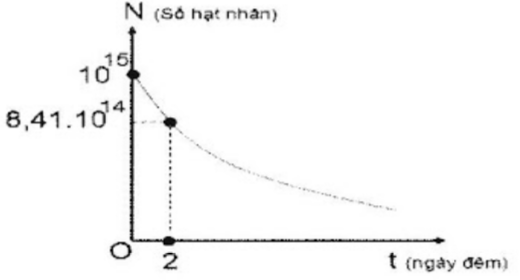
\includegraphics[scale=0.8]{../figs/VN12-2021-PH-TP038-1}
		\end{center}
		
	}
	
	\loigiai
	{		\textbf{Đáp án: D.}
		
		Tại thời điểm $t=0$ thì $N_0 = \SI{e15}{}$.
		
		Tại thời điểm $t=2$ thì $N=\SI{8.41e14}{}$.
		
		Áp dụng công thức:
		$$N=N_0 2^{-\frac{t}{T}} \Rightarrow T = 8$$
		
	}
	\item \mkstar{4} [10]
	
	\cauhoi
	{Ban đầu $(t=0)$ có một mẫu chất phóng xạ X nguyên chất. Ở thời điểm $t$ số hạt nhân X chưa bị phân rã bằng $20\%$ số hạt nhân ban đầu. Đến thời điểm $t+100\ \text{s}$ số hạt nhân X chưa bị phân rã bằng $5\%$ số hạt nhân ban đầu. Chu kì bán rã của chất phóng xạ đó là
		\begin{mcq}(4)
			\item 50 s.
			\item 25 s.
			\item 400 s. 
			\item 200 s.
		\end{mcq}
	}
	
	\loigiai
	{		\textbf{Đáp án: A.}
		
		Ở thời điểm $t$ số hạt nhân X chưa bị phân rã bằng $20\%$ số hạt nhân ban đầu:
		
		$$\dfrac{N}{N_0}=\dfrac{1}{5} \Rightarrow 2^{-\frac{t}{T}} = \dfrac{1}{5}$$
		
		Đến thời điểm $t+100\ \text{s}$ số hạt nhân X chưa bị phân rã bằng $5\%$ số hạt nhân ban đầu:
		
		$$\dfrac{N}{N_0}=\dfrac{1}{20} \Rightarrow 2^{-\frac{(t+100)}{T}} = \dfrac{1}{20} \Rightarrow 2^{-\frac{t}{T}} \cdot 2^{-\frac{-100}{T}} = \dfrac{1}{20} \Rightarrow T = \SI{50}{s}$$
	}


\item \mkstar{4} [13]

\cauhoi
{Ban đầu có $N_0$ hạt nhân của chất phóng xạ X có chu kì bán rã là $T$, gọi $\Delta t$ là khoảng thời gian mà số hạt nhân còn lại của một lượng chất phóng xạ giảm đi $e$ lần so với ban đầu (với $\ln e = 1$). Nếu sau khoảng thời gian $\SI{0.5}{} \Delta t$ số hạt nhân chất phóng xạ X còn lại bằng bao nhiêu phần trăm so với lúc ban đầu?
	\begin{mcq}(4)
		\item $\SI{70.71}{\percent}$. 
		\item $\SI{50.00}{\percent}$.
		\item $\SI{60.65}{\percent}$.
		\item $\SI{82.44}{\percent}$.
	\end{mcq}
}

\loigiai
{		\textbf{Đáp án: C.}
	
	Dựa vào công thức $N=N_0 e^{-\lambda \Delta t}$, để $N$ giảm đi $e$ lần so với ban đầu thì $\dfrac{N}{N_0} = \dfrac{1}{e} = e^{-1}$. Do đó:
	$$-\lambda \Delta t = -1 \Rightarrow \Delta t = \dfrac{1}{\lambda}$$
	
	Sau khoảng thời gian $\SI{0.5}{} \Delta t$ thì số hạt còn lại là
	$$\dfrac{N}{N_0} = e^{-\lambda \cdot \frac{1}{2\lambda}} = \SI{60.65}{\percent}$$
	
}


\end{enumerate}

\loigiai
{
	\begin{center}
		\textbf{BẢNG ĐÁP ÁN}
	\end{center}
	\begin{center}
		\begin{tabular}{|m{2.8em}|m{2.8em}|m{2.8em}|m{2.8em}|m{2.8em}|m{2.8em}|m{2.8em}|m{2.8em}|m{2.8em}|m{2.8em}|}
			\hline
			1.B  & 2.B  & 3.C  & 4.D  & 5.C  & 6.D  & 7.C & 8.C & 9.D & 10.A \\
			\hline
			11.C  & & & & & & & & &  \\
			\hline
			
		\end{tabular}
	\end{center}
}


\whiteBGstarEnd
	\stopcontents[mychapters]
	
%\setcounter{mychapter}{37}
%	\mychapter{Phản ứng phân hạch - Phản ứng nhiệt hạch}
%	\startcontents[mychapters]
%	\printcontents[mychapters]{}{0}{\setcounter{tocdepth}{1}}
%	\whiteBGstarBegin
\setcounter{section}{0}
\section{Lý thuyết: }
\begin{enumerate}[label=\bfseries Câu \arabic*:]
	\item \mkstar{1} [2]
	
	\cauhoi
	{ABC?
		\begin{mcq}(2)
			\item ABC. 
			\item ABC. 
			\item ABC. 
			\item ABC. 
		\end{mcq}
	}
	
	\loigiai
	{		\textbf{Đáp án: ABC.}
		
		ABC.
		
	}
	
	\item \mkstar{1} [2]
	
	\cauhoi
	{ABC?
		\begin{mcq}(4)
			\item ABC. 
			\item ABC. 
			\item ABC. 
			\item ABC. 
		\end{mcq}
	}
	
	\loigiai
	{		\textbf{Đáp án: ABC.}
		
		ABC.
		
	}
	
	\item \mkstar{1} [2]
	
	\cauhoi
	{ABC?
		\begin{mcq}
			\item ABC. 
			\item ABC. 
			\item ABC. 
			\item ABC. 
		\end{mcq}
	}
	
	\loigiai
	{		\textbf{Đáp án: ABC.}
		
		ABC.
		
	}
	
	\item \mkstar{1} [2]
	
	\cauhoi
	{ABC?
		\begin{mcq}
			\item ABC. 
			\item ABC. 
			\item ABC. 
			\item ABC. 
		\end{mcq}
	}
	
	\loigiai
	{		\textbf{Đáp án: ABC.}
		
		ABC.
		
	}
	
	\item \mkstar{1} [2]
	
	\cauhoi
	{ABC?
		\begin{mcq}
			\item ABC. 
			\item ABC. 
			\item ABC. 
			\item ABC. 
		\end{mcq}
	}
	
	\loigiai
	{		\textbf{Đáp án: ABC.}
		
		ABC.
		
	}
	
\end{enumerate}

\loigiai
{
	\begin{center}
		\textbf{BẢNG ĐÁP ÁN}
	\end{center}
	\begin{center}
		\begin{tabular}{|m{2.8em}|m{2.8em}|m{2.8em}|m{2.8em}|m{2.8em}|m{2.8em}|m{2.8em}|m{2.8em}|m{2.8em}|m{2.8em}|}
			\hline
			1.D  & 2.B  & 3.B  & 4.C  & 5.D  & 6.A  & 7.A & 8.A & 9.A & 10.A \\
			\hline
			
		\end{tabular}
	\end{center}
}

\section{Lý thuyết: }
\begin{enumerate}[label=\bfseries Câu \arabic*:]
	\item \mkstar{1} [2]
	
	\cauhoi
	{ABC?
		\begin{mcq}
			\item ABC. 
			\item ABC. 
			\item ABC. 
			\item ABC. 
		\end{mcq}
	}
	
	\loigiai
	{		\textbf{Đáp án: ABC.}
		
		ABC.
		
	}
	
	\item \mkstar{1} [2]
	
	\cauhoi
	{ABC?
		\begin{mcq}
			\item ABC. 
			\item ABC. 
			\item ABC. 
			\item ABC. 
		\end{mcq}
	}
	
	\loigiai
	{		\textbf{Đáp án: ABC.}
		
		ABC.
		
	}
	
	\item \mkstar{1} [2]
	
	\cauhoi
	{ABC?
		\begin{mcq}
			\item ABC. 
			\item ABC. 
			\item ABC. 
			\item ABC. 
		\end{mcq}
	}
	
	\loigiai
	{		\textbf{Đáp án: ABC.}
		
		ABC.
		
	}
	
	\item \mkstar{1} [2]
	
	\cauhoi
	{ABC?
		\begin{mcq}
			\item ABC. 
			\item ABC. 
			\item ABC. 
			\item ABC. 
		\end{mcq}
	}
	
	\loigiai
	{		\textbf{Đáp án: ABC.}
		
		ABC.
		
	}
	
	\item \mkstar{1} [2]
	
	\cauhoi
	{ABC?
		\begin{mcq}
			\item ABC. 
			\item ABC. 
			\item ABC. 
			\item ABC. 
		\end{mcq}
	}
	
	\loigiai
	{		\textbf{Đáp án: ABC.}
		
		ABC.
		
	}
	
\end{enumerate}

\loigiai
{
	\begin{center}
		\textbf{BẢNG ĐÁP ÁN}
	\end{center}
	\begin{center}
		\begin{tabular}{|m{2.8em}|m{2.8em}|m{2.8em}|m{2.8em}|m{2.8em}|m{2.8em}|m{2.8em}|m{2.8em}|m{2.8em}|m{2.8em}|}
			\hline
			1.D  & 2.B  & 3.B  & 4.C  & 5.D  & 6.A  & 7.A & 8.A & 9.A & 10.A \\
			\hline
			
		\end{tabular}
	\end{center}
}

\section{Lý thuyết: }
\begin{enumerate}[label=\bfseries Câu \arabic*:]
	\item \mkstar{1} [2]
	
	\cauhoi
	{ABC?
		\begin{mcq}
			\item ABC. 
			\item ABC. 
			\item ABC. 
			\item ABC. 
		\end{mcq}
	}
	
	\loigiai
	{		\textbf{Đáp án: ABC.}
		
		ABC.
		
	}
	
	\item \mkstar{1} [2]
	
	\cauhoi
	{ABC?
		\begin{mcq}
			\item ABC. 
			\item ABC. 
			\item ABC. 
			\item ABC. 
		\end{mcq}
	}
	
	\loigiai
	{		\textbf{Đáp án: ABC.}
		
		ABC.
		
	}
	
	\item \mkstar{1} [2]
	
	\cauhoi
	{ABC?
		\begin{mcq}
			\item ABC. 
			\item ABC. 
			\item ABC. 
			\item ABC. 
		\end{mcq}
	}
	
	\loigiai
	{		\textbf{Đáp án: ABC.}
		
		ABC.
		
	}
	
	\item \mkstar{1} [2]
	
	\cauhoi
	{ABC?
		\begin{mcq}
			\item ABC. 
			\item ABC. 
			\item ABC. 
			\item ABC. 
		\end{mcq}
	}
	
	\loigiai
	{		\textbf{Đáp án: ABC.}
		
		ABC.
		
	}
	
	\item \mkstar{1} [2]
	
	\cauhoi
	{ABC?
		\begin{mcq}
			\item ABC. 
			\item ABC. 
			\item ABC. 
			\item ABC. 
		\end{mcq}
	}
	
	\loigiai
	{		\textbf{Đáp án: ABC.}
		
		ABC.
		
	}
	
\end{enumerate}

\loigiai
{
	\begin{center}
		\textbf{BẢNG ĐÁP ÁN}
	\end{center}
	\begin{center}
		\begin{tabular}{|m{2.8em}|m{2.8em}|m{2.8em}|m{2.8em}|m{2.8em}|m{2.8em}|m{2.8em}|m{2.8em}|m{2.8em}|m{2.8em}|}
			\hline
			1.D  & 2.B  & 3.B  & 4.C  & 5.D  & 6.A  & 7.A & 8.A & 9.A & 10.A \\
			\hline
			
		\end{tabular}
	\end{center}
}

\whiteBGstarEnd
%	\stopcontents[mychapters]
	
\chapter[\textbf{Ôn tập: Chương VII. Hạt nhân nguyên tử}]{Ôn tập: Chương VII. Hạt nhân nguyên tử}
	\startcontents[chapters]
	\printcontents[chapters]{}{0}{\setcounter{tocdepth}{1}}
	\whiteBGstarBegin
\setcounter{section}{0}
\section{Tính chất và cấu tạo hạt nhân}
\begin{enumerate}[label=\bfseries Câu \arabic*:]
	\item \mkstar{1} [Trích đề thi năm 2007]
	
	\cauhoi
	{Hạt nhân Triti ($\ce{^3_1 T}$) có
			\begin{mcq}(2)
				\item 3 nuclôn, trong đó có 1 prôtôn.	
				\item 3 nơtrôn và 1 prôtôn.	
				\item 3 nuclôn, trong dó có 1 nơtrôn.	
				\item 3 prôtôn và 1 nơtrôn.
			\end{mcq}
	}
	
	\loigiai
	{		\textbf{Đáp án: A.}
		
		Hạt nhân Triti ($\ce{^3_1 T}$) có 3 nuclôn, trong đó có 1 prôtôn.
		
	}
	
	\item \mkstar{1} [Trích đề thi năm 2010]
	
	\cauhoi
	{So với hạt nhân $\ce{^{29}_{14} Si}$, hạt nhân $\ce{^{40}_{20} Ca}$ có nhiều hơn
		\begin{mcq}(2)
			\item 11 nơtrôn và 6 prôtôn.	
			\item 5 nơtrôn và 6 prôtôn.	
			\item 6 nơtrôn và 5 prôtôn.	
			\item 5 nơtrôn và l2 prôtôn.
		\end{mcq}
	}
	
	\loigiai
	{		\textbf{Đáp án: B.}
		
		Hạt nhân $\ce{^{29}_{14} Si}$ có $Z=14$ proton, $N=29-14=15$ nơtron.
		
		Hạt nhân $\ce{^{40}_{20} Ca}$ có $Z=20$ proton, $N=40-20=20$ nơtron.
		
		Vậy $\ce{^{40}_{20} Ca}$ có nhiều hơn 6 proton và 5 nơtron so với $\ce{^{29}_{14} Si}$ 
		
	}
	
	\item \mkstar{1} [Trích đề thi năm 2007]
	
	\cauhoi
	{Phát biểu nào là \textbf{sai}?
		\begin{mcq}
			\item Các đồng vị phóng xạ đều không bền.	
			\item Các nguyên tử mà hạt nhân có cùng số prôtôn nhưng có số nơtrôn khác nhau gọi là đồng vị.	
			\item Các đồng vị của cùng một nguyên tố có số nơtrôn khác nhau nên tính chất hóa học khác nhau.
			\item Các đồng vị của cùng một nguyên tố có cùng vị trí trong bảng hệ thống tuần hoàn. 
		\end{mcq}
	}
	
	\loigiai
	{		\textbf{Đáp án: C.}
		
		Các đồng vị của cùng một nguyên tố có tính chất hóa học giống nhau.
		
	}
		
\item \mkstar{1} [Trích đề thi năm 2011]

\cauhoi
{Theo thuyết tương đối, một êlectron có động năng bằng một nửa năng lượng nghỉ của nó thì êlectron này chuyển động với tốc độ bằng
	\begin{mcq} (4)
		\item $\text{2,24}\cdot 10^8\ \text{m/s}$.	
		\item $\text{2,75}\cdot 10^8\ \text{m/s}$.	
		\item $\text{1,67}\cdot 10^8\ \text{m/s}$.	
		\item $\text{2,59}\cdot 10^8\ \text{m/s}$.
	\end{mcq}
}

\loigiai
{		\textbf{Đáp án: A.}
	
	Động năng của hạt theo thuyết tương đối:
	$$W_\text{đ} =\dfrac{m_0c^2}{2}=E-E_0=  m_0 \left(\dfrac{1}{1-\sqrt{\dfrac{v^2}{c^2}}}-1\right)c^2 \Rightarrow v= \SI{2.24e8}{m/s}$$
	
}
\item \mkstar{2}

\cauhoi
{Cho biết khối lượng hạt nhân $\ce{^{234}_{92} U}$ là 233,9904 u. Biết khối lượng của hạt prôtôn và nơtrôn lần lượt là $m_{\ce{p}}= \text{1,007276}\ \text{u}$ và $m_{\ce{n}}= \text{l,008665}\ \text{u}$. Độ hụt khối của hạt nhân $\ce{^{234}_{92} U}$ bằng
	\begin{mcq}(4)
		\item 1,909422 u.	
		\item 3,460 u.	
		\item 0.	
		\item 2,056 u.
	\end{mcq}
}

\loigiai
{		\textbf{Đáp án: A.}
	
	Độ hụt khối:
	$$\Delta m = Zm_{\ce{p}} + (A-Z) m_{\ce{n}} - m_{\ce{X}} = \SI{1.909442}{u}$$
	
}
	\item \mkstar{2}
	
	\cauhoi
	{Urani tự nhiên gồm 3 đồng vị chính là $\ce{^{238} U}$ có khối lượng nguyên tử 238,0508 u (chiếm $\text{99,27}\%$), $\ce{^{235} U}$ có khối lượng nguyên tử 235,0439 u (chiếm 0,72$\%$), $\ce{^{234} U}$ có khối lượng nguyên tử 234,0409 u (chiếm 0,01$\%$). Tính khối lượng trung bình.
		\begin{mcq}(4)
			\item 238,0887 u.	
			\item 238,0587 u.	
			\item 237,0287 u.	
			\item 238,0287 u.
		\end{mcq}
	}
	
	\loigiai
	{		\textbf{Đáp án: D.}
		
		Khối lượng trung bình:
		$$M=\SI{238.0508}{u} \cdot \SI{99.27}{\percent} + \SI{235.0439}{u} \cdot \SI{0.72}{\percent} + \SI{234.0409}{u} \cdot \SI{0.01}{\percent} = \SI{238.0287}{u}$$
		
	}
	\item \mkstar{2}
	
	\cauhoi
	{Nitơ tự nhiên có khối lượng nguyên tử là 14,0067 u gồm 2 đồng vị là $\ce{^{14} N}$ và $\ce{^{15} N}$ có khối lượng nguyên tử lần lượt là 14,00307 u và 15,00011 u. Phần trăm của $\ce{^{15} N}$ trong nitơ tự nhiên bằng
		\begin{mcq}(4)
			\item 0,36$\%$.	
			\item 0,59$\%$.	
			\item 0,43$\%$.	
			\item 0,68$\%$.
		\end{mcq}
	}
	
	\loigiai
	{		\textbf{Đáp án: A.}
		
		Gọi $x$ là phần trăm của $\ce{^15 N}$. Ta có khối lượng trung bình:
		$$M=\SI{14.0067}{u}=\SI{14.00307}{u} \cdot \xsi{100-x}{\percent} + \SI{15.00011}{u} \cdot \xsi{x}{\percent} \Rightarrow x= \SI{0.36}{\percent}$$
		
	}
	\item \mkstar{2} [Trích đề thi năm 2010]
	
	\cauhoi
	{Một hạt có khối lượng nghỉ $m_0$. Theo thuyết tương đối, động năng của hạt này khi chuyển động với tốc độ $\text{0,6}c$ ($c$ là tốc độ ánh sáng trong chân không) là
		\begin{mcq}(4)
			\item $\text{0,36}\ m_0c^2$.	
			\item $\text{1,25}\ m_0c^2$.	
			\item $\text{0,225}\ m_0c^2$.	
			\item $\text{0,25}\ m_0c^2$.
		\end{mcq}
	}
	
	\loigiai
	{		\textbf{Đáp án: D.}
		
		Động năng của hạt khi chuyển động với tốc độ $\text{0,6}c$ theo thuyết tương đối:
		$$W_\text{đ} =E-E_0=  m_0 \left(\dfrac{1}{1-\sqrt{\dfrac{v^2}{c^2}}}-1\right)c^2=\text{0,25}\ m_0c^2$$
		
	}
	\item \mkstar{3}
	
	\cauhoi
	{Tính số hạt prôtôn $\ce{^1_1 p}$ có trong 9 gam nước tinh khiết, biết rằng hyđro là đồng vị $\ce{^1_1 H}$ và ôxy là đồng vị $\ce{^{16}_8 O}$.
		\begin{mcq}(4)
			\item $3\cdot 10^2$.	
			\item $3\cdot 10^{24}$.	
			\item $2\cdot 10^{24}$.	
			\item $2\cdot 10^{20}$.
		\end{mcq}
	}
	
	\loigiai
	{		\textbf{Đáp án: B.}
		
		Số phân tử nước có trong $\SI{9}{g}$ nước tinh khiết:
		$$N=\dfrac{m}{M} N_\text{A} = \SI{3.01e23}{}$$
		
		Mỗi phân tử nước có 2 nguyên tử $\ce{H}$ và 1 nguyên tử $\ce{O}$ nên số hạt nhân $\ce{^1_1 H}$ là $\SI{6.02e23}{}$, số hạt nhân $\ce{^16_8 O}$ là $\SI{3.01e23}{}$.
		
		Tổng số proton:
		$$1 \cdot \SI{6.02e23}{} + 8 \cdot \SI{3.01e23}{} = \SI{3.01e24}{}$$
		
	}
	
\item \mkstar{3} [Trích đề thi năm 2007]

\cauhoi
{Biết số Avôgađrô  là $N_{\text{A}} = \text{6,02} \cdot 10^{23}\ \text{g}/\text{mol}$ và khối lượng mol của uran $\ce{^{238}_{92} U}$ bằng 238 g/mol. Số nơtrôn có trong 119 gam uran $\ce{^{238}_{92} U}$ xấp xỉ bằng
	\begin{mcq} (4)
		\item $\text{8,8}\cdot 10^{25}$.	
		\item $\text{1,2}\cdot 10^{25}$.	
		\item $\text{2,2}\cdot 10^{25}$.	
		\item $\text{4,4}\cdot 10^{25}$.
	\end{mcq}
}

\loigiai
{		\textbf{Đáp án: D.}
	
	Số nơtron trong 1 hạt $\ce{^{238}_{92} U}$ là $N=A-Z = 146$ hạt.
	
	Số hạt $\ce{^{238}_{92} U}$ có trong $\SI{119}{g}$ là $\dfrac{m}{M}N_\text A = \SI{3.011e23}{}$
	
	Vậy số hạt nơtron có trong $\SI{119}{g}$ là $\SI{3.011e23}{} \cdot 146 = \SI{4.4e25}{}$.
	
}


\end{enumerate}

\loigiai
{
	\begin{center}
		\textbf{BẢNG ĐÁP ÁN}
	\end{center}
	\begin{center}
		\begin{tabular}{|m{2.8em}|m{2.8em}|m{2.8em}|m{2.8em}|m{2.8em}|m{2.8em}|m{2.8em}|m{2.8em}|m{2.8em}|m{2.8em}|}
			\hline
			1.A  & 2.B  & 3.C  & 4.A  & 5.A  & 6.D  & 7.A & 8.D & 9.B & 10.D \\
			\hline
			
		\end{tabular}
	\end{center}
}

\section{Năng lượng liên kết của hạt nhân. Phản ứng hạt nhân}
\begin{enumerate}[label=\bfseries Câu \arabic*:]
	\item \mkstar{1}
	
	\cauhoi
	{Hạt nhân $\ce{^{90}_{60} Zr}$ có năng lượng liên kết là 783 MeV. Năng lượng liên kết riêng của hạt nhân này là
		\begin{mcq}(2)
			\item l9,6 MeV/nuclôn.	
			\item 6,0 MeV/nuclôn.	
			\item 8,7 MeV/nuclôn.	
			\item 15,6 MeV/nuclôn.
		\end{mcq}
	}
	
	\loigiai
	{		\textbf{Đáp án: C.}
		
		Năng lượng liên kết riêng:
		$$E_{\text{lkr}} = \dfrac{E_{\text{lk}}}{A} = \SI{8.7}{MeV}$$
		
	}
\item \mkstar{1}

\cauhoi
{Cho hạt prôtôn bắn vào các hạt nhân $\ce{^9_4 Be}$ đang đứng yên, người ta thấy các hạt tạo thành gồm $\ce{^4_2 He}$ và hạt nhân X. Hạt nhân X có cấu tạo gồm
	\begin{mcq}(2)
		\item 3 prôtôn và 3 nơtrôn.	
		\item 3 prôtôn và 6 nơtrôn.	
		\item 2 prôtôn và 2 nơtrôn.
		\item 2 prôtôn và 3 nơtrôn.
	\end{mcq}
}

\loigiai
{		\textbf{Đáp án: A.}
	
	Phương trình phản ứng:
	$$\ce{^1_1 p} + \ce{^9_4 Be} \longrightarrow \ce{^4_2 He} + X$$
	
	Áp dụng định luật bảo toàn số khối và bảo toàn điện tích, tìm được hạt X có 6 nuclon, 3 proton, suy ra có 3 nơtron.
	
}
\item \mkstar{2}

\cauhoi
{Cho khối lượng của: prôtôn; nơtrôn và hạt nhân $^4_2He$ lần lượt là: 1,0073 u; 1,0087u và  4,0015u. Lấy $1\ \text{uc}^2 =\text{931,5}\ \text{MeV}$. Năng lượng liên kết của hạt nhân $^4_2He$ là
	\begin{mcq}(4)
		\item 18,3 eV.	
		\item 30,21 MeV.	
		\item 14,21 MeV.	
		\item 28,41 MeV.
	\end{mcq}
}

\loigiai
{		\textbf{Đáp án: D.}
	
	Độ hụt khối:
	$$\Delta m = Z m_p + (A-Z) m_n - m_{\ce{X}} = \SI{0.0305}{u}$$
	
	Năng lượng liên kết:
	$$E_{\text{lk}} = \Delta m c^2 = \SI{28.41}{MeV}$$
	
}
\item \mkstar{2} [Trích đề thi năm 2010]

\cauhoi
{Cho khối lượng của prôtôn; nơtrôn; $\ce{^{40}_{18} Ar}$; $\ce{^6_3 Li}$ lần lượt 1à: 1,0073 u; 1,0087 u; 39,9525 u; 6,0145 u và l u = 931,5 $\text{MeV/c}^2$. So với năng lượng liên kết riêng của hạt nhân $\ce{^6_3 Li}$ thì năng lượng liên kết riêng của hạt $\ce{^{40}_{18} Ar}$ 
	\begin{mcq}(2)
		\item lớn hơn một lượng là 5,20 MeV.	
		\item lớn hơn một lượng là 3,42 MeV.	
		\item nhỏ hơn một lượng là 3,42 MeV.	
		\item nhỏ hơn một lượng là 5,20 MeV.
	\end{mcq}
}

\loigiai
{		\textbf{Đáp án: B.}
	
	Năng lượng liên kết riêng của $\ce{^6_3 Li}$:
	$$E_{\text{lkr1}} = \dfrac{E_{\text{lk1}}}{A_1} = \SI{5.2}{MeV}$$
	
	Năng lượng liên kết riêng của $\ce{^40_18 Ar}$:
	$$E_{\text{lkr2}} = \dfrac{E_{\text{lk2}}}{A_2} = \SI{8.62}{MeV}$$
	
	Vậy năng lượng liên kết riêng của hạt $\ce{^{40}_{18} Ar}$  lớn hơn $\SI{3.42}{MeV}$.
	
}
	\item \mkstar{2}

\cauhoi
{Cho phản ứng hạt nhân $\ce{^9_4 Be} + \alpha \longrightarrow \ce{^{12}_6 C} + n$, trong đó khối lượng các hạt tham gia và tạo thành trong phản ứng là $m_{\alpha} = \text{4,0015}\ \text{u}$; $m_{\ce{Be}} = \text{9,0122}\ \text{u}$; $m_{\ce C} =\text{12,0000}\ \text{u}$; $m_n = \text{1,0087}\ \text{u}$ và $1\ \text{u} =\text{931,5}\ \text{MeV/c}^2$. Phản ứng hạt nhân này
	\begin{mcq}(2)
		\item thu vào 4,66 MeV.	
		\item tỏa ra 4,66 MeV.	
		\item thu vào 6,46 MeV.	
		\item tỏa ra 6,46 MeV.
	\end{mcq}
}

\loigiai
{		\textbf{Đáp án: B.}
	
	Năng lượng tỏa ra hoặc thu vào:
	$$Q=(m_\text{t} - m_\text{s})c^2 = \SI{4.6575}{MeV}$$
	
	Vì $Q>0$ nên phản ứng tỏa năng lượng.
	
}

\item \mkstar{2}

\cauhoi
{Cho phản ứng hạt nhân $\ce{^{27}_{13} Al} +\alpha \longrightarrow \ce{^{30}_{15} P} +n$, trong đó khối lượng các hạt tham gia và tạo thành trong phản ứng là $m_{\alpha} =\text{4,0016}\ \text{u}$; $m_{\ce{Al}} =\text{26,9743}\ \text{u}$; $m_{\ce{P}}=\text{29,9701}\ \text{u}$; $m_n=\text{1,0087}\ \text{u}$ và $1\ \text{u} =\text{931,5}\ \text{MeV/c}^2$. Phản ứng hạt nhân này
	\begin{mcq}(2)
		\item thu vào 2,7 MeV.	
		\item tỏa ra 2,7 MeV.	
		\item thu vào 4,3 MeV.	
		\item tỏa ra 4,3 MeV.
	\end{mcq}
}

\loigiai
{		\textbf{Đáp án: A.}
	
	Năng lượng tỏa ra hoặc thu vào:
	$$Q=(m_\text{t} - m_\text{s})c^2 = \SI{-2.7}{MeV}$$
	
	Vì $Q<0$ nên phản ứng thu năng lượng.
	
}

\item \mkstar{2} [Trích đề thi năm 2012]

\cauhoi
{Tổng hợp hạt nhân heli $\ce{^4_2 He}$ từ phản ứng hạt nhân $\ce{^1_1 H} + \ce{^7_3 Li} \longrightarrow \ce{^4_2 He} + \text{X}$. Mỗi phản ứng trên tỏa năng lượng 17,3 MeV. Năng lượng tỏa ra khi tổng hợp được 0,5 mol heli là
	\begin{mcq}(4)
		\item 2,6$\cdot 10^{24}$ MeV.	
		\item 2,4$\cdot 10^{24}$ MeV.	
		\item 5,2$\cdot 10^{24}$ MeV.	
		\item 1,3$\cdot 10^{24}$ MeV.
	\end{mcq}
}

\loigiai
{		\textbf{Đáp án: A.}
	
	Phương trình phản ứng:
	$$\ce{^1_1 H} + \ce{^7_3 Li} \longrightarrow \ce{^4_2 He} + \ce{^4_2 He}$$
	
	Vậy mỗi phản ứng tổng hợp được 2 hạt heli.
	
	Trong 0,5 mol có số hạt heli là:
	$$N=\nu N_\text{A} = \SI{3.01e23}{}$$
	
	Suy ra có $\dfrac{N}{2} = \SI{1.505e23}{}$ phản ứng xảy ra. Tính được có $\SI{1.505e23}{} \cdot \SI{17.3}{MeV} = \SI{2.6e24}{MeV}$ năng lượng tỏa ra.
	
}

\item \mkstar{2} [Trích đề thi năm 2009]

\cauhoi
{Cho phản ứng hạt nhân: $\ce{^3_1 T}+ \ce{^2_1D} \longrightarrow \ce{^4_2 He} + \text{X}$. Lấy độ hụt khối của hạt nhân $\ce T$, hạt nhân $\ce D$, hạt nhân He lần lượt là 0,009106 u; 0,002491 u; 0,030382 u và $1\ \text{u} =\text{931,5}\ \text{MeV/c}^2$. Năng lượng tỏa ra của phản ứng xấp xỉ bằng
	\begin{mcq}(4)
		\item 21,076 MeV.	
		\item 200,025 MeV.	
		\item 17,498 MeV.	
		\item 15,017 MeV.
	\end{mcq}
}

\loigiai
{		\textbf{Đáp án: C.}
	
	Hạt nhân X là nơtron $\ce{^1_0 n}$ nên độ hụt khối bằng 0.
	
	Năng lượng tỏa ra của phản ứng:
	$$Q = (\Delta m_{\text s} - \Delta m_{\text t}) c^2 = \SI{17.498}{MeV}$$
	
}

	\item \mkstar{3}
	
	\cauhoi
	{Do sự phát bức xạ nên mỗi ngày (86400 s) khối lượng Mặt Trời giảm một lượng $\text{3,744}\cdot 10^{14}\ \text{kg}$. Biết vận tốc ánh sáng trong chân không là $3\cdot 10^8\ \text{m/s}$. Công suất bức xạ (phát xạ) trung bình của Mặt Trời bằng
		\begin{mcq} (4)
			\item $\text{6,9}\cdot 10^{15}\ \text{MW}$.	
			\item $\text{3,9}\cdot 10^{20}\ \text{MW}$.	
			\item $\text{4,9}\cdot 10^{40}\ \text{MW}$.	
			\item $\text{5,9}\cdot 10^{10}\ \text{MW}$.
		\end{mcq}
	}
	
	\loigiai
	{		\textbf{Đáp án: B.}
		
		Năng lượng Mặt Trời tỏa ra trong 1 ngày:
		$$E=\Delta m c^2 = \SI{3.37e31}{J}$$
		
		Công suất phát xạ trung bình của Mặt Trời (với $t=\SI{86400}{s}$):
		$$\calP = \dfrac{E}{t} = \SI{3.9e26}{W} = \SI{3.9e20}{MW}$$
		
	}
	
	
	
	\item \mkstar{3} [Trích đề thi năm 2007]
	
	\cauhoi
	{Cho khối lượng của hạt nhân $C^{12}$ là  $m_C  = \text{l2,00000}\ \text{u}$; $m_p = \text{l,00728}\ \text{u}$; $m_n =\text{1,00867}\ \text{u}$, $1\ \text{u}=\text{1,66058}\cdot 10^{-27}\ \text{kg}$;  $1\ \text{eV}= \text{1,6}\cdot 10^{-19}\ \text{J}$; $c = 3\cdot 10^8\ \text{m/s}$. Năng lượng tối thiểu để tách hạt nhân $\ce{^12_6 C}$ thành các nuclôn riêng biệt là
		\begin{mcq}(4)
			\item 72,7 MeV.	
			\item 89,4 MeV.	
			\item 44,7 MeV.	
			\item 8,94 MeV.
		\end{mcq}
	}
	
	\loigiai
	{		\textbf{Đáp án: B.}
		
		Độ hụt khối:
		$$\Delta m = Z m_p + (A-Z)m_n - m_{\ce{X}} = \SI{0.0957}{u} = \SI{1.5892e-28}{kg}$$
		
		Năng lượng liên kết = năng lượng tối thiểu để tách hạt nhân $\ce{^12_6 C}$ thành các nuclon riêng biệt:
		$$E_{\text{lk}} = \Delta m c^2 = \SI{1.43e-11}{J} = \SI{89.4}{MeV}$$
		
	}
	
	\item \mkstar{3}
	
	\cauhoi
	{Cho năng lượng liên kết riêng của hạt nhân $\ce{^{56}_{26} Fe}$ là 8,8 MeV. Biết khối lượng của hạt prôtôn và nơtrôn lần lượt là $m_p = \text{1,007276}\ \text{u}$ và $m_n = \text{1,008665}\ \text{u}$, trong đó $1\ \text{u} = \text{931,5}\ \text{MeV/c}^2$. Khối lượng hạt nhân  là
		\begin{mcq}(4)
			\item 55,9200 u.	
			\item 56,4396 u	
			\item 55,9921 u.	
			\item 56,3810 u.
		\end{mcq}
	}
	
	\loigiai
	{		\textbf{Đáp án: A.}
		
		Năng lượng liên kết:
		$$E_{\text{lk}} = E_{\text{lk}} A = \SI{492.8}{MeV}$$
		
		Độ hụt khối:
		$$\Delta m = \dfrac{E_{\text{lk}}}{c^2} = \SI{0.529}{u}$$
		
		Khối lượng hạt nhân:
		$$\Delta m = Z m_p + (A-Z) m_n - m_{\text{X}} \Rightarrow m_{\text{X}} = \SI{55.92}{u}$$
		
	}
	
	
	\item \mkstar{3} [Trích đề thi năm 2010]
	
	\cauhoi
	{Cho ba hạt nhân X, Y và Z có số nuclôn tương ứng là $\text{A}_{\text{X}}$, $\text{A}_{\text{Y}}$, $\text{A}_{\text{Z}}$ với $\text{A}_{\text{X}} = 2\text{A}_{\text{Y}} = \text{0,5}\ \text{A}_{\text{Z}}$. Biết năng lượng liên kết của từng hạt nhân tương ứng là $\Delta E_{\text{X}}$, $\Delta E_{\text{Y}}$, $\Delta E_{\text{Z}}$ với $\Delta E_{\text{Z}} < \Delta E_{\text{X}} < \Delta E_{\text{Y}}$. Sắp xếp các hạt nhân này theo thứ tự tính bền vững giảm dần là
		\begin{mcq}(4)
			\item Y, X, Z.	
			\item Y, Z, X.	
			\item X, Y, Z.	
			\item Z, X, Y.
		\end{mcq}
	}
	
	\loigiai
	{		\textbf{Đáp án: A.}
		
		Chuẩn hóa $A_{\ce{X}} = 1$, ta được số nuclon các hạt tương ứng là $A_{\ce{Y}} = \dfrac{1}{2}$, $A_{\ce{Z}} = 2$.
		
		Ta có $\Delta E_{\ce{Z}} < \Delta E_{\ce{X}}$ mà $A_{\ce{Z}} > A_{\ce{X}}$, nên năng lượng liên kết riêng của Z nhỏ hơn X.
		
		
		Ta có $\Delta E_{\ce{X}} < \Delta E_{\ce{Y}}$ mà $A_{\ce{X}} > A_{\ce{Y}}$, nên năng lượng liên kết riêng của X nhỏ hơn Y.
		
		Vậy năng lượng liên kết riêng của Z nhỏ hơn X, của X nhỏ hơn Y. Do đó theo thứ tự tính bền vững giảm dần là Y, X, Z.
	}
	
	
	
	
	
	\item \mkstar{3}
	
	\cauhoi
	{Urani 238 sau một loạt phóng xạ $\alpha$ và biến thành chì. Phương trình của phản ứng là: $\ce{^{238}_{92} U} \longrightarrow \ce{^{206} _{82} Pb} + x \ce{^4_2 He} + y \ce{^0_{-1} \beta^{-}}$. $y$ có giá trị là
		\begin{mcq}(4)
			\item $y = 4$.	
			\item $y = 5$.	
			\item $y = 6$.	
			\item $y = 8$.
		\end{mcq}
	}
	
	\loigiai
	{		\textbf{Đáp án: C.}
		
		Áp dụng định luật bảo toàn số khối, ta có:
		$$238 = 206 + 4x \Rightarrow x = 8$$
		
		Áp dụng định luật bảo toàn điện tích, ta có:
		$$92 = 82 + 8 \cdot 2 + y \cdot (-1) \Rightarrow y = 6$$
		
	}
	
	\item \mkstar{3}
	
	\cauhoi
	{Trong phản ứng sau đây: $n+ \ce{^{235}_{92} U} \longrightarrow \ce{^{95}_{46} Mo} + \ce{^{139}_{57} La} + 2\text{X} + 12\beta^{-}$. Hạt X là
		\begin{mcq}(4)
			\item Electrôn.	
			\item Prôtôn.	
			\item Hêli.	
			\item Nơtrôn.
		\end{mcq}
	}
	
	\loigiai
	{		\textbf{Đáp án: B.}
		
		Áp dụng định luật bảo toàn số khối, ta có:
		$$1+235=95+139+2\cdot A_{\text{X}} + 7 \cdot 0 \Rightarrow A_{\text{X}} = 1$$
		
		Áp dụng định luật bảo toàn điện tích, ta có:
		$$0 + 92 = 46 + 57 + 2 \cdot Z_{\text{X}} + 7 \cdot (-1) \Rightarrow Z_{\text{X}} = 1$$
		
		Vậy X là hạt proton.
		
	}
	

	\item \mkstar{3}
	
	\cauhoi
	{Cho phản ứng hạt nhân $\ce{^{235}_{92} U} + n \longrightarrow \ce{^{94}_{38} Sr} + \ce{^{140}_{54} Xe} + 2n$. Biết năng lượng liên kết riêng của các hạt nhân trong phản ứng: $\ce{U}$ bằng 7,59 MeV; $\ce{Sr}$ bằng 8,59 MeV và $\ce{Xe}$ bằng 8,29 MeV. Năng lượng tỏa ra của phản ứng là
		\begin{mcq}(4)
			\item 148,4 MeV.	
			\item 144,8 MeV.	
			\item 418,4 MeV.	
			\item 184,4 MeV.
		\end{mcq}
	}
	
	\loigiai
	{		\textbf{Đáp án: D.}
		
		Năng lượng liên kết của $\ce{^{235}_{92} U}$:
		$$E_1 = \SI{7.59}{MeV} \cdot 235 = \SI{1783.65}{MeV}$$
		
		Năng lượng liên kết của $\ce{^{94}_{38} Sr}$:
		$$E_2 = \SI{8.59}{MeV} \cdot 94 = \SI{807.46}{MeV}$$
		
		Năng lượng liên kết của $\ce{^{140}_{54} Xe}$:
		$$E_3 = \SI{8.29}{MeV} \cdot 140 = \SI{1160.6}{MeV}$$
		
		Năng lượng tỏa ra của phản ứng:
		$$Q=E_\text{s} - E_\text{t} = \SI{184.41}{MeV}$$
		
	}
	\item \mkstar{3}
	
	\cauhoi
	{Cho phản ứng hạt nhân sau $\ce{^2_1 D} + \ce{^2_1 D} \longrightarrow \ce{^3_2 He} + n + \text{3,25}\ \text{MeV}$. Biết độ hụt khối của $\ce{^2_1 H}$ là $\Delta m_{\ce D} = \text{0,0024}\ \text{u}$; và $1\ \text{u} = 931\ \text{MeV/c}^2$. Năng lượng liên kết của hạt nhân $\ce{^3_2 He}$ là
		\begin{mcq}(4)
			\item 7,7188 MeV.	
			\item 77,188 MeV.	
			\item 771,88 MeV.	
			\item 7,7188 eV.
		\end{mcq}
	}
	
	\loigiai
	{		\textbf{Đáp án: A.}
		
	Độ hụt khối của He:
		$$\SI{3.25}{MeV} = (\Delta m_\text{s} - \Delta m_\text{t} )c^2 \Rightarrow \Delta m_{\ce{^3_2 He}} = \SI{8.3e-3}{u}$$
		
		Năng lượng liên kết của He:
		$$E_{lk} = \Delta m c^2 = \SI{7.7188}{MeV}$$
		
	}
\item \mkstar{3}

\cauhoi
{Một hạt $\alpha$ bắn vào hạt nhân $\ce{^{27}_{13} Al}$ đứng yên tạo ra hạt nơtron và hạt X. Cho $m_{\alpha}= \text{4,0016}\ \text{u}$; $m_n = \text{1,00866}\ \text{u}$; $m_{\ce{Al}} = \text{26,9744}\ \text{u}$; $m_{\text{X}} =\text{29,9701}\ \text{u}$; $1\ \text{u} = \text{931,5}\ \text{MeV/c}^2$. Các hạt nơtron và X có động năng là 4 MeV và 1,8 MeV. Động năng của hạt $\alpha$ là
	\begin{mcq}(4)
		\item 5,87 MeV.	
		\item 8,37 MeV.	
		\item 7,87 MeV.	
		\item 7,27 MeV.
	\end{mcq}
}

\loigiai
{		\textbf{Đáp án: B.}
	
	Năng lượng tỏa ra hoặc thu vào của phản ứng:
	$$Q=(m_\text{t} - m_\text{s})c^2 = \SI{-2.57}{MeV}$$
	
	Động năng của hạt $\alpha$:
	$$Q=K_{\text s} - K_{\text{t}} \Rightarrow K_{\text X} + K_n - K_\alpha \Rightarrow\ K_\alpha = \SI{8.37}{MeV}$$
	
}
\item \mkstar{4}

\cauhoi
{Hạt $\ce{^{234}_{92} U}$ đang đứng yên thì bị vỡ thành hạt $\alpha$ và hạt $\ce{^{230}_{90} Th}$. Cho $m_{\alpha}=\text{4,0015}\ \text{u}$; $m_{\ce{Th}}=\text{229,9737}\ \text{u}$ và $1\ \text{u} = \text{931,5}\ \text{MeV/c}^2$. Phản ứng không bức xạ sóng gamma. Động năng của hạt $\alpha$ sinh ra bằng 4,0 MeV. Khối lượng hạt nhân $\ce{^{234}_{92} U}$ bằng
	\begin{mcq}(4)
		\item 233,9796 u.	
		\item 234,0032 u.	
		\item 233,6796 u.	
		\item 233,7965 u.
	\end{mcq}
}

\loigiai
{		\textbf{Đáp án: A.}
	
	Áp dụng định luật bảo toàn động lượng:
	$$0 = \vec p_{\alpha} + \vec p_{\ce{Th}} \Rightarrow p_{\alpha} = p_{\ce{Th}}$$
	
	Từ $p^2 = 2mK$, suy ra:
	$$2m_{\alpha} K_{\alpha} = 2 m_{\ce{Th}} K_{\ce{Th}} \Rightarrow K_{\ce{Th}} = \SI{0.07}{MeV}$$
	
	Áp dụng kết hợp 2 công thức tính năng lượng tỏa ra hoặc thu vào:
	$$Q=(m_{\text t} - m_{\text s})c^2 = K_\text{s} - K_{\text t} \Rightarrow (m_{\text t} - m_{\text s})c^2 = \SI{4.07}{MeV} \Rightarrow m_{\ce{U}} = \SI{233.9796}{MeV}$$
	
}

\item \mkstar{4} [Trích đề thi năm 2011] 

\cauhoi
{Bắn một prôtôn vào hạt nhân $\ce{^7_3 Li}$ đứng yên. Phản ứng tạo ra hai hạt nhân X giống nhau bay ra với cùng tốc độ theo các phương hợp với phương tới của prôtôn các góc bằng nhau là $60^\circ$. Lấy khối lượng của mỗi hạt nhân tính theo đơn vị u bằng số khối của nó. Tỉ số giữa tốc độ của prôtôn và tốc độ của hạt nhân X là
	\begin{mcq}(4)
		\item $4$.	
		\item $\dfrac{1}{4}$.	
		\item $2$.	
		\item $\dfrac{1}{2}$.
	\end{mcq}
}

\loigiai
{		\textbf{Đáp án: A.}
	
	Hạt X là $\ce{^4_2 He}$.
	
	Áp dụng định luật bảo toàn động lượng:
	$$\vec p_{\text t} = \vec p_{\text s} \Rightarrow \vec p_p = 2 \vec p_\text{X} \Rightarrow p_p = 2 p_\text{X} \cos 60^\circ$$
	
	Mà $p^2 = 2mK$m suy ra:
	$$p_p^2 = 4 p_\text{X}^2 \cdot \dfrac{1}{4} \Rightarrow m_p K_p = m_\text{X} K_\text{X} \Rightarrow \dfrac{K_p}{K_\text{X}} = \dfrac{m_\text{X}}{m_p} = 4$$
	
}
\item \mkstar{4}

\cauhoi
{Bắn hạt nhân $\alpha$ có động năng 18 MeV vào hạt nhân $\ce{^{14}_7 N}$ đứng yên ta có phản ứng $$ \alpha + \ce{^{14}_7 N} \longrightarrow \ce{^1_1 p} + \ce{^{17}_8 O} $$ Biết các hạt nhân sinh ra có cùng véctơ vận tốc. Cho $m_{\alpha} = \text{4,0015}\ \text{u}$; $m_{\ce p}=\text{1,0073}\ \text{u}$; $m_{\ce N}=\text{13,9992}\ \text{u}$; $m_{\ce O}=\text{16,9947}\ \text{u}$; và $1\ \text{u} = \text{931,5}\ \text{MeV/c}^2$. Động năng của hạt prôtôn sinh ra có giá trị bằng
	\begin{mcq}(4)
		\item 0,111 MeV.	
		\item 0,222 MeV.	
		\item 0,333 MeV.	
		\item 0,938 MeV.
	\end{mcq} 
}

\loigiai
{		\textbf{Đáp án: B.}
	
	Năng lượng tỏa ra hoặc thu vào của phản ứng:
	$$Q=(m_{\text t} - m_{\text s})c^2 = \SI{-1.21}{MeV}$$
	
	Vì các hạt sinh ra có cùng vectơ vận tốc nên $\vec v_{\ce{p}} = \vec v_{\ce{O}}$, suy ra $\vec p_{\ce{p}} = \dfrac{1}{17} \vec p_{\ce{O}}$. Áp dụng định luật bảo toàn động lượng:
	$$\vec p_{\alpha} = \vec p_{\ce{p}} + \vec p_{\ce{O}} = 18 \vec p_{\ce{p}}$$
	
	Mà $p^2 =2mK$, suy ra:
	$$2 m_{\alpha} K_{\alpha} = 18^2\cdot 2m_{\ce{p}} K_{\ce{p}} \Rightarrow K_{\ce{p}} = \SI{0.222}{MeV}$$
	
}
\item \mkstar{4} [Trích đề thi năm 2013]

\cauhoi
{Dùng một hạt $\alpha$ có động năng 7,7 MeV bắn vào hạt nhân $\ce{^{14}_7 N}$ đang đứng yên gây ra phản ứng $$\alpha + \ce{^{14}_7 N} \longrightarrow \ce{^1_1 p} + \ce{^{17}_8 O}$$ Hạt prôtôn bay ra theo phương vuông góc với phương bay tới của hạt $\alpha$. Cho khối lượng các hạt nhân: $m_{\alpha} = \text{4,0015}\ \text{u}$; $m_p=\text{1,0073}\ \text{u}$; $m_{\ce{N}}=\text{13,9992}\ \text{u}$; $m_{\ce{O}}=\text{16,9947}\ \text{u}$; và $1\ \text{u} = \text{931,5}\ \text{MeV/c}^2$. Động năng của hạt nhân $\ce{p}$ là
	\begin{mcq}(4)
		\item 6,145 MeV.	
		\item 2,214 MeV.	
		\item 11,857 MeV.	
		\item 2,075 Mev.
	\end{mcq}
}

\loigiai
{		\textbf{Đáp án: C.}
	
	Áp dụng định luật bảo toàn động lượng:
	$$\vec p_\alpha = \vec p_{\ce{p}} + \vec p_{\ce{O}} \Rightarrow p_{\ce{O}}^2 = p_{\alpha}^2 + p_{\ce{p}}^2$$
	
	Với $p^2=2mK$, ta được:
	$$2m_{\ce{O}} K_{\ce{O}} = 2m_{\alpha} K_{\alpha} + 2m_{\ce{p}} K_{\ce{p}}$$
	
	Mặt khác, từ công thức tính năng lượng tỏa ra hoặc thu vào:
	$$Q=(m_{\text t} - m_\text{s})c^2 = K_{\ce{p}} + K_{\ce{O}} - K_\alpha \Rightarrow K_{\ce{p}} + K_{\ce{O}} - K_\alpha = \SI{-1.21}{MeV}$$
	
	Giải hệ 2 phương trình trên, tính được $K_{\ce{p}} = \SI{11.86}{MeV}$, $K_{\ce{O}} = \SI{4.93}{MeV}$.
	
}
\end{enumerate}

\loigiai
{
	\begin{center}
		\textbf{BẢNG ĐÁP ÁN}
	\end{center}
	\begin{center}
		\begin{tabular}{|m{2.8em}|m{2.8em}|m{2.8em}|m{2.8em}|m{2.8em}|m{2.8em}|m{2.8em}|m{2.8em}|m{2.8em}|m{2.8em}|}
			\hline
			1.C  & 2.A  & 3.D  & 4.B  & 5.B  & 6.A  & 7.A & 8.C & 9.B & 10.B \\
			\hline
			11.A  & 12.A  & 13.C  & 14.B  & 15.D  & 16.A  & 17.B & 18.A & 19.A & 20.B \\
			\hline
			21.C  &  &  &  &  &  & & & & \\
			\hline
			
		\end{tabular}
	\end{center}
}

\section{Phóng xạ}
\begin{enumerate}[label=\bfseries Câu \arabic*:]
	\item \mkstar{1}
	
	\cauhoi
	{Cho phản ứng hạt nhân $^{\text{A}}_{\text{Z}} \text{A} \longrightarrow ^{\text{A}}_{\text{Z+1}} \text{B} + \text{X}$, X là
		\begin{mcq} (4)
			\item hạt $\alpha$.	
			\item hạt $\beta^{-}$.	
			\item hạt $\beta^{+}$ .	
			\item hạt phôtôn.
		\end{mcq}
	}
	
	\loigiai
	{		\textbf{Đáp án: B.}
		
		Áp dụng định luật bảo toàn số khối và bảo toàn điện tích, tìm được X là $\ce{^0_{-1}} e$, nghĩa là hạt $\beta^-$.
		
	}
		\item \mkstar{1}
	
	\cauhoi
	{Cho 2 gam $\ce{^{60}_{27} Co}$ tinh khiết có phóng xạ $\beta^{-}$ với chu kỳ bán rã là 5,33 năm. Sau 15 năm, khối lượng $\ce{^{60}_{27} Co}$ còn lại là
		\begin{mcq}(4)
			\item  0,284 g.
			\item  0,842 g.
			\item  0,482 g.
			\item  0,248 g.
		\end{mcq}
	}
	
	\loigiai
	{		\textbf{Đáp án: A.}
		
		Khối lượng $\ce{^{60}_{27} Co}$ còn lại sau 15 năm:
		$$m=m_0 2^{-\frac{t}{T}} = \SI{0.284}{g}$$
		
	}
	
	\item \mkstar{1}
	
	\cauhoi
	{Gọi $\Delta t$ là khoảng thời gian để số hạt nhân của một chất phóng xạ giảm 4 lần. Sau $2\Delta t$  thì số hạt nhân còn lại bằng bao nhiêu phần trăm ban đầu?
		\begin{mcq}(4)
			\item  25,25$\%$.	
			\item  93,75$\%$.	
			\item  13,5$\%$.	
			\item  6,25$\%$.
		\end{mcq}
	}
	
	\loigiai
	{		\textbf{Đáp án: D.}
		
		Sau 1 chu kì bán rã thì số hạt nhân còn lại giảm 2 lần, suy ra $\Delta t = 2T$ thì số hạt nhân còn lại giảm 4 lần, sau $2\Delta t = 4T$ thì số hạt nhân còn lại là
		$$N=N_0 2^{-\frac{4T}{T}} = \SI{6.25}{\percent}$$
		
	}
	\item \mkstar{2}
	
	\cauhoi
	{Ban đầu có 100 g lượng chất phóng xạ $\ce{^{60}_{27} Co}$ với chu kì bán rã $T=\text{5,33}$ năm. Sau 25 năm, khối lượng và số hạt Coban còn lại bao nhiêu?
		\begin{mcq}(2)
			\item $m=\text{3,873}\ \text{g}$; $N=\text{0,389} \cdot 10^{23}$ hạt.	
			\item $m=\text{2,873}\ \text{g}$; $N=\text{0,286} \cdot 10^{23}$ hạt.	 
			\item $m=\text{4,873}\ \text{g}$; $N=\text{0,490} \cdot 10^{23}$ hạt.		
			\item  $m=\text{3,365}\ \text{g}$; $N=\text{0,338} \cdot 10^{23}$ hạt.	
		\end{mcq}
	}
	
	\loigiai
	{		\textbf{Đáp án: A.}
		
		Số hạt $\ce{Co}$ có trong $\SI{100}{g}$:
		$$N_0 = \dfrac{m}{M} N_\text{A} = \SI{1e24}{}$$
		
		Số hạt $\ce{Co}$ còn lại sau 25 năm:
		$$N=N_0 2^{-\frac{t}{T}} = \SI{3.89e22}{}$$
		
		Khối lượng $\ce{Co}$ còn lại sau 25 năm:
		$$m=m_0 2^{-\frac{t}{T}} = \SI{3,873}{g}$$
		
	}\item \mkstar{2}

\cauhoi
{Chu kì bán rã của chất phóng xạ $\ce{^{90}_{38} Sr}$ là 20 năm. Sau 80 năm có bao nhiêu phần trăm chất phóng xạ đó phân rã thành chất khác?
\begin{mcq}(4)
	\item  6,25$\%$.	
	\item  12,5$\%$.	
	\item  87,5$\%$.	
	\item  93,75$\%$.
\end{mcq}
}

\loigiai
{		\textbf{Đáp án: D.}

Số phần trăm chất phóng xạ bị phân rã:
$$\dfrac{\Delta N}{N_0} = 1-2^{-\frac{t}{T}} = \SI{93.75}{\percent}$$

}

\item \mkstar{3}

\cauhoi
{Một hạt $\ce{^{226} Ra}$ phân rã chuyển thành hạt nhân $\ce{^{222} Rn}$. Xem khối lượng bằng số khối. Nếu có $\SI{226}{g}$ $\ce{^{226} Ra}$ thì sau 2 chu kì bán rã khối lượng $\ce{^{222} Rn}$ tạo thành là:
\begin{mcq}(4)
	\item 55,5 g.	
	\item 56,5 g.	
	\item 169,5 g.	
	\item 166,5 g.
\end{mcq}
}

\loigiai
{		\textbf{Đáp án: D.}

Vì khối lượng chất trước và sau phân rã khác nhau nên ta tính thông qua số hạt.
Số hạt $\ce{Ra}$ ban đầu:
$$N_0 = \dfrac{m}{M} N_\text{A} = \SI{6.02e23}{}$$
Số hạt $\ce{Rn}$ tạo thành:
$$\Delta N = N_0 (1-2^{-\frac{t}{T}}) = \SI{4.515e23}{}$$
Khối lượng $\ce{Rn}$ tạo thành:
$$\Delta m = \Delta N \cdot \SI{222}{u} = \SI{1e26}{u} = \SI{166.5}{g}$$
}


	\item \mkstar{3}
	
	\cauhoi
	{Chu kỳ bán rã của hai chất phóng xạ A, B lần lượt là 20 phút và 40 phút. Ban đầu hai chất phóng xạ có số hạt nhân bằng nhau. Sau 80 phút thì tỉ số các hạt A và B bị phân rã là
		\begin{mcq}(4)
			\item $\dfrac{4}{5}$.	
			\item $\dfrac{5}{4}$.	
			\item $4$.	
			\item $\dfrac{1}{4}$.
		\end{mcq}
	}
	
	\loigiai
	{		\textbf{Đáp án: B.}
		
		Ta có $N_{0 1} = N_{0 2}$, sau $t=80$ phút thì số hạt bị phân rã là:
		$$\dfrac{\Delta N_1}{\Delta N_2} = \dfrac{1-2^{-\frac{t}{T_1}}}{1-2^{-\frac{t}{T_2}}}=\dfrac{5}{4}$$
		
	}

	\item \mkstar{3}
	
	\cauhoi
	{Chất polonium $\ce{^{210}_{84} Po}$ phóng xạ anpha ($\alpha$) và chuyển thành chì $\ce{^{206}_{82} Pb}$ với chu kỳ bán rã là 138,4 ngày. Biết tại điều kiện tiêu chuẩn, mỗi mol khí chiếm một thể tích là $\text{22,4}\ l$. Nếu ban đầu có 5 g chất $\ce{^{210}_{84} Po}$ tinh khiết thì thể tích khí $\ce{He}$ ở điều kiện tiêu chuẩn sinh ra sau một năm là
		\begin{mcq} (4)
			\item $\text{0,484}\ l$.
			\item $\text{8,44}\ l$.
			\item $\text{0,884}\ l$.
			\item $\text{0,448}\ l$.
			
		\end{mcq}
	}
	
	\loigiai
	{		\textbf{Đáp án: D.}
		
		Số hạt $\ce{Po}$ có trong 5 g:
		$$N_0 = \dfrac{m}{M} N_\text{A} = \SI{1.434e22}{}$$
		
		Sau 1 năm (365 ngày), số hạt $\ce{He}$ tạo thành cũng là số hạt $\ce{Po}$ bị phân rã:
		$$\Delta N = N_0 (1-2^{-\frac{t}{T}}) = \SI{1.2e22}{}$$
		
		Số mol $\ce{He}$ tạo thành:
		$$\nu = \dfrac{\Delta N}{N_\text{A}} = \SI{0.02}{mol}$$
		
		Thể tích $\ce{He}$ tạo thành:
		$$V=\nu \cdot \SI{22.4}{} = \SI{0.448}{l}$$
		
	}
\item \mkstar{3} [Trích đề thi năm 2009]

\cauhoi
{Lấy chu kì bán rã của pôlôni $\ce{^{210}_{84} Po}$ là 138 ngày và $N_{\text{A}} = \text{6,02} \cdot 10^{23}\ \text{mol}^{-1}$. Độ phóng xạ của 42 mg Pôlôni là 
	\begin{mcq}(4)
		\item $7 \cdot 10^{12}\ \text{Bq}$.
		\item $7 \cdot 10^{10}\ \text{Bq}$.
		\item $7 \cdot 10^{14}\ \text{Bq}$.
		\item $7 \cdot 10^{9}\ \text{Bq}$.
	\end{mcq}
}

\loigiai
{		\textbf{Đáp án: A.}
	
	Hằng số phóng xạ:
	$$\lambda = \dfrac{\ln 2}{T} = \SI{5.813e-8}{s^{-1}}$$
	
	Số hạt có trong 42 mg $\ce{Po}$:
	$$N = \dfrac{m}{M} N_\text{A} = \SI{1.204e20}{}$$
	
	Độ phóng xạ:
	$$H=\lambda N \approx \SI{7e12}{Bq}$$
	
}

	\item \mkstar{4}
	
	\cauhoi
	{Một chất phóng xạ $\ce{^{210}_{84} Po}$ có chu kỳ bán rã là 138 ngày, ban đầu mẫu chất phóng xạ nguyên chất. Sau thời gian $t$ ngày thì số prôtôn có trong mẫu phóng xạ còn lại là $N_1$. Tiếp sau đó $\Delta t$ ngày thì số nơtrôn có trong mẫu phóng xạ còn lại là $N_2$, biết $N_1=\text{1,158}N_2$. Giá trị của $\Delta t$ gần đúng bằng
		\begin{mcq}(4)
			\item  140 ngày	
			\item  130 ngày 	
			\item  120 ngày	
			\item  110 ngày
		\end{mcq}
	}
	
	\loigiai
	{		\textbf{Đáp án: D.}
		
		Gọi số proton ban đầu có trong mẫu là $84x$, suy ra số nơtron ban đầu có trong mẫu là $126x$.
		
		Sau $t$ ngày, số proton còn lại là $N_1$ thì:
		$$N_1 = 84x \cdot 2^{-\frac{t}{T}} \Rightarrow 2^{-\frac{t}{T}} = \dfrac{N1}{84x}$$
		
		Sau $t+\Delta t$ ngày, số nơtron còn lại là $N_2$ thì:
		$$N_2 = 126x \cdot 2^{-\frac{t+\Delta t}{T}}=126x \cdot \dfrac{N1}{84x} \cdot 2^{-\frac{\Delta t}{T}}=\dfrac{126N_1}{84} \cdot 2^{-\frac{\Delta t}{T}}$$
		
		Ta có $\dfrac{N_1}{N_2} = 1,158$, suy ra:
		$$\dfrac{N_1}{\dfrac{126N_1}{84} \cdot 2^{-\frac{\Delta t}{T}}} = 1,156 \Rightarrow \Delta t = 110$$
		
	}
	





\item \mkstar{4} [Trích đề thi năm 2018]

\cauhoi
{Pôlôni $\ce{^{210}_{84} Po}$ là chất phóng xạ $\alpha$. Ban đầu có một mẫu $\ce{^{210}_{84} Po}$  nguyên chất. Khối lượng $\ce{^{210}_{84} Po}$ trong mẫu ở các thời điểm $t=t_0$, $t=t_0 +2\Delta t$ và $t=t_0 +3\Delta t (\Delta t>0)$ có giá trị lần lượt là $m_0$, $\SI{8}{g}$ và $\SI{1}{g}$. Giá trị của $m_0$ là
	\begin{mcq}(4)
		\item 256 g.	
		\item 128 g.	
		\item 64 g.	
		\item 512 g.
	\end{mcq}
}

\loigiai
{		\textbf{Đáp án: D.}
	
	Xét hai thời điểm là $t_0 + 2\Delta t$ và $t_0+3\Delta t$, ta có:
	$$\SI{8}{g} = m_0 2^{-\frac{t_0 + 2\Delta t}{T}}=m_0 2^{-\frac{t_0}{T}} 2^{-\frac{2\Delta t}{T}}=m_0 2^{-\frac{t_0}{T}} \left(2^{-\frac{\Delta t}{T}}\right)^2$$
	$$\SI{1}{g} = m_0 2^{-\frac{t_0 + 3\Delta t}{T}}=m_0 2^{-\frac{t_0}{T}} 2^{-\frac{3\Delta t}{T}}=m_0 2^{-\frac{t_0}{T}} \left(2^{-\frac{\Delta t}{T}}\right)^3$$
	
	Chia theo vế, ta được:
	$$\dfrac{1}{8} = 2^{-\frac{\Delta t}{T}} \Rightarrow \left(2^{-\frac{\Delta t}{T}}\right)^2 = \dfrac{1}{64}$$
	
	Thay vào phương trình $\SI{8}{g} = m_0 2^{-\frac{t_0 + 2\Delta t}{T}}=m_0 2^{-\frac{t_0}{T}} 2^{-\frac{2\Delta t}{T}}=m_0 2^{-\frac{t_0}{T}} \left(2^{-\frac{\Delta t}{T}}\right)^2$, ta được $m_0 2^{-\frac{t_0}{T}}=\dfrac{8}{1/64} = \SI{512}{g}$. Dựa vào công thức $m=m_02^{-\frac{t}{T}}$, ta thấy đây cũng đồng thời là khối lượng $\ce{Po}$ ban đầu ở thời điểm $t=t_0$.
	
}

\item \mkstar{4}

\cauhoi
{Hạt nhân X phóng xạ biến đổi thành hạt nhân bên Y. Ban đầu ($t = 0$) có một mẫu chất X nguyên chất. Tại từng thời điểm $t_1$ và $t_2$ thì tỉ số giữa số hạt nhân Y và số hạt nhân X ở trong mẫu tương ứng là 2 và 3. Tại thời điểm $t_3 =2t_1 +3t_2$, tỉ số đó là
	\begin{mcq}(4)
		\item 17.	
		\item 575. 	
		\item 107.	
		\item 72.
	\end{mcq}
}

\loigiai
{		\textbf{Đáp án: B.}
	
	Hạt nhân X còn lại trong mẫu là $N$, hạt nhân Y tạo thành là số đã bị phân rã là $\Delta N$.
	
	Xét tại thời điểm $t_1$:
	$$\dfrac{1}{2}=\dfrac{N}{\Delta N} = \dfrac{2^{-\frac{t_1}{T}}}{1-2^{-\frac{t_1}{T}}} \Rightarrow 2^{-\frac{t_1}{T}} = \dfrac{1}{3}$$
	
	Xét tại thời điểm $t_2$:
	$$\dfrac{1}{3}=\dfrac{N}{\Delta N} = \dfrac{2^{-\frac{t_2}{T}}}{1-2^{-\frac{t_2}{T}}} \Rightarrow 2^{-\frac{t_2}{T}} = \dfrac{1}{4}$$
	
	Xét tại thời điểm $t_3 =2t_1 +3t_2$:
	$$\dfrac{N}{\Delta N} = \dfrac{2^{-\frac{t_3}{T}}}{1-2^{-\frac{t_3}{T}}}=\dfrac{2^{-\frac{2t_1 +3t_2}{T}}}{1-2^{-\frac{2t_1 +3t_2}{T}}}=\dfrac{\left(2^{-\frac{t_1}{T}}\right)^2\cdot \left(2^{-\frac{t_2}{T}}\right)^3}{1-\left(2^{-\frac{t_1}{T}}\right)^2\cdot \left(2^{-\frac{t_2}{T}}\right)^3}=\dfrac{1}{575}$$
	
	Vậy tỉ số cần tìm là $\dfrac{\Delta N}{N} = 575$.
	
}



\item \mkstar{4}

\cauhoi
{Đồng vị $\ce{^{210}_{84} Po}$ phóng xạ $\alpha$ tạo thành chì $\ce{^{206}_{86} Pb}$. Ban đầu trong một mẫu chất $\ce{Po}$ có khối lượng 1 mg. Tại thời điểm $t_1$ tỉ lệ giữa số hạt $\ce{Pb}$ và số hạt $\ce{Po}$ trong mẫu là 7 : 1. Tại thời điểm $t_2=t_1 + 414$ ngày thì tỉ lệ đó là 63:1. Chu kỳ phóng xạ của $\ce{Po}$ là
	\begin{mcq}(4)
		\item 138,0 ngày.	
		\item 138,4 ngày.	
		\item 137,8 ngày.	
		\item 138,5 ngày.
	\end{mcq}
}

\loigiai
{		\textbf{Đáp án: A.}
	
	Số hạt $\ce{Po}$ có trong $\SI{1}{mg}$:
	$$N_0 = \dfrac{m}{M} N_text{A} = \SI{2.87e18}{}$$
	
	Số hạt $\ce{Pb}$ tạo thành cũng là số hạt $\ce{Po}$ bị phân rã. Tại thời điểm $t_1$:
	$$\dfrac{\Delta N}{N} = \dfrac{7}{1} = \dfrac{1-2^{-\frac{t_1}{T}}}{2^{-\frac{t_1}{T}}} \Rightarrow 2^{-\frac{t_1}{T}} = \dfrac{1}{8}$$
	
	Tại thời điểm $t_2=t_1+414$:
	$$\dfrac{\Delta N}{N} = \dfrac{63}{1} = \dfrac{1-2^{-\frac{t_2}{T}}}{2^{-\frac{t_2}{T}}}=\dfrac{1-2^{-\frac{t_1+414}{T}}}{2^{-\frac{t_1+414}{T}}}=\dfrac{1-2^{-\frac{t_1}{T}}\cdot 2^{-{\frac{414}{T}}}}{2^{-\frac{t_1}{T}}\cdot 2^{-{\frac{414}{T}}}}$$
	
	Suy ra $2^{-{\frac{414}{T}}} = \dfrac{1}{8}$, vậy $T=138$ ngày.
	
}


\end{enumerate}
\loigiai
{
	\begin{center}
		\textbf{BẢNG ĐÁP ÁN}
	\end{center}
	\begin{center}
		\begin{tabular}{|m{2.8em}|m{2.8em}|m{2.8em}|m{2.8em}|m{2.8em}|m{2.8em}|m{2.8em}|m{2.8em}|m{2.8em}|m{2.8em}|}
			\hline
			1.B  & 2.A  & 3.D  & 4.A  & 5.D  & 6.D  & 7.B & 8.D & 9.A & 10.D \\
			\hline
			11.D  & 12.B  & 13.A  & & & & & & & \\
			\hline
			
		\end{tabular}
	\end{center}
}

\whiteBGstarEnd
	\stopcontents[chapters]
	
\chapter[\textbf{Danh mục trích dẫn đề thi Học kì II}]{Danh mục trích dẫn đề thi Học kì II}
	\startcontents[chapters]
	\printcontents[chapters]{}{0}{\setcounter{tocdepth}{1}}
	\whiteBGstarBegin
\setcounter{section}{0}
\begin{enumerate}[label=\bfseries  \arabic*.]
	%1	
	\item THPT Gia Định (2020 - 2021), TP.HCM.
	%2
	\item THPT Nguyễn Thượng Hiền (2020 - 2021), TP.HCM.
	%3
	\item THPT Phú Nhuận (2020 - 2021), TP.HCM.
	%4
	\item THPT Trưng Vương (2020 - 2021), TP.HCM.
	%5
	\item THPT Phú Lâm (2020 - 2021), TP.HCM.
	%6
	\item THPT Phú Lâm (2019 - 2020), TP.HCM.
	%7
	\item THPT Nguyên Hồng (2019 - 2020), TP.HCM.
	%8
	\item Sở GD\&ĐT Nam Định (2018 - 2019), Nam Định.
	%9
	\item THPT Nguyễn Trãi - Ba Đình (2018 - 2019), Hà Nội.
	%10
	\item THPT Sóc Sơn (2019 - 2020), Hà Nội.
	%11
	\item THPT Thanh Hà (2019 - 2020), Hải Dương.
	%12
	\item Sở GD\&ĐT Quảng Nam (2018 - 2019), Quảng Nam.
	%13
	\item Sở GD\&ĐT Đồng Tháp (2018 - 2019), Đồng Tháp.
	%14 
	\item Sở GD\&ĐT Quảng Nam (2018 - 2019), Quảng Nam.
	%15
	\item THPT Yên Lạc 2 (2018 - 2019), Vĩnh Phúc.
	%16
	\item THPT Lý Thái Tổ (2018 - 2019), Bắc Ninh.
	%17
	\item THPT Nguyễn Chí Thanh (2018 - 2019), TP.HCM.
	%18
	\item THPT Phan Ngọc Hiển (2018 - 2019), Cà Mau.
	%19
	\item THPT Thanh Hà (2018 - 2019), Hải Dương.
	%20
	\item Sở GD\&ĐT Lâm Đồng (2019 - 2020), Lâm Đồng.	
\end{enumerate}
	\stopcontents[chapters]	
	
\end{document}